\section{Результат отображений множества}

Получаем следующие графики:
%
\begin{center}
  \begin{tabular}{cc}
    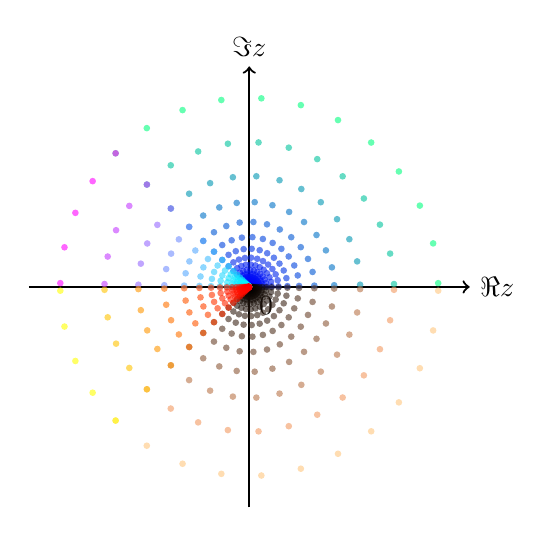
\begin{tikzpicture}[scale=0.8]

\draw[->, thick] (-3.5,0) -- (3.5,0) node[right] {$\Re z$};
\draw[->, thick] (0,-3.5) -- (0,3.5) node[above] {$\Im z$};

\fill (0,0) circle (2.5pt) node[below right] {$0$};

\fill[color={rgb,255:red,0; green,0; blue,255}, opacity=0.60] (0.0065,0.0001) circle (1.5pt);
\fill[color={rgb,255:red,0; green,0; blue,255}, opacity=0.60] (0.0085,0.0002) circle (1.5pt);
\fill[color={rgb,255:red,0; green,0; blue,255}, opacity=0.60] (0.0111,0.0002) circle (1.5pt);
\fill[color={rgb,255:red,0; green,0; blue,255}, opacity=0.60] (0.0145,0.0003) circle (1.5pt);
\fill[color={rgb,255:red,0; green,1; blue,254}, opacity=0.60] (0.0190,0.0004) circle (1.5pt);
\fill[color={rgb,255:red,0; green,1; blue,254}, opacity=0.60] (0.0247,0.0005) circle (1.5pt);
\fill[color={rgb,255:red,0; green,2; blue,254}, opacity=0.60] (0.0323,0.0006) circle (1.5pt);
\fill[color={rgb,255:red,0; green,3; blue,253}, opacity=0.60] (0.0422,0.0008) circle (1.5pt);
\fill[color={rgb,255:red,0; green,4; blue,253}, opacity=0.60] (0.0550,0.0011) circle (1.5pt);
\fill[color={rgb,255:red,0; green,5; blue,252}, opacity=0.60] (0.0719,0.0014) circle (1.5pt);
\fill[color={rgb,255:red,0; green,7; blue,251}, opacity=0.60] (0.0938,0.0019) circle (1.5pt);
\fill[color={rgb,255:red,0; green,10; blue,250}, opacity=0.60] (0.1225,0.0024) circle (1.5pt);
\fill[color={rgb,255:red,0; green,13; blue,248}, opacity=0.60] (0.1599,0.0032) circle (1.5pt);
\fill[color={rgb,255:red,0; green,17; blue,246}, opacity=0.60] (0.2087,0.0042) circle (1.5pt);
\fill[color={rgb,255:red,0; green,22; blue,244}, opacity=0.60] (0.2724,0.0054) circle (1.5pt);
\fill[color={rgb,255:red,0; green,29; blue,240}, opacity=0.60] (0.3556,0.0071) circle (1.5pt);
\fill[color={rgb,255:red,0; green,39; blue,235}, opacity=0.60] (0.4642,0.0093) circle (1.5pt);
\fill[color={rgb,255:red,0; green,51; blue,229}, opacity=0.60] (0.6060,0.0121) circle (1.5pt);
\fill[color={rgb,255:red,0; green,67; blue,221}, opacity=0.60] (0.7911,0.0158) circle (1.5pt);
\fill[color={rgb,255:red,0; green,87; blue,211}, opacity=0.60] (1.0328,0.0207) circle (1.5pt);
\fill[color={rgb,255:red,0; green,113; blue,198}, opacity=0.60] (1.3482,0.0270) circle (1.5pt);
\fill[color={rgb,255:red,0; green,150; blue,179}, opacity=0.60] (1.7600,0.0352) circle (1.5pt);
\fill[color={rgb,255:red,0; green,195; blue,157}, opacity=0.60] (2.2976,0.0460) circle (1.5pt);
\fill[color={rgb,255:red,0; green,255; blue,127}, opacity=0.60] (2.9994,0.0600) circle (1.5pt);
\fill[color={rgb,255:red,0; green,0; blue,255}, opacity=0.60] (0.0049,0.0012) circle (1.5pt);
\fill[color={rgb,255:red,0; green,0; blue,255}, opacity=0.60] (0.0064,0.0015) circle (1.5pt);
\fill[color={rgb,255:red,0; green,0; blue,255}, opacity=0.60] (0.0083,0.0020) circle (1.5pt);
\fill[color={rgb,255:red,0; green,0; blue,255}, opacity=0.60] (0.0108,0.0026) circle (1.5pt);
\fill[color={rgb,255:red,0; green,0; blue,255}, opacity=0.60] (0.0141,0.0033) circle (1.5pt);
\fill[color={rgb,255:red,0; green,1; blue,254}, opacity=0.60] (0.0184,0.0044) circle (1.5pt);
\fill[color={rgb,255:red,0; green,1; blue,254}, opacity=0.60] (0.0241,0.0057) circle (1.5pt);
\fill[color={rgb,255:red,0; green,2; blue,254}, opacity=0.60] (0.0314,0.0074) circle (1.5pt);
\fill[color={rgb,255:red,0; green,3; blue,253}, opacity=0.60] (0.0410,0.0097) circle (1.5pt);
\fill[color={rgb,255:red,0; green,4; blue,253}, opacity=0.60] (0.0536,0.0127) circle (1.5pt);
\fill[color={rgb,255:red,0; green,5; blue,252}, opacity=0.60] (0.0699,0.0166) circle (1.5pt);
\fill[color={rgb,255:red,0; green,7; blue,251}, opacity=0.60] (0.0913,0.0216) circle (1.5pt);
\fill[color={rgb,255:red,0; green,10; blue,250}, opacity=0.60] (0.1192,0.0282) circle (1.5pt);
\fill[color={rgb,255:red,0; green,13; blue,248}, opacity=0.60] (0.1556,0.0368) circle (1.5pt);
\fill[color={rgb,255:red,0; green,17; blue,246}, opacity=0.60] (0.2031,0.0481) circle (1.5pt);
\fill[color={rgb,255:red,0; green,22; blue,244}, opacity=0.60] (0.2651,0.0627) circle (1.5pt);
\fill[color={rgb,255:red,0; green,29; blue,240}, opacity=0.60] (0.3461,0.0819) circle (1.5pt);
\fill[color={rgb,255:red,0; green,39; blue,235}, opacity=0.60] (0.4518,0.1069) circle (1.5pt);
\fill[color={rgb,255:red,0; green,51; blue,229}, opacity=0.60] (0.5899,0.1396) circle (1.5pt);
\fill[color={rgb,255:red,0; green,67; blue,221}, opacity=0.60] (0.7700,0.1822) circle (1.5pt);
\fill[color={rgb,255:red,0; green,87; blue,211}, opacity=0.60] (1.0052,0.2379) circle (1.5pt);
\fill[color={rgb,255:red,0; green,113; blue,198}, opacity=0.60] (1.3123,0.3106) circle (1.5pt);
\fill[color={rgb,255:red,0; green,150; blue,179}, opacity=0.60] (1.7131,0.4054) circle (1.5pt);
\fill[color={rgb,255:red,0; green,195; blue,157}, opacity=0.60] (2.2363,0.5292) circle (1.5pt);
\fill[color={rgb,255:red,0; green,255; blue,127}, opacity=0.60] (2.9194,0.6909) circle (1.5pt);
\fill[color={rgb,255:red,0; green,0; blue,255}, opacity=0.60] (0.0045,0.0022) circle (1.5pt);
\fill[color={rgb,255:red,0; green,0; blue,255}, opacity=0.60] (0.0059,0.0028) circle (1.5pt);
\fill[color={rgb,255:red,0; green,0; blue,255}, opacity=0.60] (0.0077,0.0037) circle (1.5pt);
\fill[color={rgb,255:red,0; green,0; blue,255}, opacity=0.60] (0.0100,0.0048) circle (1.5pt);
\fill[color={rgb,255:red,0; green,0; blue,255}, opacity=0.60] (0.0131,0.0062) circle (1.5pt);
\fill[color={rgb,255:red,0; green,1; blue,254}, opacity=0.60] (0.0171,0.0082) circle (1.5pt);
\fill[color={rgb,255:red,0; green,1; blue,254}, opacity=0.60] (0.0223,0.0106) circle (1.5pt);
\fill[color={rgb,255:red,0; green,2; blue,254}, opacity=0.60] (0.0292,0.0139) circle (1.5pt);
\fill[color={rgb,255:red,0; green,3; blue,253}, opacity=0.60] (0.0381,0.0181) circle (1.5pt);
\fill[color={rgb,255:red,0; green,4; blue,253}, opacity=0.60] (0.0497,0.0237) circle (1.5pt);
\fill[color={rgb,255:red,0; green,5; blue,252}, opacity=0.60] (0.0649,0.0309) circle (1.5pt);
\fill[color={rgb,255:red,0; green,7; blue,251}, opacity=0.60] (0.0847,0.0404) circle (1.5pt);
\fill[color={rgb,255:red,0; green,10; blue,250}, opacity=0.60] (0.1106,0.0527) circle (1.5pt);
\fill[color={rgb,255:red,0; green,13; blue,248}, opacity=0.60] (0.1443,0.0688) circle (1.5pt);
\fill[color={rgb,255:red,0; green,17; blue,246}, opacity=0.60] (0.1884,0.0898) circle (1.5pt);
\fill[color={rgb,255:red,0; green,22; blue,244}, opacity=0.60] (0.2460,0.1172) circle (1.5pt);
\fill[color={rgb,255:red,0; green,29; blue,240}, opacity=0.60] (0.3211,0.1530) circle (1.5pt);
\fill[color={rgb,255:red,0; green,39; blue,235}, opacity=0.60] (0.4192,0.1998) circle (1.5pt);
\fill[color={rgb,255:red,0; green,51; blue,229}, opacity=0.60] (0.5472,0.2608) circle (1.5pt);
\fill[color={rgb,255:red,0; green,67; blue,221}, opacity=0.60] (0.7143,0.3405) circle (1.5pt);
\fill[color={rgb,255:red,0; green,87; blue,211}, opacity=0.60] (0.9325,0.4444) circle (1.5pt);
\fill[color={rgb,255:red,0; green,113; blue,198}, opacity=0.60] (1.2173,0.5802) circle (1.5pt);
\fill[color={rgb,255:red,0; green,150; blue,179}, opacity=0.60] (1.5891,0.7574) circle (1.5pt);
\fill[color={rgb,255:red,0; green,195; blue,157}, opacity=0.60] (2.0745,0.9887) circle (1.5pt);
\fill[color={rgb,255:red,0; green,255; blue,127}, opacity=0.60] (2.7081,1.2907) circle (1.5pt);
\fill[color={rgb,255:red,0; green,0; blue,255}, opacity=0.60] (0.0040,0.0031) circle (1.5pt);
\fill[color={rgb,255:red,0; green,0; blue,255}, opacity=0.60] (0.0052,0.0040) circle (1.5pt);
\fill[color={rgb,255:red,0; green,0; blue,255}, opacity=0.60] (0.0067,0.0052) circle (1.5pt);
\fill[color={rgb,255:red,0; green,0; blue,255}, opacity=0.60] (0.0088,0.0068) circle (1.5pt);
\fill[color={rgb,255:red,0; green,0; blue,255}, opacity=0.60] (0.0115,0.0089) circle (1.5pt);
\fill[color={rgb,255:red,0; green,1; blue,254}, opacity=0.60] (0.0150,0.0116) circle (1.5pt);
\fill[color={rgb,255:red,0; green,1; blue,254}, opacity=0.60] (0.0196,0.0151) circle (1.5pt);
\fill[color={rgb,255:red,0; green,2; blue,254}, opacity=0.60] (0.0256,0.0197) circle (1.5pt);
\fill[color={rgb,255:red,0; green,3; blue,253}, opacity=0.60] (0.0334,0.0258) circle (1.5pt);
\fill[color={rgb,255:red,0; green,4; blue,253}, opacity=0.60] (0.0436,0.0336) circle (1.5pt);
\fill[color={rgb,255:red,0; green,5; blue,252}, opacity=0.60] (0.0569,0.0439) circle (1.5pt);
\fill[color={rgb,255:red,0; green,7; blue,251}, opacity=0.60] (0.0743,0.0573) circle (1.5pt);
\fill[color={rgb,255:red,0; green,10; blue,250}, opacity=0.60] (0.0970,0.0748) circle (1.5pt);
\fill[color={rgb,255:red,0; green,13; blue,248}, opacity=0.60] (0.1266,0.0977) circle (1.5pt);
\fill[color={rgb,255:red,0; green,17; blue,246}, opacity=0.60] (0.1653,0.1275) circle (1.5pt);
\fill[color={rgb,255:red,0; green,22; blue,244}, opacity=0.60] (0.2157,0.1664) circle (1.5pt);
\fill[color={rgb,255:red,0; green,29; blue,240}, opacity=0.60] (0.2816,0.2173) circle (1.5pt);
\fill[color={rgb,255:red,0; green,39; blue,235}, opacity=0.60] (0.3676,0.2836) circle (1.5pt);
\fill[color={rgb,255:red,0; green,51; blue,229}, opacity=0.60] (0.4799,0.3703) circle (1.5pt);
\fill[color={rgb,255:red,0; green,67; blue,221}, opacity=0.60] (0.6265,0.4834) circle (1.5pt);
\fill[color={rgb,255:red,0; green,87; blue,211}, opacity=0.60] (0.8179,0.6310) circle (1.5pt);
\fill[color={rgb,255:red,0; green,113; blue,198}, opacity=0.60] (1.0677,0.8237) circle (1.5pt);
\fill[color={rgb,255:red,0; green,150; blue,179}, opacity=0.60] (1.3938,1.0753) circle (1.5pt);
\fill[color={rgb,255:red,0; green,195; blue,157}, opacity=0.60] (1.8195,1.4038) circle (1.5pt);
\fill[color={rgb,255:red,0; green,255; blue,127}, opacity=0.60] (2.3752,1.8326) circle (1.5pt);
\fill[color={rgb,255:red,0; green,0; blue,255}, opacity=0.60] (0.0032,0.0038) circle (1.5pt);
\fill[color={rgb,255:red,0; green,0; blue,255}, opacity=0.60] (0.0042,0.0050) circle (1.5pt);
\fill[color={rgb,255:red,0; green,0; blue,255}, opacity=0.60] (0.0055,0.0065) circle (1.5pt);
\fill[color={rgb,255:red,0; green,0; blue,255}, opacity=0.60] (0.0072,0.0085) circle (1.5pt);
\fill[color={rgb,255:red,0; green,0; blue,255}, opacity=0.60] (0.0094,0.0111) circle (1.5pt);
\fill[color={rgb,255:red,0; green,1; blue,254}, opacity=0.60] (0.0122,0.0145) circle (1.5pt);
\fill[color={rgb,255:red,0; green,1; blue,254}, opacity=0.60] (0.0160,0.0189) circle (1.5pt);
\fill[color={rgb,255:red,0; green,2; blue,254}, opacity=0.60] (0.0208,0.0247) circle (1.5pt);
\fill[color={rgb,255:red,0; green,3; blue,253}, opacity=0.60] (0.0272,0.0322) circle (1.5pt);
\fill[color={rgb,255:red,0; green,4; blue,253}, opacity=0.60] (0.0355,0.0421) circle (1.5pt);
\fill[color={rgb,255:red,0; green,5; blue,252}, opacity=0.60] (0.0464,0.0549) circle (1.5pt);
\fill[color={rgb,255:red,0; green,7; blue,251}, opacity=0.60] (0.0605,0.0717) circle (1.5pt);
\fill[color={rgb,255:red,0; green,10; blue,250}, opacity=0.60] (0.0790,0.0936) circle (1.5pt);
\fill[color={rgb,255:red,0; green,13; blue,248}, opacity=0.60] (0.1032,0.1222) circle (1.5pt);
\fill[color={rgb,255:red,0; green,17; blue,246}, opacity=0.60] (0.1347,0.1595) circle (1.5pt);
\fill[color={rgb,255:red,0; green,22; blue,244}, opacity=0.60] (0.1758,0.2082) circle (1.5pt);
\fill[color={rgb,255:red,0; green,29; blue,240}, opacity=0.60] (0.2295,0.2718) circle (1.5pt);
\fill[color={rgb,255:red,0; green,39; blue,235}, opacity=0.60] (0.2996,0.3548) circle (1.5pt);
\fill[color={rgb,255:red,0; green,51; blue,229}, opacity=0.60] (0.3911,0.4631) circle (1.5pt);
\fill[color={rgb,255:red,0; green,67; blue,221}, opacity=0.60] (0.5105,0.6046) circle (1.5pt);
\fill[color={rgb,255:red,0; green,87; blue,211}, opacity=0.60] (0.6665,0.7892) circle (1.5pt);
\fill[color={rgb,255:red,0; green,113; blue,198}, opacity=0.60] (0.8700,1.0303) circle (1.5pt);
\fill[color={rgb,255:red,0; green,150; blue,179}, opacity=0.60] (1.1358,1.3450) circle (1.5pt);
\fill[color={rgb,255:red,0; green,195; blue,157}, opacity=0.60] (1.4827,1.7558) circle (1.5pt);
\fill[color={rgb,255:red,0; green,255; blue,127}, opacity=0.60] (1.9356,2.2921) circle (1.5pt);
\fill[color={rgb,255:red,0; green,0; blue,255}, opacity=0.60] (0.0023,0.0044) circle (1.5pt);
\fill[color={rgb,255:red,0; green,0; blue,255}, opacity=0.60] (0.0031,0.0058) circle (1.5pt);
\fill[color={rgb,255:red,0; green,0; blue,255}, opacity=0.60] (0.0040,0.0075) circle (1.5pt);
\fill[color={rgb,255:red,0; green,0; blue,255}, opacity=0.60] (0.0052,0.0098) circle (1.5pt);
\fill[color={rgb,255:red,0; green,0; blue,255}, opacity=0.60] (0.0068,0.0128) circle (1.5pt);
\fill[color={rgb,255:red,0; green,1; blue,254}, opacity=0.60] (0.0089,0.0167) circle (1.5pt);
\fill[color={rgb,255:red,0; green,1; blue,254}, opacity=0.60] (0.0116,0.0218) circle (1.5pt);
\fill[color={rgb,255:red,0; green,2; blue,254}, opacity=0.60] (0.0152,0.0285) circle (1.5pt);
\fill[color={rgb,255:red,0; green,3; blue,253}, opacity=0.60] (0.0198,0.0372) circle (1.5pt);
\fill[color={rgb,255:red,0; green,4; blue,253}, opacity=0.60] (0.0259,0.0486) circle (1.5pt);
\fill[color={rgb,255:red,0; green,5; blue,252}, opacity=0.60] (0.0338,0.0634) circle (1.5pt);
\fill[color={rgb,255:red,0; green,7; blue,251}, opacity=0.60] (0.0441,0.0828) circle (1.5pt);
\fill[color={rgb,255:red,0; green,10; blue,250}, opacity=0.60] (0.0575,0.1081) circle (1.5pt);
\fill[color={rgb,255:red,0; green,13; blue,248}, opacity=0.60] (0.0751,0.1412) circle (1.5pt);
\fill[color={rgb,255:red,0; green,17; blue,246}, opacity=0.60] (0.0980,0.1843) circle (1.5pt);
\fill[color={rgb,255:red,0; green,22; blue,244}, opacity=0.60] (0.1280,0.2405) circle (1.5pt);
\fill[color={rgb,255:red,0; green,29; blue,240}, opacity=0.60] (0.1670,0.3140) circle (1.5pt);
\fill[color={rgb,255:red,0; green,39; blue,235}, opacity=0.60] (0.2181,0.4099) circle (1.5pt);
\fill[color={rgb,255:red,0; green,51; blue,229}, opacity=0.60] (0.2847,0.5351) circle (1.5pt);
\fill[color={rgb,255:red,0; green,67; blue,221}, opacity=0.60] (0.3716,0.6986) circle (1.5pt);
\fill[color={rgb,255:red,0; green,87; blue,211}, opacity=0.60] (0.4851,0.9120) circle (1.5pt);
\fill[color={rgb,255:red,0; green,113; blue,198}, opacity=0.60] (0.6333,1.1905) circle (1.5pt);
\fill[color={rgb,255:red,0; green,150; blue,179}, opacity=0.60] (0.8268,1.5542) circle (1.5pt);
\fill[color={rgb,255:red,0; green,195; blue,157}, opacity=0.60] (1.0793,2.0289) circle (1.5pt);
\fill[color={rgb,255:red,0; green,255; blue,127}, opacity=0.60] (1.4089,2.6486) circle (1.5pt);
\fill[color={rgb,255:red,0; green,0; blue,255}, opacity=0.60] (0.0014,0.0048) circle (1.5pt);
\fill[color={rgb,255:red,0; green,0; blue,255}, opacity=0.60] (0.0018,0.0063) circle (1.5pt);
\fill[color={rgb,255:red,0; green,0; blue,255}, opacity=0.60] (0.0023,0.0082) circle (1.5pt);
\fill[color={rgb,255:red,0; green,0; blue,255}, opacity=0.60] (0.0030,0.0107) circle (1.5pt);
\fill[color={rgb,255:red,0; green,0; blue,255}, opacity=0.60] (0.0040,0.0140) circle (1.5pt);
\fill[color={rgb,255:red,0; green,1; blue,254}, opacity=0.60] (0.0052,0.0182) circle (1.5pt);
\fill[color={rgb,255:red,0; green,1; blue,254}, opacity=0.60] (0.0068,0.0238) circle (1.5pt);
\fill[color={rgb,255:red,0; green,2; blue,254}, opacity=0.60] (0.0088,0.0311) circle (1.5pt);
\fill[color={rgb,255:red,0; green,3; blue,253}, opacity=0.60] (0.0115,0.0406) circle (1.5pt);
\fill[color={rgb,255:red,0; green,4; blue,253}, opacity=0.60] (0.0150,0.0530) circle (1.5pt);
\fill[color={rgb,255:red,0; green,5; blue,252}, opacity=0.60] (0.0196,0.0691) circle (1.5pt);
\fill[color={rgb,255:red,0; green,7; blue,251}, opacity=0.60] (0.0256,0.0903) circle (1.5pt);
\fill[color={rgb,255:red,0; green,10; blue,250}, opacity=0.60] (0.0334,0.1178) circle (1.5pt);
\fill[color={rgb,255:red,0; green,13; blue,248}, opacity=0.60] (0.0436,0.1538) circle (1.5pt);
\fill[color={rgb,255:red,0; green,17; blue,246}, opacity=0.60] (0.0570,0.2008) circle (1.5pt);
\fill[color={rgb,255:red,0; green,22; blue,244}, opacity=0.60] (0.0744,0.2621) circle (1.5pt);
\fill[color={rgb,255:red,0; green,29; blue,240}, opacity=0.60] (0.0971,0.3422) circle (1.5pt);
\fill[color={rgb,255:red,0; green,39; blue,235}, opacity=0.60] (0.1268,0.4467) circle (1.5pt);
\fill[color={rgb,255:red,0; green,51; blue,229}, opacity=0.60] (0.1655,0.5831) circle (1.5pt);
\fill[color={rgb,255:red,0; green,67; blue,221}, opacity=0.60] (0.2160,0.7612) circle (1.5pt);
\fill[color={rgb,255:red,0; green,87; blue,211}, opacity=0.60] (0.2820,0.9938) circle (1.5pt);
\fill[color={rgb,255:red,0; green,113; blue,198}, opacity=0.60] (0.3681,1.2973) circle (1.5pt);
\fill[color={rgb,255:red,0; green,150; blue,179}, opacity=0.60] (0.4806,1.6935) circle (1.5pt);
\fill[color={rgb,255:red,0; green,195; blue,157}, opacity=0.60] (0.6274,2.2108) circle (1.5pt);
\fill[color={rgb,255:red,0; green,255; blue,127}, opacity=0.60] (0.8190,2.8860) circle (1.5pt);
\fill[color={rgb,255:red,0; green,0; blue,255}, opacity=0.60] (0.0003,0.0050) circle (1.5pt);
\fill[color={rgb,255:red,0; green,0; blue,255}, opacity=0.60] (0.0004,0.0065) circle (1.5pt);
\fill[color={rgb,255:red,0; green,0; blue,255}, opacity=0.60] (0.0005,0.0085) circle (1.5pt);
\fill[color={rgb,255:red,0; green,0; blue,255}, opacity=0.60] (0.0007,0.0111) circle (1.5pt);
\fill[color={rgb,255:red,0; green,0; blue,255}, opacity=0.60] (0.0009,0.0145) circle (1.5pt);
\fill[color={rgb,255:red,0; green,1; blue,254}, opacity=0.60] (0.0012,0.0189) circle (1.5pt);
\fill[color={rgb,255:red,0; green,1; blue,254}, opacity=0.60] (0.0016,0.0247) circle (1.5pt);
\fill[color={rgb,255:red,0; green,2; blue,254}, opacity=0.60] (0.0021,0.0322) circle (1.5pt);
\fill[color={rgb,255:red,0; green,3; blue,253}, opacity=0.60] (0.0027,0.0421) circle (1.5pt);
\fill[color={rgb,255:red,0; green,4; blue,253}, opacity=0.60] (0.0035,0.0549) circle (1.5pt);
\fill[color={rgb,255:red,0; green,5; blue,252}, opacity=0.60] (0.0046,0.0717) circle (1.5pt);
\fill[color={rgb,255:red,0; green,7; blue,251}, opacity=0.60] (0.0060,0.0936) circle (1.5pt);
\fill[color={rgb,255:red,0; green,10; blue,250}, opacity=0.60] (0.0078,0.1222) circle (1.5pt);
\fill[color={rgb,255:red,0; green,13; blue,248}, opacity=0.60] (0.0102,0.1596) circle (1.5pt);
\fill[color={rgb,255:red,0; green,17; blue,246}, opacity=0.60] (0.0134,0.2083) circle (1.5pt);
\fill[color={rgb,255:red,0; green,22; blue,244}, opacity=0.60] (0.0175,0.2719) circle (1.5pt);
\fill[color={rgb,255:red,0; green,29; blue,240}, opacity=0.60] (0.0228,0.3550) circle (1.5pt);
\fill[color={rgb,255:red,0; green,39; blue,235}, opacity=0.60] (0.0298,0.4634) circle (1.5pt);
\fill[color={rgb,255:red,0; green,51; blue,229}, opacity=0.60] (0.0388,0.6049) circle (1.5pt);
\fill[color={rgb,255:red,0; green,67; blue,221}, opacity=0.60] (0.0507,0.7897) circle (1.5pt);
\fill[color={rgb,255:red,0; green,87; blue,211}, opacity=0.60] (0.0662,1.0309) circle (1.5pt);
\fill[color={rgb,255:red,0; green,113; blue,198}, opacity=0.60] (0.0864,1.3457) circle (1.5pt);
\fill[color={rgb,255:red,0; green,150; blue,179}, opacity=0.60] (0.1128,1.7568) circle (1.5pt);
\fill[color={rgb,255:red,0; green,195; blue,157}, opacity=0.60] (0.1473,2.2934) circle (1.5pt);
\fill[color={rgb,255:red,0; green,255; blue,127}, opacity=0.60] (0.1922,2.9938) circle (1.5pt);
\fill[color={rgb,255:red,0; green,0; blue,255}, opacity=0.60] (-0.0007,0.0049) circle (1.5pt);
\fill[color={rgb,255:red,0; green,0; blue,255}, opacity=0.60] (-0.0010,0.0065) circle (1.5pt);
\fill[color={rgb,255:red,0; green,0; blue,255}, opacity=0.60] (-0.0013,0.0084) circle (1.5pt);
\fill[color={rgb,255:red,0; green,0; blue,255}, opacity=0.60] (-0.0016,0.0110) circle (1.5pt);
\fill[color={rgb,255:red,0; green,0; blue,255}, opacity=0.60] (-0.0021,0.0144) circle (1.5pt);
\fill[color={rgb,255:red,0; green,1; blue,254}, opacity=0.60] (-0.0028,0.0187) circle (1.5pt);
\fill[color={rgb,255:red,0; green,1; blue,254}, opacity=0.60] (-0.0037,0.0245) circle (1.5pt);
\fill[color={rgb,255:red,0; green,2; blue,254}, opacity=0.60] (-0.0048,0.0319) circle (1.5pt);
\fill[color={rgb,255:red,0; green,3; blue,253}, opacity=0.60] (-0.0062,0.0417) circle (1.5pt);
\fill[color={rgb,255:red,0; green,4; blue,253}, opacity=0.60] (-0.0081,0.0544) circle (1.5pt);
\fill[color={rgb,255:red,0; green,5; blue,252}, opacity=0.60] (-0.0106,0.0711) circle (1.5pt);
\fill[color={rgb,255:red,0; green,7; blue,251}, opacity=0.60] (-0.0139,0.0928) circle (1.5pt);
\fill[color={rgb,255:red,0; green,10; blue,250}, opacity=0.60] (-0.0181,0.1211) circle (1.5pt);
\fill[color={rgb,255:red,0; green,13; blue,248}, opacity=0.60] (-0.0236,0.1581) circle (1.5pt);
\fill[color={rgb,255:red,0; green,17; blue,246}, opacity=0.60] (-0.0308,0.2064) circle (1.5pt);
\fill[color={rgb,255:red,0; green,22; blue,244}, opacity=0.60] (-0.0402,0.2695) circle (1.5pt);
\fill[color={rgb,255:red,0; green,29; blue,240}, opacity=0.60] (-0.0525,0.3518) circle (1.5pt);
\fill[color={rgb,255:red,0; green,39; blue,235}, opacity=0.60] (-0.0686,0.4592) circle (1.5pt);
\fill[color={rgb,255:red,0; green,51; blue,229}, opacity=0.60] (-0.0895,0.5995) circle (1.5pt);
\fill[color={rgb,255:red,0; green,67; blue,221}, opacity=0.60] (-0.1169,0.7826) circle (1.5pt);
\fill[color={rgb,255:red,0; green,87; blue,211}, opacity=0.60] (-0.1526,1.0217) circle (1.5pt);
\fill[color={rgb,255:red,0; green,113; blue,198}, opacity=0.60] (-0.1992,1.3337) circle (1.5pt);
\fill[color={rgb,255:red,0; green,150; blue,179}, opacity=0.60] (-0.2600,1.7411) circle (1.5pt);
\fill[color={rgb,255:red,0; green,195; blue,157}, opacity=0.60] (-0.3395,2.2729) circle (1.5pt);
\fill[color={rgb,255:red,0; green,255; blue,127}, opacity=0.60] (-0.4431,2.9671) circle (1.5pt);
\fill[color={rgb,255:red,0; green,0; blue,255}, opacity=0.60] (-0.0018,0.0047) circle (1.5pt);
\fill[color={rgb,255:red,0; green,0; blue,255}, opacity=0.60] (-0.0023,0.0061) circle (1.5pt);
\fill[color={rgb,255:red,0; green,0; blue,255}, opacity=0.60] (-0.0030,0.0080) circle (1.5pt);
\fill[color={rgb,255:red,0; green,0; blue,255}, opacity=0.60] (-0.0039,0.0104) circle (1.5pt);
\fill[color={rgb,255:red,0; green,0; blue,255}, opacity=0.60] (-0.0051,0.0136) circle (1.5pt);
\fill[color={rgb,255:red,0; green,1; blue,254}, opacity=0.60] (-0.0067,0.0177) circle (1.5pt);
\fill[color={rgb,255:red,0; green,1; blue,254}, opacity=0.60] (-0.0087,0.0232) circle (1.5pt);
\fill[color={rgb,255:red,0; green,2; blue,254}, opacity=0.60] (-0.0114,0.0302) circle (1.5pt);
\fill[color={rgb,255:red,0; green,3; blue,253}, opacity=0.60] (-0.0149,0.0395) circle (1.5pt);
\fill[color={rgb,255:red,0; green,4; blue,253}, opacity=0.60] (-0.0194,0.0515) circle (1.5pt);
\fill[color={rgb,255:red,0; green,5; blue,252}, opacity=0.60] (-0.0254,0.0672) circle (1.5pt);
\fill[color={rgb,255:red,0; green,7; blue,251}, opacity=0.60] (-0.0331,0.0878) circle (1.5pt);
\fill[color={rgb,255:red,0; green,10; blue,250}, opacity=0.60] (-0.0432,0.1146) circle (1.5pt);
\fill[color={rgb,255:red,0; green,13; blue,248}, opacity=0.60] (-0.0564,0.1496) circle (1.5pt);
\fill[color={rgb,255:red,0; green,17; blue,246}, opacity=0.60] (-0.0736,0.1953) circle (1.5pt);
\fill[color={rgb,255:red,0; green,22; blue,244}, opacity=0.60] (-0.0961,0.2549) circle (1.5pt);
\fill[color={rgb,255:red,0; green,29; blue,240}, opacity=0.60] (-0.1255,0.3328) circle (1.5pt);
\fill[color={rgb,255:red,0; green,39; blue,235}, opacity=0.60] (-0.1638,0.4345) circle (1.5pt);
\fill[color={rgb,255:red,0; green,51; blue,229}, opacity=0.60] (-0.2139,0.5672) circle (1.5pt);
\fill[color={rgb,255:red,0; green,67; blue,221}, opacity=0.60] (-0.2792,0.7404) circle (1.5pt);
\fill[color={rgb,255:red,0; green,87; blue,211}, opacity=0.60] (-0.3645,0.9665) circle (1.5pt);
\fill[color={rgb,255:red,0; green,113; blue,198}, opacity=0.60] (-0.4758,1.2618) circle (1.5pt);
\fill[color={rgb,255:red,0; green,150; blue,179}, opacity=0.60] (-0.6212,1.6471) circle (1.5pt);
\fill[color={rgb,255:red,0; green,195; blue,157}, opacity=0.60] (-0.8109,2.1503) circle (1.5pt);
\fill[color={rgb,255:red,0; green,255; blue,127}, opacity=0.60] (-1.0586,2.8070) circle (1.5pt);
\fill[color={rgb,255:red,0; green,0; blue,255}, opacity=0.60] (-0.0027,0.0042) circle (1.5pt);
\fill[color={rgb,255:red,0; green,0; blue,255}, opacity=0.60] (-0.0035,0.0055) circle (1.5pt);
\fill[color={rgb,255:red,0; green,0; blue,255}, opacity=0.60] (-0.0046,0.0072) circle (1.5pt);
\fill[color={rgb,255:red,0; green,0; blue,255}, opacity=0.60] (-0.0060,0.0093) circle (1.5pt);
\fill[color={rgb,255:red,0; green,0; blue,255}, opacity=0.60] (-0.0079,0.0122) circle (1.5pt);
\fill[color={rgb,255:red,0; green,1; blue,254}, opacity=0.60] (-0.0103,0.0159) circle (1.5pt);
\fill[color={rgb,255:red,0; green,1; blue,254}, opacity=0.60] (-0.0134,0.0208) circle (1.5pt);
\fill[color={rgb,255:red,0; green,2; blue,254}, opacity=0.60] (-0.0175,0.0271) circle (1.5pt);
\fill[color={rgb,255:red,0; green,3; blue,253}, opacity=0.60] (-0.0229,0.0354) circle (1.5pt);
\fill[color={rgb,255:red,0; green,4; blue,253}, opacity=0.60] (-0.0298,0.0463) circle (1.5pt);
\fill[color={rgb,255:red,0; green,5; blue,252}, opacity=0.60] (-0.0390,0.0604) circle (1.5pt);
\fill[color={rgb,255:red,0; green,7; blue,251}, opacity=0.60] (-0.0509,0.0788) circle (1.5pt);
\fill[color={rgb,255:red,0; green,10; blue,250}, opacity=0.60] (-0.0664,0.1029) circle (1.5pt);
\fill[color={rgb,255:red,0; green,13; blue,248}, opacity=0.60] (-0.0867,0.1343) circle (1.5pt);
\fill[color={rgb,255:red,0; green,17; blue,246}, opacity=0.60] (-0.1132,0.1754) circle (1.5pt);
\fill[color={rgb,255:red,0; green,22; blue,244}, opacity=0.60] (-0.1477,0.2289) circle (1.5pt);
\fill[color={rgb,255:red,0; green,29; blue,240}, opacity=0.60] (-0.1928,0.2989) circle (1.5pt);
\fill[color={rgb,255:red,0; green,39; blue,235}, opacity=0.60] (-0.2517,0.3902) circle (1.5pt);
\fill[color={rgb,255:red,0; green,51; blue,229}, opacity=0.60] (-0.3286,0.5093) circle (1.5pt);
\fill[color={rgb,255:red,0; green,67; blue,221}, opacity=0.60] (-0.4290,0.6649) circle (1.5pt);
\fill[color={rgb,255:red,0; green,87; blue,211}, opacity=0.60] (-0.5601,0.8680) circle (1.5pt);
\fill[color={rgb,255:red,0; green,113; blue,198}, opacity=0.60] (-0.7311,1.1331) circle (1.5pt);
\fill[color={rgb,255:red,0; green,150; blue,179}, opacity=0.60] (-0.9544,1.4792) circle (1.5pt);
\fill[color={rgb,255:red,0; green,195; blue,157}, opacity=0.60] (-1.2459,1.9310) circle (1.5pt);
\fill[color={rgb,255:red,0; green,255; blue,127}, opacity=0.60] (-1.6265,2.5208) circle (1.5pt);
\fill[color={rgb,255:red,0; green,0; blue,255}, opacity=0.60] (-0.0035,0.0035) circle (1.5pt);
\fill[color={rgb,255:red,0; green,0; blue,255}, opacity=0.60] (-0.0046,0.0046) circle (1.5pt);
\fill[color={rgb,255:red,0; green,0; blue,255}, opacity=0.60] (-0.0060,0.0060) circle (1.5pt);
\fill[color={rgb,255:red,0; green,0; blue,255}, opacity=0.60] (-0.0079,0.0079) circle (1.5pt);
\fill[color={rgb,255:red,0; green,0; blue,255}, opacity=0.60] (-0.0103,0.0103) circle (1.5pt);
\fill[color={rgb,255:red,0; green,1; blue,254}, opacity=0.60] (-0.0134,0.0134) circle (1.5pt);
\fill[color={rgb,255:red,0; green,1; blue,254}, opacity=0.60] (-0.0175,0.0175) circle (1.5pt);
\fill[color={rgb,255:red,0; green,2; blue,254}, opacity=0.60] (-0.0228,0.0228) circle (1.5pt);
\fill[color={rgb,255:red,0; green,3; blue,253}, opacity=0.60] (-0.0298,0.0298) circle (1.5pt);
\fill[color={rgb,255:red,0; green,4; blue,253}, opacity=0.60] (-0.0389,0.0389) circle (1.5pt);
\fill[color={rgb,255:red,0; green,5; blue,252}, opacity=0.60] (-0.0508,0.0508) circle (1.5pt);
\fill[color={rgb,255:red,0; green,7; blue,251}, opacity=0.60] (-0.0663,0.0663) circle (1.5pt);
\fill[color={rgb,255:red,0; green,10; blue,250}, opacity=0.60] (-0.0866,0.0866) circle (1.5pt);
\fill[color={rgb,255:red,0; green,13; blue,248}, opacity=0.60] (-0.1131,0.1131) circle (1.5pt);
\fill[color={rgb,255:red,0; green,17; blue,246}, opacity=0.60] (-0.1476,0.1476) circle (1.5pt);
\fill[color={rgb,255:red,0; green,22; blue,244}, opacity=0.60] (-0.1927,0.1927) circle (1.5pt);
\fill[color={rgb,255:red,0; green,29; blue,240}, opacity=0.60] (-0.2515,0.2515) circle (1.5pt);
\fill[color={rgb,255:red,0; green,39; blue,235}, opacity=0.60] (-0.3283,0.3283) circle (1.5pt);
\fill[color={rgb,255:red,0; green,51; blue,229}, opacity=0.60] (-0.4286,0.4286) circle (1.5pt);
\fill[color={rgb,255:red,0; green,67; blue,221}, opacity=0.60] (-0.5595,0.5595) circle (1.5pt);
\fill[color={rgb,255:red,0; green,87; blue,211}, opacity=0.60] (-0.7304,0.7304) circle (1.5pt);
\fill[color={rgb,255:red,0; green,113; blue,198}, opacity=0.60] (-0.9535,0.9535) circle (1.5pt);
\fill[color={rgb,255:red,0; green,150; blue,179}, opacity=0.60] (-1.2448,1.2448) circle (1.5pt);
\fill[color={rgb,255:red,0; green,195; blue,157}, opacity=0.60] (-1.6250,1.6250) circle (1.5pt);
\fill[color={rgb,255:red,0; green,255; blue,127}, opacity=0.60] (-2.1213,2.1213) circle (1.5pt);
\fill[color={rgb,255:red,0; green,0; blue,0}, opacity=0.60] (-0.0035,-0.0035) circle (1.5pt);
\fill[color={rgb,255:red,0; green,0; blue,0}, opacity=0.60] (-0.0046,-0.0046) circle (1.5pt);
\fill[color={rgb,255:red,0; green,0; blue,0}, opacity=0.60] (-0.0060,-0.0060) circle (1.5pt);
\fill[color={rgb,255:red,0; green,0; blue,0}, opacity=0.60] (-0.0079,-0.0079) circle (1.5pt);
\fill[color={rgb,255:red,0; green,0; blue,0}, opacity=0.60] (-0.0103,-0.0103) circle (1.5pt);
\fill[color={rgb,255:red,1; green,0; blue,0}, opacity=0.60] (-0.0134,-0.0134) circle (1.5pt);
\fill[color={rgb,255:red,1; green,0; blue,0}, opacity=0.60] (-0.0175,-0.0175) circle (1.5pt);
\fill[color={rgb,255:red,2; green,1; blue,0}, opacity=0.60] (-0.0228,-0.0228) circle (1.5pt);
\fill[color={rgb,255:red,3; green,2; blue,1}, opacity=0.60] (-0.0298,-0.0298) circle (1.5pt);
\fill[color={rgb,255:red,4; green,3; blue,1}, opacity=0.60] (-0.0389,-0.0389) circle (1.5pt);
\fill[color={rgb,255:red,6; green,3; blue,2}, opacity=0.60] (-0.0508,-0.0508) circle (1.5pt);
\fill[color={rgb,255:red,8; green,5; blue,3}, opacity=0.60] (-0.0663,-0.0663) circle (1.5pt);
\fill[color={rgb,255:red,12; green,7; blue,4}, opacity=0.60] (-0.0866,-0.0866) circle (1.5pt);
\fill[color={rgb,255:red,16; green,10; blue,6}, opacity=0.60] (-0.1131,-0.1131) circle (1.5pt);
\fill[color={rgb,255:red,20; green,13; blue,8}, opacity=0.60] (-0.1476,-0.1476) circle (1.5pt);
\fill[color={rgb,255:red,27; green,17; blue,10}, opacity=0.60] (-0.1927,-0.1927) circle (1.5pt);
\fill[color={rgb,255:red,35; green,22; blue,14}, opacity=0.60] (-0.2515,-0.2515) circle (1.5pt);
\fill[color={rgb,255:red,48; green,30; blue,19}, opacity=0.60] (-0.3283,-0.3283) circle (1.5pt);
\fill[color={rgb,255:red,62; green,39; blue,25}, opacity=0.60] (-0.4286,-0.4286) circle (1.5pt);
\fill[color={rgb,255:red,82; green,52; blue,33}, opacity=0.60] (-0.5595,-0.5595) circle (1.5pt);
\fill[color={rgb,255:red,107; green,67; blue,43}, opacity=0.60] (-0.7304,-0.7304) circle (1.5pt);
\fill[color={rgb,255:red,140; green,89; blue,56}, opacity=0.60] (-0.9535,-0.9535) circle (1.5pt);
\fill[color={rgb,255:red,185; green,117; blue,74}, opacity=0.60] (-1.2448,-1.2448) circle (1.5pt);
\fill[color={rgb,255:red,242; green,153; blue,97}, opacity=0.60] (-1.6250,-1.6250) circle (1.5pt);
\fill[color={rgb,255:red,255; green,199; blue,126}, opacity=0.60] (-2.1213,-2.1213) circle (1.5pt);
\fill[color={rgb,255:red,0; green,0; blue,0}, opacity=0.60] (-0.0027,-0.0042) circle (1.5pt);
\fill[color={rgb,255:red,0; green,0; blue,0}, opacity=0.60] (-0.0035,-0.0055) circle (1.5pt);
\fill[color={rgb,255:red,0; green,0; blue,0}, opacity=0.60] (-0.0046,-0.0072) circle (1.5pt);
\fill[color={rgb,255:red,0; green,0; blue,0}, opacity=0.60] (-0.0060,-0.0093) circle (1.5pt);
\fill[color={rgb,255:red,0; green,0; blue,0}, opacity=0.60] (-0.0079,-0.0122) circle (1.5pt);
\fill[color={rgb,255:red,1; green,0; blue,0}, opacity=0.60] (-0.0103,-0.0159) circle (1.5pt);
\fill[color={rgb,255:red,1; green,0; blue,0}, opacity=0.60] (-0.0134,-0.0208) circle (1.5pt);
\fill[color={rgb,255:red,2; green,1; blue,0}, opacity=0.60] (-0.0175,-0.0271) circle (1.5pt);
\fill[color={rgb,255:red,3; green,2; blue,1}, opacity=0.60] (-0.0229,-0.0354) circle (1.5pt);
\fill[color={rgb,255:red,4; green,3; blue,1}, opacity=0.60] (-0.0298,-0.0463) circle (1.5pt);
\fill[color={rgb,255:red,6; green,3; blue,2}, opacity=0.60] (-0.0390,-0.0604) circle (1.5pt);
\fill[color={rgb,255:red,8; green,5; blue,3}, opacity=0.60] (-0.0509,-0.0788) circle (1.5pt);
\fill[color={rgb,255:red,12; green,7; blue,4}, opacity=0.60] (-0.0664,-0.1029) circle (1.5pt);
\fill[color={rgb,255:red,16; green,10; blue,6}, opacity=0.60] (-0.0867,-0.1343) circle (1.5pt);
\fill[color={rgb,255:red,20; green,13; blue,8}, opacity=0.60] (-0.1132,-0.1754) circle (1.5pt);
\fill[color={rgb,255:red,27; green,17; blue,10}, opacity=0.60] (-0.1477,-0.2289) circle (1.5pt);
\fill[color={rgb,255:red,35; green,22; blue,14}, opacity=0.60] (-0.1928,-0.2989) circle (1.5pt);
\fill[color={rgb,255:red,48; green,30; blue,19}, opacity=0.60] (-0.2517,-0.3902) circle (1.5pt);
\fill[color={rgb,255:red,62; green,39; blue,25}, opacity=0.60] (-0.3286,-0.5093) circle (1.5pt);
\fill[color={rgb,255:red,82; green,52; blue,33}, opacity=0.60] (-0.4290,-0.6649) circle (1.5pt);
\fill[color={rgb,255:red,107; green,67; blue,43}, opacity=0.60] (-0.5601,-0.8680) circle (1.5pt);
\fill[color={rgb,255:red,140; green,89; blue,56}, opacity=0.60] (-0.7311,-1.1331) circle (1.5pt);
\fill[color={rgb,255:red,185; green,117; blue,74}, opacity=0.60] (-0.9544,-1.4792) circle (1.5pt);
\fill[color={rgb,255:red,242; green,153; blue,97}, opacity=0.60] (-1.2459,-1.9310) circle (1.5pt);
\fill[color={rgb,255:red,255; green,199; blue,126}, opacity=0.60] (-1.6265,-2.5208) circle (1.5pt);
\fill[color={rgb,255:red,0; green,0; blue,0}, opacity=0.60] (-0.0018,-0.0047) circle (1.5pt);
\fill[color={rgb,255:red,0; green,0; blue,0}, opacity=0.60] (-0.0023,-0.0061) circle (1.5pt);
\fill[color={rgb,255:red,0; green,0; blue,0}, opacity=0.60] (-0.0030,-0.0080) circle (1.5pt);
\fill[color={rgb,255:red,0; green,0; blue,0}, opacity=0.60] (-0.0039,-0.0104) circle (1.5pt);
\fill[color={rgb,255:red,0; green,0; blue,0}, opacity=0.60] (-0.0051,-0.0136) circle (1.5pt);
\fill[color={rgb,255:red,1; green,0; blue,0}, opacity=0.60] (-0.0067,-0.0177) circle (1.5pt);
\fill[color={rgb,255:red,1; green,0; blue,0}, opacity=0.60] (-0.0087,-0.0232) circle (1.5pt);
\fill[color={rgb,255:red,2; green,1; blue,0}, opacity=0.60] (-0.0114,-0.0302) circle (1.5pt);
\fill[color={rgb,255:red,3; green,2; blue,1}, opacity=0.60] (-0.0149,-0.0395) circle (1.5pt);
\fill[color={rgb,255:red,4; green,3; blue,1}, opacity=0.60] (-0.0194,-0.0515) circle (1.5pt);
\fill[color={rgb,255:red,6; green,3; blue,2}, opacity=0.60] (-0.0254,-0.0672) circle (1.5pt);
\fill[color={rgb,255:red,8; green,5; blue,3}, opacity=0.60] (-0.0331,-0.0878) circle (1.5pt);
\fill[color={rgb,255:red,12; green,7; blue,4}, opacity=0.60] (-0.0432,-0.1146) circle (1.5pt);
\fill[color={rgb,255:red,16; green,10; blue,6}, opacity=0.60] (-0.0564,-0.1496) circle (1.5pt);
\fill[color={rgb,255:red,20; green,13; blue,8}, opacity=0.60] (-0.0736,-0.1953) circle (1.5pt);
\fill[color={rgb,255:red,27; green,17; blue,10}, opacity=0.60] (-0.0961,-0.2549) circle (1.5pt);
\fill[color={rgb,255:red,35; green,22; blue,14}, opacity=0.60] (-0.1255,-0.3328) circle (1.5pt);
\fill[color={rgb,255:red,48; green,30; blue,19}, opacity=0.60] (-0.1638,-0.4345) circle (1.5pt);
\fill[color={rgb,255:red,62; green,39; blue,25}, opacity=0.60] (-0.2139,-0.5672) circle (1.5pt);
\fill[color={rgb,255:red,82; green,52; blue,33}, opacity=0.60] (-0.2792,-0.7404) circle (1.5pt);
\fill[color={rgb,255:red,107; green,67; blue,43}, opacity=0.60] (-0.3645,-0.9665) circle (1.5pt);
\fill[color={rgb,255:red,140; green,89; blue,56}, opacity=0.60] (-0.4758,-1.2618) circle (1.5pt);
\fill[color={rgb,255:red,185; green,117; blue,74}, opacity=0.60] (-0.6212,-1.6471) circle (1.5pt);
\fill[color={rgb,255:red,242; green,153; blue,97}, opacity=0.60] (-0.8109,-2.1503) circle (1.5pt);
\fill[color={rgb,255:red,255; green,199; blue,126}, opacity=0.60] (-1.0586,-2.8070) circle (1.5pt);
\fill[color={rgb,255:red,0; green,0; blue,0}, opacity=0.60] (-0.0007,-0.0049) circle (1.5pt);
\fill[color={rgb,255:red,0; green,0; blue,0}, opacity=0.60] (-0.0010,-0.0065) circle (1.5pt);
\fill[color={rgb,255:red,0; green,0; blue,0}, opacity=0.60] (-0.0013,-0.0084) circle (1.5pt);
\fill[color={rgb,255:red,0; green,0; blue,0}, opacity=0.60] (-0.0016,-0.0110) circle (1.5pt);
\fill[color={rgb,255:red,0; green,0; blue,0}, opacity=0.60] (-0.0021,-0.0144) circle (1.5pt);
\fill[color={rgb,255:red,1; green,0; blue,0}, opacity=0.60] (-0.0028,-0.0187) circle (1.5pt);
\fill[color={rgb,255:red,1; green,0; blue,0}, opacity=0.60] (-0.0037,-0.0245) circle (1.5pt);
\fill[color={rgb,255:red,2; green,1; blue,0}, opacity=0.60] (-0.0048,-0.0319) circle (1.5pt);
\fill[color={rgb,255:red,3; green,2; blue,1}, opacity=0.60] (-0.0062,-0.0417) circle (1.5pt);
\fill[color={rgb,255:red,4; green,3; blue,1}, opacity=0.60] (-0.0081,-0.0544) circle (1.5pt);
\fill[color={rgb,255:red,6; green,3; blue,2}, opacity=0.60] (-0.0106,-0.0711) circle (1.5pt);
\fill[color={rgb,255:red,8; green,5; blue,3}, opacity=0.60] (-0.0139,-0.0928) circle (1.5pt);
\fill[color={rgb,255:red,12; green,7; blue,4}, opacity=0.60] (-0.0181,-0.1211) circle (1.5pt);
\fill[color={rgb,255:red,16; green,10; blue,6}, opacity=0.60] (-0.0236,-0.1581) circle (1.5pt);
\fill[color={rgb,255:red,20; green,13; blue,8}, opacity=0.60] (-0.0308,-0.2064) circle (1.5pt);
\fill[color={rgb,255:red,27; green,17; blue,10}, opacity=0.60] (-0.0402,-0.2695) circle (1.5pt);
\fill[color={rgb,255:red,35; green,22; blue,14}, opacity=0.60] (-0.0525,-0.3518) circle (1.5pt);
\fill[color={rgb,255:red,48; green,30; blue,19}, opacity=0.60] (-0.0686,-0.4592) circle (1.5pt);
\fill[color={rgb,255:red,62; green,39; blue,25}, opacity=0.60] (-0.0895,-0.5995) circle (1.5pt);
\fill[color={rgb,255:red,82; green,52; blue,33}, opacity=0.60] (-0.1169,-0.7826) circle (1.5pt);
\fill[color={rgb,255:red,107; green,67; blue,43}, opacity=0.60] (-0.1526,-1.0217) circle (1.5pt);
\fill[color={rgb,255:red,140; green,89; blue,56}, opacity=0.60] (-0.1992,-1.3337) circle (1.5pt);
\fill[color={rgb,255:red,185; green,117; blue,74}, opacity=0.60] (-0.2600,-1.7411) circle (1.5pt);
\fill[color={rgb,255:red,242; green,153; blue,97}, opacity=0.60] (-0.3395,-2.2729) circle (1.5pt);
\fill[color={rgb,255:red,255; green,199; blue,126}, opacity=0.60] (-0.4431,-2.9671) circle (1.5pt);
\fill[color={rgb,255:red,0; green,0; blue,0}, opacity=0.60] (0.0003,-0.0050) circle (1.5pt);
\fill[color={rgb,255:red,0; green,0; blue,0}, opacity=0.60] (0.0004,-0.0065) circle (1.5pt);
\fill[color={rgb,255:red,0; green,0; blue,0}, opacity=0.60] (0.0005,-0.0085) circle (1.5pt);
\fill[color={rgb,255:red,0; green,0; blue,0}, opacity=0.60] (0.0007,-0.0111) circle (1.5pt);
\fill[color={rgb,255:red,0; green,0; blue,0}, opacity=0.60] (0.0009,-0.0145) circle (1.5pt);
\fill[color={rgb,255:red,1; green,0; blue,0}, opacity=0.60] (0.0012,-0.0189) circle (1.5pt);
\fill[color={rgb,255:red,1; green,0; blue,0}, opacity=0.60] (0.0016,-0.0247) circle (1.5pt);
\fill[color={rgb,255:red,2; green,1; blue,0}, opacity=0.60] (0.0021,-0.0322) circle (1.5pt);
\fill[color={rgb,255:red,3; green,2; blue,1}, opacity=0.60] (0.0027,-0.0421) circle (1.5pt);
\fill[color={rgb,255:red,4; green,3; blue,1}, opacity=0.60] (0.0035,-0.0549) circle (1.5pt);
\fill[color={rgb,255:red,6; green,3; blue,2}, opacity=0.60] (0.0046,-0.0717) circle (1.5pt);
\fill[color={rgb,255:red,8; green,5; blue,3}, opacity=0.60] (0.0060,-0.0936) circle (1.5pt);
\fill[color={rgb,255:red,12; green,7; blue,4}, opacity=0.60] (0.0078,-0.1222) circle (1.5pt);
\fill[color={rgb,255:red,16; green,10; blue,6}, opacity=0.60] (0.0102,-0.1596) circle (1.5pt);
\fill[color={rgb,255:red,20; green,13; blue,8}, opacity=0.60] (0.0134,-0.2083) circle (1.5pt);
\fill[color={rgb,255:red,27; green,17; blue,10}, opacity=0.60] (0.0175,-0.2719) circle (1.5pt);
\fill[color={rgb,255:red,35; green,22; blue,14}, opacity=0.60] (0.0228,-0.3550) circle (1.5pt);
\fill[color={rgb,255:red,48; green,30; blue,19}, opacity=0.60] (0.0298,-0.4634) circle (1.5pt);
\fill[color={rgb,255:red,62; green,39; blue,25}, opacity=0.60] (0.0388,-0.6049) circle (1.5pt);
\fill[color={rgb,255:red,82; green,52; blue,33}, opacity=0.60] (0.0507,-0.7897) circle (1.5pt);
\fill[color={rgb,255:red,107; green,67; blue,43}, opacity=0.60] (0.0662,-1.0309) circle (1.5pt);
\fill[color={rgb,255:red,140; green,89; blue,56}, opacity=0.60] (0.0864,-1.3457) circle (1.5pt);
\fill[color={rgb,255:red,185; green,117; blue,74}, opacity=0.60] (0.1128,-1.7568) circle (1.5pt);
\fill[color={rgb,255:red,242; green,153; blue,97}, opacity=0.60] (0.1473,-2.2934) circle (1.5pt);
\fill[color={rgb,255:red,255; green,199; blue,126}, opacity=0.60] (0.1922,-2.9938) circle (1.5pt);
\fill[color={rgb,255:red,0; green,0; blue,0}, opacity=0.60] (0.0014,-0.0048) circle (1.5pt);
\fill[color={rgb,255:red,0; green,0; blue,0}, opacity=0.60] (0.0018,-0.0063) circle (1.5pt);
\fill[color={rgb,255:red,0; green,0; blue,0}, opacity=0.60] (0.0023,-0.0082) circle (1.5pt);
\fill[color={rgb,255:red,0; green,0; blue,0}, opacity=0.60] (0.0030,-0.0107) circle (1.5pt);
\fill[color={rgb,255:red,0; green,0; blue,0}, opacity=0.60] (0.0040,-0.0140) circle (1.5pt);
\fill[color={rgb,255:red,1; green,0; blue,0}, opacity=0.60] (0.0052,-0.0182) circle (1.5pt);
\fill[color={rgb,255:red,1; green,0; blue,0}, opacity=0.60] (0.0068,-0.0238) circle (1.5pt);
\fill[color={rgb,255:red,2; green,1; blue,0}, opacity=0.60] (0.0088,-0.0311) circle (1.5pt);
\fill[color={rgb,255:red,3; green,2; blue,1}, opacity=0.60] (0.0115,-0.0406) circle (1.5pt);
\fill[color={rgb,255:red,4; green,3; blue,1}, opacity=0.60] (0.0150,-0.0530) circle (1.5pt);
\fill[color={rgb,255:red,6; green,3; blue,2}, opacity=0.60] (0.0196,-0.0691) circle (1.5pt);
\fill[color={rgb,255:red,8; green,5; blue,3}, opacity=0.60] (0.0256,-0.0903) circle (1.5pt);
\fill[color={rgb,255:red,12; green,7; blue,4}, opacity=0.60] (0.0334,-0.1178) circle (1.5pt);
\fill[color={rgb,255:red,16; green,10; blue,6}, opacity=0.60] (0.0436,-0.1538) circle (1.5pt);
\fill[color={rgb,255:red,20; green,13; blue,8}, opacity=0.60] (0.0570,-0.2008) circle (1.5pt);
\fill[color={rgb,255:red,27; green,17; blue,10}, opacity=0.60] (0.0744,-0.2621) circle (1.5pt);
\fill[color={rgb,255:red,35; green,22; blue,14}, opacity=0.60] (0.0971,-0.3422) circle (1.5pt);
\fill[color={rgb,255:red,48; green,30; blue,19}, opacity=0.60] (0.1268,-0.4467) circle (1.5pt);
\fill[color={rgb,255:red,62; green,39; blue,25}, opacity=0.60] (0.1655,-0.5831) circle (1.5pt);
\fill[color={rgb,255:red,82; green,52; blue,33}, opacity=0.60] (0.2160,-0.7612) circle (1.5pt);
\fill[color={rgb,255:red,107; green,67; blue,43}, opacity=0.60] (0.2820,-0.9938) circle (1.5pt);
\fill[color={rgb,255:red,140; green,89; blue,56}, opacity=0.60] (0.3681,-1.2973) circle (1.5pt);
\fill[color={rgb,255:red,185; green,117; blue,74}, opacity=0.60] (0.4806,-1.6935) circle (1.5pt);
\fill[color={rgb,255:red,242; green,153; blue,97}, opacity=0.60] (0.6274,-2.2108) circle (1.5pt);
\fill[color={rgb,255:red,255; green,199; blue,126}, opacity=0.60] (0.8190,-2.8860) circle (1.5pt);
\fill[color={rgb,255:red,0; green,0; blue,0}, opacity=0.60] (0.0023,-0.0044) circle (1.5pt);
\fill[color={rgb,255:red,0; green,0; blue,0}, opacity=0.60] (0.0031,-0.0058) circle (1.5pt);
\fill[color={rgb,255:red,0; green,0; blue,0}, opacity=0.60] (0.0040,-0.0075) circle (1.5pt);
\fill[color={rgb,255:red,0; green,0; blue,0}, opacity=0.60] (0.0052,-0.0098) circle (1.5pt);
\fill[color={rgb,255:red,0; green,0; blue,0}, opacity=0.60] (0.0068,-0.0128) circle (1.5pt);
\fill[color={rgb,255:red,1; green,0; blue,0}, opacity=0.60] (0.0089,-0.0167) circle (1.5pt);
\fill[color={rgb,255:red,1; green,0; blue,0}, opacity=0.60] (0.0116,-0.0218) circle (1.5pt);
\fill[color={rgb,255:red,2; green,1; blue,0}, opacity=0.60] (0.0152,-0.0285) circle (1.5pt);
\fill[color={rgb,255:red,3; green,2; blue,1}, opacity=0.60] (0.0198,-0.0372) circle (1.5pt);
\fill[color={rgb,255:red,4; green,3; blue,1}, opacity=0.60] (0.0259,-0.0486) circle (1.5pt);
\fill[color={rgb,255:red,6; green,3; blue,2}, opacity=0.60] (0.0338,-0.0634) circle (1.5pt);
\fill[color={rgb,255:red,8; green,5; blue,3}, opacity=0.60] (0.0441,-0.0828) circle (1.5pt);
\fill[color={rgb,255:red,12; green,7; blue,4}, opacity=0.60] (0.0575,-0.1081) circle (1.5pt);
\fill[color={rgb,255:red,16; green,10; blue,6}, opacity=0.60] (0.0751,-0.1412) circle (1.5pt);
\fill[color={rgb,255:red,20; green,13; blue,8}, opacity=0.60] (0.0980,-0.1843) circle (1.5pt);
\fill[color={rgb,255:red,27; green,17; blue,10}, opacity=0.60] (0.1280,-0.2405) circle (1.5pt);
\fill[color={rgb,255:red,35; green,22; blue,14}, opacity=0.60] (0.1670,-0.3140) circle (1.5pt);
\fill[color={rgb,255:red,48; green,30; blue,19}, opacity=0.60] (0.2181,-0.4099) circle (1.5pt);
\fill[color={rgb,255:red,62; green,39; blue,25}, opacity=0.60] (0.2847,-0.5351) circle (1.5pt);
\fill[color={rgb,255:red,82; green,52; blue,33}, opacity=0.60] (0.3716,-0.6986) circle (1.5pt);
\fill[color={rgb,255:red,107; green,67; blue,43}, opacity=0.60] (0.4851,-0.9120) circle (1.5pt);
\fill[color={rgb,255:red,140; green,89; blue,56}, opacity=0.60] (0.6333,-1.1905) circle (1.5pt);
\fill[color={rgb,255:red,185; green,117; blue,74}, opacity=0.60] (0.8268,-1.5542) circle (1.5pt);
\fill[color={rgb,255:red,242; green,153; blue,97}, opacity=0.60] (1.0793,-2.0289) circle (1.5pt);
\fill[color={rgb,255:red,255; green,199; blue,126}, opacity=0.60] (1.4089,-2.6486) circle (1.5pt);
\fill[color={rgb,255:red,0; green,0; blue,0}, opacity=0.60] (0.0032,-0.0038) circle (1.5pt);
\fill[color={rgb,255:red,0; green,0; blue,0}, opacity=0.60] (0.0042,-0.0050) circle (1.5pt);
\fill[color={rgb,255:red,0; green,0; blue,0}, opacity=0.60] (0.0055,-0.0065) circle (1.5pt);
\fill[color={rgb,255:red,0; green,0; blue,0}, opacity=0.60] (0.0072,-0.0085) circle (1.5pt);
\fill[color={rgb,255:red,0; green,0; blue,0}, opacity=0.60] (0.0094,-0.0111) circle (1.5pt);
\fill[color={rgb,255:red,1; green,0; blue,0}, opacity=0.60] (0.0122,-0.0145) circle (1.5pt);
\fill[color={rgb,255:red,1; green,0; blue,0}, opacity=0.60] (0.0160,-0.0189) circle (1.5pt);
\fill[color={rgb,255:red,2; green,1; blue,0}, opacity=0.60] (0.0208,-0.0247) circle (1.5pt);
\fill[color={rgb,255:red,3; green,2; blue,1}, opacity=0.60] (0.0272,-0.0322) circle (1.5pt);
\fill[color={rgb,255:red,4; green,3; blue,1}, opacity=0.60] (0.0355,-0.0421) circle (1.5pt);
\fill[color={rgb,255:red,6; green,3; blue,2}, opacity=0.60] (0.0464,-0.0549) circle (1.5pt);
\fill[color={rgb,255:red,8; green,5; blue,3}, opacity=0.60] (0.0605,-0.0717) circle (1.5pt);
\fill[color={rgb,255:red,12; green,7; blue,4}, opacity=0.60] (0.0790,-0.0936) circle (1.5pt);
\fill[color={rgb,255:red,16; green,10; blue,6}, opacity=0.60] (0.1032,-0.1222) circle (1.5pt);
\fill[color={rgb,255:red,20; green,13; blue,8}, opacity=0.60] (0.1347,-0.1595) circle (1.5pt);
\fill[color={rgb,255:red,27; green,17; blue,10}, opacity=0.60] (0.1758,-0.2082) circle (1.5pt);
\fill[color={rgb,255:red,35; green,22; blue,14}, opacity=0.60] (0.2295,-0.2718) circle (1.5pt);
\fill[color={rgb,255:red,48; green,30; blue,19}, opacity=0.60] (0.2996,-0.3548) circle (1.5pt);
\fill[color={rgb,255:red,62; green,39; blue,25}, opacity=0.60] (0.3911,-0.4631) circle (1.5pt);
\fill[color={rgb,255:red,82; green,52; blue,33}, opacity=0.60] (0.5105,-0.6046) circle (1.5pt);
\fill[color={rgb,255:red,107; green,67; blue,43}, opacity=0.60] (0.6665,-0.7892) circle (1.5pt);
\fill[color={rgb,255:red,140; green,89; blue,56}, opacity=0.60] (0.8700,-1.0303) circle (1.5pt);
\fill[color={rgb,255:red,185; green,117; blue,74}, opacity=0.60] (1.1358,-1.3450) circle (1.5pt);
\fill[color={rgb,255:red,242; green,153; blue,97}, opacity=0.60] (1.4827,-1.7558) circle (1.5pt);
\fill[color={rgb,255:red,255; green,199; blue,126}, opacity=0.60] (1.9356,-2.2921) circle (1.5pt);
\fill[color={rgb,255:red,0; green,0; blue,0}, opacity=0.60] (0.0040,-0.0031) circle (1.5pt);
\fill[color={rgb,255:red,0; green,0; blue,0}, opacity=0.60] (0.0052,-0.0040) circle (1.5pt);
\fill[color={rgb,255:red,0; green,0; blue,0}, opacity=0.60] (0.0067,-0.0052) circle (1.5pt);
\fill[color={rgb,255:red,0; green,0; blue,0}, opacity=0.60] (0.0088,-0.0068) circle (1.5pt);
\fill[color={rgb,255:red,0; green,0; blue,0}, opacity=0.60] (0.0115,-0.0089) circle (1.5pt);
\fill[color={rgb,255:red,1; green,0; blue,0}, opacity=0.60] (0.0150,-0.0116) circle (1.5pt);
\fill[color={rgb,255:red,1; green,0; blue,0}, opacity=0.60] (0.0196,-0.0151) circle (1.5pt);
\fill[color={rgb,255:red,2; green,1; blue,0}, opacity=0.60] (0.0256,-0.0197) circle (1.5pt);
\fill[color={rgb,255:red,3; green,2; blue,1}, opacity=0.60] (0.0334,-0.0258) circle (1.5pt);
\fill[color={rgb,255:red,4; green,3; blue,1}, opacity=0.60] (0.0436,-0.0336) circle (1.5pt);
\fill[color={rgb,255:red,6; green,3; blue,2}, opacity=0.60] (0.0569,-0.0439) circle (1.5pt);
\fill[color={rgb,255:red,8; green,5; blue,3}, opacity=0.60] (0.0743,-0.0573) circle (1.5pt);
\fill[color={rgb,255:red,12; green,7; blue,4}, opacity=0.60] (0.0970,-0.0748) circle (1.5pt);
\fill[color={rgb,255:red,16; green,10; blue,6}, opacity=0.60] (0.1266,-0.0977) circle (1.5pt);
\fill[color={rgb,255:red,20; green,13; blue,8}, opacity=0.60] (0.1653,-0.1275) circle (1.5pt);
\fill[color={rgb,255:red,27; green,17; blue,10}, opacity=0.60] (0.2157,-0.1664) circle (1.5pt);
\fill[color={rgb,255:red,35; green,22; blue,14}, opacity=0.60] (0.2816,-0.2173) circle (1.5pt);
\fill[color={rgb,255:red,48; green,30; blue,19}, opacity=0.60] (0.3676,-0.2836) circle (1.5pt);
\fill[color={rgb,255:red,62; green,39; blue,25}, opacity=0.60] (0.4799,-0.3703) circle (1.5pt);
\fill[color={rgb,255:red,82; green,52; blue,33}, opacity=0.60] (0.6265,-0.4834) circle (1.5pt);
\fill[color={rgb,255:red,107; green,67; blue,43}, opacity=0.60] (0.8179,-0.6310) circle (1.5pt);
\fill[color={rgb,255:red,140; green,89; blue,56}, opacity=0.60] (1.0677,-0.8237) circle (1.5pt);
\fill[color={rgb,255:red,185; green,117; blue,74}, opacity=0.60] (1.3938,-1.0753) circle (1.5pt);
\fill[color={rgb,255:red,242; green,153; blue,97}, opacity=0.60] (1.8195,-1.4038) circle (1.5pt);
\fill[color={rgb,255:red,255; green,199; blue,126}, opacity=0.60] (2.3752,-1.8326) circle (1.5pt);
\fill[color={rgb,255:red,0; green,0; blue,0}, opacity=0.60] (0.0045,-0.0022) circle (1.5pt);
\fill[color={rgb,255:red,0; green,0; blue,0}, opacity=0.60] (0.0059,-0.0028) circle (1.5pt);
\fill[color={rgb,255:red,0; green,0; blue,0}, opacity=0.60] (0.0077,-0.0037) circle (1.5pt);
\fill[color={rgb,255:red,0; green,0; blue,0}, opacity=0.60] (0.0100,-0.0048) circle (1.5pt);
\fill[color={rgb,255:red,0; green,0; blue,0}, opacity=0.60] (0.0131,-0.0062) circle (1.5pt);
\fill[color={rgb,255:red,1; green,0; blue,0}, opacity=0.60] (0.0171,-0.0082) circle (1.5pt);
\fill[color={rgb,255:red,1; green,0; blue,0}, opacity=0.60] (0.0223,-0.0106) circle (1.5pt);
\fill[color={rgb,255:red,2; green,1; blue,0}, opacity=0.60] (0.0292,-0.0139) circle (1.5pt);
\fill[color={rgb,255:red,3; green,2; blue,1}, opacity=0.60] (0.0381,-0.0181) circle (1.5pt);
\fill[color={rgb,255:red,4; green,3; blue,1}, opacity=0.60] (0.0497,-0.0237) circle (1.5pt);
\fill[color={rgb,255:red,6; green,3; blue,2}, opacity=0.60] (0.0649,-0.0309) circle (1.5pt);
\fill[color={rgb,255:red,8; green,5; blue,3}, opacity=0.60] (0.0847,-0.0404) circle (1.5pt);
\fill[color={rgb,255:red,12; green,7; blue,4}, opacity=0.60] (0.1106,-0.0527) circle (1.5pt);
\fill[color={rgb,255:red,16; green,10; blue,6}, opacity=0.60] (0.1443,-0.0688) circle (1.5pt);
\fill[color={rgb,255:red,20; green,13; blue,8}, opacity=0.60] (0.1884,-0.0898) circle (1.5pt);
\fill[color={rgb,255:red,27; green,17; blue,10}, opacity=0.60] (0.2460,-0.1172) circle (1.5pt);
\fill[color={rgb,255:red,35; green,22; blue,14}, opacity=0.60] (0.3211,-0.1530) circle (1.5pt);
\fill[color={rgb,255:red,48; green,30; blue,19}, opacity=0.60] (0.4192,-0.1998) circle (1.5pt);
\fill[color={rgb,255:red,62; green,39; blue,25}, opacity=0.60] (0.5472,-0.2608) circle (1.5pt);
\fill[color={rgb,255:red,82; green,52; blue,33}, opacity=0.60] (0.7143,-0.3405) circle (1.5pt);
\fill[color={rgb,255:red,107; green,67; blue,43}, opacity=0.60] (0.9325,-0.4444) circle (1.5pt);
\fill[color={rgb,255:red,140; green,89; blue,56}, opacity=0.60] (1.2173,-0.5802) circle (1.5pt);
\fill[color={rgb,255:red,185; green,117; blue,74}, opacity=0.60] (1.5891,-0.7574) circle (1.5pt);
\fill[color={rgb,255:red,242; green,153; blue,97}, opacity=0.60] (2.0745,-0.9887) circle (1.5pt);
\fill[color={rgb,255:red,255; green,199; blue,126}, opacity=0.60] (2.7081,-1.2907) circle (1.5pt);
\fill[color={rgb,255:red,0; green,0; blue,0}, opacity=0.60] (0.0049,-0.0012) circle (1.5pt);
\fill[color={rgb,255:red,0; green,0; blue,0}, opacity=0.60] (0.0064,-0.0015) circle (1.5pt);
\fill[color={rgb,255:red,0; green,0; blue,0}, opacity=0.60] (0.0083,-0.0020) circle (1.5pt);
\fill[color={rgb,255:red,0; green,0; blue,0}, opacity=0.60] (0.0108,-0.0026) circle (1.5pt);
\fill[color={rgb,255:red,0; green,0; blue,0}, opacity=0.60] (0.0141,-0.0033) circle (1.5pt);
\fill[color={rgb,255:red,1; green,0; blue,0}, opacity=0.60] (0.0184,-0.0044) circle (1.5pt);
\fill[color={rgb,255:red,1; green,0; blue,0}, opacity=0.60] (0.0241,-0.0057) circle (1.5pt);
\fill[color={rgb,255:red,2; green,1; blue,0}, opacity=0.60] (0.0314,-0.0074) circle (1.5pt);
\fill[color={rgb,255:red,3; green,2; blue,1}, opacity=0.60] (0.0410,-0.0097) circle (1.5pt);
\fill[color={rgb,255:red,4; green,3; blue,1}, opacity=0.60] (0.0536,-0.0127) circle (1.5pt);
\fill[color={rgb,255:red,6; green,3; blue,2}, opacity=0.60] (0.0699,-0.0166) circle (1.5pt);
\fill[color={rgb,255:red,8; green,5; blue,3}, opacity=0.60] (0.0913,-0.0216) circle (1.5pt);
\fill[color={rgb,255:red,12; green,7; blue,4}, opacity=0.60] (0.1192,-0.0282) circle (1.5pt);
\fill[color={rgb,255:red,16; green,10; blue,6}, opacity=0.60] (0.1556,-0.0368) circle (1.5pt);
\fill[color={rgb,255:red,20; green,13; blue,8}, opacity=0.60] (0.2031,-0.0481) circle (1.5pt);
\fill[color={rgb,255:red,27; green,17; blue,10}, opacity=0.60] (0.2651,-0.0627) circle (1.5pt);
\fill[color={rgb,255:red,35; green,22; blue,14}, opacity=0.60] (0.3461,-0.0819) circle (1.5pt);
\fill[color={rgb,255:red,48; green,30; blue,19}, opacity=0.60] (0.4518,-0.1069) circle (1.5pt);
\fill[color={rgb,255:red,62; green,39; blue,25}, opacity=0.60] (0.5899,-0.1396) circle (1.5pt);
\fill[color={rgb,255:red,82; green,52; blue,33}, opacity=0.60] (0.7700,-0.1822) circle (1.5pt);
\fill[color={rgb,255:red,107; green,67; blue,43}, opacity=0.60] (1.0052,-0.2379) circle (1.5pt);
\fill[color={rgb,255:red,140; green,89; blue,56}, opacity=0.60] (1.3123,-0.3106) circle (1.5pt);
\fill[color={rgb,255:red,185; green,117; blue,74}, opacity=0.60] (1.7131,-0.4054) circle (1.5pt);
\fill[color={rgb,255:red,242; green,153; blue,97}, opacity=0.60] (2.2363,-0.5292) circle (1.5pt);
\fill[color={rgb,255:red,255; green,199; blue,126}, opacity=0.60] (2.9194,-0.6909) circle (1.5pt);
\fill[color={rgb,255:red,0; green,0; blue,0}, opacity=0.60] (0.0050,-0.0001) circle (1.5pt);
\fill[color={rgb,255:red,0; green,0; blue,0}, opacity=0.60] (0.0065,-0.0001) circle (1.5pt);
\fill[color={rgb,255:red,0; green,0; blue,0}, opacity=0.60] (0.0085,-0.0002) circle (1.5pt);
\fill[color={rgb,255:red,0; green,0; blue,0}, opacity=0.60] (0.0111,-0.0002) circle (1.5pt);
\fill[color={rgb,255:red,0; green,0; blue,0}, opacity=0.60] (0.0145,-0.0003) circle (1.5pt);
\fill[color={rgb,255:red,1; green,0; blue,0}, opacity=0.60] (0.0190,-0.0004) circle (1.5pt);
\fill[color={rgb,255:red,1; green,0; blue,0}, opacity=0.60] (0.0247,-0.0005) circle (1.5pt);
\fill[color={rgb,255:red,2; green,1; blue,0}, opacity=0.60] (0.0323,-0.0006) circle (1.5pt);
\fill[color={rgb,255:red,3; green,2; blue,1}, opacity=0.60] (0.0422,-0.0008) circle (1.5pt);
\fill[color={rgb,255:red,4; green,3; blue,1}, opacity=0.60] (0.0550,-0.0011) circle (1.5pt);
\fill[color={rgb,255:red,6; green,3; blue,2}, opacity=0.60] (0.0719,-0.0014) circle (1.5pt);
\fill[color={rgb,255:red,8; green,5; blue,3}, opacity=0.60] (0.0938,-0.0019) circle (1.5pt);
\fill[color={rgb,255:red,12; green,7; blue,4}, opacity=0.60] (0.1225,-0.0024) circle (1.5pt);
\fill[color={rgb,255:red,16; green,10; blue,6}, opacity=0.60] (0.1599,-0.0032) circle (1.5pt);
\fill[color={rgb,255:red,20; green,13; blue,8}, opacity=0.60] (0.2087,-0.0042) circle (1.5pt);
\fill[color={rgb,255:red,27; green,17; blue,10}, opacity=0.60] (0.2724,-0.0054) circle (1.5pt);
\fill[color={rgb,255:red,35; green,22; blue,14}, opacity=0.60] (0.3556,-0.0071) circle (1.5pt);
\fill[color={rgb,255:red,48; green,30; blue,19}, opacity=0.60] (0.4642,-0.0093) circle (1.5pt);
\fill[color={rgb,255:red,62; green,39; blue,25}, opacity=0.60] (0.6060,-0.0121) circle (1.5pt);
\fill[color={rgb,255:red,82; green,52; blue,33}, opacity=0.60] (0.7911,-0.0158) circle (1.5pt);
\fill[color={rgb,255:red,107; green,67; blue,43}, opacity=0.60] (1.0328,-0.0207) circle (1.5pt);
\fill[color={rgb,255:red,140; green,89; blue,56}, opacity=0.60] (1.3482,-0.0270) circle (1.5pt);
\fill[color={rgb,255:red,185; green,117; blue,74}, opacity=0.60] (1.7600,-0.0352) circle (1.5pt);
\fill[color={rgb,255:red,242; green,153; blue,97}, opacity=0.60] (2.2976,-0.0460) circle (1.5pt);
\fill[color={rgb,255:red,255; green,199; blue,126}, opacity=0.60] (2.9994,-0.0600) circle (1.5pt);
\fill[color={rgb,255:red,0; green,255; blue,255}, opacity=0.60] (-0.0035,0.0035) circle (1.5pt);
\fill[color={rgb,255:red,0; green,255; blue,255}, opacity=0.60] (-0.0046,0.0046) circle (1.5pt);
\fill[color={rgb,255:red,0; green,255; blue,255}, opacity=0.60] (-0.0060,0.0060) circle (1.5pt);
\fill[color={rgb,255:red,0; green,255; blue,255}, opacity=0.60] (-0.0079,0.0079) circle (1.5pt);
\fill[color={rgb,255:red,0; green,255; blue,255}, opacity=0.60] (-0.0103,0.0103) circle (1.5pt);
\fill[color={rgb,255:red,1; green,254; blue,255}, opacity=0.60] (-0.0134,0.0134) circle (1.5pt);
\fill[color={rgb,255:red,1; green,254; blue,255}, opacity=0.60] (-0.0175,0.0175) circle (1.5pt);
\fill[color={rgb,255:red,2; green,253; blue,255}, opacity=0.60] (-0.0228,0.0228) circle (1.5pt);
\fill[color={rgb,255:red,3; green,252; blue,255}, opacity=0.60] (-0.0298,0.0298) circle (1.5pt);
\fill[color={rgb,255:red,4; green,251; blue,255}, opacity=0.60] (-0.0389,0.0389) circle (1.5pt);
\fill[color={rgb,255:red,5; green,250; blue,255}, opacity=0.60] (-0.0508,0.0508) circle (1.5pt);
\fill[color={rgb,255:red,7; green,248; blue,255}, opacity=0.60] (-0.0663,0.0663) circle (1.5pt);
\fill[color={rgb,255:red,10; green,245; blue,255}, opacity=0.60] (-0.0866,0.0866) circle (1.5pt);
\fill[color={rgb,255:red,13; green,242; blue,255}, opacity=0.60] (-0.1131,0.1131) circle (1.5pt);
\fill[color={rgb,255:red,17; green,238; blue,255}, opacity=0.60] (-0.1476,0.1476) circle (1.5pt);
\fill[color={rgb,255:red,22; green,233; blue,255}, opacity=0.60] (-0.1927,0.1927) circle (1.5pt);
\fill[color={rgb,255:red,29; green,226; blue,255}, opacity=0.60] (-0.2515,0.2515) circle (1.5pt);
\fill[color={rgb,255:red,39; green,216; blue,255}, opacity=0.60] (-0.3283,0.3283) circle (1.5pt);
\fill[color={rgb,255:red,51; green,204; blue,255}, opacity=0.60] (-0.4286,0.4286) circle (1.5pt);
\fill[color={rgb,255:red,67; green,188; blue,255}, opacity=0.60] (-0.5595,0.5595) circle (1.5pt);
\fill[color={rgb,255:red,87; green,168; blue,255}, opacity=0.60] (-0.7304,0.7304) circle (1.5pt);
\fill[color={rgb,255:red,113; green,141; blue,255}, opacity=0.60] (-0.9535,0.9535) circle (1.5pt);
\fill[color={rgb,255:red,150; green,105; blue,255}, opacity=0.60] (-1.2448,1.2448) circle (1.5pt);
\fill[color={rgb,255:red,195; green,59; blue,255}, opacity=0.60] (-1.6250,1.6250) circle (1.5pt);
\fill[color={rgb,255:red,255; green,0; blue,255}, opacity=0.60] (-2.1213,2.1213) circle (1.5pt);
\fill[color={rgb,255:red,0; green,255; blue,255}, opacity=0.60] (-0.0041,0.0028) circle (1.5pt);
\fill[color={rgb,255:red,0; green,255; blue,255}, opacity=0.60] (-0.0054,0.0037) circle (1.5pt);
\fill[color={rgb,255:red,0; green,255; blue,255}, opacity=0.60] (-0.0071,0.0048) circle (1.5pt);
\fill[color={rgb,255:red,0; green,255; blue,255}, opacity=0.60] (-0.0092,0.0062) circle (1.5pt);
\fill[color={rgb,255:red,0; green,255; blue,255}, opacity=0.60] (-0.0120,0.0081) circle (1.5pt);
\fill[color={rgb,255:red,1; green,254; blue,255}, opacity=0.60] (-0.0157,0.0106) circle (1.5pt);
\fill[color={rgb,255:red,1; green,254; blue,255}, opacity=0.60] (-0.0205,0.0139) circle (1.5pt);
\fill[color={rgb,255:red,2; green,253; blue,255}, opacity=0.60] (-0.0268,0.0181) circle (1.5pt);
\fill[color={rgb,255:red,3; green,252; blue,255}, opacity=0.60] (-0.0349,0.0236) circle (1.5pt);
\fill[color={rgb,255:red,4; green,251; blue,255}, opacity=0.60] (-0.0456,0.0308) circle (1.5pt);
\fill[color={rgb,255:red,5; green,250; blue,255}, opacity=0.60] (-0.0596,0.0402) circle (1.5pt);
\fill[color={rgb,255:red,7; green,248; blue,255}, opacity=0.60] (-0.0777,0.0525) circle (1.5pt);
\fill[color={rgb,255:red,10; green,245; blue,255}, opacity=0.60] (-0.1015,0.0686) circle (1.5pt);
\fill[color={rgb,255:red,13; green,242; blue,255}, opacity=0.60] (-0.1325,0.0895) circle (1.5pt);
\fill[color={rgb,255:red,17; green,238; blue,255}, opacity=0.60] (-0.1730,0.1168) circle (1.5pt);
\fill[color={rgb,255:red,22; green,233; blue,255}, opacity=0.60] (-0.2258,0.1525) circle (1.5pt);
\fill[color={rgb,255:red,29; green,226; blue,255}, opacity=0.60] (-0.2948,0.1991) circle (1.5pt);
\fill[color={rgb,255:red,39; green,216; blue,255}, opacity=0.60] (-0.3848,0.2599) circle (1.5pt);
\fill[color={rgb,255:red,51; green,204; blue,255}, opacity=0.60] (-0.5023,0.3393) circle (1.5pt);
\fill[color={rgb,255:red,67; green,188; blue,255}, opacity=0.60] (-0.6557,0.4429) circle (1.5pt);
\fill[color={rgb,255:red,87; green,168; blue,255}, opacity=0.60] (-0.8560,0.5782) circle (1.5pt);
\fill[color={rgb,255:red,113; green,141; blue,255}, opacity=0.60] (-1.1175,0.7548) circle (1.5pt);
\fill[color={rgb,255:red,150; green,105; blue,255}, opacity=0.60] (-1.4588,0.9853) circle (1.5pt);
\fill[color={rgb,255:red,195; green,59; blue,255}, opacity=0.60] (-1.9044,1.2863) circle (1.5pt);
\fill[color={rgb,255:red,255; green,0; blue,255}, opacity=0.60] (-2.4860,1.6792) circle (1.5pt);
\fill[color={rgb,255:red,0; green,255; blue,255}, opacity=0.60] (-0.0046,0.0020) circle (1.5pt);
\fill[color={rgb,255:red,0; green,255; blue,255}, opacity=0.60] (-0.0060,0.0026) circle (1.5pt);
\fill[color={rgb,255:red,0; green,255; blue,255}, opacity=0.60] (-0.0078,0.0033) circle (1.5pt);
\fill[color={rgb,255:red,0; green,255; blue,255}, opacity=0.60] (-0.0102,0.0044) circle (1.5pt);
\fill[color={rgb,255:red,0; green,255; blue,255}, opacity=0.60] (-0.0134,0.0057) circle (1.5pt);
\fill[color={rgb,255:red,1; green,254; blue,255}, opacity=0.60] (-0.0174,0.0074) circle (1.5pt);
\fill[color={rgb,255:red,1; green,254; blue,255}, opacity=0.60] (-0.0228,0.0097) circle (1.5pt);
\fill[color={rgb,255:red,2; green,253; blue,255}, opacity=0.60] (-0.0297,0.0127) circle (1.5pt);
\fill[color={rgb,255:red,3; green,252; blue,255}, opacity=0.60] (-0.0388,0.0165) circle (1.5pt);
\fill[color={rgb,255:red,4; green,251; blue,255}, opacity=0.60] (-0.0506,0.0216) circle (1.5pt);
\fill[color={rgb,255:red,5; green,250; blue,255}, opacity=0.60] (-0.0661,0.0282) circle (1.5pt);
\fill[color={rgb,255:red,7; green,248; blue,255}, opacity=0.60] (-0.0863,0.0368) circle (1.5pt);
\fill[color={rgb,255:red,10; green,245; blue,255}, opacity=0.60] (-0.1127,0.0480) circle (1.5pt);
\fill[color={rgb,255:red,13; green,242; blue,255}, opacity=0.60] (-0.1471,0.0627) circle (1.5pt);
\fill[color={rgb,255:red,17; green,238; blue,255}, opacity=0.60] (-0.1920,0.0818) circle (1.5pt);
\fill[color={rgb,255:red,22; green,233; blue,255}, opacity=0.60] (-0.2507,0.1068) circle (1.5pt);
\fill[color={rgb,255:red,29; green,226; blue,255}, opacity=0.60] (-0.3272,0.1394) circle (1.5pt);
\fill[color={rgb,255:red,39; green,216; blue,255}, opacity=0.60] (-0.4272,0.1820) circle (1.5pt);
\fill[color={rgb,255:red,51; green,204; blue,255}, opacity=0.60] (-0.5577,0.2376) circle (1.5pt);
\fill[color={rgb,255:red,67; green,188; blue,255}, opacity=0.60] (-0.7280,0.3101) circle (1.5pt);
\fill[color={rgb,255:red,87; green,168; blue,255}, opacity=0.60] (-0.9504,0.4048) circle (1.5pt);
\fill[color={rgb,255:red,113; green,141; blue,255}, opacity=0.60] (-1.2406,0.5285) circle (1.5pt);
\fill[color={rgb,255:red,150; green,105; blue,255}, opacity=0.60] (-1.6196,0.6899) circle (1.5pt);
\fill[color={rgb,255:red,195; green,59; blue,255}, opacity=0.60] (-2.1142,0.9006) circle (1.5pt);
\fill[color={rgb,255:red,255; green,0; blue,255}, opacity=0.60] (-2.7600,1.1757) circle (1.5pt);
\fill[color={rgb,255:red,0; green,255; blue,255}, opacity=0.60] (-0.0049,0.0010) circle (1.5pt);
\fill[color={rgb,255:red,0; green,255; blue,255}, opacity=0.60] (-0.0064,0.0014) circle (1.5pt);
\fill[color={rgb,255:red,0; green,255; blue,255}, opacity=0.60] (-0.0083,0.0018) circle (1.5pt);
\fill[color={rgb,255:red,0; green,255; blue,255}, opacity=0.60] (-0.0109,0.0023) circle (1.5pt);
\fill[color={rgb,255:red,0; green,255; blue,255}, opacity=0.60] (-0.0142,0.0030) circle (1.5pt);
\fill[color={rgb,255:red,1; green,254; blue,255}, opacity=0.60] (-0.0185,0.0040) circle (1.5pt);
\fill[color={rgb,255:red,1; green,254; blue,255}, opacity=0.60] (-0.0242,0.0052) circle (1.5pt);
\fill[color={rgb,255:red,2; green,253; blue,255}, opacity=0.60] (-0.0316,0.0068) circle (1.5pt);
\fill[color={rgb,255:red,3; green,252; blue,255}, opacity=0.60] (-0.0412,0.0088) circle (1.5pt);
\fill[color={rgb,255:red,4; green,251; blue,255}, opacity=0.60] (-0.0538,0.0115) circle (1.5pt);
\fill[color={rgb,255:red,5; green,250; blue,255}, opacity=0.60] (-0.0703,0.0151) circle (1.5pt);
\fill[color={rgb,255:red,7; green,248; blue,255}, opacity=0.60] (-0.0917,0.0197) circle (1.5pt);
\fill[color={rgb,255:red,10; green,245; blue,255}, opacity=0.60] (-0.1197,0.0257) circle (1.5pt);
\fill[color={rgb,255:red,13; green,242; blue,255}, opacity=0.60] (-0.1563,0.0335) circle (1.5pt);
\fill[color={rgb,255:red,17; green,238; blue,255}, opacity=0.60] (-0.2041,0.0438) circle (1.5pt);
\fill[color={rgb,255:red,22; green,233; blue,255}, opacity=0.60] (-0.2664,0.0572) circle (1.5pt);
\fill[color={rgb,255:red,29; green,226; blue,255}, opacity=0.60] (-0.3478,0.0746) circle (1.5pt);
\fill[color={rgb,255:red,39; green,216; blue,255}, opacity=0.60] (-0.4540,0.0974) circle (1.5pt);
\fill[color={rgb,255:red,51; green,204; blue,255}, opacity=0.60] (-0.5927,0.1272) circle (1.5pt);
\fill[color={rgb,255:red,67; green,188; blue,255}, opacity=0.60] (-0.7737,0.1660) circle (1.5pt);
\fill[color={rgb,255:red,87; green,168; blue,255}, opacity=0.60] (-1.0100,0.2167) circle (1.5pt);
\fill[color={rgb,255:red,113; green,141; blue,255}, opacity=0.60] (-1.3185,0.2829) circle (1.5pt);
\fill[color={rgb,255:red,150; green,105; blue,255}, opacity=0.60] (-1.7212,0.3693) circle (1.5pt);
\fill[color={rgb,255:red,195; green,59; blue,255}, opacity=0.60] (-2.2469,0.4821) circle (1.5pt);
\fill[color={rgb,255:red,255; green,0; blue,255}, opacity=0.60] (-2.9332,0.6293) circle (1.5pt);
\fill[color={rgb,255:red,0; green,255; blue,255}, opacity=0.60] (-0.0050,0.0001) circle (1.5pt);
\fill[color={rgb,255:red,0; green,255; blue,255}, opacity=0.60] (-0.0065,0.0001) circle (1.5pt);
\fill[color={rgb,255:red,0; green,255; blue,255}, opacity=0.60] (-0.0085,0.0002) circle (1.5pt);
\fill[color={rgb,255:red,0; green,255; blue,255}, opacity=0.60] (-0.0111,0.0002) circle (1.5pt);
\fill[color={rgb,255:red,0; green,255; blue,255}, opacity=0.60] (-0.0145,0.0003) circle (1.5pt);
\fill[color={rgb,255:red,1; green,254; blue,255}, opacity=0.60] (-0.0190,0.0004) circle (1.5pt);
\fill[color={rgb,255:red,1; green,254; blue,255}, opacity=0.60] (-0.0247,0.0005) circle (1.5pt);
\fill[color={rgb,255:red,2; green,253; blue,255}, opacity=0.60] (-0.0323,0.0006) circle (1.5pt);
\fill[color={rgb,255:red,3; green,252; blue,255}, opacity=0.60] (-0.0422,0.0008) circle (1.5pt);
\fill[color={rgb,255:red,4; green,251; blue,255}, opacity=0.60] (-0.0550,0.0011) circle (1.5pt);
\fill[color={rgb,255:red,5; green,250; blue,255}, opacity=0.60] (-0.0719,0.0014) circle (1.5pt);
\fill[color={rgb,255:red,7; green,248; blue,255}, opacity=0.60] (-0.0938,0.0019) circle (1.5pt);
\fill[color={rgb,255:red,10; green,245; blue,255}, opacity=0.60] (-0.1225,0.0024) circle (1.5pt);
\fill[color={rgb,255:red,13; green,242; blue,255}, opacity=0.60] (-0.1599,0.0032) circle (1.5pt);
\fill[color={rgb,255:red,17; green,238; blue,255}, opacity=0.60] (-0.2087,0.0042) circle (1.5pt);
\fill[color={rgb,255:red,22; green,233; blue,255}, opacity=0.60] (-0.2724,0.0054) circle (1.5pt);
\fill[color={rgb,255:red,29; green,226; blue,255}, opacity=0.60] (-0.3556,0.0071) circle (1.5pt);
\fill[color={rgb,255:red,39; green,216; blue,255}, opacity=0.60] (-0.4642,0.0093) circle (1.5pt);
\fill[color={rgb,255:red,51; green,204; blue,255}, opacity=0.60] (-0.6060,0.0121) circle (1.5pt);
\fill[color={rgb,255:red,67; green,188; blue,255}, opacity=0.60] (-0.7911,0.0158) circle (1.5pt);
\fill[color={rgb,255:red,87; green,168; blue,255}, opacity=0.60] (-1.0328,0.0207) circle (1.5pt);
\fill[color={rgb,255:red,113; green,141; blue,255}, opacity=0.60] (-1.3482,0.0270) circle (1.5pt);
\fill[color={rgb,255:red,150; green,105; blue,255}, opacity=0.60] (-1.7600,0.0352) circle (1.5pt);
\fill[color={rgb,255:red,195; green,59; blue,255}, opacity=0.60] (-2.2976,0.0460) circle (1.5pt);
\fill[color={rgb,255:red,255; green,0; blue,255}, opacity=0.60] (-2.9994,0.0600) circle (1.5pt);
\fill[color={rgb,255:red,255; green,0; blue,0}, opacity=0.60] (-0.0050,-0.0001) circle (1.5pt);
\fill[color={rgb,255:red,255; green,0; blue,0}, opacity=0.60] (-0.0065,-0.0001) circle (1.5pt);
\fill[color={rgb,255:red,255; green,0; blue,0}, opacity=0.60] (-0.0085,-0.0002) circle (1.5pt);
\fill[color={rgb,255:red,255; green,0; blue,0}, opacity=0.60] (-0.0111,-0.0002) circle (1.5pt);
\fill[color={rgb,255:red,255; green,0; blue,0}, opacity=0.60] (-0.0145,-0.0003) circle (1.5pt);
\fill[color={rgb,255:red,255; green,1; blue,0}, opacity=0.60] (-0.0190,-0.0004) circle (1.5pt);
\fill[color={rgb,255:red,255; green,1; blue,0}, opacity=0.60] (-0.0247,-0.0005) circle (1.5pt);
\fill[color={rgb,255:red,255; green,2; blue,0}, opacity=0.60] (-0.0323,-0.0006) circle (1.5pt);
\fill[color={rgb,255:red,255; green,3; blue,0}, opacity=0.60] (-0.0422,-0.0008) circle (1.5pt);
\fill[color={rgb,255:red,255; green,4; blue,0}, opacity=0.60] (-0.0550,-0.0011) circle (1.5pt);
\fill[color={rgb,255:red,255; green,5; blue,0}, opacity=0.60] (-0.0719,-0.0014) circle (1.5pt);
\fill[color={rgb,255:red,255; green,7; blue,0}, opacity=0.60] (-0.0938,-0.0019) circle (1.5pt);
\fill[color={rgb,255:red,255; green,10; blue,0}, opacity=0.60] (-0.1225,-0.0024) circle (1.5pt);
\fill[color={rgb,255:red,255; green,13; blue,0}, opacity=0.60] (-0.1599,-0.0032) circle (1.5pt);
\fill[color={rgb,255:red,255; green,17; blue,0}, opacity=0.60] (-0.2087,-0.0042) circle (1.5pt);
\fill[color={rgb,255:red,255; green,22; blue,0}, opacity=0.60] (-0.2724,-0.0054) circle (1.5pt);
\fill[color={rgb,255:red,255; green,29; blue,0}, opacity=0.60] (-0.3556,-0.0071) circle (1.5pt);
\fill[color={rgb,255:red,255; green,39; blue,0}, opacity=0.60] (-0.4642,-0.0093) circle (1.5pt);
\fill[color={rgb,255:red,255; green,51; blue,0}, opacity=0.60] (-0.6060,-0.0121) circle (1.5pt);
\fill[color={rgb,255:red,255; green,67; blue,0}, opacity=0.60] (-0.7911,-0.0158) circle (1.5pt);
\fill[color={rgb,255:red,255; green,87; blue,0}, opacity=0.60] (-1.0328,-0.0207) circle (1.5pt);
\fill[color={rgb,255:red,255; green,113; blue,0}, opacity=0.60] (-1.3482,-0.0270) circle (1.5pt);
\fill[color={rgb,255:red,255; green,150; blue,0}, opacity=0.60] (-1.7600,-0.0352) circle (1.5pt);
\fill[color={rgb,255:red,255; green,195; blue,0}, opacity=0.60] (-2.2976,-0.0460) circle (1.5pt);
\fill[color={rgb,255:red,255; green,255; blue,0}, opacity=0.60] (-2.9994,-0.0600) circle (1.5pt);
\fill[color={rgb,255:red,255; green,0; blue,0}, opacity=0.60] (-0.0049,-0.0010) circle (1.5pt);
\fill[color={rgb,255:red,255; green,0; blue,0}, opacity=0.60] (-0.0064,-0.0014) circle (1.5pt);
\fill[color={rgb,255:red,255; green,0; blue,0}, opacity=0.60] (-0.0083,-0.0018) circle (1.5pt);
\fill[color={rgb,255:red,255; green,0; blue,0}, opacity=0.60] (-0.0109,-0.0023) circle (1.5pt);
\fill[color={rgb,255:red,255; green,0; blue,0}, opacity=0.60] (-0.0142,-0.0030) circle (1.5pt);
\fill[color={rgb,255:red,255; green,1; blue,0}, opacity=0.60] (-0.0185,-0.0040) circle (1.5pt);
\fill[color={rgb,255:red,255; green,1; blue,0}, opacity=0.60] (-0.0242,-0.0052) circle (1.5pt);
\fill[color={rgb,255:red,255; green,2; blue,0}, opacity=0.60] (-0.0316,-0.0068) circle (1.5pt);
\fill[color={rgb,255:red,255; green,3; blue,0}, opacity=0.60] (-0.0412,-0.0088) circle (1.5pt);
\fill[color={rgb,255:red,255; green,4; blue,0}, opacity=0.60] (-0.0538,-0.0115) circle (1.5pt);
\fill[color={rgb,255:red,255; green,5; blue,0}, opacity=0.60] (-0.0703,-0.0151) circle (1.5pt);
\fill[color={rgb,255:red,255; green,7; blue,0}, opacity=0.60] (-0.0917,-0.0197) circle (1.5pt);
\fill[color={rgb,255:red,255; green,10; blue,0}, opacity=0.60] (-0.1197,-0.0257) circle (1.5pt);
\fill[color={rgb,255:red,255; green,13; blue,0}, opacity=0.60] (-0.1563,-0.0335) circle (1.5pt);
\fill[color={rgb,255:red,255; green,17; blue,0}, opacity=0.60] (-0.2041,-0.0438) circle (1.5pt);
\fill[color={rgb,255:red,255; green,22; blue,0}, opacity=0.60] (-0.2664,-0.0572) circle (1.5pt);
\fill[color={rgb,255:red,255; green,29; blue,0}, opacity=0.60] (-0.3478,-0.0746) circle (1.5pt);
\fill[color={rgb,255:red,255; green,39; blue,0}, opacity=0.60] (-0.4540,-0.0974) circle (1.5pt);
\fill[color={rgb,255:red,255; green,51; blue,0}, opacity=0.60] (-0.5927,-0.1272) circle (1.5pt);
\fill[color={rgb,255:red,255; green,67; blue,0}, opacity=0.60] (-0.7737,-0.1660) circle (1.5pt);
\fill[color={rgb,255:red,255; green,87; blue,0}, opacity=0.60] (-1.0100,-0.2167) circle (1.5pt);
\fill[color={rgb,255:red,255; green,113; blue,0}, opacity=0.60] (-1.3185,-0.2829) circle (1.5pt);
\fill[color={rgb,255:red,255; green,150; blue,0}, opacity=0.60] (-1.7212,-0.3693) circle (1.5pt);
\fill[color={rgb,255:red,255; green,195; blue,0}, opacity=0.60] (-2.2469,-0.4821) circle (1.5pt);
\fill[color={rgb,255:red,255; green,255; blue,0}, opacity=0.60] (-2.9332,-0.6293) circle (1.5pt);
\fill[color={rgb,255:red,255; green,0; blue,0}, opacity=0.60] (-0.0046,-0.0020) circle (1.5pt);
\fill[color={rgb,255:red,255; green,0; blue,0}, opacity=0.60] (-0.0060,-0.0026) circle (1.5pt);
\fill[color={rgb,255:red,255; green,0; blue,0}, opacity=0.60] (-0.0078,-0.0033) circle (1.5pt);
\fill[color={rgb,255:red,255; green,0; blue,0}, opacity=0.60] (-0.0102,-0.0044) circle (1.5pt);
\fill[color={rgb,255:red,255; green,0; blue,0}, opacity=0.60] (-0.0134,-0.0057) circle (1.5pt);
\fill[color={rgb,255:red,255; green,1; blue,0}, opacity=0.60] (-0.0174,-0.0074) circle (1.5pt);
\fill[color={rgb,255:red,255; green,1; blue,0}, opacity=0.60] (-0.0228,-0.0097) circle (1.5pt);
\fill[color={rgb,255:red,255; green,2; blue,0}, opacity=0.60] (-0.0297,-0.0127) circle (1.5pt);
\fill[color={rgb,255:red,255; green,3; blue,0}, opacity=0.60] (-0.0388,-0.0165) circle (1.5pt);
\fill[color={rgb,255:red,255; green,4; blue,0}, opacity=0.60] (-0.0506,-0.0216) circle (1.5pt);
\fill[color={rgb,255:red,255; green,5; blue,0}, opacity=0.60] (-0.0661,-0.0282) circle (1.5pt);
\fill[color={rgb,255:red,255; green,7; blue,0}, opacity=0.60] (-0.0863,-0.0368) circle (1.5pt);
\fill[color={rgb,255:red,255; green,10; blue,0}, opacity=0.60] (-0.1127,-0.0480) circle (1.5pt);
\fill[color={rgb,255:red,255; green,13; blue,0}, opacity=0.60] (-0.1471,-0.0627) circle (1.5pt);
\fill[color={rgb,255:red,255; green,17; blue,0}, opacity=0.60] (-0.1920,-0.0818) circle (1.5pt);
\fill[color={rgb,255:red,255; green,22; blue,0}, opacity=0.60] (-0.2507,-0.1068) circle (1.5pt);
\fill[color={rgb,255:red,255; green,29; blue,0}, opacity=0.60] (-0.3272,-0.1394) circle (1.5pt);
\fill[color={rgb,255:red,255; green,39; blue,0}, opacity=0.60] (-0.4272,-0.1820) circle (1.5pt);
\fill[color={rgb,255:red,255; green,51; blue,0}, opacity=0.60] (-0.5577,-0.2376) circle (1.5pt);
\fill[color={rgb,255:red,255; green,67; blue,0}, opacity=0.60] (-0.7280,-0.3101) circle (1.5pt);
\fill[color={rgb,255:red,255; green,87; blue,0}, opacity=0.60] (-0.9504,-0.4048) circle (1.5pt);
\fill[color={rgb,255:red,255; green,113; blue,0}, opacity=0.60] (-1.2406,-0.5285) circle (1.5pt);
\fill[color={rgb,255:red,255; green,150; blue,0}, opacity=0.60] (-1.6196,-0.6899) circle (1.5pt);
\fill[color={rgb,255:red,255; green,195; blue,0}, opacity=0.60] (-2.1142,-0.9006) circle (1.5pt);
\fill[color={rgb,255:red,255; green,255; blue,0}, opacity=0.60] (-2.7600,-1.1757) circle (1.5pt);
\fill[color={rgb,255:red,255; green,0; blue,0}, opacity=0.60] (-0.0041,-0.0028) circle (1.5pt);
\fill[color={rgb,255:red,255; green,0; blue,0}, opacity=0.60] (-0.0054,-0.0037) circle (1.5pt);
\fill[color={rgb,255:red,255; green,0; blue,0}, opacity=0.60] (-0.0071,-0.0048) circle (1.5pt);
\fill[color={rgb,255:red,255; green,0; blue,0}, opacity=0.60] (-0.0092,-0.0062) circle (1.5pt);
\fill[color={rgb,255:red,255; green,0; blue,0}, opacity=0.60] (-0.0120,-0.0081) circle (1.5pt);
\fill[color={rgb,255:red,255; green,1; blue,0}, opacity=0.60] (-0.0157,-0.0106) circle (1.5pt);
\fill[color={rgb,255:red,255; green,1; blue,0}, opacity=0.60] (-0.0205,-0.0139) circle (1.5pt);
\fill[color={rgb,255:red,255; green,2; blue,0}, opacity=0.60] (-0.0268,-0.0181) circle (1.5pt);
\fill[color={rgb,255:red,255; green,3; blue,0}, opacity=0.60] (-0.0349,-0.0236) circle (1.5pt);
\fill[color={rgb,255:red,255; green,4; blue,0}, opacity=0.60] (-0.0456,-0.0308) circle (1.5pt);
\fill[color={rgb,255:red,255; green,5; blue,0}, opacity=0.60] (-0.0596,-0.0402) circle (1.5pt);
\fill[color={rgb,255:red,255; green,7; blue,0}, opacity=0.60] (-0.0777,-0.0525) circle (1.5pt);
\fill[color={rgb,255:red,255; green,10; blue,0}, opacity=0.60] (-0.1015,-0.0686) circle (1.5pt);
\fill[color={rgb,255:red,255; green,13; blue,0}, opacity=0.60] (-0.1325,-0.0895) circle (1.5pt);
\fill[color={rgb,255:red,255; green,17; blue,0}, opacity=0.60] (-0.1730,-0.1168) circle (1.5pt);
\fill[color={rgb,255:red,255; green,22; blue,0}, opacity=0.60] (-0.2258,-0.1525) circle (1.5pt);
\fill[color={rgb,255:red,255; green,29; blue,0}, opacity=0.60] (-0.2948,-0.1991) circle (1.5pt);
\fill[color={rgb,255:red,255; green,39; blue,0}, opacity=0.60] (-0.3848,-0.2599) circle (1.5pt);
\fill[color={rgb,255:red,255; green,51; blue,0}, opacity=0.60] (-0.5023,-0.3393) circle (1.5pt);
\fill[color={rgb,255:red,255; green,67; blue,0}, opacity=0.60] (-0.6557,-0.4429) circle (1.5pt);
\fill[color={rgb,255:red,255; green,87; blue,0}, opacity=0.60] (-0.8560,-0.5782) circle (1.5pt);
\fill[color={rgb,255:red,255; green,113; blue,0}, opacity=0.60] (-1.1175,-0.7548) circle (1.5pt);
\fill[color={rgb,255:red,255; green,150; blue,0}, opacity=0.60] (-1.4588,-0.9853) circle (1.5pt);
\fill[color={rgb,255:red,255; green,195; blue,0}, opacity=0.60] (-1.9044,-1.2863) circle (1.5pt);
\fill[color={rgb,255:red,255; green,255; blue,0}, opacity=0.60] (-2.4860,-1.6792) circle (1.5pt);
\fill[color={rgb,255:red,255; green,0; blue,0}, opacity=0.60] (-0.0035,-0.0035) circle (1.5pt);
\fill[color={rgb,255:red,255; green,0; blue,0}, opacity=0.60] (-0.0046,-0.0046) circle (1.5pt);
\fill[color={rgb,255:red,255; green,0; blue,0}, opacity=0.60] (-0.0060,-0.0060) circle (1.5pt);
\fill[color={rgb,255:red,255; green,0; blue,0}, opacity=0.60] (-0.0079,-0.0079) circle (1.5pt);
\fill[color={rgb,255:red,255; green,0; blue,0}, opacity=0.60] (-0.0103,-0.0103) circle (1.5pt);
\fill[color={rgb,255:red,255; green,1; blue,0}, opacity=0.60] (-0.0134,-0.0134) circle (1.5pt);
\fill[color={rgb,255:red,255; green,1; blue,0}, opacity=0.60] (-0.0175,-0.0175) circle (1.5pt);
\fill[color={rgb,255:red,255; green,2; blue,0}, opacity=0.60] (-0.0228,-0.0228) circle (1.5pt);
\fill[color={rgb,255:red,255; green,3; blue,0}, opacity=0.60] (-0.0298,-0.0298) circle (1.5pt);
\fill[color={rgb,255:red,255; green,4; blue,0}, opacity=0.60] (-0.0389,-0.0389) circle (1.5pt);
\fill[color={rgb,255:red,255; green,5; blue,0}, opacity=0.60] (-0.0508,-0.0508) circle (1.5pt);
\fill[color={rgb,255:red,255; green,7; blue,0}, opacity=0.60] (-0.0663,-0.0663) circle (1.5pt);
\fill[color={rgb,255:red,255; green,10; blue,0}, opacity=0.60] (-0.0866,-0.0866) circle (1.5pt);
\fill[color={rgb,255:red,255; green,13; blue,0}, opacity=0.60] (-0.1131,-0.1131) circle (1.5pt);
\fill[color={rgb,255:red,255; green,17; blue,0}, opacity=0.60] (-0.1476,-0.1476) circle (1.5pt);
\fill[color={rgb,255:red,255; green,22; blue,0}, opacity=0.60] (-0.1927,-0.1927) circle (1.5pt);
\fill[color={rgb,255:red,255; green,29; blue,0}, opacity=0.60] (-0.2515,-0.2515) circle (1.5pt);
\fill[color={rgb,255:red,255; green,39; blue,0}, opacity=0.60] (-0.3283,-0.3283) circle (1.5pt);
\fill[color={rgb,255:red,255; green,51; blue,0}, opacity=0.60] (-0.4286,-0.4286) circle (1.5pt);
\fill[color={rgb,255:red,255; green,67; blue,0}, opacity=0.60] (-0.5595,-0.5595) circle (1.5pt);
\fill[color={rgb,255:red,255; green,87; blue,0}, opacity=0.60] (-0.7304,-0.7304) circle (1.5pt);
\fill[color={rgb,255:red,255; green,113; blue,0}, opacity=0.60] (-0.9535,-0.9535) circle (1.5pt);
\fill[color={rgb,255:red,255; green,150; blue,0}, opacity=0.60] (-1.2448,-1.2448) circle (1.5pt);
\fill[color={rgb,255:red,255; green,195; blue,0}, opacity=0.60] (-1.6250,-1.6250) circle (1.5pt);
\fill[color={rgb,255:red,255; green,255; blue,0}, opacity=0.60] (-2.1213,-2.1213) circle (1.5pt);

\end{tikzpicture} & \input{script/step_2_tikz}\\
    Множество \( P \) & Множество \( P_1=\omega_1(P) \) \\
    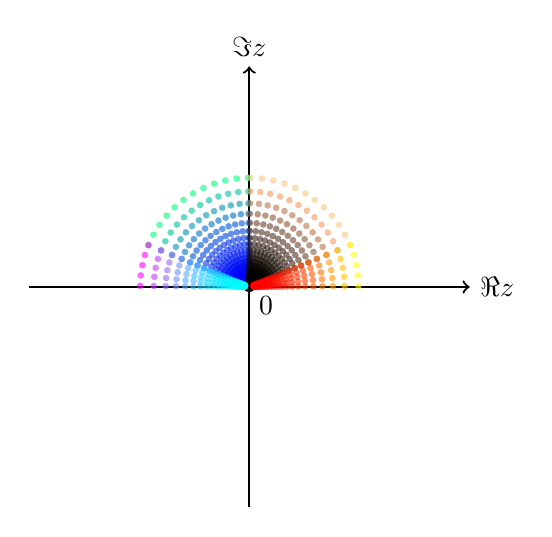
\begin{tikzpicture}[scale=0.8]

\draw[->, thick] (-3.5,0) -- (3.5,0) node[right] {$\Re z$};
\draw[->, thick] (0,-3.5) -- (0,3.5) node[above] {$\Im z$};

\fill (0,0) circle (2.5pt) node[below right] {$0$};

\fill[color={rgb,255:red,0; green,0; blue,255}, opacity=0.60] (-0.0008,0.0808) circle (1.5pt);
\fill[color={rgb,255:red,0; green,0; blue,255}, opacity=0.60] (-0.0009,0.0923) circle (1.5pt);
\fill[color={rgb,255:red,0; green,0; blue,255}, opacity=0.60] (-0.0011,0.1055) circle (1.5pt);
\fill[color={rgb,255:red,0; green,0; blue,255}, opacity=0.60] (-0.0012,0.1205) circle (1.5pt);
\fill[color={rgb,255:red,0; green,1; blue,254}, opacity=0.60] (-0.0014,0.1377) circle (1.5pt);
\fill[color={rgb,255:red,0; green,1; blue,254}, opacity=0.60] (-0.0016,0.1573) circle (1.5pt);
\fill[color={rgb,255:red,0; green,2; blue,254}, opacity=0.60] (-0.0018,0.1797) circle (1.5pt);
\fill[color={rgb,255:red,0; green,3; blue,253}, opacity=0.60] (-0.0021,0.2053) circle (1.5pt);
\fill[color={rgb,255:red,0; green,4; blue,253}, opacity=0.60] (-0.0023,0.2346) circle (1.5pt);
\fill[color={rgb,255:red,0; green,5; blue,252}, opacity=0.60] (-0.0027,0.2681) circle (1.5pt);
\fill[color={rgb,255:red,0; green,7; blue,251}, opacity=0.60] (-0.0031,0.3063) circle (1.5pt);
\fill[color={rgb,255:red,0; green,10; blue,250}, opacity=0.60] (-0.0035,0.3499) circle (1.5pt);
\fill[color={rgb,255:red,0; green,13; blue,248}, opacity=0.60] (-0.0040,0.3998) circle (1.5pt);
\fill[color={rgb,255:red,0; green,17; blue,246}, opacity=0.60] (-0.0046,0.4568) circle (1.5pt);
\fill[color={rgb,255:red,0; green,22; blue,244}, opacity=0.60] (-0.0052,0.5220) circle (1.5pt);
\fill[color={rgb,255:red,0; green,29; blue,240}, opacity=0.60] (-0.0060,0.5964) circle (1.5pt);
\fill[color={rgb,255:red,0; green,39; blue,235}, opacity=0.60] (-0.0068,0.6814) circle (1.5pt);
\fill[color={rgb,255:red,0; green,51; blue,229}, opacity=0.60] (-0.0078,0.7785) circle (1.5pt);
\fill[color={rgb,255:red,0; green,67; blue,221}, opacity=0.60] (-0.0089,0.8895) circle (1.5pt);
\fill[color={rgb,255:red,0; green,87; blue,211}, opacity=0.60] (-0.0102,1.0163) circle (1.5pt);
\fill[color={rgb,255:red,0; green,113; blue,198}, opacity=0.60] (-0.0116,1.1612) circle (1.5pt);
\fill[color={rgb,255:red,0; green,150; blue,179}, opacity=0.60] (-0.0133,1.3267) circle (1.5pt);
\fill[color={rgb,255:red,0; green,195; blue,157}, opacity=0.60] (-0.0152,1.5159) circle (1.5pt);
\fill[color={rgb,255:red,0; green,255; blue,127}, opacity=0.60] (-0.0173,1.7320) circle (1.5pt);
\fill[color={rgb,255:red,0; green,0; blue,255}, opacity=0.60] (-0.0082,0.0702) circle (1.5pt);
\fill[color={rgb,255:red,0; green,0; blue,255}, opacity=0.60] (-0.0094,0.0802) circle (1.5pt);
\fill[color={rgb,255:red,0; green,0; blue,255}, opacity=0.60] (-0.0107,0.0917) circle (1.5pt);
\fill[color={rgb,255:red,0; green,0; blue,255}, opacity=0.60] (-0.0122,0.1048) circle (1.5pt);
\fill[color={rgb,255:red,0; green,0; blue,255}, opacity=0.60] (-0.0140,0.1197) circle (1.5pt);
\fill[color={rgb,255:red,0; green,1; blue,254}, opacity=0.60] (-0.0160,0.1368) circle (1.5pt);
\fill[color={rgb,255:red,0; green,1; blue,254}, opacity=0.60] (-0.0182,0.1562) circle (1.5pt);
\fill[color={rgb,255:red,0; green,2; blue,254}, opacity=0.60] (-0.0208,0.1785) circle (1.5pt);
\fill[color={rgb,255:red,0; green,3; blue,253}, opacity=0.60] (-0.0238,0.2040) circle (1.5pt);
\fill[color={rgb,255:red,0; green,4; blue,253}, opacity=0.60] (-0.0272,0.2331) circle (1.5pt);
\fill[color={rgb,255:red,0; green,5; blue,252}, opacity=0.60] (-0.0311,0.2663) circle (1.5pt);
\fill[color={rgb,255:red,0; green,7; blue,251}, opacity=0.60] (-0.0355,0.3042) circle (1.5pt);
\fill[color={rgb,255:red,0; green,10; blue,250}, opacity=0.60] (-0.0406,0.3476) circle (1.5pt);
\fill[color={rgb,255:red,0; green,13; blue,248}, opacity=0.60] (-0.0464,0.3972) circle (1.5pt);
\fill[color={rgb,255:red,0; green,17; blue,246}, opacity=0.60] (-0.0530,0.4538) circle (1.5pt);
\fill[color={rgb,255:red,0; green,22; blue,244}, opacity=0.60] (-0.0605,0.5185) circle (1.5pt);
\fill[color={rgb,255:red,0; green,29; blue,240}, opacity=0.60] (-0.0691,0.5924) circle (1.5pt);
\fill[color={rgb,255:red,0; green,39; blue,235}, opacity=0.60] (-0.0790,0.6768) circle (1.5pt);
\fill[color={rgb,255:red,0; green,51; blue,229}, opacity=0.60] (-0.0903,0.7733) circle (1.5pt);
\fill[color={rgb,255:red,0; green,67; blue,221}, opacity=0.60] (-0.1031,0.8836) circle (1.5pt);
\fill[color={rgb,255:red,0; green,87; blue,211}, opacity=0.60] (-0.1178,1.0095) circle (1.5pt);
\fill[color={rgb,255:red,0; green,113; blue,198}, opacity=0.60] (-0.1346,1.1534) circle (1.5pt);
\fill[color={rgb,255:red,0; green,150; blue,179}, opacity=0.60] (-0.1538,1.3179) circle (1.5pt);
\fill[color={rgb,255:red,0; green,195; blue,157}, opacity=0.60] (-0.1757,1.5057) circle (1.5pt);
\fill[color={rgb,255:red,0; green,255; blue,127}, opacity=0.60] (-0.2008,1.7204) circle (1.5pt);
\fill[color={rgb,255:red,0; green,0; blue,255}, opacity=0.60] (-0.0156,0.0690) circle (1.5pt);
\fill[color={rgb,255:red,0; green,0; blue,255}, opacity=0.60] (-0.0178,0.0788) circle (1.5pt);
\fill[color={rgb,255:red,0; green,0; blue,255}, opacity=0.60] (-0.0204,0.0900) circle (1.5pt);
\fill[color={rgb,255:red,0; green,0; blue,255}, opacity=0.60] (-0.0233,0.1029) circle (1.5pt);
\fill[color={rgb,255:red,0; green,0; blue,255}, opacity=0.60] (-0.0266,0.1175) circle (1.5pt);
\fill[color={rgb,255:red,0; green,1; blue,254}, opacity=0.60] (-0.0304,0.1343) circle (1.5pt);
\fill[color={rgb,255:red,0; green,1; blue,254}, opacity=0.60] (-0.0347,0.1534) circle (1.5pt);
\fill[color={rgb,255:red,0; green,2; blue,254}, opacity=0.60] (-0.0396,0.1753) circle (1.5pt);
\fill[color={rgb,255:red,0; green,3; blue,253}, opacity=0.60] (-0.0453,0.2003) circle (1.5pt);
\fill[color={rgb,255:red,0; green,4; blue,253}, opacity=0.60] (-0.0517,0.2289) circle (1.5pt);
\fill[color={rgb,255:red,0; green,5; blue,252}, opacity=0.60] (-0.0591,0.2615) circle (1.5pt);
\fill[color={rgb,255:red,0; green,7; blue,251}, opacity=0.60] (-0.0676,0.2988) circle (1.5pt);
\fill[color={rgb,255:red,0; green,10; blue,250}, opacity=0.60] (-0.0772,0.3413) circle (1.5pt);
\fill[color={rgb,255:red,0; green,13; blue,248}, opacity=0.60] (-0.0882,0.3900) circle (1.5pt);
\fill[color={rgb,255:red,0; green,17; blue,246}, opacity=0.60] (-0.1008,0.4456) circle (1.5pt);
\fill[color={rgb,255:red,0; green,22; blue,244}, opacity=0.60] (-0.1151,0.5091) circle (1.5pt);
\fill[color={rgb,255:red,0; green,29; blue,240}, opacity=0.60] (-0.1315,0.5817) circle (1.5pt);
\fill[color={rgb,255:red,0; green,39; blue,235}, opacity=0.60] (-0.1503,0.6646) circle (1.5pt);
\fill[color={rgb,255:red,0; green,51; blue,229}, opacity=0.60] (-0.1717,0.7594) circle (1.5pt);
\fill[color={rgb,255:red,0; green,67; blue,221}, opacity=0.60] (-0.1962,0.8676) circle (1.5pt);
\fill[color={rgb,255:red,0; green,87; blue,211}, opacity=0.60] (-0.2242,0.9913) circle (1.5pt);
\fill[color={rgb,255:red,0; green,113; blue,198}, opacity=0.60] (-0.2561,1.1327) circle (1.5pt);
\fill[color={rgb,255:red,0; green,150; blue,179}, opacity=0.60] (-0.2926,1.2941) circle (1.5pt);
\fill[color={rgb,255:red,0; green,195; blue,157}, opacity=0.60] (-0.3343,1.4786) circle (1.5pt);
\fill[color={rgb,255:red,0; green,255; blue,127}, opacity=0.60] (-0.3820,1.6894) circle (1.5pt);
\fill[color={rgb,255:red,0; green,0; blue,255}, opacity=0.60] (-0.0228,0.0669) circle (1.5pt);
\fill[color={rgb,255:red,0; green,0; blue,255}, opacity=0.60] (-0.0261,0.0765) circle (1.5pt);
\fill[color={rgb,255:red,0; green,0; blue,255}, opacity=0.60] (-0.0298,0.0874) circle (1.5pt);
\fill[color={rgb,255:red,0; green,0; blue,255}, opacity=0.60] (-0.0340,0.0998) circle (1.5pt);
\fill[color={rgb,255:red,0; green,0; blue,255}, opacity=0.60] (-0.0389,0.1141) circle (1.5pt);
\fill[color={rgb,255:red,0; green,1; blue,254}, opacity=0.60] (-0.0444,0.1303) circle (1.5pt);
\fill[color={rgb,255:red,0; green,1; blue,254}, opacity=0.60] (-0.0508,0.1489) circle (1.5pt);
\fill[color={rgb,255:red,0; green,2; blue,254}, opacity=0.60] (-0.0580,0.1701) circle (1.5pt);
\fill[color={rgb,255:red,0; green,3; blue,253}, opacity=0.60] (-0.0663,0.1944) circle (1.5pt);
\fill[color={rgb,255:red,0; green,4; blue,253}, opacity=0.60] (-0.0757,0.2221) circle (1.5pt);
\fill[color={rgb,255:red,0; green,5; blue,252}, opacity=0.60] (-0.0865,0.2537) circle (1.5pt);
\fill[color={rgb,255:red,0; green,7; blue,251}, opacity=0.60] (-0.0988,0.2899) circle (1.5pt);
\fill[color={rgb,255:red,0; green,10; blue,250}, opacity=0.60] (-0.1129,0.3312) circle (1.5pt);
\fill[color={rgb,255:red,0; green,13; blue,248}, opacity=0.60] (-0.1290,0.3785) circle (1.5pt);
\fill[color={rgb,255:red,0; green,17; blue,246}, opacity=0.60] (-0.1474,0.4324) circle (1.5pt);
\fill[color={rgb,255:red,0; green,22; blue,244}, opacity=0.60] (-0.1684,0.4941) circle (1.5pt);
\fill[color={rgb,255:red,0; green,29; blue,240}, opacity=0.60] (-0.1925,0.5645) circle (1.5pt);
\fill[color={rgb,255:red,0; green,39; blue,235}, opacity=0.60] (-0.2199,0.6450) circle (1.5pt);
\fill[color={rgb,255:red,0; green,51; blue,229}, opacity=0.60] (-0.2512,0.7369) circle (1.5pt);
\fill[color={rgb,255:red,0; green,67; blue,221}, opacity=0.60] (-0.2871,0.8420) circle (1.5pt);
\fill[color={rgb,255:red,0; green,87; blue,211}, opacity=0.60] (-0.3280,0.9620) circle (1.5pt);
\fill[color={rgb,255:red,0; green,113; blue,198}, opacity=0.60] (-0.3747,1.0991) circle (1.5pt);
\fill[color={rgb,255:red,0; green,150; blue,179}, opacity=0.60] (-0.4281,1.2558) circle (1.5pt);
\fill[color={rgb,255:red,0; green,195; blue,157}, opacity=0.60] (-0.4892,1.4348) circle (1.5pt);
\fill[color={rgb,255:red,0; green,255; blue,127}, opacity=0.60] (-0.5589,1.6394) circle (1.5pt);
\fill[color={rgb,255:red,0; green,0; blue,255}, opacity=0.60] (-0.0298,0.0641) circle (1.5pt);
\fill[color={rgb,255:red,0; green,0; blue,255}, opacity=0.60] (-0.0340,0.0733) circle (1.5pt);
\fill[color={rgb,255:red,0; green,0; blue,255}, opacity=0.60] (-0.0389,0.0837) circle (1.5pt);
\fill[color={rgb,255:red,0; green,0; blue,255}, opacity=0.60] (-0.0444,0.0957) circle (1.5pt);
\fill[color={rgb,255:red,0; green,0; blue,255}, opacity=0.60] (-0.0508,0.1093) circle (1.5pt);
\fill[color={rgb,255:red,0; green,1; blue,254}, opacity=0.60] (-0.0580,0.1249) circle (1.5pt);
\fill[color={rgb,255:red,0; green,1; blue,254}, opacity=0.60] (-0.0663,0.1427) circle (1.5pt);
\fill[color={rgb,255:red,0; green,2; blue,254}, opacity=0.60] (-0.0757,0.1630) circle (1.5pt);
\fill[color={rgb,255:red,0; green,3; blue,253}, opacity=0.60] (-0.0865,0.1863) circle (1.5pt);
\fill[color={rgb,255:red,0; green,4; blue,253}, opacity=0.60] (-0.0988,0.2128) circle (1.5pt);
\fill[color={rgb,255:red,0; green,5; blue,252}, opacity=0.60] (-0.1129,0.2431) circle (1.5pt);
\fill[color={rgb,255:red,0; green,7; blue,251}, opacity=0.60] (-0.1290,0.2778) circle (1.5pt);
\fill[color={rgb,255:red,0; green,10; blue,250}, opacity=0.60] (-0.1474,0.3174) circle (1.5pt);
\fill[color={rgb,255:red,0; green,13; blue,248}, opacity=0.60] (-0.1684,0.3627) circle (1.5pt);
\fill[color={rgb,255:red,0; green,17; blue,246}, opacity=0.60] (-0.1924,0.4144) circle (1.5pt);
\fill[color={rgb,255:red,0; green,22; blue,244}, opacity=0.60] (-0.2199,0.4734) circle (1.5pt);
\fill[color={rgb,255:red,0; green,29; blue,240}, opacity=0.60] (-0.2512,0.5409) circle (1.5pt);
\fill[color={rgb,255:red,0; green,39; blue,235}, opacity=0.60] (-0.2870,0.6180) circle (1.5pt);
\fill[color={rgb,255:red,0; green,51; blue,229}, opacity=0.60] (-0.3279,0.7061) circle (1.5pt);
\fill[color={rgb,255:red,0; green,67; blue,221}, opacity=0.60] (-0.3747,0.8068) circle (1.5pt);
\fill[color={rgb,255:red,0; green,87; blue,211}, opacity=0.60] (-0.4281,0.9218) circle (1.5pt);
\fill[color={rgb,255:red,0; green,113; blue,198}, opacity=0.60] (-0.4891,1.0532) circle (1.5pt);
\fill[color={rgb,255:red,0; green,150; blue,179}, opacity=0.60] (-0.5588,1.2034) circle (1.5pt);
\fill[color={rgb,255:red,0; green,195; blue,157}, opacity=0.60] (-0.6385,1.3749) circle (1.5pt);
\fill[color={rgb,255:red,0; green,255; blue,127}, opacity=0.60] (-0.7295,1.5709) circle (1.5pt);
\fill[color={rgb,255:red,0; green,0; blue,255}, opacity=0.60] (-0.0364,0.0606) circle (1.5pt);
\fill[color={rgb,255:red,0; green,0; blue,255}, opacity=0.60] (-0.0416,0.0693) circle (1.5pt);
\fill[color={rgb,255:red,0; green,0; blue,255}, opacity=0.60] (-0.0475,0.0791) circle (1.5pt);
\fill[color={rgb,255:red,0; green,0; blue,255}, opacity=0.60] (-0.0543,0.0904) circle (1.5pt);
\fill[color={rgb,255:red,0; green,0; blue,255}, opacity=0.60] (-0.0621,0.1033) circle (1.5pt);
\fill[color={rgb,255:red,0; green,1; blue,254}, opacity=0.60] (-0.0709,0.1180) circle (1.5pt);
\fill[color={rgb,255:red,0; green,1; blue,254}, opacity=0.60] (-0.0810,0.1348) circle (1.5pt);
\fill[color={rgb,255:red,0; green,2; blue,254}, opacity=0.60] (-0.0926,0.1541) circle (1.5pt);
\fill[color={rgb,255:red,0; green,3; blue,253}, opacity=0.60] (-0.1057,0.1760) circle (1.5pt);
\fill[color={rgb,255:red,0; green,4; blue,253}, opacity=0.60] (-0.1208,0.2011) circle (1.5pt);
\fill[color={rgb,255:red,0; green,5; blue,252}, opacity=0.60] (-0.1380,0.2298) circle (1.5pt);
\fill[color={rgb,255:red,0; green,7; blue,251}, opacity=0.60] (-0.1577,0.2626) circle (1.5pt);
\fill[color={rgb,255:red,0; green,10; blue,250}, opacity=0.60] (-0.1802,0.3000) circle (1.5pt);
\fill[color={rgb,255:red,0; green,13; blue,248}, opacity=0.60] (-0.2059,0.3428) circle (1.5pt);
\fill[color={rgb,255:red,0; green,17; blue,246}, opacity=0.60] (-0.2353,0.3916) circle (1.5pt);
\fill[color={rgb,255:red,0; green,22; blue,244}, opacity=0.60] (-0.2688,0.4475) circle (1.5pt);
\fill[color={rgb,255:red,0; green,29; blue,240}, opacity=0.60] (-0.3071,0.5112) circle (1.5pt);
\fill[color={rgb,255:red,0; green,39; blue,235}, opacity=0.60] (-0.3509,0.5841) circle (1.5pt);
\fill[color={rgb,255:red,0; green,51; blue,229}, opacity=0.60] (-0.4009,0.6674) circle (1.5pt);
\fill[color={rgb,255:red,0; green,67; blue,221}, opacity=0.60] (-0.4581,0.7625) circle (1.5pt);
\fill[color={rgb,255:red,0; green,87; blue,211}, opacity=0.60] (-0.5234,0.8712) circle (1.5pt);
\fill[color={rgb,255:red,0; green,113; blue,198}, opacity=0.60] (-0.5980,0.9954) circle (1.5pt);
\fill[color={rgb,255:red,0; green,150; blue,179}, opacity=0.60] (-0.6832,1.1374) circle (1.5pt);
\fill[color={rgb,255:red,0; green,195; blue,157}, opacity=0.60] (-0.7806,1.2995) circle (1.5pt);
\fill[color={rgb,255:red,0; green,255; blue,127}, opacity=0.60] (-0.8919,1.4847) circle (1.5pt);
\fill[color={rgb,255:red,0; green,0; blue,255}, opacity=0.60] (-0.0426,0.0564) circle (1.5pt);
\fill[color={rgb,255:red,0; green,0; blue,255}, opacity=0.60] (-0.0487,0.0645) circle (1.5pt);
\fill[color={rgb,255:red,0; green,0; blue,255}, opacity=0.60] (-0.0557,0.0736) circle (1.5pt);
\fill[color={rgb,255:red,0; green,0; blue,255}, opacity=0.60] (-0.0636,0.0841) circle (1.5pt);
\fill[color={rgb,255:red,0; green,0; blue,255}, opacity=0.60] (-0.0727,0.0961) circle (1.5pt);
\fill[color={rgb,255:red,0; green,1; blue,254}, opacity=0.60] (-0.0830,0.1098) circle (1.5pt);
\fill[color={rgb,255:red,0; green,1; blue,254}, opacity=0.60] (-0.0948,0.1255) circle (1.5pt);
\fill[color={rgb,255:red,0; green,2; blue,254}, opacity=0.60] (-0.1084,0.1434) circle (1.5pt);
\fill[color={rgb,255:red,0; green,3; blue,253}, opacity=0.60] (-0.1238,0.1638) circle (1.5pt);
\fill[color={rgb,255:red,0; green,4; blue,253}, opacity=0.60] (-0.1415,0.1872) circle (1.5pt);
\fill[color={rgb,255:red,0; green,5; blue,252}, opacity=0.60] (-0.1616,0.2139) circle (1.5pt);
\fill[color={rgb,255:red,0; green,7; blue,251}, opacity=0.60] (-0.1847,0.2444) circle (1.5pt);
\fill[color={rgb,255:red,0; green,10; blue,250}, opacity=0.60] (-0.2110,0.2792) circle (1.5pt);
\fill[color={rgb,255:red,0; green,13; blue,248}, opacity=0.60] (-0.2411,0.3190) circle (1.5pt);
\fill[color={rgb,255:red,0; green,17; blue,246}, opacity=0.60] (-0.2754,0.3645) circle (1.5pt);
\fill[color={rgb,255:red,0; green,22; blue,244}, opacity=0.60] (-0.3147,0.4164) circle (1.5pt);
\fill[color={rgb,255:red,0; green,29; blue,240}, opacity=0.60] (-0.3596,0.4758) circle (1.5pt);
\fill[color={rgb,255:red,0; green,39; blue,235}, opacity=0.60] (-0.4108,0.5436) circle (1.5pt);
\fill[color={rgb,255:red,0; green,51; blue,229}, opacity=0.60] (-0.4694,0.6211) circle (1.5pt);
\fill[color={rgb,255:red,0; green,67; blue,221}, opacity=0.60] (-0.5363,0.7097) circle (1.5pt);
\fill[color={rgb,255:red,0; green,87; blue,211}, opacity=0.60] (-0.6128,0.8109) circle (1.5pt);
\fill[color={rgb,255:red,0; green,113; blue,198}, opacity=0.60] (-0.7001,0.9265) circle (1.5pt);
\fill[color={rgb,255:red,0; green,150; blue,179}, opacity=0.60] (-0.7999,1.0585) circle (1.5pt);
\fill[color={rgb,255:red,0; green,195; blue,157}, opacity=0.60] (-0.9140,1.2094) circle (1.5pt);
\fill[color={rgb,255:red,0; green,255; blue,127}, opacity=0.60] (-1.0443,1.3818) circle (1.5pt);
\fill[color={rgb,255:red,0; green,0; blue,255}, opacity=0.60] (-0.0484,0.0516) circle (1.5pt);
\fill[color={rgb,255:red,0; green,0; blue,255}, opacity=0.60] (-0.0553,0.0589) circle (1.5pt);
\fill[color={rgb,255:red,0; green,0; blue,255}, opacity=0.60] (-0.0631,0.0673) circle (1.5pt);
\fill[color={rgb,255:red,0; green,0; blue,255}, opacity=0.60] (-0.0721,0.0769) circle (1.5pt);
\fill[color={rgb,255:red,0; green,0; blue,255}, opacity=0.60] (-0.0824,0.0879) circle (1.5pt);
\fill[color={rgb,255:red,0; green,1; blue,254}, opacity=0.60] (-0.0942,0.1004) circle (1.5pt);
\fill[color={rgb,255:red,0; green,1; blue,254}, opacity=0.60] (-0.1076,0.1147) circle (1.5pt);
\fill[color={rgb,255:red,0; green,2; blue,254}, opacity=0.60] (-0.1230,0.1311) circle (1.5pt);
\fill[color={rgb,255:red,0; green,3; blue,253}, opacity=0.60] (-0.1405,0.1498) circle (1.5pt);
\fill[color={rgb,255:red,0; green,4; blue,253}, opacity=0.60] (-0.1605,0.1711) circle (1.5pt);
\fill[color={rgb,255:red,0; green,5; blue,252}, opacity=0.60] (-0.1834,0.1955) circle (1.5pt);
\fill[color={rgb,255:red,0; green,7; blue,251}, opacity=0.60] (-0.2095,0.2234) circle (1.5pt);
\fill[color={rgb,255:red,0; green,10; blue,250}, opacity=0.60] (-0.2394,0.2553) circle (1.5pt);
\fill[color={rgb,255:red,0; green,13; blue,248}, opacity=0.60] (-0.2735,0.2917) circle (1.5pt);
\fill[color={rgb,255:red,0; green,17; blue,246}, opacity=0.60] (-0.3125,0.3332) circle (1.5pt);
\fill[color={rgb,255:red,0; green,22; blue,244}, opacity=0.60] (-0.3571,0.3807) circle (1.5pt);
\fill[color={rgb,255:red,0; green,29; blue,240}, opacity=0.60] (-0.4080,0.4350) circle (1.5pt);
\fill[color={rgb,255:red,0; green,39; blue,235}, opacity=0.60] (-0.4661,0.4970) circle (1.5pt);
\fill[color={rgb,255:red,0; green,51; blue,229}, opacity=0.60] (-0.5326,0.5679) circle (1.5pt);
\fill[color={rgb,255:red,0; green,67; blue,221}, opacity=0.60] (-0.6085,0.6488) circle (1.5pt);
\fill[color={rgb,255:red,0; green,87; blue,211}, opacity=0.60] (-0.6953,0.7413) circle (1.5pt);
\fill[color={rgb,255:red,0; green,113; blue,198}, opacity=0.60] (-0.7944,0.8470) circle (1.5pt);
\fill[color={rgb,255:red,0; green,150; blue,179}, opacity=0.60] (-0.9076,0.9678) circle (1.5pt);
\fill[color={rgb,255:red,0; green,195; blue,157}, opacity=0.60] (-1.0370,1.1057) circle (1.5pt);
\fill[color={rgb,255:red,0; green,255; blue,127}, opacity=0.60] (-1.1849,1.2634) circle (1.5pt);
\fill[color={rgb,255:red,0; green,0; blue,255}, opacity=0.60] (-0.0536,0.0462) circle (1.5pt);
\fill[color={rgb,255:red,0; green,0; blue,255}, opacity=0.60] (-0.0612,0.0527) circle (1.5pt);
\fill[color={rgb,255:red,0; green,0; blue,255}, opacity=0.60] (-0.0699,0.0603) circle (1.5pt);
\fill[color={rgb,255:red,0; green,0; blue,255}, opacity=0.60] (-0.0799,0.0688) circle (1.5pt);
\fill[color={rgb,255:red,0; green,0; blue,255}, opacity=0.60] (-0.0913,0.0787) circle (1.5pt);
\fill[color={rgb,255:red,0; green,1; blue,254}, opacity=0.60] (-0.1043,0.0899) circle (1.5pt);
\fill[color={rgb,255:red,0; green,1; blue,254}, opacity=0.60] (-0.1192,0.1027) circle (1.5pt);
\fill[color={rgb,255:red,0; green,2; blue,254}, opacity=0.60] (-0.1362,0.1173) circle (1.5pt);
\fill[color={rgb,255:red,0; green,3; blue,253}, opacity=0.60] (-0.1556,0.1341) circle (1.5pt);
\fill[color={rgb,255:red,0; green,4; blue,253}, opacity=0.60] (-0.1777,0.1532) circle (1.5pt);
\fill[color={rgb,255:red,0; green,5; blue,252}, opacity=0.60] (-0.2031,0.1750) circle (1.5pt);
\fill[color={rgb,255:red,0; green,7; blue,251}, opacity=0.60] (-0.2320,0.2000) circle (1.5pt);
\fill[color={rgb,255:red,0; green,10; blue,250}, opacity=0.60] (-0.2651,0.2285) circle (1.5pt);
\fill[color={rgb,255:red,0; green,13; blue,248}, opacity=0.60] (-0.3029,0.2610) circle (1.5pt);
\fill[color={rgb,255:red,0; green,17; blue,246}, opacity=0.60] (-0.3461,0.2982) circle (1.5pt);
\fill[color={rgb,255:red,0; green,22; blue,244}, opacity=0.60] (-0.3954,0.3407) circle (1.5pt);
\fill[color={rgb,255:red,0; green,29; blue,240}, opacity=0.60] (-0.4518,0.3893) circle (1.5pt);
\fill[color={rgb,255:red,0; green,39; blue,235}, opacity=0.60] (-0.5162,0.4448) circle (1.5pt);
\fill[color={rgb,255:red,0; green,51; blue,229}, opacity=0.60] (-0.5898,0.5082) circle (1.5pt);
\fill[color={rgb,255:red,0; green,67; blue,221}, opacity=0.60] (-0.6739,0.5807) circle (1.5pt);
\fill[color={rgb,255:red,0; green,87; blue,211}, opacity=0.60] (-0.7699,0.6635) circle (1.5pt);
\fill[color={rgb,255:red,0; green,113; blue,198}, opacity=0.60] (-0.8797,0.7581) circle (1.5pt);
\fill[color={rgb,255:red,0; green,150; blue,179}, opacity=0.60] (-1.0051,0.8661) circle (1.5pt);
\fill[color={rgb,255:red,0; green,195; blue,157}, opacity=0.60] (-1.1484,0.9896) circle (1.5pt);
\fill[color={rgb,255:red,0; green,255; blue,127}, opacity=0.60] (-1.3121,1.1307) circle (1.5pt);
\fill[color={rgb,255:red,0; green,0; blue,255}, opacity=0.60] (-0.0582,0.0402) circle (1.5pt);
\fill[color={rgb,255:red,0; green,0; blue,255}, opacity=0.60] (-0.0664,0.0460) circle (1.5pt);
\fill[color={rgb,255:red,0; green,0; blue,255}, opacity=0.60] (-0.0759,0.0525) circle (1.5pt);
\fill[color={rgb,255:red,0; green,0; blue,255}, opacity=0.60] (-0.0867,0.0600) circle (1.5pt);
\fill[color={rgb,255:red,0; green,0; blue,255}, opacity=0.60] (-0.0991,0.0685) circle (1.5pt);
\fill[color={rgb,255:red,0; green,1; blue,254}, opacity=0.60] (-0.1132,0.0783) circle (1.5pt);
\fill[color={rgb,255:red,0; green,1; blue,254}, opacity=0.60] (-0.1294,0.0895) circle (1.5pt);
\fill[color={rgb,255:red,0; green,2; blue,254}, opacity=0.60] (-0.1478,0.1022) circle (1.5pt);
\fill[color={rgb,255:red,0; green,3; blue,253}, opacity=0.60] (-0.1689,0.1168) circle (1.5pt);
\fill[color={rgb,255:red,0; green,4; blue,253}, opacity=0.60] (-0.1930,0.1335) circle (1.5pt);
\fill[color={rgb,255:red,0; green,5; blue,252}, opacity=0.60] (-0.2205,0.1525) circle (1.5pt);
\fill[color={rgb,255:red,0; green,7; blue,251}, opacity=0.60] (-0.2519,0.1742) circle (1.5pt);
\fill[color={rgb,255:red,0; green,10; blue,250}, opacity=0.60] (-0.2878,0.1991) circle (1.5pt);
\fill[color={rgb,255:red,0; green,13; blue,248}, opacity=0.60] (-0.3289,0.2274) circle (1.5pt);
\fill[color={rgb,255:red,0; green,17; blue,246}, opacity=0.60] (-0.3757,0.2599) circle (1.5pt);
\fill[color={rgb,255:red,0; green,22; blue,244}, opacity=0.60] (-0.4293,0.2969) circle (1.5pt);
\fill[color={rgb,255:red,0; green,29; blue,240}, opacity=0.60] (-0.4905,0.3392) circle (1.5pt);
\fill[color={rgb,255:red,0; green,39; blue,235}, opacity=0.60] (-0.5604,0.3876) circle (1.5pt);
\fill[color={rgb,255:red,0; green,51; blue,229}, opacity=0.60] (-0.6403,0.4429) circle (1.5pt);
\fill[color={rgb,255:red,0; green,67; blue,221}, opacity=0.60] (-0.7316,0.5060) circle (1.5pt);
\fill[color={rgb,255:red,0; green,87; blue,211}, opacity=0.60] (-0.8359,0.5781) circle (1.5pt);
\fill[color={rgb,255:red,0; green,113; blue,198}, opacity=0.60] (-0.9551,0.6606) circle (1.5pt);
\fill[color={rgb,255:red,0; green,150; blue,179}, opacity=0.60] (-1.0912,0.7547) circle (1.5pt);
\fill[color={rgb,255:red,0; green,195; blue,157}, opacity=0.60] (-1.2468,0.8623) circle (1.5pt);
\fill[color={rgb,255:red,0; green,255; blue,127}, opacity=0.60] (-1.4245,0.9852) circle (1.5pt);
\fill[color={rgb,255:red,0; green,0; blue,255}, opacity=0.60] (-0.0621,0.0338) circle (1.5pt);
\fill[color={rgb,255:red,0; green,0; blue,255}, opacity=0.60] (-0.0709,0.0387) circle (1.5pt);
\fill[color={rgb,255:red,0; green,0; blue,255}, opacity=0.60] (-0.0811,0.0442) circle (1.5pt);
\fill[color={rgb,255:red,0; green,0; blue,255}, opacity=0.60] (-0.0926,0.0505) circle (1.5pt);
\fill[color={rgb,255:red,0; green,0; blue,255}, opacity=0.60] (-0.1058,0.0577) circle (1.5pt);
\fill[color={rgb,255:red,0; green,1; blue,254}, opacity=0.60] (-0.1209,0.0659) circle (1.5pt);
\fill[color={rgb,255:red,0; green,1; blue,254}, opacity=0.60] (-0.1381,0.0753) circle (1.5pt);
\fill[color={rgb,255:red,0; green,2; blue,254}, opacity=0.60] (-0.1578,0.0860) circle (1.5pt);
\fill[color={rgb,255:red,0; green,3; blue,253}, opacity=0.60] (-0.1803,0.0983) circle (1.5pt);
\fill[color={rgb,255:red,0; green,4; blue,253}, opacity=0.60] (-0.2060,0.1123) circle (1.5pt);
\fill[color={rgb,255:red,0; green,5; blue,252}, opacity=0.60] (-0.2354,0.1283) circle (1.5pt);
\fill[color={rgb,255:red,0; green,7; blue,251}, opacity=0.60] (-0.2690,0.1465) circle (1.5pt);
\fill[color={rgb,255:red,0; green,10; blue,250}, opacity=0.60] (-0.3073,0.1674) circle (1.5pt);
\fill[color={rgb,255:red,0; green,13; blue,248}, opacity=0.60] (-0.3511,0.1913) circle (1.5pt);
\fill[color={rgb,255:red,0; green,17; blue,246}, opacity=0.60] (-0.4012,0.2186) circle (1.5pt);
\fill[color={rgb,255:red,0; green,22; blue,244}, opacity=0.60] (-0.4584,0.2497) circle (1.5pt);
\fill[color={rgb,255:red,0; green,29; blue,240}, opacity=0.60] (-0.5237,0.2853) circle (1.5pt);
\fill[color={rgb,255:red,0; green,39; blue,235}, opacity=0.60] (-0.5984,0.3260) circle (1.5pt);
\fill[color={rgb,255:red,0; green,51; blue,229}, opacity=0.60] (-0.6837,0.3725) circle (1.5pt);
\fill[color={rgb,255:red,0; green,67; blue,221}, opacity=0.60] (-0.7811,0.4256) circle (1.5pt);
\fill[color={rgb,255:red,0; green,87; blue,211}, opacity=0.60] (-0.8925,0.4863) circle (1.5pt);
\fill[color={rgb,255:red,0; green,113; blue,198}, opacity=0.60] (-1.0197,0.5556) circle (1.5pt);
\fill[color={rgb,255:red,0; green,150; blue,179}, opacity=0.60] (-1.1651,0.6348) circle (1.5pt);
\fill[color={rgb,255:red,0; green,195; blue,157}, opacity=0.60] (-1.3312,0.7253) circle (1.5pt);
\fill[color={rgb,255:red,0; green,255; blue,127}, opacity=0.60] (-1.5209,0.8287) circle (1.5pt);
\fill[color={rgb,255:red,0; green,0; blue,255}, opacity=0.60] (-0.0653,0.0271) circle (1.5pt);
\fill[color={rgb,255:red,0; green,0; blue,255}, opacity=0.60] (-0.0746,0.0309) circle (1.5pt);
\fill[color={rgb,255:red,0; green,0; blue,255}, opacity=0.60] (-0.0853,0.0353) circle (1.5pt);
\fill[color={rgb,255:red,0; green,0; blue,255}, opacity=0.60] (-0.0974,0.0404) circle (1.5pt);
\fill[color={rgb,255:red,0; green,0; blue,255}, opacity=0.60] (-0.1113,0.0461) circle (1.5pt);
\fill[color={rgb,255:red,0; green,1; blue,254}, opacity=0.60] (-0.1272,0.0527) circle (1.5pt);
\fill[color={rgb,255:red,0; green,1; blue,254}, opacity=0.60] (-0.1453,0.0602) circle (1.5pt);
\fill[color={rgb,255:red,0; green,2; blue,254}, opacity=0.60] (-0.1661,0.0688) circle (1.5pt);
\fill[color={rgb,255:red,0; green,3; blue,253}, opacity=0.60] (-0.1897,0.0786) circle (1.5pt);
\fill[color={rgb,255:red,0; green,4; blue,253}, opacity=0.60] (-0.2168,0.0898) circle (1.5pt);
\fill[color={rgb,255:red,0; green,5; blue,252}, opacity=0.60] (-0.2477,0.1026) circle (1.5pt);
\fill[color={rgb,255:red,0; green,7; blue,251}, opacity=0.60] (-0.2830,0.1172) circle (1.5pt);
\fill[color={rgb,255:red,0; green,10; blue,250}, opacity=0.60] (-0.3233,0.1339) circle (1.5pt);
\fill[color={rgb,255:red,0; green,13; blue,248}, opacity=0.60] (-0.3694,0.1530) circle (1.5pt);
\fill[color={rgb,255:red,0; green,17; blue,246}, opacity=0.60] (-0.4221,0.1748) circle (1.5pt);
\fill[color={rgb,255:red,0; green,22; blue,244}, opacity=0.60] (-0.4823,0.1998) circle (1.5pt);
\fill[color={rgb,255:red,0; green,29; blue,240}, opacity=0.60] (-0.5510,0.2282) circle (1.5pt);
\fill[color={rgb,255:red,0; green,39; blue,235}, opacity=0.60] (-0.6295,0.2608) circle (1.5pt);
\fill[color={rgb,255:red,0; green,51; blue,229}, opacity=0.60] (-0.7193,0.2979) circle (1.5pt);
\fill[color={rgb,255:red,0; green,67; blue,221}, opacity=0.60] (-0.8218,0.3404) circle (1.5pt);
\fill[color={rgb,255:red,0; green,87; blue,211}, opacity=0.60] (-0.9390,0.3889) circle (1.5pt);
\fill[color={rgb,255:red,0; green,113; blue,198}, opacity=0.60] (-1.0729,0.4444) circle (1.5pt);
\fill[color={rgb,255:red,0; green,150; blue,179}, opacity=0.60] (-1.2258,0.5077) circle (1.5pt);
\fill[color={rgb,255:red,0; green,195; blue,157}, opacity=0.60] (-1.4005,0.5801) circle (1.5pt);
\fill[color={rgb,255:red,0; green,255; blue,127}, opacity=0.60] (-1.6002,0.6628) circle (1.5pt);
\fill[color={rgb,255:red,0; green,0; blue,0}, opacity=0.60] (0.0653,0.0271) circle (1.5pt);
\fill[color={rgb,255:red,0; green,0; blue,0}, opacity=0.60] (0.0746,0.0309) circle (1.5pt);
\fill[color={rgb,255:red,0; green,0; blue,0}, opacity=0.60] (0.0853,0.0353) circle (1.5pt);
\fill[color={rgb,255:red,0; green,0; blue,0}, opacity=0.60] (0.0974,0.0404) circle (1.5pt);
\fill[color={rgb,255:red,0; green,0; blue,0}, opacity=0.60] (0.1113,0.0461) circle (1.5pt);
\fill[color={rgb,255:red,1; green,0; blue,0}, opacity=0.60] (0.1272,0.0527) circle (1.5pt);
\fill[color={rgb,255:red,1; green,0; blue,0}, opacity=0.60] (0.1453,0.0602) circle (1.5pt);
\fill[color={rgb,255:red,2; green,1; blue,0}, opacity=0.60] (0.1661,0.0688) circle (1.5pt);
\fill[color={rgb,255:red,3; green,2; blue,1}, opacity=0.60] (0.1897,0.0786) circle (1.5pt);
\fill[color={rgb,255:red,4; green,3; blue,1}, opacity=0.60] (0.2168,0.0898) circle (1.5pt);
\fill[color={rgb,255:red,6; green,3; blue,2}, opacity=0.60] (0.2477,0.1026) circle (1.5pt);
\fill[color={rgb,255:red,8; green,5; blue,3}, opacity=0.60] (0.2830,0.1172) circle (1.5pt);
\fill[color={rgb,255:red,12; green,7; blue,4}, opacity=0.60] (0.3233,0.1339) circle (1.5pt);
\fill[color={rgb,255:red,16; green,10; blue,6}, opacity=0.60] (0.3694,0.1530) circle (1.5pt);
\fill[color={rgb,255:red,20; green,13; blue,8}, opacity=0.60] (0.4221,0.1748) circle (1.5pt);
\fill[color={rgb,255:red,27; green,17; blue,10}, opacity=0.60] (0.4823,0.1998) circle (1.5pt);
\fill[color={rgb,255:red,35; green,22; blue,14}, opacity=0.60] (0.5510,0.2282) circle (1.5pt);
\fill[color={rgb,255:red,48; green,30; blue,19}, opacity=0.60] (0.6295,0.2608) circle (1.5pt);
\fill[color={rgb,255:red,62; green,39; blue,25}, opacity=0.60] (0.7193,0.2979) circle (1.5pt);
\fill[color={rgb,255:red,82; green,52; blue,33}, opacity=0.60] (0.8218,0.3404) circle (1.5pt);
\fill[color={rgb,255:red,107; green,67; blue,43}, opacity=0.60] (0.9390,0.3889) circle (1.5pt);
\fill[color={rgb,255:red,140; green,89; blue,56}, opacity=0.60] (1.0729,0.4444) circle (1.5pt);
\fill[color={rgb,255:red,185; green,117; blue,74}, opacity=0.60] (1.2258,0.5077) circle (1.5pt);
\fill[color={rgb,255:red,242; green,153; blue,97}, opacity=0.60] (1.4005,0.5801) circle (1.5pt);
\fill[color={rgb,255:red,255; green,199; blue,126}, opacity=0.60] (1.6002,0.6628) circle (1.5pt);
\fill[color={rgb,255:red,0; green,0; blue,0}, opacity=0.60] (0.0621,0.0338) circle (1.5pt);
\fill[color={rgb,255:red,0; green,0; blue,0}, opacity=0.60] (0.0709,0.0387) circle (1.5pt);
\fill[color={rgb,255:red,0; green,0; blue,0}, opacity=0.60] (0.0811,0.0442) circle (1.5pt);
\fill[color={rgb,255:red,0; green,0; blue,0}, opacity=0.60] (0.0926,0.0505) circle (1.5pt);
\fill[color={rgb,255:red,0; green,0; blue,0}, opacity=0.60] (0.1058,0.0577) circle (1.5pt);
\fill[color={rgb,255:red,1; green,0; blue,0}, opacity=0.60] (0.1209,0.0659) circle (1.5pt);
\fill[color={rgb,255:red,1; green,0; blue,0}, opacity=0.60] (0.1381,0.0753) circle (1.5pt);
\fill[color={rgb,255:red,2; green,1; blue,0}, opacity=0.60] (0.1578,0.0860) circle (1.5pt);
\fill[color={rgb,255:red,3; green,2; blue,1}, opacity=0.60] (0.1803,0.0983) circle (1.5pt);
\fill[color={rgb,255:red,4; green,3; blue,1}, opacity=0.60] (0.2060,0.1123) circle (1.5pt);
\fill[color={rgb,255:red,6; green,3; blue,2}, opacity=0.60] (0.2354,0.1283) circle (1.5pt);
\fill[color={rgb,255:red,8; green,5; blue,3}, opacity=0.60] (0.2690,0.1465) circle (1.5pt);
\fill[color={rgb,255:red,12; green,7; blue,4}, opacity=0.60] (0.3073,0.1674) circle (1.5pt);
\fill[color={rgb,255:red,16; green,10; blue,6}, opacity=0.60] (0.3511,0.1913) circle (1.5pt);
\fill[color={rgb,255:red,20; green,13; blue,8}, opacity=0.60] (0.4012,0.2186) circle (1.5pt);
\fill[color={rgb,255:red,27; green,17; blue,10}, opacity=0.60] (0.4584,0.2497) circle (1.5pt);
\fill[color={rgb,255:red,35; green,22; blue,14}, opacity=0.60] (0.5237,0.2853) circle (1.5pt);
\fill[color={rgb,255:red,48; green,30; blue,19}, opacity=0.60] (0.5984,0.3260) circle (1.5pt);
\fill[color={rgb,255:red,62; green,39; blue,25}, opacity=0.60] (0.6837,0.3725) circle (1.5pt);
\fill[color={rgb,255:red,82; green,52; blue,33}, opacity=0.60] (0.7811,0.4256) circle (1.5pt);
\fill[color={rgb,255:red,107; green,67; blue,43}, opacity=0.60] (0.8925,0.4863) circle (1.5pt);
\fill[color={rgb,255:red,140; green,89; blue,56}, opacity=0.60] (1.0197,0.5556) circle (1.5pt);
\fill[color={rgb,255:red,185; green,117; blue,74}, opacity=0.60] (1.1651,0.6348) circle (1.5pt);
\fill[color={rgb,255:red,242; green,153; blue,97}, opacity=0.60] (1.3312,0.7253) circle (1.5pt);
\fill[color={rgb,255:red,255; green,199; blue,126}, opacity=0.60] (1.5209,0.8287) circle (1.5pt);
\fill[color={rgb,255:red,0; green,0; blue,0}, opacity=0.60] (0.0582,0.0402) circle (1.5pt);
\fill[color={rgb,255:red,0; green,0; blue,0}, opacity=0.60] (0.0664,0.0460) circle (1.5pt);
\fill[color={rgb,255:red,0; green,0; blue,0}, opacity=0.60] (0.0759,0.0525) circle (1.5pt);
\fill[color={rgb,255:red,0; green,0; blue,0}, opacity=0.60] (0.0867,0.0600) circle (1.5pt);
\fill[color={rgb,255:red,0; green,0; blue,0}, opacity=0.60] (0.0991,0.0685) circle (1.5pt);
\fill[color={rgb,255:red,1; green,0; blue,0}, opacity=0.60] (0.1132,0.0783) circle (1.5pt);
\fill[color={rgb,255:red,1; green,0; blue,0}, opacity=0.60] (0.1294,0.0895) circle (1.5pt);
\fill[color={rgb,255:red,2; green,1; blue,0}, opacity=0.60] (0.1478,0.1022) circle (1.5pt);
\fill[color={rgb,255:red,3; green,2; blue,1}, opacity=0.60] (0.1689,0.1168) circle (1.5pt);
\fill[color={rgb,255:red,4; green,3; blue,1}, opacity=0.60] (0.1930,0.1335) circle (1.5pt);
\fill[color={rgb,255:red,6; green,3; blue,2}, opacity=0.60] (0.2205,0.1525) circle (1.5pt);
\fill[color={rgb,255:red,8; green,5; blue,3}, opacity=0.60] (0.2519,0.1742) circle (1.5pt);
\fill[color={rgb,255:red,12; green,7; blue,4}, opacity=0.60] (0.2878,0.1991) circle (1.5pt);
\fill[color={rgb,255:red,16; green,10; blue,6}, opacity=0.60] (0.3289,0.2274) circle (1.5pt);
\fill[color={rgb,255:red,20; green,13; blue,8}, opacity=0.60] (0.3757,0.2599) circle (1.5pt);
\fill[color={rgb,255:red,27; green,17; blue,10}, opacity=0.60] (0.4293,0.2969) circle (1.5pt);
\fill[color={rgb,255:red,35; green,22; blue,14}, opacity=0.60] (0.4905,0.3392) circle (1.5pt);
\fill[color={rgb,255:red,48; green,30; blue,19}, opacity=0.60] (0.5604,0.3876) circle (1.5pt);
\fill[color={rgb,255:red,62; green,39; blue,25}, opacity=0.60] (0.6403,0.4429) circle (1.5pt);
\fill[color={rgb,255:red,82; green,52; blue,33}, opacity=0.60] (0.7316,0.5060) circle (1.5pt);
\fill[color={rgb,255:red,107; green,67; blue,43}, opacity=0.60] (0.8359,0.5781) circle (1.5pt);
\fill[color={rgb,255:red,140; green,89; blue,56}, opacity=0.60] (0.9551,0.6606) circle (1.5pt);
\fill[color={rgb,255:red,185; green,117; blue,74}, opacity=0.60] (1.0912,0.7547) circle (1.5pt);
\fill[color={rgb,255:red,242; green,153; blue,97}, opacity=0.60] (1.2468,0.8623) circle (1.5pt);
\fill[color={rgb,255:red,255; green,199; blue,126}, opacity=0.60] (1.4245,0.9852) circle (1.5pt);
\fill[color={rgb,255:red,0; green,0; blue,0}, opacity=0.60] (0.0536,0.0462) circle (1.5pt);
\fill[color={rgb,255:red,0; green,0; blue,0}, opacity=0.60] (0.0612,0.0527) circle (1.5pt);
\fill[color={rgb,255:red,0; green,0; blue,0}, opacity=0.60] (0.0699,0.0603) circle (1.5pt);
\fill[color={rgb,255:red,0; green,0; blue,0}, opacity=0.60] (0.0799,0.0688) circle (1.5pt);
\fill[color={rgb,255:red,0; green,0; blue,0}, opacity=0.60] (0.0913,0.0787) circle (1.5pt);
\fill[color={rgb,255:red,1; green,0; blue,0}, opacity=0.60] (0.1043,0.0899) circle (1.5pt);
\fill[color={rgb,255:red,1; green,0; blue,0}, opacity=0.60] (0.1192,0.1027) circle (1.5pt);
\fill[color={rgb,255:red,2; green,1; blue,0}, opacity=0.60] (0.1362,0.1173) circle (1.5pt);
\fill[color={rgb,255:red,3; green,2; blue,1}, opacity=0.60] (0.1556,0.1341) circle (1.5pt);
\fill[color={rgb,255:red,4; green,3; blue,1}, opacity=0.60] (0.1777,0.1532) circle (1.5pt);
\fill[color={rgb,255:red,6; green,3; blue,2}, opacity=0.60] (0.2031,0.1750) circle (1.5pt);
\fill[color={rgb,255:red,8; green,5; blue,3}, opacity=0.60] (0.2320,0.2000) circle (1.5pt);
\fill[color={rgb,255:red,12; green,7; blue,4}, opacity=0.60] (0.2651,0.2285) circle (1.5pt);
\fill[color={rgb,255:red,16; green,10; blue,6}, opacity=0.60] (0.3029,0.2610) circle (1.5pt);
\fill[color={rgb,255:red,20; green,13; blue,8}, opacity=0.60] (0.3461,0.2982) circle (1.5pt);
\fill[color={rgb,255:red,27; green,17; blue,10}, opacity=0.60] (0.3954,0.3407) circle (1.5pt);
\fill[color={rgb,255:red,35; green,22; blue,14}, opacity=0.60] (0.4518,0.3893) circle (1.5pt);
\fill[color={rgb,255:red,48; green,30; blue,19}, opacity=0.60] (0.5162,0.4448) circle (1.5pt);
\fill[color={rgb,255:red,62; green,39; blue,25}, opacity=0.60] (0.5898,0.5082) circle (1.5pt);
\fill[color={rgb,255:red,82; green,52; blue,33}, opacity=0.60] (0.6739,0.5807) circle (1.5pt);
\fill[color={rgb,255:red,107; green,67; blue,43}, opacity=0.60] (0.7699,0.6635) circle (1.5pt);
\fill[color={rgb,255:red,140; green,89; blue,56}, opacity=0.60] (0.8797,0.7581) circle (1.5pt);
\fill[color={rgb,255:red,185; green,117; blue,74}, opacity=0.60] (1.0051,0.8661) circle (1.5pt);
\fill[color={rgb,255:red,242; green,153; blue,97}, opacity=0.60] (1.1484,0.9896) circle (1.5pt);
\fill[color={rgb,255:red,255; green,199; blue,126}, opacity=0.60] (1.3121,1.1307) circle (1.5pt);
\fill[color={rgb,255:red,0; green,0; blue,0}, opacity=0.60] (0.0484,0.0516) circle (1.5pt);
\fill[color={rgb,255:red,0; green,0; blue,0}, opacity=0.60] (0.0553,0.0589) circle (1.5pt);
\fill[color={rgb,255:red,0; green,0; blue,0}, opacity=0.60] (0.0631,0.0673) circle (1.5pt);
\fill[color={rgb,255:red,0; green,0; blue,0}, opacity=0.60] (0.0721,0.0769) circle (1.5pt);
\fill[color={rgb,255:red,0; green,0; blue,0}, opacity=0.60] (0.0824,0.0879) circle (1.5pt);
\fill[color={rgb,255:red,1; green,0; blue,0}, opacity=0.60] (0.0942,0.1004) circle (1.5pt);
\fill[color={rgb,255:red,1; green,0; blue,0}, opacity=0.60] (0.1076,0.1147) circle (1.5pt);
\fill[color={rgb,255:red,2; green,1; blue,0}, opacity=0.60] (0.1230,0.1311) circle (1.5pt);
\fill[color={rgb,255:red,3; green,2; blue,1}, opacity=0.60] (0.1405,0.1498) circle (1.5pt);
\fill[color={rgb,255:red,4; green,3; blue,1}, opacity=0.60] (0.1605,0.1711) circle (1.5pt);
\fill[color={rgb,255:red,6; green,3; blue,2}, opacity=0.60] (0.1834,0.1955) circle (1.5pt);
\fill[color={rgb,255:red,8; green,5; blue,3}, opacity=0.60] (0.2095,0.2234) circle (1.5pt);
\fill[color={rgb,255:red,12; green,7; blue,4}, opacity=0.60] (0.2394,0.2553) circle (1.5pt);
\fill[color={rgb,255:red,16; green,10; blue,6}, opacity=0.60] (0.2735,0.2917) circle (1.5pt);
\fill[color={rgb,255:red,20; green,13; blue,8}, opacity=0.60] (0.3125,0.3332) circle (1.5pt);
\fill[color={rgb,255:red,27; green,17; blue,10}, opacity=0.60] (0.3571,0.3807) circle (1.5pt);
\fill[color={rgb,255:red,35; green,22; blue,14}, opacity=0.60] (0.4080,0.4350) circle (1.5pt);
\fill[color={rgb,255:red,48; green,30; blue,19}, opacity=0.60] (0.4661,0.4970) circle (1.5pt);
\fill[color={rgb,255:red,62; green,39; blue,25}, opacity=0.60] (0.5326,0.5679) circle (1.5pt);
\fill[color={rgb,255:red,82; green,52; blue,33}, opacity=0.60] (0.6085,0.6488) circle (1.5pt);
\fill[color={rgb,255:red,107; green,67; blue,43}, opacity=0.60] (0.6953,0.7413) circle (1.5pt);
\fill[color={rgb,255:red,140; green,89; blue,56}, opacity=0.60] (0.7944,0.8470) circle (1.5pt);
\fill[color={rgb,255:red,185; green,117; blue,74}, opacity=0.60] (0.9076,0.9678) circle (1.5pt);
\fill[color={rgb,255:red,242; green,153; blue,97}, opacity=0.60] (1.0370,1.1057) circle (1.5pt);
\fill[color={rgb,255:red,255; green,199; blue,126}, opacity=0.60] (1.1849,1.2634) circle (1.5pt);
\fill[color={rgb,255:red,0; green,0; blue,0}, opacity=0.60] (0.0426,0.0564) circle (1.5pt);
\fill[color={rgb,255:red,0; green,0; blue,0}, opacity=0.60] (0.0487,0.0645) circle (1.5pt);
\fill[color={rgb,255:red,0; green,0; blue,0}, opacity=0.60] (0.0557,0.0736) circle (1.5pt);
\fill[color={rgb,255:red,0; green,0; blue,0}, opacity=0.60] (0.0636,0.0841) circle (1.5pt);
\fill[color={rgb,255:red,0; green,0; blue,0}, opacity=0.60] (0.0727,0.0961) circle (1.5pt);
\fill[color={rgb,255:red,1; green,0; blue,0}, opacity=0.60] (0.0830,0.1098) circle (1.5pt);
\fill[color={rgb,255:red,1; green,0; blue,0}, opacity=0.60] (0.0948,0.1255) circle (1.5pt);
\fill[color={rgb,255:red,2; green,1; blue,0}, opacity=0.60] (0.1084,0.1434) circle (1.5pt);
\fill[color={rgb,255:red,3; green,2; blue,1}, opacity=0.60] (0.1238,0.1638) circle (1.5pt);
\fill[color={rgb,255:red,4; green,3; blue,1}, opacity=0.60] (0.1415,0.1872) circle (1.5pt);
\fill[color={rgb,255:red,6; green,3; blue,2}, opacity=0.60] (0.1616,0.2139) circle (1.5pt);
\fill[color={rgb,255:red,8; green,5; blue,3}, opacity=0.60] (0.1847,0.2444) circle (1.5pt);
\fill[color={rgb,255:red,12; green,7; blue,4}, opacity=0.60] (0.2110,0.2792) circle (1.5pt);
\fill[color={rgb,255:red,16; green,10; blue,6}, opacity=0.60] (0.2411,0.3190) circle (1.5pt);
\fill[color={rgb,255:red,20; green,13; blue,8}, opacity=0.60] (0.2754,0.3645) circle (1.5pt);
\fill[color={rgb,255:red,27; green,17; blue,10}, opacity=0.60] (0.3147,0.4164) circle (1.5pt);
\fill[color={rgb,255:red,35; green,22; blue,14}, opacity=0.60] (0.3596,0.4758) circle (1.5pt);
\fill[color={rgb,255:red,48; green,30; blue,19}, opacity=0.60] (0.4108,0.5436) circle (1.5pt);
\fill[color={rgb,255:red,62; green,39; blue,25}, opacity=0.60] (0.4694,0.6211) circle (1.5pt);
\fill[color={rgb,255:red,82; green,52; blue,33}, opacity=0.60] (0.5363,0.7097) circle (1.5pt);
\fill[color={rgb,255:red,107; green,67; blue,43}, opacity=0.60] (0.6128,0.8109) circle (1.5pt);
\fill[color={rgb,255:red,140; green,89; blue,56}, opacity=0.60] (0.7001,0.9265) circle (1.5pt);
\fill[color={rgb,255:red,185; green,117; blue,74}, opacity=0.60] (0.7999,1.0585) circle (1.5pt);
\fill[color={rgb,255:red,242; green,153; blue,97}, opacity=0.60] (0.9140,1.2094) circle (1.5pt);
\fill[color={rgb,255:red,255; green,199; blue,126}, opacity=0.60] (1.0443,1.3818) circle (1.5pt);
\fill[color={rgb,255:red,0; green,0; blue,0}, opacity=0.60] (0.0364,0.0606) circle (1.5pt);
\fill[color={rgb,255:red,0; green,0; blue,0}, opacity=0.60] (0.0416,0.0693) circle (1.5pt);
\fill[color={rgb,255:red,0; green,0; blue,0}, opacity=0.60] (0.0475,0.0791) circle (1.5pt);
\fill[color={rgb,255:red,0; green,0; blue,0}, opacity=0.60] (0.0543,0.0904) circle (1.5pt);
\fill[color={rgb,255:red,0; green,0; blue,0}, opacity=0.60] (0.0621,0.1033) circle (1.5pt);
\fill[color={rgb,255:red,1; green,0; blue,0}, opacity=0.60] (0.0709,0.1180) circle (1.5pt);
\fill[color={rgb,255:red,1; green,0; blue,0}, opacity=0.60] (0.0810,0.1348) circle (1.5pt);
\fill[color={rgb,255:red,2; green,1; blue,0}, opacity=0.60] (0.0926,0.1541) circle (1.5pt);
\fill[color={rgb,255:red,3; green,2; blue,1}, opacity=0.60] (0.1057,0.1760) circle (1.5pt);
\fill[color={rgb,255:red,4; green,3; blue,1}, opacity=0.60] (0.1208,0.2011) circle (1.5pt);
\fill[color={rgb,255:red,6; green,3; blue,2}, opacity=0.60] (0.1380,0.2298) circle (1.5pt);
\fill[color={rgb,255:red,8; green,5; blue,3}, opacity=0.60] (0.1577,0.2626) circle (1.5pt);
\fill[color={rgb,255:red,12; green,7; blue,4}, opacity=0.60] (0.1802,0.3000) circle (1.5pt);
\fill[color={rgb,255:red,16; green,10; blue,6}, opacity=0.60] (0.2059,0.3428) circle (1.5pt);
\fill[color={rgb,255:red,20; green,13; blue,8}, opacity=0.60] (0.2353,0.3916) circle (1.5pt);
\fill[color={rgb,255:red,27; green,17; blue,10}, opacity=0.60] (0.2688,0.4475) circle (1.5pt);
\fill[color={rgb,255:red,35; green,22; blue,14}, opacity=0.60] (0.3071,0.5112) circle (1.5pt);
\fill[color={rgb,255:red,48; green,30; blue,19}, opacity=0.60] (0.3509,0.5841) circle (1.5pt);
\fill[color={rgb,255:red,62; green,39; blue,25}, opacity=0.60] (0.4009,0.6674) circle (1.5pt);
\fill[color={rgb,255:red,82; green,52; blue,33}, opacity=0.60] (0.4581,0.7625) circle (1.5pt);
\fill[color={rgb,255:red,107; green,67; blue,43}, opacity=0.60] (0.5234,0.8712) circle (1.5pt);
\fill[color={rgb,255:red,140; green,89; blue,56}, opacity=0.60] (0.5980,0.9954) circle (1.5pt);
\fill[color={rgb,255:red,185; green,117; blue,74}, opacity=0.60] (0.6832,1.1374) circle (1.5pt);
\fill[color={rgb,255:red,242; green,153; blue,97}, opacity=0.60] (0.7806,1.2995) circle (1.5pt);
\fill[color={rgb,255:red,255; green,199; blue,126}, opacity=0.60] (0.8919,1.4847) circle (1.5pt);
\fill[color={rgb,255:red,0; green,0; blue,0}, opacity=0.60] (0.0298,0.0641) circle (1.5pt);
\fill[color={rgb,255:red,0; green,0; blue,0}, opacity=0.60] (0.0340,0.0733) circle (1.5pt);
\fill[color={rgb,255:red,0; green,0; blue,0}, opacity=0.60] (0.0389,0.0837) circle (1.5pt);
\fill[color={rgb,255:red,0; green,0; blue,0}, opacity=0.60] (0.0444,0.0957) circle (1.5pt);
\fill[color={rgb,255:red,0; green,0; blue,0}, opacity=0.60] (0.0508,0.1093) circle (1.5pt);
\fill[color={rgb,255:red,1; green,0; blue,0}, opacity=0.60] (0.0580,0.1249) circle (1.5pt);
\fill[color={rgb,255:red,1; green,0; blue,0}, opacity=0.60] (0.0663,0.1427) circle (1.5pt);
\fill[color={rgb,255:red,2; green,1; blue,0}, opacity=0.60] (0.0757,0.1630) circle (1.5pt);
\fill[color={rgb,255:red,3; green,2; blue,1}, opacity=0.60] (0.0865,0.1863) circle (1.5pt);
\fill[color={rgb,255:red,4; green,3; blue,1}, opacity=0.60] (0.0988,0.2128) circle (1.5pt);
\fill[color={rgb,255:red,6; green,3; blue,2}, opacity=0.60] (0.1129,0.2431) circle (1.5pt);
\fill[color={rgb,255:red,8; green,5; blue,3}, opacity=0.60] (0.1290,0.2778) circle (1.5pt);
\fill[color={rgb,255:red,12; green,7; blue,4}, opacity=0.60] (0.1474,0.3174) circle (1.5pt);
\fill[color={rgb,255:red,16; green,10; blue,6}, opacity=0.60] (0.1684,0.3627) circle (1.5pt);
\fill[color={rgb,255:red,20; green,13; blue,8}, opacity=0.60] (0.1924,0.4144) circle (1.5pt);
\fill[color={rgb,255:red,27; green,17; blue,10}, opacity=0.60] (0.2199,0.4734) circle (1.5pt);
\fill[color={rgb,255:red,35; green,22; blue,14}, opacity=0.60] (0.2512,0.5409) circle (1.5pt);
\fill[color={rgb,255:red,48; green,30; blue,19}, opacity=0.60] (0.2870,0.6180) circle (1.5pt);
\fill[color={rgb,255:red,62; green,39; blue,25}, opacity=0.60] (0.3279,0.7061) circle (1.5pt);
\fill[color={rgb,255:red,82; green,52; blue,33}, opacity=0.60] (0.3747,0.8068) circle (1.5pt);
\fill[color={rgb,255:red,107; green,67; blue,43}, opacity=0.60] (0.4281,0.9218) circle (1.5pt);
\fill[color={rgb,255:red,140; green,89; blue,56}, opacity=0.60] (0.4891,1.0532) circle (1.5pt);
\fill[color={rgb,255:red,185; green,117; blue,74}, opacity=0.60] (0.5588,1.2034) circle (1.5pt);
\fill[color={rgb,255:red,242; green,153; blue,97}, opacity=0.60] (0.6385,1.3749) circle (1.5pt);
\fill[color={rgb,255:red,255; green,199; blue,126}, opacity=0.60] (0.7295,1.5709) circle (1.5pt);
\fill[color={rgb,255:red,0; green,0; blue,0}, opacity=0.60] (0.0228,0.0669) circle (1.5pt);
\fill[color={rgb,255:red,0; green,0; blue,0}, opacity=0.60] (0.0261,0.0765) circle (1.5pt);
\fill[color={rgb,255:red,0; green,0; blue,0}, opacity=0.60] (0.0298,0.0874) circle (1.5pt);
\fill[color={rgb,255:red,0; green,0; blue,0}, opacity=0.60] (0.0340,0.0998) circle (1.5pt);
\fill[color={rgb,255:red,0; green,0; blue,0}, opacity=0.60] (0.0389,0.1141) circle (1.5pt);
\fill[color={rgb,255:red,1; green,0; blue,0}, opacity=0.60] (0.0444,0.1303) circle (1.5pt);
\fill[color={rgb,255:red,1; green,0; blue,0}, opacity=0.60] (0.0508,0.1489) circle (1.5pt);
\fill[color={rgb,255:red,2; green,1; blue,0}, opacity=0.60] (0.0580,0.1701) circle (1.5pt);
\fill[color={rgb,255:red,3; green,2; blue,1}, opacity=0.60] (0.0663,0.1944) circle (1.5pt);
\fill[color={rgb,255:red,4; green,3; blue,1}, opacity=0.60] (0.0757,0.2221) circle (1.5pt);
\fill[color={rgb,255:red,6; green,3; blue,2}, opacity=0.60] (0.0865,0.2537) circle (1.5pt);
\fill[color={rgb,255:red,8; green,5; blue,3}, opacity=0.60] (0.0988,0.2899) circle (1.5pt);
\fill[color={rgb,255:red,12; green,7; blue,4}, opacity=0.60] (0.1129,0.3312) circle (1.5pt);
\fill[color={rgb,255:red,16; green,10; blue,6}, opacity=0.60] (0.1290,0.3785) circle (1.5pt);
\fill[color={rgb,255:red,20; green,13; blue,8}, opacity=0.60] (0.1474,0.4324) circle (1.5pt);
\fill[color={rgb,255:red,27; green,17; blue,10}, opacity=0.60] (0.1684,0.4941) circle (1.5pt);
\fill[color={rgb,255:red,35; green,22; blue,14}, opacity=0.60] (0.1925,0.5645) circle (1.5pt);
\fill[color={rgb,255:red,48; green,30; blue,19}, opacity=0.60] (0.2199,0.6450) circle (1.5pt);
\fill[color={rgb,255:red,62; green,39; blue,25}, opacity=0.60] (0.2512,0.7369) circle (1.5pt);
\fill[color={rgb,255:red,82; green,52; blue,33}, opacity=0.60] (0.2871,0.8420) circle (1.5pt);
\fill[color={rgb,255:red,107; green,67; blue,43}, opacity=0.60] (0.3280,0.9620) circle (1.5pt);
\fill[color={rgb,255:red,140; green,89; blue,56}, opacity=0.60] (0.3747,1.0991) circle (1.5pt);
\fill[color={rgb,255:red,185; green,117; blue,74}, opacity=0.60] (0.4281,1.2558) circle (1.5pt);
\fill[color={rgb,255:red,242; green,153; blue,97}, opacity=0.60] (0.4892,1.4348) circle (1.5pt);
\fill[color={rgb,255:red,255; green,199; blue,126}, opacity=0.60] (0.5589,1.6394) circle (1.5pt);
\fill[color={rgb,255:red,0; green,0; blue,0}, opacity=0.60] (0.0156,0.0690) circle (1.5pt);
\fill[color={rgb,255:red,0; green,0; blue,0}, opacity=0.60] (0.0178,0.0788) circle (1.5pt);
\fill[color={rgb,255:red,0; green,0; blue,0}, opacity=0.60] (0.0204,0.0900) circle (1.5pt);
\fill[color={rgb,255:red,0; green,0; blue,0}, opacity=0.60] (0.0233,0.1029) circle (1.5pt);
\fill[color={rgb,255:red,0; green,0; blue,0}, opacity=0.60] (0.0266,0.1175) circle (1.5pt);
\fill[color={rgb,255:red,1; green,0; blue,0}, opacity=0.60] (0.0304,0.1343) circle (1.5pt);
\fill[color={rgb,255:red,1; green,0; blue,0}, opacity=0.60] (0.0347,0.1534) circle (1.5pt);
\fill[color={rgb,255:red,2; green,1; blue,0}, opacity=0.60] (0.0396,0.1753) circle (1.5pt);
\fill[color={rgb,255:red,3; green,2; blue,1}, opacity=0.60] (0.0453,0.2003) circle (1.5pt);
\fill[color={rgb,255:red,4; green,3; blue,1}, opacity=0.60] (0.0517,0.2289) circle (1.5pt);
\fill[color={rgb,255:red,6; green,3; blue,2}, opacity=0.60] (0.0591,0.2615) circle (1.5pt);
\fill[color={rgb,255:red,8; green,5; blue,3}, opacity=0.60] (0.0676,0.2988) circle (1.5pt);
\fill[color={rgb,255:red,12; green,7; blue,4}, opacity=0.60] (0.0772,0.3413) circle (1.5pt);
\fill[color={rgb,255:red,16; green,10; blue,6}, opacity=0.60] (0.0882,0.3900) circle (1.5pt);
\fill[color={rgb,255:red,20; green,13; blue,8}, opacity=0.60] (0.1008,0.4456) circle (1.5pt);
\fill[color={rgb,255:red,27; green,17; blue,10}, opacity=0.60] (0.1151,0.5091) circle (1.5pt);
\fill[color={rgb,255:red,35; green,22; blue,14}, opacity=0.60] (0.1315,0.5817) circle (1.5pt);
\fill[color={rgb,255:red,48; green,30; blue,19}, opacity=0.60] (0.1503,0.6646) circle (1.5pt);
\fill[color={rgb,255:red,62; green,39; blue,25}, opacity=0.60] (0.1717,0.7594) circle (1.5pt);
\fill[color={rgb,255:red,82; green,52; blue,33}, opacity=0.60] (0.1962,0.8676) circle (1.5pt);
\fill[color={rgb,255:red,107; green,67; blue,43}, opacity=0.60] (0.2242,0.9913) circle (1.5pt);
\fill[color={rgb,255:red,140; green,89; blue,56}, opacity=0.60] (0.2561,1.1327) circle (1.5pt);
\fill[color={rgb,255:red,185; green,117; blue,74}, opacity=0.60] (0.2926,1.2941) circle (1.5pt);
\fill[color={rgb,255:red,242; green,153; blue,97}, opacity=0.60] (0.3343,1.4786) circle (1.5pt);
\fill[color={rgb,255:red,255; green,199; blue,126}, opacity=0.60] (0.3820,1.6894) circle (1.5pt);
\fill[color={rgb,255:red,0; green,0; blue,0}, opacity=0.60] (0.0082,0.0702) circle (1.5pt);
\fill[color={rgb,255:red,0; green,0; blue,0}, opacity=0.60] (0.0094,0.0802) circle (1.5pt);
\fill[color={rgb,255:red,0; green,0; blue,0}, opacity=0.60] (0.0107,0.0917) circle (1.5pt);
\fill[color={rgb,255:red,0; green,0; blue,0}, opacity=0.60] (0.0122,0.1048) circle (1.5pt);
\fill[color={rgb,255:red,0; green,0; blue,0}, opacity=0.60] (0.0140,0.1197) circle (1.5pt);
\fill[color={rgb,255:red,1; green,0; blue,0}, opacity=0.60] (0.0160,0.1368) circle (1.5pt);
\fill[color={rgb,255:red,1; green,0; blue,0}, opacity=0.60] (0.0182,0.1562) circle (1.5pt);
\fill[color={rgb,255:red,2; green,1; blue,0}, opacity=0.60] (0.0208,0.1785) circle (1.5pt);
\fill[color={rgb,255:red,3; green,2; blue,1}, opacity=0.60] (0.0238,0.2040) circle (1.5pt);
\fill[color={rgb,255:red,4; green,3; blue,1}, opacity=0.60] (0.0272,0.2331) circle (1.5pt);
\fill[color={rgb,255:red,6; green,3; blue,2}, opacity=0.60] (0.0311,0.2663) circle (1.5pt);
\fill[color={rgb,255:red,8; green,5; blue,3}, opacity=0.60] (0.0355,0.3042) circle (1.5pt);
\fill[color={rgb,255:red,12; green,7; blue,4}, opacity=0.60] (0.0406,0.3476) circle (1.5pt);
\fill[color={rgb,255:red,16; green,10; blue,6}, opacity=0.60] (0.0464,0.3972) circle (1.5pt);
\fill[color={rgb,255:red,20; green,13; blue,8}, opacity=0.60] (0.0530,0.4538) circle (1.5pt);
\fill[color={rgb,255:red,27; green,17; blue,10}, opacity=0.60] (0.0605,0.5185) circle (1.5pt);
\fill[color={rgb,255:red,35; green,22; blue,14}, opacity=0.60] (0.0691,0.5924) circle (1.5pt);
\fill[color={rgb,255:red,48; green,30; blue,19}, opacity=0.60] (0.0790,0.6768) circle (1.5pt);
\fill[color={rgb,255:red,62; green,39; blue,25}, opacity=0.60] (0.0903,0.7733) circle (1.5pt);
\fill[color={rgb,255:red,82; green,52; blue,33}, opacity=0.60] (0.1031,0.8836) circle (1.5pt);
\fill[color={rgb,255:red,107; green,67; blue,43}, opacity=0.60] (0.1178,1.0095) circle (1.5pt);
\fill[color={rgb,255:red,140; green,89; blue,56}, opacity=0.60] (0.1346,1.1534) circle (1.5pt);
\fill[color={rgb,255:red,185; green,117; blue,74}, opacity=0.60] (0.1538,1.3179) circle (1.5pt);
\fill[color={rgb,255:red,242; green,153; blue,97}, opacity=0.60] (0.1757,1.5057) circle (1.5pt);
\fill[color={rgb,255:red,255; green,199; blue,126}, opacity=0.60] (0.2008,1.7204) circle (1.5pt);
\fill[color={rgb,255:red,0; green,0; blue,0}, opacity=0.60] (0.0007,0.0707) circle (1.5pt);
\fill[color={rgb,255:red,0; green,0; blue,0}, opacity=0.60] (0.0008,0.0808) circle (1.5pt);
\fill[color={rgb,255:red,0; green,0; blue,0}, opacity=0.60] (0.0009,0.0923) circle (1.5pt);
\fill[color={rgb,255:red,0; green,0; blue,0}, opacity=0.60] (0.0011,0.1055) circle (1.5pt);
\fill[color={rgb,255:red,0; green,0; blue,0}, opacity=0.60] (0.0012,0.1205) circle (1.5pt);
\fill[color={rgb,255:red,1; green,0; blue,0}, opacity=0.60] (0.0014,0.1377) circle (1.5pt);
\fill[color={rgb,255:red,1; green,0; blue,0}, opacity=0.60] (0.0016,0.1573) circle (1.5pt);
\fill[color={rgb,255:red,2; green,1; blue,0}, opacity=0.60] (0.0018,0.1797) circle (1.5pt);
\fill[color={rgb,255:red,3; green,2; blue,1}, opacity=0.60] (0.0021,0.2053) circle (1.5pt);
\fill[color={rgb,255:red,4; green,3; blue,1}, opacity=0.60] (0.0023,0.2346) circle (1.5pt);
\fill[color={rgb,255:red,6; green,3; blue,2}, opacity=0.60] (0.0027,0.2681) circle (1.5pt);
\fill[color={rgb,255:red,8; green,5; blue,3}, opacity=0.60] (0.0031,0.3063) circle (1.5pt);
\fill[color={rgb,255:red,12; green,7; blue,4}, opacity=0.60] (0.0035,0.3499) circle (1.5pt);
\fill[color={rgb,255:red,16; green,10; blue,6}, opacity=0.60] (0.0040,0.3998) circle (1.5pt);
\fill[color={rgb,255:red,20; green,13; blue,8}, opacity=0.60] (0.0046,0.4568) circle (1.5pt);
\fill[color={rgb,255:red,27; green,17; blue,10}, opacity=0.60] (0.0052,0.5220) circle (1.5pt);
\fill[color={rgb,255:red,35; green,22; blue,14}, opacity=0.60] (0.0060,0.5964) circle (1.5pt);
\fill[color={rgb,255:red,48; green,30; blue,19}, opacity=0.60] (0.0068,0.6814) circle (1.5pt);
\fill[color={rgb,255:red,62; green,39; blue,25}, opacity=0.60] (0.0078,0.7785) circle (1.5pt);
\fill[color={rgb,255:red,82; green,52; blue,33}, opacity=0.60] (0.0089,0.8895) circle (1.5pt);
\fill[color={rgb,255:red,107; green,67; blue,43}, opacity=0.60] (0.0102,1.0163) circle (1.5pt);
\fill[color={rgb,255:red,140; green,89; blue,56}, opacity=0.60] (0.0116,1.1612) circle (1.5pt);
\fill[color={rgb,255:red,185; green,117; blue,74}, opacity=0.60] (0.0133,1.3267) circle (1.5pt);
\fill[color={rgb,255:red,242; green,153; blue,97}, opacity=0.60] (0.0152,1.5159) circle (1.5pt);
\fill[color={rgb,255:red,255; green,199; blue,126}, opacity=0.60] (0.0173,1.7320) circle (1.5pt);
\fill[color={rgb,255:red,0; green,255; blue,255}, opacity=0.60] (-0.0653,0.0271) circle (1.5pt);
\fill[color={rgb,255:red,0; green,255; blue,255}, opacity=0.60] (-0.0746,0.0309) circle (1.5pt);
\fill[color={rgb,255:red,0; green,255; blue,255}, opacity=0.60] (-0.0853,0.0353) circle (1.5pt);
\fill[color={rgb,255:red,0; green,255; blue,255}, opacity=0.60] (-0.0974,0.0404) circle (1.5pt);
\fill[color={rgb,255:red,0; green,255; blue,255}, opacity=0.60] (-0.1113,0.0461) circle (1.5pt);
\fill[color={rgb,255:red,1; green,254; blue,255}, opacity=0.60] (-0.1272,0.0527) circle (1.5pt);
\fill[color={rgb,255:red,1; green,254; blue,255}, opacity=0.60] (-0.1453,0.0602) circle (1.5pt);
\fill[color={rgb,255:red,2; green,253; blue,255}, opacity=0.60] (-0.1661,0.0688) circle (1.5pt);
\fill[color={rgb,255:red,3; green,252; blue,255}, opacity=0.60] (-0.1897,0.0786) circle (1.5pt);
\fill[color={rgb,255:red,4; green,251; blue,255}, opacity=0.60] (-0.2168,0.0898) circle (1.5pt);
\fill[color={rgb,255:red,5; green,250; blue,255}, opacity=0.60] (-0.2477,0.1026) circle (1.5pt);
\fill[color={rgb,255:red,7; green,248; blue,255}, opacity=0.60] (-0.2830,0.1172) circle (1.5pt);
\fill[color={rgb,255:red,10; green,245; blue,255}, opacity=0.60] (-0.3233,0.1339) circle (1.5pt);
\fill[color={rgb,255:red,13; green,242; blue,255}, opacity=0.60] (-0.3694,0.1530) circle (1.5pt);
\fill[color={rgb,255:red,17; green,238; blue,255}, opacity=0.60] (-0.4221,0.1748) circle (1.5pt);
\fill[color={rgb,255:red,22; green,233; blue,255}, opacity=0.60] (-0.4823,0.1998) circle (1.5pt);
\fill[color={rgb,255:red,29; green,226; blue,255}, opacity=0.60] (-0.5510,0.2282) circle (1.5pt);
\fill[color={rgb,255:red,39; green,216; blue,255}, opacity=0.60] (-0.6295,0.2608) circle (1.5pt);
\fill[color={rgb,255:red,51; green,204; blue,255}, opacity=0.60] (-0.7193,0.2979) circle (1.5pt);
\fill[color={rgb,255:red,67; green,188; blue,255}, opacity=0.60] (-0.8218,0.3404) circle (1.5pt);
\fill[color={rgb,255:red,87; green,168; blue,255}, opacity=0.60] (-0.9390,0.3889) circle (1.5pt);
\fill[color={rgb,255:red,113; green,141; blue,255}, opacity=0.60] (-1.0729,0.4444) circle (1.5pt);
\fill[color={rgb,255:red,150; green,105; blue,255}, opacity=0.60] (-1.2258,0.5077) circle (1.5pt);
\fill[color={rgb,255:red,195; green,59; blue,255}, opacity=0.60] (-1.4005,0.5801) circle (1.5pt);
\fill[color={rgb,255:red,255; green,0; blue,255}, opacity=0.60] (-1.6002,0.6628) circle (1.5pt);
\fill[color={rgb,255:red,0; green,255; blue,255}, opacity=0.60] (-0.0676,0.0207) circle (1.5pt);
\fill[color={rgb,255:red,0; green,255; blue,255}, opacity=0.60] (-0.0773,0.0236) circle (1.5pt);
\fill[color={rgb,255:red,0; green,255; blue,255}, opacity=0.60] (-0.0883,0.0270) circle (1.5pt);
\fill[color={rgb,255:red,0; green,255; blue,255}, opacity=0.60] (-0.1008,0.0309) circle (1.5pt);
\fill[color={rgb,255:red,0; green,255; blue,255}, opacity=0.60] (-0.1152,0.0353) circle (1.5pt);
\fill[color={rgb,255:red,1; green,254; blue,255}, opacity=0.60] (-0.1317,0.0403) circle (1.5pt);
\fill[color={rgb,255:red,1; green,254; blue,255}, opacity=0.60] (-0.1504,0.0460) circle (1.5pt);
\fill[color={rgb,255:red,2; green,253; blue,255}, opacity=0.60] (-0.1719,0.0526) circle (1.5pt);
\fill[color={rgb,255:red,3; green,252; blue,255}, opacity=0.60] (-0.1964,0.0601) circle (1.5pt);
\fill[color={rgb,255:red,4; green,251; blue,255}, opacity=0.60] (-0.2244,0.0687) circle (1.5pt);
\fill[color={rgb,255:red,5; green,250; blue,255}, opacity=0.60] (-0.2563,0.0785) circle (1.5pt);
\fill[color={rgb,255:red,7; green,248; blue,255}, opacity=0.60] (-0.2929,0.0896) circle (1.5pt);
\fill[color={rgb,255:red,10; green,245; blue,255}, opacity=0.60] (-0.3346,0.1024) circle (1.5pt);
\fill[color={rgb,255:red,13; green,242; blue,255}, opacity=0.60] (-0.3823,0.1170) circle (1.5pt);
\fill[color={rgb,255:red,17; green,238; blue,255}, opacity=0.60] (-0.4369,0.1337) circle (1.5pt);
\fill[color={rgb,255:red,22; green,233; blue,255}, opacity=0.60] (-0.4991,0.1528) circle (1.5pt);
\fill[color={rgb,255:red,29; green,226; blue,255}, opacity=0.60] (-0.5703,0.1746) circle (1.5pt);
\fill[color={rgb,255:red,39; green,216; blue,255}, opacity=0.60] (-0.6516,0.1994) circle (1.5pt);
\fill[color={rgb,255:red,51; green,204; blue,255}, opacity=0.60] (-0.7445,0.2279) circle (1.5pt);
\fill[color={rgb,255:red,67; green,188; blue,255}, opacity=0.60] (-0.8506,0.2604) circle (1.5pt);
\fill[color={rgb,255:red,87; green,168; blue,255}, opacity=0.60] (-0.9719,0.2975) circle (1.5pt);
\fill[color={rgb,255:red,113; green,141; blue,255}, opacity=0.60] (-1.1104,0.3399) circle (1.5pt);
\fill[color={rgb,255:red,150; green,105; blue,255}, opacity=0.60] (-1.2687,0.3883) circle (1.5pt);
\fill[color={rgb,255:red,195; green,59; blue,255}, opacity=0.60] (-1.4496,0.4437) circle (1.5pt);
\fill[color={rgb,255:red,255; green,0; blue,255}, opacity=0.60] (-1.6562,0.5069) circle (1.5pt);
\fill[color={rgb,255:red,0; green,255; blue,255}, opacity=0.60] (-0.0693,0.0141) circle (1.5pt);
\fill[color={rgb,255:red,0; green,255; blue,255}, opacity=0.60] (-0.0792,0.0162) circle (1.5pt);
\fill[color={rgb,255:red,0; green,255; blue,255}, opacity=0.60] (-0.0904,0.0185) circle (1.5pt);
\fill[color={rgb,255:red,0; green,255; blue,255}, opacity=0.60] (-0.1033,0.0211) circle (1.5pt);
\fill[color={rgb,255:red,0; green,255; blue,255}, opacity=0.60] (-0.1181,0.0241) circle (1.5pt);
\fill[color={rgb,255:red,1; green,254; blue,255}, opacity=0.60] (-0.1349,0.0275) circle (1.5pt);
\fill[color={rgb,255:red,1; green,254; blue,255}, opacity=0.60] (-0.1541,0.0315) circle (1.5pt);
\fill[color={rgb,255:red,2; green,253; blue,255}, opacity=0.60] (-0.1761,0.0359) circle (1.5pt);
\fill[color={rgb,255:red,3; green,252; blue,255}, opacity=0.60] (-0.2012,0.0411) circle (1.5pt);
\fill[color={rgb,255:red,4; green,251; blue,255}, opacity=0.60] (-0.2299,0.0469) circle (1.5pt);
\fill[color={rgb,255:red,5; green,250; blue,255}, opacity=0.60] (-0.2627,0.0536) circle (1.5pt);
\fill[color={rgb,255:red,7; green,248; blue,255}, opacity=0.60] (-0.3001,0.0613) circle (1.5pt);
\fill[color={rgb,255:red,10; green,245; blue,255}, opacity=0.60] (-0.3429,0.0700) circle (1.5pt);
\fill[color={rgb,255:red,13; green,242; blue,255}, opacity=0.60] (-0.3918,0.0800) circle (1.5pt);
\fill[color={rgb,255:red,17; green,238; blue,255}, opacity=0.60] (-0.4476,0.0914) circle (1.5pt);
\fill[color={rgb,255:red,22; green,233; blue,255}, opacity=0.60] (-0.5114,0.1044) circle (1.5pt);
\fill[color={rgb,255:red,29; green,226; blue,255}, opacity=0.60] (-0.5843,0.1193) circle (1.5pt);
\fill[color={rgb,255:red,39; green,216; blue,255}, opacity=0.60] (-0.6677,0.1363) circle (1.5pt);
\fill[color={rgb,255:red,51; green,204; blue,255}, opacity=0.60] (-0.7628,0.1557) circle (1.5pt);
\fill[color={rgb,255:red,67; green,188; blue,255}, opacity=0.60] (-0.8716,0.1779) circle (1.5pt);
\fill[color={rgb,255:red,87; green,168; blue,255}, opacity=0.60] (-0.9958,0.2033) circle (1.5pt);
\fill[color={rgb,255:red,113; green,141; blue,255}, opacity=0.60] (-1.1378,0.2322) circle (1.5pt);
\fill[color={rgb,255:red,150; green,105; blue,255}, opacity=0.60] (-1.3000,0.2653) circle (1.5pt);
\fill[color={rgb,255:red,195; green,59; blue,255}, opacity=0.60] (-1.4853,0.3032) circle (1.5pt);
\fill[color={rgb,255:red,255; green,0; blue,255}, opacity=0.60] (-1.6971,0.3464) circle (1.5pt);
\fill[color={rgb,255:red,0; green,255; blue,255}, opacity=0.60] (-0.0703,0.0075) circle (1.5pt);
\fill[color={rgb,255:red,0; green,255; blue,255}, opacity=0.60] (-0.0803,0.0085) circle (1.5pt);
\fill[color={rgb,255:red,0; green,255; blue,255}, opacity=0.60] (-0.0918,0.0097) circle (1.5pt);
\fill[color={rgb,255:red,0; green,255; blue,255}, opacity=0.60] (-0.1049,0.0111) circle (1.5pt);
\fill[color={rgb,255:red,0; green,255; blue,255}, opacity=0.60] (-0.1198,0.0127) circle (1.5pt);
\fill[color={rgb,255:red,1; green,254; blue,255}, opacity=0.60] (-0.1369,0.0145) circle (1.5pt);
\fill[color={rgb,255:red,1; green,254; blue,255}, opacity=0.60] (-0.1564,0.0166) circle (1.5pt);
\fill[color={rgb,255:red,2; green,253; blue,255}, opacity=0.60] (-0.1787,0.0190) circle (1.5pt);
\fill[color={rgb,255:red,3; green,252; blue,255}, opacity=0.60] (-0.2042,0.0217) circle (1.5pt);
\fill[color={rgb,255:red,4; green,251; blue,255}, opacity=0.60] (-0.2333,0.0247) circle (1.5pt);
\fill[color={rgb,255:red,5; green,250; blue,255}, opacity=0.60] (-0.2666,0.0283) circle (1.5pt);
\fill[color={rgb,255:red,7; green,248; blue,255}, opacity=0.60] (-0.3046,0.0323) circle (1.5pt);
\fill[color={rgb,255:red,10; green,245; blue,255}, opacity=0.60] (-0.3480,0.0369) circle (1.5pt);
\fill[color={rgb,255:red,13; green,242; blue,255}, opacity=0.60] (-0.3976,0.0422) circle (1.5pt);
\fill[color={rgb,255:red,17; green,238; blue,255}, opacity=0.60] (-0.4543,0.0482) circle (1.5pt);
\fill[color={rgb,255:red,22; green,233; blue,255}, opacity=0.60] (-0.5191,0.0551) circle (1.5pt);
\fill[color={rgb,255:red,29; green,226; blue,255}, opacity=0.60] (-0.5931,0.0629) circle (1.5pt);
\fill[color={rgb,255:red,39; green,216; blue,255}, opacity=0.60] (-0.6776,0.0719) circle (1.5pt);
\fill[color={rgb,255:red,51; green,204; blue,255}, opacity=0.60] (-0.7742,0.0821) circle (1.5pt);
\fill[color={rgb,255:red,67; green,188; blue,255}, opacity=0.60] (-0.8846,0.0938) circle (1.5pt);
\fill[color={rgb,255:red,87; green,168; blue,255}, opacity=0.60] (-1.0107,0.1072) circle (1.5pt);
\fill[color={rgb,255:red,113; green,141; blue,255}, opacity=0.60] (-1.1548,0.1225) circle (1.5pt);
\fill[color={rgb,255:red,150; green,105; blue,255}, opacity=0.60] (-1.3194,0.1399) circle (1.5pt);
\fill[color={rgb,255:red,195; green,59; blue,255}, opacity=0.60] (-1.5075,0.1599) circle (1.5pt);
\fill[color={rgb,255:red,255; green,0; blue,255}, opacity=0.60] (-1.7224,0.1827) circle (1.5pt);
\fill[color={rgb,255:red,0; green,255; blue,255}, opacity=0.60] (-0.0707,0.0007) circle (1.5pt);
\fill[color={rgb,255:red,0; green,255; blue,255}, opacity=0.60] (-0.0808,0.0008) circle (1.5pt);
\fill[color={rgb,255:red,0; green,255; blue,255}, opacity=0.60] (-0.0923,0.0009) circle (1.5pt);
\fill[color={rgb,255:red,0; green,255; blue,255}, opacity=0.60] (-0.1055,0.0011) circle (1.5pt);
\fill[color={rgb,255:red,0; green,255; blue,255}, opacity=0.60] (-0.1205,0.0012) circle (1.5pt);
\fill[color={rgb,255:red,1; green,254; blue,255}, opacity=0.60] (-0.1377,0.0014) circle (1.5pt);
\fill[color={rgb,255:red,1; green,254; blue,255}, opacity=0.60] (-0.1573,0.0016) circle (1.5pt);
\fill[color={rgb,255:red,2; green,253; blue,255}, opacity=0.60] (-0.1797,0.0018) circle (1.5pt);
\fill[color={rgb,255:red,3; green,252; blue,255}, opacity=0.60] (-0.2053,0.0021) circle (1.5pt);
\fill[color={rgb,255:red,4; green,251; blue,255}, opacity=0.60] (-0.2346,0.0023) circle (1.5pt);
\fill[color={rgb,255:red,5; green,250; blue,255}, opacity=0.60] (-0.2681,0.0027) circle (1.5pt);
\fill[color={rgb,255:red,7; green,248; blue,255}, opacity=0.60] (-0.3063,0.0031) circle (1.5pt);
\fill[color={rgb,255:red,10; green,245; blue,255}, opacity=0.60] (-0.3499,0.0035) circle (1.5pt);
\fill[color={rgb,255:red,13; green,242; blue,255}, opacity=0.60] (-0.3998,0.0040) circle (1.5pt);
\fill[color={rgb,255:red,17; green,238; blue,255}, opacity=0.60] (-0.4568,0.0046) circle (1.5pt);
\fill[color={rgb,255:red,22; green,233; blue,255}, opacity=0.60] (-0.5220,0.0052) circle (1.5pt);
\fill[color={rgb,255:red,29; green,226; blue,255}, opacity=0.60] (-0.5964,0.0060) circle (1.5pt);
\fill[color={rgb,255:red,39; green,216; blue,255}, opacity=0.60] (-0.6814,0.0068) circle (1.5pt);
\fill[color={rgb,255:red,51; green,204; blue,255}, opacity=0.60] (-0.7785,0.0078) circle (1.5pt);
\fill[color={rgb,255:red,67; green,188; blue,255}, opacity=0.60] (-0.8895,0.0089) circle (1.5pt);
\fill[color={rgb,255:red,87; green,168; blue,255}, opacity=0.60] (-1.0163,0.0102) circle (1.5pt);
\fill[color={rgb,255:red,113; green,141; blue,255}, opacity=0.60] (-1.1612,0.0116) circle (1.5pt);
\fill[color={rgb,255:red,150; green,105; blue,255}, opacity=0.60] (-1.3267,0.0133) circle (1.5pt);
\fill[color={rgb,255:red,195; green,59; blue,255}, opacity=0.60] (-1.5159,0.0152) circle (1.5pt);
\fill[color={rgb,255:red,255; green,0; blue,255}, opacity=0.60] (-1.7320,0.0173) circle (1.5pt);
\fill[color={rgb,255:red,255; green,0; blue,0}, opacity=0.60] (0.0707,0.0007) circle (1.5pt);
\fill[color={rgb,255:red,255; green,0; blue,0}, opacity=0.60] (0.0808,0.0008) circle (1.5pt);
\fill[color={rgb,255:red,255; green,0; blue,0}, opacity=0.60] (0.0923,0.0009) circle (1.5pt);
\fill[color={rgb,255:red,255; green,0; blue,0}, opacity=0.60] (0.1055,0.0011) circle (1.5pt);
\fill[color={rgb,255:red,255; green,0; blue,0}, opacity=0.60] (0.1205,0.0012) circle (1.5pt);
\fill[color={rgb,255:red,255; green,1; blue,0}, opacity=0.60] (0.1377,0.0014) circle (1.5pt);
\fill[color={rgb,255:red,255; green,1; blue,0}, opacity=0.60] (0.1573,0.0016) circle (1.5pt);
\fill[color={rgb,255:red,255; green,2; blue,0}, opacity=0.60] (0.1797,0.0018) circle (1.5pt);
\fill[color={rgb,255:red,255; green,3; blue,0}, opacity=0.60] (0.2053,0.0021) circle (1.5pt);
\fill[color={rgb,255:red,255; green,4; blue,0}, opacity=0.60] (0.2346,0.0023) circle (1.5pt);
\fill[color={rgb,255:red,255; green,5; blue,0}, opacity=0.60] (0.2681,0.0027) circle (1.5pt);
\fill[color={rgb,255:red,255; green,7; blue,0}, opacity=0.60] (0.3063,0.0031) circle (1.5pt);
\fill[color={rgb,255:red,255; green,10; blue,0}, opacity=0.60] (0.3499,0.0035) circle (1.5pt);
\fill[color={rgb,255:red,255; green,13; blue,0}, opacity=0.60] (0.3998,0.0040) circle (1.5pt);
\fill[color={rgb,255:red,255; green,17; blue,0}, opacity=0.60] (0.4568,0.0046) circle (1.5pt);
\fill[color={rgb,255:red,255; green,22; blue,0}, opacity=0.60] (0.5220,0.0052) circle (1.5pt);
\fill[color={rgb,255:red,255; green,29; blue,0}, opacity=0.60] (0.5964,0.0060) circle (1.5pt);
\fill[color={rgb,255:red,255; green,39; blue,0}, opacity=0.60] (0.6814,0.0068) circle (1.5pt);
\fill[color={rgb,255:red,255; green,51; blue,0}, opacity=0.60] (0.7785,0.0078) circle (1.5pt);
\fill[color={rgb,255:red,255; green,67; blue,0}, opacity=0.60] (0.8895,0.0089) circle (1.5pt);
\fill[color={rgb,255:red,255; green,87; blue,0}, opacity=0.60] (1.0163,0.0102) circle (1.5pt);
\fill[color={rgb,255:red,255; green,113; blue,0}, opacity=0.60] (1.1612,0.0116) circle (1.5pt);
\fill[color={rgb,255:red,255; green,150; blue,0}, opacity=0.60] (1.3267,0.0133) circle (1.5pt);
\fill[color={rgb,255:red,255; green,195; blue,0}, opacity=0.60] (1.5159,0.0152) circle (1.5pt);
\fill[color={rgb,255:red,255; green,255; blue,0}, opacity=0.60] (1.7320,0.0173) circle (1.5pt);
\fill[color={rgb,255:red,255; green,0; blue,0}, opacity=0.60] (0.0703,0.0075) circle (1.5pt);
\fill[color={rgb,255:red,255; green,0; blue,0}, opacity=0.60] (0.0803,0.0085) circle (1.5pt);
\fill[color={rgb,255:red,255; green,0; blue,0}, opacity=0.60] (0.0918,0.0097) circle (1.5pt);
\fill[color={rgb,255:red,255; green,0; blue,0}, opacity=0.60] (0.1049,0.0111) circle (1.5pt);
\fill[color={rgb,255:red,255; green,0; blue,0}, opacity=0.60] (0.1198,0.0127) circle (1.5pt);
\fill[color={rgb,255:red,255; green,1; blue,0}, opacity=0.60] (0.1369,0.0145) circle (1.5pt);
\fill[color={rgb,255:red,255; green,1; blue,0}, opacity=0.60] (0.1564,0.0166) circle (1.5pt);
\fill[color={rgb,255:red,255; green,2; blue,0}, opacity=0.60] (0.1787,0.0190) circle (1.5pt);
\fill[color={rgb,255:red,255; green,3; blue,0}, opacity=0.60] (0.2042,0.0217) circle (1.5pt);
\fill[color={rgb,255:red,255; green,4; blue,0}, opacity=0.60] (0.2333,0.0247) circle (1.5pt);
\fill[color={rgb,255:red,255; green,5; blue,0}, opacity=0.60] (0.2666,0.0283) circle (1.5pt);
\fill[color={rgb,255:red,255; green,7; blue,0}, opacity=0.60] (0.3046,0.0323) circle (1.5pt);
\fill[color={rgb,255:red,255; green,10; blue,0}, opacity=0.60] (0.3480,0.0369) circle (1.5pt);
\fill[color={rgb,255:red,255; green,13; blue,0}, opacity=0.60] (0.3976,0.0422) circle (1.5pt);
\fill[color={rgb,255:red,255; green,17; blue,0}, opacity=0.60] (0.4543,0.0482) circle (1.5pt);
\fill[color={rgb,255:red,255; green,22; blue,0}, opacity=0.60] (0.5191,0.0551) circle (1.5pt);
\fill[color={rgb,255:red,255; green,29; blue,0}, opacity=0.60] (0.5931,0.0629) circle (1.5pt);
\fill[color={rgb,255:red,255; green,39; blue,0}, opacity=0.60] (0.6776,0.0719) circle (1.5pt);
\fill[color={rgb,255:red,255; green,51; blue,0}, opacity=0.60] (0.7742,0.0821) circle (1.5pt);
\fill[color={rgb,255:red,255; green,67; blue,0}, opacity=0.60] (0.8846,0.0938) circle (1.5pt);
\fill[color={rgb,255:red,255; green,87; blue,0}, opacity=0.60] (1.0107,0.1072) circle (1.5pt);
\fill[color={rgb,255:red,255; green,113; blue,0}, opacity=0.60] (1.1548,0.1225) circle (1.5pt);
\fill[color={rgb,255:red,255; green,150; blue,0}, opacity=0.60] (1.3194,0.1399) circle (1.5pt);
\fill[color={rgb,255:red,255; green,195; blue,0}, opacity=0.60] (1.5075,0.1599) circle (1.5pt);
\fill[color={rgb,255:red,255; green,255; blue,0}, opacity=0.60] (1.7224,0.1827) circle (1.5pt);
\fill[color={rgb,255:red,255; green,0; blue,0}, opacity=0.60] (0.0693,0.0141) circle (1.5pt);
\fill[color={rgb,255:red,255; green,0; blue,0}, opacity=0.60] (0.0792,0.0162) circle (1.5pt);
\fill[color={rgb,255:red,255; green,0; blue,0}, opacity=0.60] (0.0904,0.0185) circle (1.5pt);
\fill[color={rgb,255:red,255; green,0; blue,0}, opacity=0.60] (0.1033,0.0211) circle (1.5pt);
\fill[color={rgb,255:red,255; green,0; blue,0}, opacity=0.60] (0.1181,0.0241) circle (1.5pt);
\fill[color={rgb,255:red,255; green,1; blue,0}, opacity=0.60] (0.1349,0.0275) circle (1.5pt);
\fill[color={rgb,255:red,255; green,1; blue,0}, opacity=0.60] (0.1541,0.0315) circle (1.5pt);
\fill[color={rgb,255:red,255; green,2; blue,0}, opacity=0.60] (0.1761,0.0359) circle (1.5pt);
\fill[color={rgb,255:red,255; green,3; blue,0}, opacity=0.60] (0.2012,0.0411) circle (1.5pt);
\fill[color={rgb,255:red,255; green,4; blue,0}, opacity=0.60] (0.2299,0.0469) circle (1.5pt);
\fill[color={rgb,255:red,255; green,5; blue,0}, opacity=0.60] (0.2627,0.0536) circle (1.5pt);
\fill[color={rgb,255:red,255; green,7; blue,0}, opacity=0.60] (0.3001,0.0613) circle (1.5pt);
\fill[color={rgb,255:red,255; green,10; blue,0}, opacity=0.60] (0.3429,0.0700) circle (1.5pt);
\fill[color={rgb,255:red,255; green,13; blue,0}, opacity=0.60] (0.3918,0.0800) circle (1.5pt);
\fill[color={rgb,255:red,255; green,17; blue,0}, opacity=0.60] (0.4476,0.0914) circle (1.5pt);
\fill[color={rgb,255:red,255; green,22; blue,0}, opacity=0.60] (0.5114,0.1044) circle (1.5pt);
\fill[color={rgb,255:red,255; green,29; blue,0}, opacity=0.60] (0.5843,0.1193) circle (1.5pt);
\fill[color={rgb,255:red,255; green,39; blue,0}, opacity=0.60] (0.6677,0.1363) circle (1.5pt);
\fill[color={rgb,255:red,255; green,51; blue,0}, opacity=0.60] (0.7628,0.1557) circle (1.5pt);
\fill[color={rgb,255:red,255; green,67; blue,0}, opacity=0.60] (0.8716,0.1779) circle (1.5pt);
\fill[color={rgb,255:red,255; green,87; blue,0}, opacity=0.60] (0.9958,0.2033) circle (1.5pt);
\fill[color={rgb,255:red,255; green,113; blue,0}, opacity=0.60] (1.1378,0.2322) circle (1.5pt);
\fill[color={rgb,255:red,255; green,150; blue,0}, opacity=0.60] (1.3000,0.2653) circle (1.5pt);
\fill[color={rgb,255:red,255; green,195; blue,0}, opacity=0.60] (1.4853,0.3032) circle (1.5pt);
\fill[color={rgb,255:red,255; green,255; blue,0}, opacity=0.60] (1.6971,0.3464) circle (1.5pt);
\fill[color={rgb,255:red,255; green,0; blue,0}, opacity=0.60] (0.0676,0.0207) circle (1.5pt);
\fill[color={rgb,255:red,255; green,0; blue,0}, opacity=0.60] (0.0773,0.0236) circle (1.5pt);
\fill[color={rgb,255:red,255; green,0; blue,0}, opacity=0.60] (0.0883,0.0270) circle (1.5pt);
\fill[color={rgb,255:red,255; green,0; blue,0}, opacity=0.60] (0.1008,0.0309) circle (1.5pt);
\fill[color={rgb,255:red,255; green,0; blue,0}, opacity=0.60] (0.1152,0.0353) circle (1.5pt);
\fill[color={rgb,255:red,255; green,1; blue,0}, opacity=0.60] (0.1317,0.0403) circle (1.5pt);
\fill[color={rgb,255:red,255; green,1; blue,0}, opacity=0.60] (0.1504,0.0460) circle (1.5pt);
\fill[color={rgb,255:red,255; green,2; blue,0}, opacity=0.60] (0.1719,0.0526) circle (1.5pt);
\fill[color={rgb,255:red,255; green,3; blue,0}, opacity=0.60] (0.1964,0.0601) circle (1.5pt);
\fill[color={rgb,255:red,255; green,4; blue,0}, opacity=0.60] (0.2244,0.0687) circle (1.5pt);
\fill[color={rgb,255:red,255; green,5; blue,0}, opacity=0.60] (0.2563,0.0785) circle (1.5pt);
\fill[color={rgb,255:red,255; green,7; blue,0}, opacity=0.60] (0.2929,0.0896) circle (1.5pt);
\fill[color={rgb,255:red,255; green,10; blue,0}, opacity=0.60] (0.3346,0.1024) circle (1.5pt);
\fill[color={rgb,255:red,255; green,13; blue,0}, opacity=0.60] (0.3823,0.1170) circle (1.5pt);
\fill[color={rgb,255:red,255; green,17; blue,0}, opacity=0.60] (0.4369,0.1337) circle (1.5pt);
\fill[color={rgb,255:red,255; green,22; blue,0}, opacity=0.60] (0.4991,0.1528) circle (1.5pt);
\fill[color={rgb,255:red,255; green,29; blue,0}, opacity=0.60] (0.5703,0.1746) circle (1.5pt);
\fill[color={rgb,255:red,255; green,39; blue,0}, opacity=0.60] (0.6516,0.1994) circle (1.5pt);
\fill[color={rgb,255:red,255; green,51; blue,0}, opacity=0.60] (0.7445,0.2279) circle (1.5pt);
\fill[color={rgb,255:red,255; green,67; blue,0}, opacity=0.60] (0.8506,0.2604) circle (1.5pt);
\fill[color={rgb,255:red,255; green,87; blue,0}, opacity=0.60] (0.9719,0.2975) circle (1.5pt);
\fill[color={rgb,255:red,255; green,113; blue,0}, opacity=0.60] (1.1104,0.3399) circle (1.5pt);
\fill[color={rgb,255:red,255; green,150; blue,0}, opacity=0.60] (1.2687,0.3883) circle (1.5pt);
\fill[color={rgb,255:red,255; green,195; blue,0}, opacity=0.60] (1.4496,0.4437) circle (1.5pt);
\fill[color={rgb,255:red,255; green,255; blue,0}, opacity=0.60] (1.6562,0.5069) circle (1.5pt);
\fill[color={rgb,255:red,255; green,0; blue,0}, opacity=0.60] (0.0653,0.0271) circle (1.5pt);
\fill[color={rgb,255:red,255; green,0; blue,0}, opacity=0.60] (0.0746,0.0309) circle (1.5pt);
\fill[color={rgb,255:red,255; green,0; blue,0}, opacity=0.60] (0.0853,0.0353) circle (1.5pt);
\fill[color={rgb,255:red,255; green,0; blue,0}, opacity=0.60] (0.0974,0.0404) circle (1.5pt);
\fill[color={rgb,255:red,255; green,0; blue,0}, opacity=0.60] (0.1113,0.0461) circle (1.5pt);
\fill[color={rgb,255:red,255; green,1; blue,0}, opacity=0.60] (0.1272,0.0527) circle (1.5pt);
\fill[color={rgb,255:red,255; green,1; blue,0}, opacity=0.60] (0.1453,0.0602) circle (1.5pt);
\fill[color={rgb,255:red,255; green,2; blue,0}, opacity=0.60] (0.1661,0.0688) circle (1.5pt);
\fill[color={rgb,255:red,255; green,3; blue,0}, opacity=0.60] (0.1897,0.0786) circle (1.5pt);
\fill[color={rgb,255:red,255; green,4; blue,0}, opacity=0.60] (0.2168,0.0898) circle (1.5pt);
\fill[color={rgb,255:red,255; green,5; blue,0}, opacity=0.60] (0.2477,0.1026) circle (1.5pt);
\fill[color={rgb,255:red,255; green,7; blue,0}, opacity=0.60] (0.2830,0.1172) circle (1.5pt);
\fill[color={rgb,255:red,255; green,10; blue,0}, opacity=0.60] (0.3233,0.1339) circle (1.5pt);
\fill[color={rgb,255:red,255; green,13; blue,0}, opacity=0.60] (0.3694,0.1530) circle (1.5pt);
\fill[color={rgb,255:red,255; green,17; blue,0}, opacity=0.60] (0.4221,0.1748) circle (1.5pt);
\fill[color={rgb,255:red,255; green,22; blue,0}, opacity=0.60] (0.4823,0.1998) circle (1.5pt);
\fill[color={rgb,255:red,255; green,29; blue,0}, opacity=0.60] (0.5510,0.2282) circle (1.5pt);
\fill[color={rgb,255:red,255; green,39; blue,0}, opacity=0.60] (0.6295,0.2608) circle (1.5pt);
\fill[color={rgb,255:red,255; green,51; blue,0}, opacity=0.60] (0.7193,0.2979) circle (1.5pt);
\fill[color={rgb,255:red,255; green,67; blue,0}, opacity=0.60] (0.8218,0.3404) circle (1.5pt);
\fill[color={rgb,255:red,255; green,87; blue,0}, opacity=0.60] (0.9390,0.3889) circle (1.5pt);
\fill[color={rgb,255:red,255; green,113; blue,0}, opacity=0.60] (1.0729,0.4444) circle (1.5pt);
\fill[color={rgb,255:red,255; green,150; blue,0}, opacity=0.60] (1.2258,0.5077) circle (1.5pt);
\fill[color={rgb,255:red,255; green,195; blue,0}, opacity=0.60] (1.4005,0.5801) circle (1.5pt);
\fill[color={rgb,255:red,255; green,255; blue,0}, opacity=0.60] (1.6002,0.6628) circle (1.5pt);

\end{tikzpicture} & 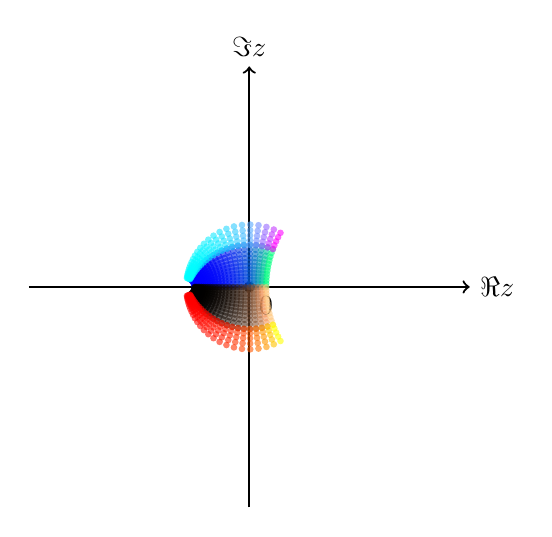
\begin{tikzpicture}[scale=0.8]

\draw[->, thick] (-3.5,0) -- (3.5,0) node[right] {$\Re z$};
\draw[->, thick] (0,-3.5) -- (0,3.5) node[above] {$\Im z$};

\fill (0,0) circle (2.5pt) node[below right] {$0$};

\fill[color={rgb,255:red,0; green,0; blue,255}, opacity=0.60] (-0.8505,0.0014) circle (1.5pt);
\fill[color={rgb,255:red,0; green,0; blue,255}, opacity=0.60] (-0.8310,0.0015) circle (1.5pt);
\fill[color={rgb,255:red,0; green,0; blue,255}, opacity=0.60] (-0.8092,0.0017) circle (1.5pt);
\fill[color={rgb,255:red,0; green,0; blue,255}, opacity=0.60] (-0.7849,0.0019) circle (1.5pt);
\fill[color={rgb,255:red,0; green,1; blue,254}, opacity=0.60] (-0.7580,0.0021) circle (1.5pt);
\fill[color={rgb,255:red,0; green,1; blue,254}, opacity=0.60] (-0.7282,0.0023) circle (1.5pt);
\fill[color={rgb,255:red,0; green,2; blue,254}, opacity=0.60] (-0.6953,0.0026) circle (1.5pt);
\fill[color={rgb,255:red,0; green,3; blue,253}, opacity=0.60] (-0.6593,0.0028) circle (1.5pt);
\fill[color={rgb,255:red,0; green,4; blue,253}, opacity=0.60] (-0.6199,0.0031) circle (1.5pt);
\fill[color={rgb,255:red,0; green,5; blue,252}, opacity=0.60] (-0.5772,0.0033) circle (1.5pt);
\fill[color={rgb,255:red,0; green,7; blue,251}, opacity=0.60] (-0.5311,0.0036) circle (1.5pt);
\fill[color={rgb,255:red,0; green,10; blue,250}, opacity=0.60] (-0.4815,0.0038) circle (1.5pt);
\fill[color={rgb,255:red,0; green,13; blue,248}, opacity=0.60] (-0.4287,0.0041) circle (1.5pt);
\fill[color={rgb,255:red,0; green,17; blue,246}, opacity=0.60] (-0.3728,0.0043) circle (1.5pt);
\fill[color={rgb,255:red,0; green,22; blue,244}, opacity=0.60] (-0.3141,0.0045) circle (1.5pt);
\fill[color={rgb,255:red,0; green,29; blue,240}, opacity=0.60] (-0.2528,0.0047) circle (1.5pt);
\fill[color={rgb,255:red,0; green,39; blue,235}, opacity=0.60] (-0.1895,0.0048) circle (1.5pt);
\fill[color={rgb,255:red,0; green,51; blue,229}, opacity=0.60] (-0.1245,0.0049) circle (1.5pt);
\fill[color={rgb,255:red,0; green,67; blue,221}, opacity=0.60] (-0.0585,0.0050) circle (1.5pt);
\fill[color={rgb,255:red,0; green,87; blue,211}, opacity=0.60] (0.0081,0.0050) circle (1.5pt);
\fill[color={rgb,255:red,0; green,113; blue,198}, opacity=0.60] (0.0746,0.0050) circle (1.5pt);
\fill[color={rgb,255:red,0; green,150; blue,179}, opacity=0.60] (0.1405,0.0049) circle (1.5pt);
\fill[color={rgb,255:red,0; green,195; blue,157}, opacity=0.60] (0.2051,0.0048) circle (1.5pt);
\fill[color={rgb,255:red,0; green,255; blue,127}, opacity=0.60] (0.2680,0.0046) circle (1.5pt);
\fill[color={rgb,255:red,0; green,0; blue,255}, opacity=0.60] (-0.8686,0.0143) circle (1.5pt);
\fill[color={rgb,255:red,0; green,0; blue,255}, opacity=0.60] (-0.8513,0.0161) circle (1.5pt);
\fill[color={rgb,255:red,0; green,0; blue,255}, opacity=0.60] (-0.8319,0.0180) circle (1.5pt);
\fill[color={rgb,255:red,0; green,0; blue,255}, opacity=0.60] (-0.8101,0.0200) circle (1.5pt);
\fill[color={rgb,255:red,0; green,0; blue,255}, opacity=0.60] (-0.7859,0.0223) circle (1.5pt);
\fill[color={rgb,255:red,0; green,1; blue,254}, opacity=0.60] (-0.7591,0.0247) circle (1.5pt);
\fill[color={rgb,255:red,0; green,1; blue,254}, opacity=0.60] (-0.7293,0.0273) circle (1.5pt);
\fill[color={rgb,255:red,0; green,2; blue,254}, opacity=0.60] (-0.6965,0.0300) circle (1.5pt);
\fill[color={rgb,255:red,0; green,3; blue,253}, opacity=0.60] (-0.6605,0.0328) circle (1.5pt);
\fill[color={rgb,255:red,0; green,4; blue,253}, opacity=0.60] (-0.6212,0.0358) circle (1.5pt);
\fill[color={rgb,255:red,0; green,5; blue,252}, opacity=0.60] (-0.5785,0.0387) circle (1.5pt);
\fill[color={rgb,255:red,0; green,7; blue,251}, opacity=0.60] (-0.5323,0.0417) circle (1.5pt);
\fill[color={rgb,255:red,0; green,10; blue,250}, opacity=0.60] (-0.4828,0.0446) circle (1.5pt);
\fill[color={rgb,255:red,0; green,13; blue,248}, opacity=0.60] (-0.4299,0.0474) circle (1.5pt);
\fill[color={rgb,255:red,0; green,17; blue,246}, opacity=0.60] (-0.3739,0.0501) circle (1.5pt);
\fill[color={rgb,255:red,0; green,22; blue,244}, opacity=0.60] (-0.3150,0.0524) circle (1.5pt);
\fill[color={rgb,255:red,0; green,29; blue,240}, opacity=0.60] (-0.2536,0.0544) circle (1.5pt);
\fill[color={rgb,255:red,0; green,39; blue,235}, opacity=0.60] (-0.1901,0.0561) circle (1.5pt);
\fill[color={rgb,255:red,0; green,51; blue,229}, opacity=0.60] (-0.1249,0.0573) circle (1.5pt);
\fill[color={rgb,255:red,0; green,67; blue,221}, opacity=0.60] (-0.0587,0.0580) circle (1.5pt);
\fill[color={rgb,255:red,0; green,87; blue,211}, opacity=0.60] (0.0081,0.0582) circle (1.5pt);
\fill[color={rgb,255:red,0; green,113; blue,198}, opacity=0.60] (0.0749,0.0578) circle (1.5pt);
\fill[color={rgb,255:red,0; green,150; blue,179}, opacity=0.60] (0.1409,0.0570) circle (1.5pt);
\fill[color={rgb,255:red,0; green,195; blue,157}, opacity=0.60] (0.2057,0.0557) circle (1.5pt);
\fill[color={rgb,255:red,0; green,255; blue,127}, opacity=0.60] (0.2688,0.0540) circle (1.5pt);
\fill[color={rgb,255:red,0; green,0; blue,255}, opacity=0.60] (-0.8706,0.0273) circle (1.5pt);
\fill[color={rgb,255:red,0; green,0; blue,255}, opacity=0.60] (-0.8534,0.0306) circle (1.5pt);
\fill[color={rgb,255:red,0; green,0; blue,255}, opacity=0.60] (-0.8342,0.0343) circle (1.5pt);
\fill[color={rgb,255:red,0; green,0; blue,255}, opacity=0.60] (-0.8126,0.0382) circle (1.5pt);
\fill[color={rgb,255:red,0; green,0; blue,255}, opacity=0.60] (-0.7886,0.0425) circle (1.5pt);
\fill[color={rgb,255:red,0; green,1; blue,254}, opacity=0.60] (-0.7620,0.0472) circle (1.5pt);
\fill[color={rgb,255:red,0; green,1; blue,254}, opacity=0.60] (-0.7324,0.0521) circle (1.5pt);
\fill[color={rgb,255:red,0; green,2; blue,254}, opacity=0.60] (-0.6997,0.0573) circle (1.5pt);
\fill[color={rgb,255:red,0; green,3; blue,253}, opacity=0.60] (-0.6639,0.0628) circle (1.5pt);
\fill[color={rgb,255:red,0; green,4; blue,253}, opacity=0.60] (-0.6247,0.0684) circle (1.5pt);
\fill[color={rgb,255:red,0; green,5; blue,252}, opacity=0.60] (-0.5820,0.0741) circle (1.5pt);
\fill[color={rgb,255:red,0; green,7; blue,251}, opacity=0.60] (-0.5358,0.0799) circle (1.5pt);
\fill[color={rgb,255:red,0; green,10; blue,250}, opacity=0.60] (-0.4861,0.0855) circle (1.5pt);
\fill[color={rgb,255:red,0; green,13; blue,248}, opacity=0.60] (-0.4331,0.0909) circle (1.5pt);
\fill[color={rgb,255:red,0; green,17; blue,246}, opacity=0.60] (-0.3768,0.0960) circle (1.5pt);
\fill[color={rgb,255:red,0; green,22; blue,244}, opacity=0.60] (-0.3176,0.1005) circle (1.5pt);
\fill[color={rgb,255:red,0; green,29; blue,240}, opacity=0.60] (-0.2558,0.1044) circle (1.5pt);
\fill[color={rgb,255:red,0; green,39; blue,235}, opacity=0.60] (-0.1917,0.1076) circle (1.5pt);
\fill[color={rgb,255:red,0; green,51; blue,229}, opacity=0.60] (-0.1260,0.1099) circle (1.5pt);
\fill[color={rgb,255:red,0; green,67; blue,221}, opacity=0.60] (-0.0592,0.1113) circle (1.5pt);
\fill[color={rgb,255:red,0; green,87; blue,211}, opacity=0.60] (0.0082,0.1116) circle (1.5pt);
\fill[color={rgb,255:red,0; green,113; blue,198}, opacity=0.60] (0.0755,0.1110) circle (1.5pt);
\fill[color={rgb,255:red,0; green,150; blue,179}, opacity=0.60] (0.1422,0.1094) circle (1.5pt);
\fill[color={rgb,255:red,0; green,195; blue,157}, opacity=0.60] (0.2075,0.1069) circle (1.5pt);
\fill[color={rgb,255:red,0; green,255; blue,127}, opacity=0.60] (0.2710,0.1035) circle (1.5pt);
\fill[color={rgb,255:red,0; green,0; blue,255}, opacity=0.60] (-0.8737,0.0401) circle (1.5pt);
\fill[color={rgb,255:red,0; green,0; blue,255}, opacity=0.60] (-0.8568,0.0450) circle (1.5pt);
\fill[color={rgb,255:red,0; green,0; blue,255}, opacity=0.60] (-0.8379,0.0503) circle (1.5pt);
\fill[color={rgb,255:red,0; green,0; blue,255}, opacity=0.60] (-0.8167,0.0562) circle (1.5pt);
\fill[color={rgb,255:red,0; green,0; blue,255}, opacity=0.60] (-0.7931,0.0626) circle (1.5pt);
\fill[color={rgb,255:red,0; green,1; blue,254}, opacity=0.60] (-0.7667,0.0694) circle (1.5pt);
\fill[color={rgb,255:red,0; green,1; blue,254}, opacity=0.60] (-0.7374,0.0768) circle (1.5pt);
\fill[color={rgb,255:red,0; green,2; blue,254}, opacity=0.60] (-0.7050,0.0845) circle (1.5pt);
\fill[color={rgb,255:red,0; green,3; blue,253}, opacity=0.60] (-0.6694,0.0926) circle (1.5pt);
\fill[color={rgb,255:red,0; green,4; blue,253}, opacity=0.60] (-0.6303,0.1010) circle (1.5pt);
\fill[color={rgb,255:red,0; green,5; blue,252}, opacity=0.60] (-0.5877,0.1095) circle (1.5pt);
\fill[color={rgb,255:red,0; green,7; blue,251}, opacity=0.60] (-0.5414,0.1181) circle (1.5pt);
\fill[color={rgb,255:red,0; green,10; blue,250}, opacity=0.60] (-0.4916,0.1265) circle (1.5pt);
\fill[color={rgb,255:red,0; green,13; blue,248}, opacity=0.60] (-0.4383,0.1346) circle (1.5pt);
\fill[color={rgb,255:red,0; green,17; blue,246}, opacity=0.60] (-0.3816,0.1422) circle (1.5pt);
\fill[color={rgb,255:red,0; green,22; blue,244}, opacity=0.60] (-0.3218,0.1490) circle (1.5pt);
\fill[color={rgb,255:red,0; green,29; blue,240}, opacity=0.60] (-0.2593,0.1549) circle (1.5pt);
\fill[color={rgb,255:red,0; green,39; blue,235}, opacity=0.60] (-0.1945,0.1597) circle (1.5pt);
\fill[color={rgb,255:red,0; green,51; blue,229}, opacity=0.60] (-0.1279,0.1631) circle (1.5pt);
\fill[color={rgb,255:red,0; green,67; blue,221}, opacity=0.60] (-0.0601,0.1652) circle (1.5pt);
\fill[color={rgb,255:red,0; green,87; blue,211}, opacity=0.60] (0.0083,0.1658) circle (1.5pt);
\fill[color={rgb,255:red,0; green,113; blue,198}, opacity=0.60] (0.0766,0.1648) circle (1.5pt);
\fill[color={rgb,255:red,0; green,150; blue,179}, opacity=0.60] (0.1442,0.1624) circle (1.5pt);
\fill[color={rgb,255:red,0; green,195; blue,157}, opacity=0.60] (0.2105,0.1586) circle (1.5pt);
\fill[color={rgb,255:red,0; green,255; blue,127}, opacity=0.60] (0.2748,0.1536) circle (1.5pt);
\fill[color={rgb,255:red,0; green,0; blue,255}, opacity=0.60] (-0.8780,0.0526) circle (1.5pt);
\fill[color={rgb,255:red,0; green,0; blue,255}, opacity=0.60] (-0.8616,0.0590) circle (1.5pt);
\fill[color={rgb,255:red,0; green,0; blue,255}, opacity=0.60] (-0.8431,0.0661) circle (1.5pt);
\fill[color={rgb,255:red,0; green,0; blue,255}, opacity=0.60] (-0.8224,0.0739) circle (1.5pt);
\fill[color={rgb,255:red,0; green,0; blue,255}, opacity=0.60] (-0.7992,0.0823) circle (1.5pt);
\fill[color={rgb,255:red,0; green,1; blue,254}, opacity=0.60] (-0.7733,0.0914) circle (1.5pt);
\fill[color={rgb,255:red,0; green,1; blue,254}, opacity=0.60] (-0.7444,0.1012) circle (1.5pt);
\fill[color={rgb,255:red,0; green,2; blue,254}, opacity=0.60] (-0.7124,0.1115) circle (1.5pt);
\fill[color={rgb,255:red,0; green,3; blue,253}, opacity=0.60] (-0.6771,0.1223) circle (1.5pt);
\fill[color={rgb,255:red,0; green,4; blue,253}, opacity=0.60] (-0.6382,0.1335) circle (1.5pt);
\fill[color={rgb,255:red,0; green,5; blue,252}, opacity=0.60] (-0.5957,0.1449) circle (1.5pt);
\fill[color={rgb,255:red,0; green,7; blue,251}, opacity=0.60] (-0.5494,0.1564) circle (1.5pt);
\fill[color={rgb,255:red,0; green,10; blue,250}, opacity=0.60] (-0.4994,0.1678) circle (1.5pt);
\fill[color={rgb,255:red,0; green,13; blue,248}, opacity=0.60] (-0.4456,0.1787) circle (1.5pt);
\fill[color={rgb,255:red,0; green,17; blue,246}, opacity=0.60] (-0.3884,0.1889) circle (1.5pt);
\fill[color={rgb,255:red,0; green,22; blue,244}, opacity=0.60] (-0.3278,0.1981) circle (1.5pt);
\fill[color={rgb,255:red,0; green,29; blue,240}, opacity=0.60] (-0.2643,0.2061) circle (1.5pt);
\fill[color={rgb,255:red,0; green,39; blue,235}, opacity=0.60] (-0.1984,0.2126) circle (1.5pt);
\fill[color={rgb,255:red,0; green,51; blue,229}, opacity=0.60] (-0.1305,0.2173) circle (1.5pt);
\fill[color={rgb,255:red,0; green,67; blue,221}, opacity=0.60] (-0.0613,0.2201) circle (1.5pt);
\fill[color={rgb,255:red,0; green,87; blue,211}, opacity=0.60] (0.0085,0.2209) circle (1.5pt);
\fill[color={rgb,255:red,0; green,113; blue,198}, opacity=0.60] (0.0782,0.2196) circle (1.5pt);
\fill[color={rgb,255:red,0; green,150; blue,179}, opacity=0.60] (0.1472,0.2163) circle (1.5pt);
\fill[color={rgb,255:red,0; green,195; blue,157}, opacity=0.60] (0.2146,0.2112) circle (1.5pt);
\fill[color={rgb,255:red,0; green,255; blue,127}, opacity=0.60] (0.2800,0.2043) circle (1.5pt);
\fill[color={rgb,255:red,0; green,0; blue,255}, opacity=0.60] (-0.8835,0.0647) circle (1.5pt);
\fill[color={rgb,255:red,0; green,0; blue,255}, opacity=0.60] (-0.8676,0.0727) circle (1.5pt);
\fill[color={rgb,255:red,0; green,0; blue,255}, opacity=0.60] (-0.8498,0.0815) circle (1.5pt);
\fill[color={rgb,255:red,0; green,0; blue,255}, opacity=0.60] (-0.8296,0.0911) circle (1.5pt);
\fill[color={rgb,255:red,0; green,0; blue,255}, opacity=0.60] (-0.8070,0.1016) circle (1.5pt);
\fill[color={rgb,255:red,0; green,1; blue,254}, opacity=0.60] (-0.7817,0.1130) circle (1.5pt);
\fill[color={rgb,255:red,0; green,1; blue,254}, opacity=0.60] (-0.7534,0.1252) circle (1.5pt);
\fill[color={rgb,255:red,0; green,2; blue,254}, opacity=0.60] (-0.7219,0.1381) circle (1.5pt);
\fill[color={rgb,255:red,0; green,3; blue,253}, opacity=0.60] (-0.6870,0.1517) circle (1.5pt);
\fill[color={rgb,255:red,0; green,4; blue,253}, opacity=0.60] (-0.6484,0.1658) circle (1.5pt);
\fill[color={rgb,255:red,0; green,5; blue,252}, opacity=0.60] (-0.6060,0.1803) circle (1.5pt);
\fill[color={rgb,255:red,0; green,7; blue,251}, opacity=0.60] (-0.5597,0.1949) circle (1.5pt);
\fill[color={rgb,255:red,0; green,10; blue,250}, opacity=0.60] (-0.5095,0.2093) circle (1.5pt);
\fill[color={rgb,255:red,0; green,13; blue,248}, opacity=0.60] (-0.4552,0.2232) circle (1.5pt);
\fill[color={rgb,255:red,0; green,17; blue,246}, opacity=0.60] (-0.3972,0.2362) circle (1.5pt);
\fill[color={rgb,255:red,0; green,22; blue,244}, opacity=0.60] (-0.3357,0.2480) circle (1.5pt);
\fill[color={rgb,255:red,0; green,29; blue,240}, opacity=0.60] (-0.2709,0.2583) circle (1.5pt);
\fill[color={rgb,255:red,0; green,39; blue,235}, opacity=0.60] (-0.2035,0.2666) circle (1.5pt);
\fill[color={rgb,255:red,0; green,51; blue,229}, opacity=0.60] (-0.1339,0.2726) circle (1.5pt);
\fill[color={rgb,255:red,0; green,67; blue,221}, opacity=0.60] (-0.0629,0.2763) circle (1.5pt);
\fill[color={rgb,255:red,0; green,87; blue,211}, opacity=0.60] (0.0087,0.2773) circle (1.5pt);
\fill[color={rgb,255:red,0; green,113; blue,198}, opacity=0.60] (0.0803,0.2756) circle (1.5pt);
\fill[color={rgb,255:red,0; green,150; blue,179}, opacity=0.60] (0.1510,0.2714) circle (1.5pt);
\fill[color={rgb,255:red,0; green,195; blue,157}, opacity=0.60] (0.2201,0.2648) circle (1.5pt);
\fill[color={rgb,255:red,0; green,255; blue,127}, opacity=0.60] (0.2870,0.2560) circle (1.5pt);
\fill[color={rgb,255:red,0; green,0; blue,255}, opacity=0.60] (-0.8901,0.0763) circle (1.5pt);
\fill[color={rgb,255:red,0; green,0; blue,255}, opacity=0.60] (-0.8750,0.0858) circle (1.5pt);
\fill[color={rgb,255:red,0; green,0; blue,255}, opacity=0.60] (-0.8578,0.0963) circle (1.5pt);
\fill[color={rgb,255:red,0; green,0; blue,255}, opacity=0.60] (-0.8385,0.1078) circle (1.5pt);
\fill[color={rgb,255:red,0; green,0; blue,255}, opacity=0.60] (-0.8166,0.1204) circle (1.5pt);
\fill[color={rgb,255:red,0; green,1; blue,254}, opacity=0.60] (-0.7920,0.1340) circle (1.5pt);
\fill[color={rgb,255:red,0; green,1; blue,254}, opacity=0.60] (-0.7645,0.1487) circle (1.5pt);
\fill[color={rgb,255:red,0; green,2; blue,254}, opacity=0.60] (-0.7336,0.1643) circle (1.5pt);
\fill[color={rgb,255:red,0; green,3; blue,253}, opacity=0.60] (-0.6992,0.1808) circle (1.5pt);
\fill[color={rgb,255:red,0; green,4; blue,253}, opacity=0.60] (-0.6611,0.1979) circle (1.5pt);
\fill[color={rgb,255:red,0; green,5; blue,252}, opacity=0.60] (-0.6189,0.2156) circle (1.5pt);
\fill[color={rgb,255:red,0; green,7; blue,251}, opacity=0.60] (-0.5726,0.2334) circle (1.5pt);
\fill[color={rgb,255:red,0; green,10; blue,250}, opacity=0.60] (-0.5221,0.2511) circle (1.5pt);
\fill[color={rgb,255:red,0; green,13; blue,248}, opacity=0.60] (-0.4673,0.2682) circle (1.5pt);
\fill[color={rgb,255:red,0; green,17; blue,246}, opacity=0.60] (-0.4084,0.2843) circle (1.5pt);
\fill[color={rgb,255:red,0; green,22; blue,244}, opacity=0.60] (-0.3456,0.2990) circle (1.5pt);
\fill[color={rgb,255:red,0; green,29; blue,240}, opacity=0.60] (-0.2792,0.3117) circle (1.5pt);
\fill[color={rgb,255:red,0; green,39; blue,235}, opacity=0.60] (-0.2099,0.3220) circle (1.5pt);
\fill[color={rgb,255:red,0; green,51; blue,229}, opacity=0.60] (-0.1383,0.3296) circle (1.5pt);
\fill[color={rgb,255:red,0; green,67; blue,221}, opacity=0.60] (-0.0650,0.3341) circle (1.5pt);
\fill[color={rgb,255:red,0; green,87; blue,211}, opacity=0.60] (0.0090,0.3353) circle (1.5pt);
\fill[color={rgb,255:red,0; green,113; blue,198}, opacity=0.60] (0.0829,0.3333) circle (1.5pt);
\fill[color={rgb,255:red,0; green,150; blue,179}, opacity=0.60] (0.1559,0.3280) circle (1.5pt);
\fill[color={rgb,255:red,0; green,195; blue,157}, opacity=0.60] (0.2271,0.3197) circle (1.5pt);
\fill[color={rgb,255:red,0; green,255; blue,127}, opacity=0.60] (0.2957,0.3088) circle (1.5pt);
\fill[color={rgb,255:red,0; green,0; blue,255}, opacity=0.60] (-0.8979,0.0873) circle (1.5pt);
\fill[color={rgb,255:red,0; green,0; blue,255}, opacity=0.60] (-0.8836,0.0983) circle (1.5pt);
\fill[color={rgb,255:red,0; green,0; blue,255}, opacity=0.60] (-0.8673,0.1105) circle (1.5pt);
\fill[color={rgb,255:red,0; green,0; blue,255}, opacity=0.60] (-0.8488,0.1239) circle (1.5pt);
\fill[color={rgb,255:red,0; green,0; blue,255}, opacity=0.60] (-0.8279,0.1385) circle (1.5pt);
\fill[color={rgb,255:red,0; green,1; blue,254}, opacity=0.60] (-0.8043,0.1544) circle (1.5pt);
\fill[color={rgb,255:red,0; green,1; blue,254}, opacity=0.60] (-0.7776,0.1716) circle (1.5pt);
\fill[color={rgb,255:red,0; green,2; blue,254}, opacity=0.60] (-0.7475,0.1900) circle (1.5pt);
\fill[color={rgb,255:red,0; green,3; blue,253}, opacity=0.60] (-0.7139,0.2094) circle (1.5pt);
\fill[color={rgb,255:red,0; green,4; blue,253}, opacity=0.60] (-0.6762,0.2297) circle (1.5pt);
\fill[color={rgb,255:red,0; green,5; blue,252}, opacity=0.60] (-0.6344,0.2507) circle (1.5pt);
\fill[color={rgb,255:red,0; green,7; blue,251}, opacity=0.60] (-0.5882,0.2720) circle (1.5pt);
\fill[color={rgb,255:red,0; green,10; blue,250}, opacity=0.60] (-0.5374,0.2932) circle (1.5pt);
\fill[color={rgb,255:red,0; green,13; blue,248}, opacity=0.60] (-0.4819,0.3138) circle (1.5pt);
\fill[color={rgb,255:red,0; green,17; blue,246}, opacity=0.60] (-0.4220,0.3333) circle (1.5pt);
\fill[color={rgb,255:red,0; green,22; blue,244}, opacity=0.60] (-0.3577,0.3511) circle (1.5pt);
\fill[color={rgb,255:red,0; green,29; blue,240}, opacity=0.60] (-0.2895,0.3666) circle (1.5pt);
\fill[color={rgb,255:red,0; green,39; blue,235}, opacity=0.60] (-0.2179,0.3792) circle (1.5pt);
\fill[color={rgb,255:red,0; green,51; blue,229}, opacity=0.60] (-0.1436,0.3885) circle (1.5pt);
\fill[color={rgb,255:red,0; green,67; blue,221}, opacity=0.60] (-0.0676,0.3940) circle (1.5pt);
\fill[color={rgb,255:red,0; green,87; blue,211}, opacity=0.60] (0.0094,0.3955) circle (1.5pt);
\fill[color={rgb,255:red,0; green,113; blue,198}, opacity=0.60] (0.0862,0.3930) circle (1.5pt);
\fill[color={rgb,255:red,0; green,150; blue,179}, opacity=0.60] (0.1619,0.3866) circle (1.5pt);
\fill[color={rgb,255:red,0; green,195; blue,157}, opacity=0.60] (0.2356,0.3764) circle (1.5pt);
\fill[color={rgb,255:red,0; green,255; blue,127}, opacity=0.60] (0.3064,0.3631) circle (1.5pt);
\fill[color={rgb,255:red,0; green,0; blue,255}, opacity=0.60] (-0.9068,0.0976) circle (1.5pt);
\fill[color={rgb,255:red,0; green,0; blue,255}, opacity=0.60] (-0.8934,0.1101) circle (1.5pt);
\fill[color={rgb,255:red,0; green,0; blue,255}, opacity=0.60] (-0.8782,0.1239) circle (1.5pt);
\fill[color={rgb,255:red,0; green,0; blue,255}, opacity=0.60] (-0.8608,0.1391) circle (1.5pt);
\fill[color={rgb,255:red,0; green,0; blue,255}, opacity=0.60] (-0.8410,0.1558) circle (1.5pt);
\fill[color={rgb,255:red,0; green,1; blue,254}, opacity=0.60] (-0.8184,0.1740) circle (1.5pt);
\fill[color={rgb,255:red,0; green,1; blue,254}, opacity=0.60] (-0.7928,0.1937) circle (1.5pt);
\fill[color={rgb,255:red,0; green,2; blue,254}, opacity=0.60] (-0.7638,0.2149) circle (1.5pt);
\fill[color={rgb,255:red,0; green,3; blue,253}, opacity=0.60] (-0.7310,0.2375) circle (1.5pt);
\fill[color={rgb,255:red,0; green,4; blue,253}, opacity=0.60] (-0.6941,0.2611) circle (1.5pt);
\fill[color={rgb,255:red,0; green,5; blue,252}, opacity=0.60] (-0.6528,0.2857) circle (1.5pt);
\fill[color={rgb,255:red,0; green,7; blue,251}, opacity=0.60] (-0.6067,0.3107) circle (1.5pt);
\fill[color={rgb,255:red,0; green,10; blue,250}, opacity=0.60] (-0.5556,0.3357) circle (1.5pt);
\fill[color={rgb,255:red,0; green,13; blue,248}, opacity=0.60] (-0.4995,0.3602) circle (1.5pt);
\fill[color={rgb,255:red,0; green,17; blue,246}, opacity=0.60] (-0.4383,0.3834) circle (1.5pt);
\fill[color={rgb,255:red,0; green,22; blue,244}, opacity=0.60] (-0.3723,0.4047) circle (1.5pt);
\fill[color={rgb,255:red,0; green,29; blue,240}, opacity=0.60] (-0.3019,0.4234) circle (1.5pt);
\fill[color={rgb,255:red,0; green,39; blue,235}, opacity=0.60] (-0.2276,0.4386) circle (1.5pt);
\fill[color={rgb,255:red,0; green,51; blue,229}, opacity=0.60] (-0.1502,0.4498) circle (1.5pt);
\fill[color={rgb,255:red,0; green,67; blue,221}, opacity=0.60] (-0.0707,0.4564) circle (1.5pt);
\fill[color={rgb,255:red,0; green,87; blue,211}, opacity=0.60] (0.0098,0.4583) circle (1.5pt);
\fill[color={rgb,255:red,0; green,113; blue,198}, opacity=0.60] (0.0902,0.4552) circle (1.5pt);
\fill[color={rgb,255:red,0; green,150; blue,179}, opacity=0.60] (0.1693,0.4474) circle (1.5pt);
\fill[color={rgb,255:red,0; green,195; blue,157}, opacity=0.60] (0.2460,0.4352) circle (1.5pt);
\fill[color={rgb,255:red,0; green,255; blue,127}, opacity=0.60] (0.3194,0.4191) circle (1.5pt);
\fill[color={rgb,255:red,0; green,0; blue,255}, opacity=0.60] (-0.9167,0.1072) circle (1.5pt);
\fill[color={rgb,255:red,0; green,0; blue,255}, opacity=0.60] (-0.9044,0.1210) circle (1.5pt);
\fill[color={rgb,255:red,0; green,0; blue,255}, opacity=0.60] (-0.8904,0.1364) circle (1.5pt);
\fill[color={rgb,255:red,0; green,0; blue,255}, opacity=0.60] (-0.8743,0.1534) circle (1.5pt);
\fill[color={rgb,255:red,0; green,0; blue,255}, opacity=0.60] (-0.8557,0.1721) circle (1.5pt);
\fill[color={rgb,255:red,0; green,1; blue,254}, opacity=0.60] (-0.8345,0.1926) circle (1.5pt);
\fill[color={rgb,255:red,0; green,1; blue,254}, opacity=0.60] (-0.8102,0.2150) circle (1.5pt);
\fill[color={rgb,255:red,0; green,2; blue,254}, opacity=0.60] (-0.7824,0.2390) circle (1.5pt);
\fill[color={rgb,255:red,0; green,3; blue,253}, opacity=0.60] (-0.7508,0.2648) circle (1.5pt);
\fill[color={rgb,255:red,0; green,4; blue,253}, opacity=0.60] (-0.7148,0.2919) circle (1.5pt);
\fill[color={rgb,255:red,0; green,5; blue,252}, opacity=0.60] (-0.6741,0.3203) circle (1.5pt);
\fill[color={rgb,255:red,0; green,7; blue,251}, opacity=0.60] (-0.6283,0.3493) circle (1.5pt);
\fill[color={rgb,255:red,0; green,10; blue,250}, opacity=0.60] (-0.5771,0.3786) circle (1.5pt);
\fill[color={rgb,255:red,0; green,13; blue,248}, opacity=0.60] (-0.5203,0.4073) circle (1.5pt);
\fill[color={rgb,255:red,0; green,17; blue,246}, opacity=0.60] (-0.4578,0.4348) circle (1.5pt);
\fill[color={rgb,255:red,0; green,22; blue,244}, opacity=0.60] (-0.3898,0.4601) circle (1.5pt);
\fill[color={rgb,255:red,0; green,29; blue,240}, opacity=0.60] (-0.3167,0.4823) circle (1.5pt);
\fill[color={rgb,255:red,0; green,39; blue,235}, opacity=0.60] (-0.2392,0.5005) circle (1.5pt);
\fill[color={rgb,255:red,0; green,51; blue,229}, opacity=0.60] (-0.1581,0.5139) circle (1.5pt);
\fill[color={rgb,255:red,0; green,67; blue,221}, opacity=0.60] (-0.0744,0.5220) circle (1.5pt);
\fill[color={rgb,255:red,0; green,87; blue,211}, opacity=0.60] (0.0103,0.5242) circle (1.5pt);
\fill[color={rgb,255:red,0; green,113; blue,198}, opacity=0.60] (0.0950,0.5205) circle (1.5pt);
\fill[color={rgb,255:red,0; green,150; blue,179}, opacity=0.60] (0.1781,0.5111) circle (1.5pt);
\fill[color={rgb,255:red,0; green,195; blue,157}, opacity=0.60] (0.2584,0.4965) circle (1.5pt);
\fill[color={rgb,255:red,0; green,255; blue,127}, opacity=0.60] (0.3350,0.4772) circle (1.5pt);
\fill[color={rgb,255:red,0; green,0; blue,255}, opacity=0.60] (-0.9276,0.1158) circle (1.5pt);
\fill[color={rgb,255:red,0; green,0; blue,255}, opacity=0.60] (-0.9166,0.1309) circle (1.5pt);
\fill[color={rgb,255:red,0; green,0; blue,255}, opacity=0.60] (-0.9039,0.1478) circle (1.5pt);
\fill[color={rgb,255:red,0; green,0; blue,255}, opacity=0.60] (-0.8892,0.1666) circle (1.5pt);
\fill[color={rgb,255:red,0; green,0; blue,255}, opacity=0.60] (-0.8722,0.1873) circle (1.5pt);
\fill[color={rgb,255:red,0; green,1; blue,254}, opacity=0.60] (-0.8526,0.2101) circle (1.5pt);
\fill[color={rgb,255:red,0; green,1; blue,254}, opacity=0.60] (-0.8298,0.2351) circle (1.5pt);
\fill[color={rgb,255:red,0; green,2; blue,254}, opacity=0.60] (-0.8035,0.2621) circle (1.5pt);
\fill[color={rgb,255:red,0; green,3; blue,253}, opacity=0.60] (-0.7733,0.2912) circle (1.5pt);
\fill[color={rgb,255:red,0; green,4; blue,253}, opacity=0.60] (-0.7385,0.3220) circle (1.5pt);
\fill[color={rgb,255:red,0; green,5; blue,252}, opacity=0.60] (-0.6987,0.3544) circle (1.5pt);
\fill[color={rgb,255:red,0; green,7; blue,251}, opacity=0.60] (-0.6534,0.3879) circle (1.5pt);
\fill[color={rgb,255:red,0; green,10; blue,250}, opacity=0.60] (-0.6021,0.4217) circle (1.5pt);
\fill[color={rgb,255:red,0; green,13; blue,248}, opacity=0.60] (-0.5446,0.4553) circle (1.5pt);
\fill[color={rgb,255:red,0; green,17; blue,246}, opacity=0.60] (-0.4808,0.4875) circle (1.5pt);
\fill[color={rgb,255:red,0; green,22; blue,244}, opacity=0.60] (-0.4106,0.5174) circle (1.5pt);
\fill[color={rgb,255:red,0; green,29; blue,240}, opacity=0.60] (-0.3345,0.5437) circle (1.5pt);
\fill[color={rgb,255:red,0; green,39; blue,235}, opacity=0.60] (-0.2531,0.5655) circle (1.5pt);
\fill[color={rgb,255:red,0; green,51; blue,229}, opacity=0.60] (-0.1675,0.5816) circle (1.5pt);
\fill[color={rgb,255:red,0; green,67; blue,221}, opacity=0.60] (-0.0790,0.5912) circle (1.5pt);
\fill[color={rgb,255:red,0; green,87; blue,211}, opacity=0.60] (0.0110,0.5939) circle (1.5pt);
\fill[color={rgb,255:red,0; green,113; blue,198}, opacity=0.60] (0.1007,0.5895) circle (1.5pt);
\fill[color={rgb,255:red,0; green,150; blue,179}, opacity=0.60] (0.1887,0.5782) circle (1.5pt);
\fill[color={rgb,255:red,0; green,195; blue,157}, opacity=0.60] (0.2734,0.5606) circle (1.5pt);
\fill[color={rgb,255:red,0; green,255; blue,127}, opacity=0.60] (0.3535,0.5377) circle (1.5pt);
\fill[color={rgb,255:red,0; green,0; blue,255}, opacity=0.60] (-0.9395,0.1234) circle (1.5pt);
\fill[color={rgb,255:red,0; green,0; blue,255}, opacity=0.60] (-0.9299,0.1397) circle (1.5pt);
\fill[color={rgb,255:red,0; green,0; blue,255}, opacity=0.60] (-0.9187,0.1581) circle (1.5pt);
\fill[color={rgb,255:red,0; green,0; blue,255}, opacity=0.60] (-0.9057,0.1785) circle (1.5pt);
\fill[color={rgb,255:red,0; green,0; blue,255}, opacity=0.60] (-0.8904,0.2012) circle (1.5pt);
\fill[color={rgb,255:red,0; green,1; blue,254}, opacity=0.60] (-0.8726,0.2263) circle (1.5pt);
\fill[color={rgb,255:red,0; green,1; blue,254}, opacity=0.60] (-0.8516,0.2538) circle (1.5pt);
\fill[color={rgb,255:red,0; green,2; blue,254}, opacity=0.60] (-0.8272,0.2839) circle (1.5pt);
\fill[color={rgb,255:red,0; green,3; blue,253}, opacity=0.60] (-0.7986,0.3164) circle (1.5pt);
\fill[color={rgb,255:red,0; green,4; blue,253}, opacity=0.60] (-0.7654,0.3512) circle (1.5pt);
\fill[color={rgb,255:red,0; green,5; blue,252}, opacity=0.60] (-0.7268,0.3879) circle (1.5pt);
\fill[color={rgb,255:red,0; green,7; blue,251}, opacity=0.60] (-0.6822,0.4261) circle (1.5pt);
\fill[color={rgb,255:red,0; green,10; blue,250}, opacity=0.60] (-0.6312,0.4651) circle (1.5pt);
\fill[color={rgb,255:red,0; green,13; blue,248}, opacity=0.60] (-0.5731,0.5040) circle (1.5pt);
\fill[color={rgb,255:red,0; green,17; blue,246}, opacity=0.60] (-0.5078,0.5417) circle (1.5pt);
\fill[color={rgb,255:red,0; green,22; blue,244}, opacity=0.60] (-0.4351,0.5769) circle (1.5pt);
\fill[color={rgb,255:red,0; green,29; blue,240}, opacity=0.60] (-0.3555,0.6081) circle (1.5pt);
\fill[color={rgb,255:red,0; green,39; blue,235}, opacity=0.60] (-0.2697,0.6340) circle (1.5pt);
\fill[color={rgb,255:red,0; green,51; blue,229}, opacity=0.60] (-0.1789,0.6533) circle (1.5pt);
\fill[color={rgb,255:red,0; green,67; blue,221}, opacity=0.60] (-0.0844,0.6649) circle (1.5pt);
\fill[color={rgb,255:red,0; green,87; blue,211}, opacity=0.60] (0.0117,0.6681) circle (1.5pt);
\fill[color={rgb,255:red,0; green,113; blue,198}, opacity=0.60] (0.1077,0.6628) circle (1.5pt);
\fill[color={rgb,255:red,0; green,150; blue,179}, opacity=0.60] (0.2014,0.6493) circle (1.5pt);
\fill[color={rgb,255:red,0; green,195; blue,157}, opacity=0.60] (0.2912,0.6283) circle (1.5pt);
\fill[color={rgb,255:red,0; green,255; blue,127}, opacity=0.60] (0.3755,0.6009) circle (1.5pt);
\fill[color={rgb,255:red,0; green,0; blue,0}, opacity=0.60] (-0.9395,-0.1234) circle (1.5pt);
\fill[color={rgb,255:red,0; green,0; blue,0}, opacity=0.60] (-0.9299,-0.1397) circle (1.5pt);
\fill[color={rgb,255:red,0; green,0; blue,0}, opacity=0.60] (-0.9187,-0.1581) circle (1.5pt);
\fill[color={rgb,255:red,0; green,0; blue,0}, opacity=0.60] (-0.9057,-0.1785) circle (1.5pt);
\fill[color={rgb,255:red,0; green,0; blue,0}, opacity=0.60] (-0.8904,-0.2012) circle (1.5pt);
\fill[color={rgb,255:red,1; green,0; blue,0}, opacity=0.60] (-0.8726,-0.2263) circle (1.5pt);
\fill[color={rgb,255:red,1; green,0; blue,0}, opacity=0.60] (-0.8516,-0.2538) circle (1.5pt);
\fill[color={rgb,255:red,2; green,1; blue,0}, opacity=0.60] (-0.8272,-0.2839) circle (1.5pt);
\fill[color={rgb,255:red,3; green,2; blue,1}, opacity=0.60] (-0.7986,-0.3164) circle (1.5pt);
\fill[color={rgb,255:red,4; green,3; blue,1}, opacity=0.60] (-0.7654,-0.3512) circle (1.5pt);
\fill[color={rgb,255:red,6; green,3; blue,2}, opacity=0.60] (-0.7268,-0.3879) circle (1.5pt);
\fill[color={rgb,255:red,8; green,5; blue,3}, opacity=0.60] (-0.6822,-0.4261) circle (1.5pt);
\fill[color={rgb,255:red,12; green,7; blue,4}, opacity=0.60] (-0.6312,-0.4651) circle (1.5pt);
\fill[color={rgb,255:red,16; green,10; blue,6}, opacity=0.60] (-0.5731,-0.5040) circle (1.5pt);
\fill[color={rgb,255:red,20; green,13; blue,8}, opacity=0.60] (-0.5078,-0.5417) circle (1.5pt);
\fill[color={rgb,255:red,27; green,17; blue,10}, opacity=0.60] (-0.4351,-0.5769) circle (1.5pt);
\fill[color={rgb,255:red,35; green,22; blue,14}, opacity=0.60] (-0.3555,-0.6081) circle (1.5pt);
\fill[color={rgb,255:red,48; green,30; blue,19}, opacity=0.60] (-0.2697,-0.6340) circle (1.5pt);
\fill[color={rgb,255:red,62; green,39; blue,25}, opacity=0.60] (-0.1789,-0.6533) circle (1.5pt);
\fill[color={rgb,255:red,82; green,52; blue,33}, opacity=0.60] (-0.0844,-0.6649) circle (1.5pt);
\fill[color={rgb,255:red,107; green,67; blue,43}, opacity=0.60] (0.0117,-0.6681) circle (1.5pt);
\fill[color={rgb,255:red,140; green,89; blue,56}, opacity=0.60] (0.1077,-0.6628) circle (1.5pt);
\fill[color={rgb,255:red,185; green,117; blue,74}, opacity=0.60] (0.2014,-0.6493) circle (1.5pt);
\fill[color={rgb,255:red,242; green,153; blue,97}, opacity=0.60] (0.2912,-0.6283) circle (1.5pt);
\fill[color={rgb,255:red,255; green,199; blue,126}, opacity=0.60] (0.3755,-0.6009) circle (1.5pt);
\fill[color={rgb,255:red,0; green,0; blue,0}, opacity=0.60] (-0.9276,-0.1158) circle (1.5pt);
\fill[color={rgb,255:red,0; green,0; blue,0}, opacity=0.60] (-0.9166,-0.1309) circle (1.5pt);
\fill[color={rgb,255:red,0; green,0; blue,0}, opacity=0.60] (-0.9039,-0.1478) circle (1.5pt);
\fill[color={rgb,255:red,0; green,0; blue,0}, opacity=0.60] (-0.8892,-0.1666) circle (1.5pt);
\fill[color={rgb,255:red,0; green,0; blue,0}, opacity=0.60] (-0.8722,-0.1873) circle (1.5pt);
\fill[color={rgb,255:red,1; green,0; blue,0}, opacity=0.60] (-0.8526,-0.2101) circle (1.5pt);
\fill[color={rgb,255:red,1; green,0; blue,0}, opacity=0.60] (-0.8298,-0.2351) circle (1.5pt);
\fill[color={rgb,255:red,2; green,1; blue,0}, opacity=0.60] (-0.8035,-0.2621) circle (1.5pt);
\fill[color={rgb,255:red,3; green,2; blue,1}, opacity=0.60] (-0.7733,-0.2912) circle (1.5pt);
\fill[color={rgb,255:red,4; green,3; blue,1}, opacity=0.60] (-0.7385,-0.3220) circle (1.5pt);
\fill[color={rgb,255:red,6; green,3; blue,2}, opacity=0.60] (-0.6987,-0.3544) circle (1.5pt);
\fill[color={rgb,255:red,8; green,5; blue,3}, opacity=0.60] (-0.6534,-0.3879) circle (1.5pt);
\fill[color={rgb,255:red,12; green,7; blue,4}, opacity=0.60] (-0.6021,-0.4217) circle (1.5pt);
\fill[color={rgb,255:red,16; green,10; blue,6}, opacity=0.60] (-0.5446,-0.4553) circle (1.5pt);
\fill[color={rgb,255:red,20; green,13; blue,8}, opacity=0.60] (-0.4808,-0.4875) circle (1.5pt);
\fill[color={rgb,255:red,27; green,17; blue,10}, opacity=0.60] (-0.4106,-0.5174) circle (1.5pt);
\fill[color={rgb,255:red,35; green,22; blue,14}, opacity=0.60] (-0.3345,-0.5437) circle (1.5pt);
\fill[color={rgb,255:red,48; green,30; blue,19}, opacity=0.60] (-0.2531,-0.5655) circle (1.5pt);
\fill[color={rgb,255:red,62; green,39; blue,25}, opacity=0.60] (-0.1675,-0.5816) circle (1.5pt);
\fill[color={rgb,255:red,82; green,52; blue,33}, opacity=0.60] (-0.0790,-0.5912) circle (1.5pt);
\fill[color={rgb,255:red,107; green,67; blue,43}, opacity=0.60] (0.0110,-0.5939) circle (1.5pt);
\fill[color={rgb,255:red,140; green,89; blue,56}, opacity=0.60] (0.1007,-0.5895) circle (1.5pt);
\fill[color={rgb,255:red,185; green,117; blue,74}, opacity=0.60] (0.1887,-0.5782) circle (1.5pt);
\fill[color={rgb,255:red,242; green,153; blue,97}, opacity=0.60] (0.2734,-0.5606) circle (1.5pt);
\fill[color={rgb,255:red,255; green,199; blue,126}, opacity=0.60] (0.3535,-0.5377) circle (1.5pt);
\fill[color={rgb,255:red,0; green,0; blue,0}, opacity=0.60] (-0.9167,-0.1072) circle (1.5pt);
\fill[color={rgb,255:red,0; green,0; blue,0}, opacity=0.60] (-0.9044,-0.1210) circle (1.5pt);
\fill[color={rgb,255:red,0; green,0; blue,0}, opacity=0.60] (-0.8904,-0.1364) circle (1.5pt);
\fill[color={rgb,255:red,0; green,0; blue,0}, opacity=0.60] (-0.8743,-0.1534) circle (1.5pt);
\fill[color={rgb,255:red,0; green,0; blue,0}, opacity=0.60] (-0.8557,-0.1721) circle (1.5pt);
\fill[color={rgb,255:red,1; green,0; blue,0}, opacity=0.60] (-0.8345,-0.1926) circle (1.5pt);
\fill[color={rgb,255:red,1; green,0; blue,0}, opacity=0.60] (-0.8102,-0.2150) circle (1.5pt);
\fill[color={rgb,255:red,2; green,1; blue,0}, opacity=0.60] (-0.7824,-0.2390) circle (1.5pt);
\fill[color={rgb,255:red,3; green,2; blue,1}, opacity=0.60] (-0.7508,-0.2648) circle (1.5pt);
\fill[color={rgb,255:red,4; green,3; blue,1}, opacity=0.60] (-0.7148,-0.2919) circle (1.5pt);
\fill[color={rgb,255:red,6; green,3; blue,2}, opacity=0.60] (-0.6741,-0.3203) circle (1.5pt);
\fill[color={rgb,255:red,8; green,5; blue,3}, opacity=0.60] (-0.6283,-0.3493) circle (1.5pt);
\fill[color={rgb,255:red,12; green,7; blue,4}, opacity=0.60] (-0.5771,-0.3786) circle (1.5pt);
\fill[color={rgb,255:red,16; green,10; blue,6}, opacity=0.60] (-0.5203,-0.4073) circle (1.5pt);
\fill[color={rgb,255:red,20; green,13; blue,8}, opacity=0.60] (-0.4578,-0.4348) circle (1.5pt);
\fill[color={rgb,255:red,27; green,17; blue,10}, opacity=0.60] (-0.3898,-0.4601) circle (1.5pt);
\fill[color={rgb,255:red,35; green,22; blue,14}, opacity=0.60] (-0.3167,-0.4823) circle (1.5pt);
\fill[color={rgb,255:red,48; green,30; blue,19}, opacity=0.60] (-0.2392,-0.5005) circle (1.5pt);
\fill[color={rgb,255:red,62; green,39; blue,25}, opacity=0.60] (-0.1581,-0.5139) circle (1.5pt);
\fill[color={rgb,255:red,82; green,52; blue,33}, opacity=0.60] (-0.0744,-0.5220) circle (1.5pt);
\fill[color={rgb,255:red,107; green,67; blue,43}, opacity=0.60] (0.0103,-0.5242) circle (1.5pt);
\fill[color={rgb,255:red,140; green,89; blue,56}, opacity=0.60] (0.0950,-0.5205) circle (1.5pt);
\fill[color={rgb,255:red,185; green,117; blue,74}, opacity=0.60] (0.1781,-0.5111) circle (1.5pt);
\fill[color={rgb,255:red,242; green,153; blue,97}, opacity=0.60] (0.2584,-0.4965) circle (1.5pt);
\fill[color={rgb,255:red,255; green,199; blue,126}, opacity=0.60] (0.3350,-0.4772) circle (1.5pt);
\fill[color={rgb,255:red,0; green,0; blue,0}, opacity=0.60] (-0.9068,-0.0976) circle (1.5pt);
\fill[color={rgb,255:red,0; green,0; blue,0}, opacity=0.60] (-0.8934,-0.1101) circle (1.5pt);
\fill[color={rgb,255:red,0; green,0; blue,0}, opacity=0.60] (-0.8782,-0.1239) circle (1.5pt);
\fill[color={rgb,255:red,0; green,0; blue,0}, opacity=0.60] (-0.8608,-0.1391) circle (1.5pt);
\fill[color={rgb,255:red,0; green,0; blue,0}, opacity=0.60] (-0.8410,-0.1558) circle (1.5pt);
\fill[color={rgb,255:red,1; green,0; blue,0}, opacity=0.60] (-0.8184,-0.1740) circle (1.5pt);
\fill[color={rgb,255:red,1; green,0; blue,0}, opacity=0.60] (-0.7928,-0.1937) circle (1.5pt);
\fill[color={rgb,255:red,2; green,1; blue,0}, opacity=0.60] (-0.7638,-0.2149) circle (1.5pt);
\fill[color={rgb,255:red,3; green,2; blue,1}, opacity=0.60] (-0.7310,-0.2375) circle (1.5pt);
\fill[color={rgb,255:red,4; green,3; blue,1}, opacity=0.60] (-0.6941,-0.2611) circle (1.5pt);
\fill[color={rgb,255:red,6; green,3; blue,2}, opacity=0.60] (-0.6528,-0.2857) circle (1.5pt);
\fill[color={rgb,255:red,8; green,5; blue,3}, opacity=0.60] (-0.6067,-0.3107) circle (1.5pt);
\fill[color={rgb,255:red,12; green,7; blue,4}, opacity=0.60] (-0.5556,-0.3357) circle (1.5pt);
\fill[color={rgb,255:red,16; green,10; blue,6}, opacity=0.60] (-0.4995,-0.3602) circle (1.5pt);
\fill[color={rgb,255:red,20; green,13; blue,8}, opacity=0.60] (-0.4383,-0.3834) circle (1.5pt);
\fill[color={rgb,255:red,27; green,17; blue,10}, opacity=0.60] (-0.3723,-0.4047) circle (1.5pt);
\fill[color={rgb,255:red,35; green,22; blue,14}, opacity=0.60] (-0.3019,-0.4234) circle (1.5pt);
\fill[color={rgb,255:red,48; green,30; blue,19}, opacity=0.60] (-0.2276,-0.4386) circle (1.5pt);
\fill[color={rgb,255:red,62; green,39; blue,25}, opacity=0.60] (-0.1502,-0.4498) circle (1.5pt);
\fill[color={rgb,255:red,82; green,52; blue,33}, opacity=0.60] (-0.0707,-0.4564) circle (1.5pt);
\fill[color={rgb,255:red,107; green,67; blue,43}, opacity=0.60] (0.0098,-0.4583) circle (1.5pt);
\fill[color={rgb,255:red,140; green,89; blue,56}, opacity=0.60] (0.0902,-0.4552) circle (1.5pt);
\fill[color={rgb,255:red,185; green,117; blue,74}, opacity=0.60] (0.1693,-0.4474) circle (1.5pt);
\fill[color={rgb,255:red,242; green,153; blue,97}, opacity=0.60] (0.2460,-0.4352) circle (1.5pt);
\fill[color={rgb,255:red,255; green,199; blue,126}, opacity=0.60] (0.3194,-0.4191) circle (1.5pt);
\fill[color={rgb,255:red,0; green,0; blue,0}, opacity=0.60] (-0.8979,-0.0873) circle (1.5pt);
\fill[color={rgb,255:red,0; green,0; blue,0}, opacity=0.60] (-0.8836,-0.0983) circle (1.5pt);
\fill[color={rgb,255:red,0; green,0; blue,0}, opacity=0.60] (-0.8673,-0.1105) circle (1.5pt);
\fill[color={rgb,255:red,0; green,0; blue,0}, opacity=0.60] (-0.8488,-0.1239) circle (1.5pt);
\fill[color={rgb,255:red,0; green,0; blue,0}, opacity=0.60] (-0.8279,-0.1385) circle (1.5pt);
\fill[color={rgb,255:red,1; green,0; blue,0}, opacity=0.60] (-0.8043,-0.1544) circle (1.5pt);
\fill[color={rgb,255:red,1; green,0; blue,0}, opacity=0.60] (-0.7776,-0.1716) circle (1.5pt);
\fill[color={rgb,255:red,2; green,1; blue,0}, opacity=0.60] (-0.7475,-0.1900) circle (1.5pt);
\fill[color={rgb,255:red,3; green,2; blue,1}, opacity=0.60] (-0.7139,-0.2094) circle (1.5pt);
\fill[color={rgb,255:red,4; green,3; blue,1}, opacity=0.60] (-0.6762,-0.2297) circle (1.5pt);
\fill[color={rgb,255:red,6; green,3; blue,2}, opacity=0.60] (-0.6344,-0.2507) circle (1.5pt);
\fill[color={rgb,255:red,8; green,5; blue,3}, opacity=0.60] (-0.5882,-0.2720) circle (1.5pt);
\fill[color={rgb,255:red,12; green,7; blue,4}, opacity=0.60] (-0.5374,-0.2932) circle (1.5pt);
\fill[color={rgb,255:red,16; green,10; blue,6}, opacity=0.60] (-0.4819,-0.3138) circle (1.5pt);
\fill[color={rgb,255:red,20; green,13; blue,8}, opacity=0.60] (-0.4220,-0.3333) circle (1.5pt);
\fill[color={rgb,255:red,27; green,17; blue,10}, opacity=0.60] (-0.3577,-0.3511) circle (1.5pt);
\fill[color={rgb,255:red,35; green,22; blue,14}, opacity=0.60] (-0.2895,-0.3666) circle (1.5pt);
\fill[color={rgb,255:red,48; green,30; blue,19}, opacity=0.60] (-0.2179,-0.3792) circle (1.5pt);
\fill[color={rgb,255:red,62; green,39; blue,25}, opacity=0.60] (-0.1436,-0.3885) circle (1.5pt);
\fill[color={rgb,255:red,82; green,52; blue,33}, opacity=0.60] (-0.0676,-0.3940) circle (1.5pt);
\fill[color={rgb,255:red,107; green,67; blue,43}, opacity=0.60] (0.0094,-0.3955) circle (1.5pt);
\fill[color={rgb,255:red,140; green,89; blue,56}, opacity=0.60] (0.0862,-0.3930) circle (1.5pt);
\fill[color={rgb,255:red,185; green,117; blue,74}, opacity=0.60] (0.1619,-0.3866) circle (1.5pt);
\fill[color={rgb,255:red,242; green,153; blue,97}, opacity=0.60] (0.2356,-0.3764) circle (1.5pt);
\fill[color={rgb,255:red,255; green,199; blue,126}, opacity=0.60] (0.3064,-0.3631) circle (1.5pt);
\fill[color={rgb,255:red,0; green,0; blue,0}, opacity=0.60] (-0.8901,-0.0763) circle (1.5pt);
\fill[color={rgb,255:red,0; green,0; blue,0}, opacity=0.60] (-0.8750,-0.0858) circle (1.5pt);
\fill[color={rgb,255:red,0; green,0; blue,0}, opacity=0.60] (-0.8578,-0.0963) circle (1.5pt);
\fill[color={rgb,255:red,0; green,0; blue,0}, opacity=0.60] (-0.8385,-0.1078) circle (1.5pt);
\fill[color={rgb,255:red,0; green,0; blue,0}, opacity=0.60] (-0.8166,-0.1204) circle (1.5pt);
\fill[color={rgb,255:red,1; green,0; blue,0}, opacity=0.60] (-0.7920,-0.1340) circle (1.5pt);
\fill[color={rgb,255:red,1; green,0; blue,0}, opacity=0.60] (-0.7645,-0.1487) circle (1.5pt);
\fill[color={rgb,255:red,2; green,1; blue,0}, opacity=0.60] (-0.7336,-0.1643) circle (1.5pt);
\fill[color={rgb,255:red,3; green,2; blue,1}, opacity=0.60] (-0.6992,-0.1808) circle (1.5pt);
\fill[color={rgb,255:red,4; green,3; blue,1}, opacity=0.60] (-0.6611,-0.1979) circle (1.5pt);
\fill[color={rgb,255:red,6; green,3; blue,2}, opacity=0.60] (-0.6189,-0.2156) circle (1.5pt);
\fill[color={rgb,255:red,8; green,5; blue,3}, opacity=0.60] (-0.5726,-0.2334) circle (1.5pt);
\fill[color={rgb,255:red,12; green,7; blue,4}, opacity=0.60] (-0.5221,-0.2511) circle (1.5pt);
\fill[color={rgb,255:red,16; green,10; blue,6}, opacity=0.60] (-0.4673,-0.2682) circle (1.5pt);
\fill[color={rgb,255:red,20; green,13; blue,8}, opacity=0.60] (-0.4084,-0.2843) circle (1.5pt);
\fill[color={rgb,255:red,27; green,17; blue,10}, opacity=0.60] (-0.3456,-0.2990) circle (1.5pt);
\fill[color={rgb,255:red,35; green,22; blue,14}, opacity=0.60] (-0.2792,-0.3117) circle (1.5pt);
\fill[color={rgb,255:red,48; green,30; blue,19}, opacity=0.60] (-0.2099,-0.3220) circle (1.5pt);
\fill[color={rgb,255:red,62; green,39; blue,25}, opacity=0.60] (-0.1383,-0.3296) circle (1.5pt);
\fill[color={rgb,255:red,82; green,52; blue,33}, opacity=0.60] (-0.0650,-0.3341) circle (1.5pt);
\fill[color={rgb,255:red,107; green,67; blue,43}, opacity=0.60] (0.0090,-0.3353) circle (1.5pt);
\fill[color={rgb,255:red,140; green,89; blue,56}, opacity=0.60] (0.0829,-0.3333) circle (1.5pt);
\fill[color={rgb,255:red,185; green,117; blue,74}, opacity=0.60] (0.1559,-0.3280) circle (1.5pt);
\fill[color={rgb,255:red,242; green,153; blue,97}, opacity=0.60] (0.2271,-0.3197) circle (1.5pt);
\fill[color={rgb,255:red,255; green,199; blue,126}, opacity=0.60] (0.2957,-0.3088) circle (1.5pt);
\fill[color={rgb,255:red,0; green,0; blue,0}, opacity=0.60] (-0.8835,-0.0647) circle (1.5pt);
\fill[color={rgb,255:red,0; green,0; blue,0}, opacity=0.60] (-0.8676,-0.0727) circle (1.5pt);
\fill[color={rgb,255:red,0; green,0; blue,0}, opacity=0.60] (-0.8498,-0.0815) circle (1.5pt);
\fill[color={rgb,255:red,0; green,0; blue,0}, opacity=0.60] (-0.8296,-0.0911) circle (1.5pt);
\fill[color={rgb,255:red,0; green,0; blue,0}, opacity=0.60] (-0.8070,-0.1016) circle (1.5pt);
\fill[color={rgb,255:red,1; green,0; blue,0}, opacity=0.60] (-0.7817,-0.1130) circle (1.5pt);
\fill[color={rgb,255:red,1; green,0; blue,0}, opacity=0.60] (-0.7534,-0.1252) circle (1.5pt);
\fill[color={rgb,255:red,2; green,1; blue,0}, opacity=0.60] (-0.7219,-0.1381) circle (1.5pt);
\fill[color={rgb,255:red,3; green,2; blue,1}, opacity=0.60] (-0.6870,-0.1517) circle (1.5pt);
\fill[color={rgb,255:red,4; green,3; blue,1}, opacity=0.60] (-0.6484,-0.1658) circle (1.5pt);
\fill[color={rgb,255:red,6; green,3; blue,2}, opacity=0.60] (-0.6060,-0.1803) circle (1.5pt);
\fill[color={rgb,255:red,8; green,5; blue,3}, opacity=0.60] (-0.5597,-0.1949) circle (1.5pt);
\fill[color={rgb,255:red,12; green,7; blue,4}, opacity=0.60] (-0.5095,-0.2093) circle (1.5pt);
\fill[color={rgb,255:red,16; green,10; blue,6}, opacity=0.60] (-0.4552,-0.2232) circle (1.5pt);
\fill[color={rgb,255:red,20; green,13; blue,8}, opacity=0.60] (-0.3972,-0.2362) circle (1.5pt);
\fill[color={rgb,255:red,27; green,17; blue,10}, opacity=0.60] (-0.3357,-0.2480) circle (1.5pt);
\fill[color={rgb,255:red,35; green,22; blue,14}, opacity=0.60] (-0.2709,-0.2583) circle (1.5pt);
\fill[color={rgb,255:red,48; green,30; blue,19}, opacity=0.60] (-0.2035,-0.2666) circle (1.5pt);
\fill[color={rgb,255:red,62; green,39; blue,25}, opacity=0.60] (-0.1339,-0.2726) circle (1.5pt);
\fill[color={rgb,255:red,82; green,52; blue,33}, opacity=0.60] (-0.0629,-0.2763) circle (1.5pt);
\fill[color={rgb,255:red,107; green,67; blue,43}, opacity=0.60] (0.0087,-0.2773) circle (1.5pt);
\fill[color={rgb,255:red,140; green,89; blue,56}, opacity=0.60] (0.0803,-0.2756) circle (1.5pt);
\fill[color={rgb,255:red,185; green,117; blue,74}, opacity=0.60] (0.1510,-0.2714) circle (1.5pt);
\fill[color={rgb,255:red,242; green,153; blue,97}, opacity=0.60] (0.2201,-0.2648) circle (1.5pt);
\fill[color={rgb,255:red,255; green,199; blue,126}, opacity=0.60] (0.2870,-0.2560) circle (1.5pt);
\fill[color={rgb,255:red,0; green,0; blue,0}, opacity=0.60] (-0.8780,-0.0526) circle (1.5pt);
\fill[color={rgb,255:red,0; green,0; blue,0}, opacity=0.60] (-0.8616,-0.0590) circle (1.5pt);
\fill[color={rgb,255:red,0; green,0; blue,0}, opacity=0.60] (-0.8431,-0.0661) circle (1.5pt);
\fill[color={rgb,255:red,0; green,0; blue,0}, opacity=0.60] (-0.8224,-0.0739) circle (1.5pt);
\fill[color={rgb,255:red,0; green,0; blue,0}, opacity=0.60] (-0.7992,-0.0823) circle (1.5pt);
\fill[color={rgb,255:red,1; green,0; blue,0}, opacity=0.60] (-0.7733,-0.0914) circle (1.5pt);
\fill[color={rgb,255:red,1; green,0; blue,0}, opacity=0.60] (-0.7444,-0.1012) circle (1.5pt);
\fill[color={rgb,255:red,2; green,1; blue,0}, opacity=0.60] (-0.7124,-0.1115) circle (1.5pt);
\fill[color={rgb,255:red,3; green,2; blue,1}, opacity=0.60] (-0.6771,-0.1223) circle (1.5pt);
\fill[color={rgb,255:red,4; green,3; blue,1}, opacity=0.60] (-0.6382,-0.1335) circle (1.5pt);
\fill[color={rgb,255:red,6; green,3; blue,2}, opacity=0.60] (-0.5957,-0.1449) circle (1.5pt);
\fill[color={rgb,255:red,8; green,5; blue,3}, opacity=0.60] (-0.5494,-0.1564) circle (1.5pt);
\fill[color={rgb,255:red,12; green,7; blue,4}, opacity=0.60] (-0.4994,-0.1678) circle (1.5pt);
\fill[color={rgb,255:red,16; green,10; blue,6}, opacity=0.60] (-0.4456,-0.1787) circle (1.5pt);
\fill[color={rgb,255:red,20; green,13; blue,8}, opacity=0.60] (-0.3884,-0.1889) circle (1.5pt);
\fill[color={rgb,255:red,27; green,17; blue,10}, opacity=0.60] (-0.3278,-0.1981) circle (1.5pt);
\fill[color={rgb,255:red,35; green,22; blue,14}, opacity=0.60] (-0.2643,-0.2061) circle (1.5pt);
\fill[color={rgb,255:red,48; green,30; blue,19}, opacity=0.60] (-0.1984,-0.2126) circle (1.5pt);
\fill[color={rgb,255:red,62; green,39; blue,25}, opacity=0.60] (-0.1305,-0.2173) circle (1.5pt);
\fill[color={rgb,255:red,82; green,52; blue,33}, opacity=0.60] (-0.0613,-0.2201) circle (1.5pt);
\fill[color={rgb,255:red,107; green,67; blue,43}, opacity=0.60] (0.0085,-0.2209) circle (1.5pt);
\fill[color={rgb,255:red,140; green,89; blue,56}, opacity=0.60] (0.0782,-0.2196) circle (1.5pt);
\fill[color={rgb,255:red,185; green,117; blue,74}, opacity=0.60] (0.1472,-0.2163) circle (1.5pt);
\fill[color={rgb,255:red,242; green,153; blue,97}, opacity=0.60] (0.2146,-0.2112) circle (1.5pt);
\fill[color={rgb,255:red,255; green,199; blue,126}, opacity=0.60] (0.2800,-0.2043) circle (1.5pt);
\fill[color={rgb,255:red,0; green,0; blue,0}, opacity=0.60] (-0.8737,-0.0401) circle (1.5pt);
\fill[color={rgb,255:red,0; green,0; blue,0}, opacity=0.60] (-0.8568,-0.0450) circle (1.5pt);
\fill[color={rgb,255:red,0; green,0; blue,0}, opacity=0.60] (-0.8379,-0.0503) circle (1.5pt);
\fill[color={rgb,255:red,0; green,0; blue,0}, opacity=0.60] (-0.8167,-0.0562) circle (1.5pt);
\fill[color={rgb,255:red,0; green,0; blue,0}, opacity=0.60] (-0.7931,-0.0626) circle (1.5pt);
\fill[color={rgb,255:red,1; green,0; blue,0}, opacity=0.60] (-0.7667,-0.0694) circle (1.5pt);
\fill[color={rgb,255:red,1; green,0; blue,0}, opacity=0.60] (-0.7374,-0.0768) circle (1.5pt);
\fill[color={rgb,255:red,2; green,1; blue,0}, opacity=0.60] (-0.7050,-0.0845) circle (1.5pt);
\fill[color={rgb,255:red,3; green,2; blue,1}, opacity=0.60] (-0.6694,-0.0926) circle (1.5pt);
\fill[color={rgb,255:red,4; green,3; blue,1}, opacity=0.60] (-0.6303,-0.1010) circle (1.5pt);
\fill[color={rgb,255:red,6; green,3; blue,2}, opacity=0.60] (-0.5877,-0.1095) circle (1.5pt);
\fill[color={rgb,255:red,8; green,5; blue,3}, opacity=0.60] (-0.5414,-0.1181) circle (1.5pt);
\fill[color={rgb,255:red,12; green,7; blue,4}, opacity=0.60] (-0.4916,-0.1265) circle (1.5pt);
\fill[color={rgb,255:red,16; green,10; blue,6}, opacity=0.60] (-0.4383,-0.1346) circle (1.5pt);
\fill[color={rgb,255:red,20; green,13; blue,8}, opacity=0.60] (-0.3816,-0.1422) circle (1.5pt);
\fill[color={rgb,255:red,27; green,17; blue,10}, opacity=0.60] (-0.3218,-0.1490) circle (1.5pt);
\fill[color={rgb,255:red,35; green,22; blue,14}, opacity=0.60] (-0.2593,-0.1549) circle (1.5pt);
\fill[color={rgb,255:red,48; green,30; blue,19}, opacity=0.60] (-0.1945,-0.1597) circle (1.5pt);
\fill[color={rgb,255:red,62; green,39; blue,25}, opacity=0.60] (-0.1279,-0.1631) circle (1.5pt);
\fill[color={rgb,255:red,82; green,52; blue,33}, opacity=0.60] (-0.0601,-0.1652) circle (1.5pt);
\fill[color={rgb,255:red,107; green,67; blue,43}, opacity=0.60] (0.0083,-0.1658) circle (1.5pt);
\fill[color={rgb,255:red,140; green,89; blue,56}, opacity=0.60] (0.0766,-0.1648) circle (1.5pt);
\fill[color={rgb,255:red,185; green,117; blue,74}, opacity=0.60] (0.1442,-0.1624) circle (1.5pt);
\fill[color={rgb,255:red,242; green,153; blue,97}, opacity=0.60] (0.2105,-0.1586) circle (1.5pt);
\fill[color={rgb,255:red,255; green,199; blue,126}, opacity=0.60] (0.2748,-0.1536) circle (1.5pt);
\fill[color={rgb,255:red,0; green,0; blue,0}, opacity=0.60] (-0.8706,-0.0273) circle (1.5pt);
\fill[color={rgb,255:red,0; green,0; blue,0}, opacity=0.60] (-0.8534,-0.0306) circle (1.5pt);
\fill[color={rgb,255:red,0; green,0; blue,0}, opacity=0.60] (-0.8342,-0.0343) circle (1.5pt);
\fill[color={rgb,255:red,0; green,0; blue,0}, opacity=0.60] (-0.8126,-0.0382) circle (1.5pt);
\fill[color={rgb,255:red,0; green,0; blue,0}, opacity=0.60] (-0.7886,-0.0425) circle (1.5pt);
\fill[color={rgb,255:red,1; green,0; blue,0}, opacity=0.60] (-0.7620,-0.0472) circle (1.5pt);
\fill[color={rgb,255:red,1; green,0; blue,0}, opacity=0.60] (-0.7324,-0.0521) circle (1.5pt);
\fill[color={rgb,255:red,2; green,1; blue,0}, opacity=0.60] (-0.6997,-0.0573) circle (1.5pt);
\fill[color={rgb,255:red,3; green,2; blue,1}, opacity=0.60] (-0.6639,-0.0628) circle (1.5pt);
\fill[color={rgb,255:red,4; green,3; blue,1}, opacity=0.60] (-0.6247,-0.0684) circle (1.5pt);
\fill[color={rgb,255:red,6; green,3; blue,2}, opacity=0.60] (-0.5820,-0.0741) circle (1.5pt);
\fill[color={rgb,255:red,8; green,5; blue,3}, opacity=0.60] (-0.5358,-0.0799) circle (1.5pt);
\fill[color={rgb,255:red,12; green,7; blue,4}, opacity=0.60] (-0.4861,-0.0855) circle (1.5pt);
\fill[color={rgb,255:red,16; green,10; blue,6}, opacity=0.60] (-0.4331,-0.0909) circle (1.5pt);
\fill[color={rgb,255:red,20; green,13; blue,8}, opacity=0.60] (-0.3768,-0.0960) circle (1.5pt);
\fill[color={rgb,255:red,27; green,17; blue,10}, opacity=0.60] (-0.3176,-0.1005) circle (1.5pt);
\fill[color={rgb,255:red,35; green,22; blue,14}, opacity=0.60] (-0.2558,-0.1044) circle (1.5pt);
\fill[color={rgb,255:red,48; green,30; blue,19}, opacity=0.60] (-0.1917,-0.1076) circle (1.5pt);
\fill[color={rgb,255:red,62; green,39; blue,25}, opacity=0.60] (-0.1260,-0.1099) circle (1.5pt);
\fill[color={rgb,255:red,82; green,52; blue,33}, opacity=0.60] (-0.0592,-0.1113) circle (1.5pt);
\fill[color={rgb,255:red,107; green,67; blue,43}, opacity=0.60] (0.0082,-0.1116) circle (1.5pt);
\fill[color={rgb,255:red,140; green,89; blue,56}, opacity=0.60] (0.0755,-0.1110) circle (1.5pt);
\fill[color={rgb,255:red,185; green,117; blue,74}, opacity=0.60] (0.1422,-0.1094) circle (1.5pt);
\fill[color={rgb,255:red,242; green,153; blue,97}, opacity=0.60] (0.2075,-0.1069) circle (1.5pt);
\fill[color={rgb,255:red,255; green,199; blue,126}, opacity=0.60] (0.2710,-0.1035) circle (1.5pt);
\fill[color={rgb,255:red,0; green,0; blue,0}, opacity=0.60] (-0.8686,-0.0143) circle (1.5pt);
\fill[color={rgb,255:red,0; green,0; blue,0}, opacity=0.60] (-0.8513,-0.0161) circle (1.5pt);
\fill[color={rgb,255:red,0; green,0; blue,0}, opacity=0.60] (-0.8319,-0.0180) circle (1.5pt);
\fill[color={rgb,255:red,0; green,0; blue,0}, opacity=0.60] (-0.8101,-0.0200) circle (1.5pt);
\fill[color={rgb,255:red,0; green,0; blue,0}, opacity=0.60] (-0.7859,-0.0223) circle (1.5pt);
\fill[color={rgb,255:red,1; green,0; blue,0}, opacity=0.60] (-0.7591,-0.0247) circle (1.5pt);
\fill[color={rgb,255:red,1; green,0; blue,0}, opacity=0.60] (-0.7293,-0.0273) circle (1.5pt);
\fill[color={rgb,255:red,2; green,1; blue,0}, opacity=0.60] (-0.6965,-0.0300) circle (1.5pt);
\fill[color={rgb,255:red,3; green,2; blue,1}, opacity=0.60] (-0.6605,-0.0328) circle (1.5pt);
\fill[color={rgb,255:red,4; green,3; blue,1}, opacity=0.60] (-0.6212,-0.0358) circle (1.5pt);
\fill[color={rgb,255:red,6; green,3; blue,2}, opacity=0.60] (-0.5785,-0.0387) circle (1.5pt);
\fill[color={rgb,255:red,8; green,5; blue,3}, opacity=0.60] (-0.5323,-0.0417) circle (1.5pt);
\fill[color={rgb,255:red,12; green,7; blue,4}, opacity=0.60] (-0.4828,-0.0446) circle (1.5pt);
\fill[color={rgb,255:red,16; green,10; blue,6}, opacity=0.60] (-0.4299,-0.0474) circle (1.5pt);
\fill[color={rgb,255:red,20; green,13; blue,8}, opacity=0.60] (-0.3739,-0.0501) circle (1.5pt);
\fill[color={rgb,255:red,27; green,17; blue,10}, opacity=0.60] (-0.3150,-0.0524) circle (1.5pt);
\fill[color={rgb,255:red,35; green,22; blue,14}, opacity=0.60] (-0.2536,-0.0544) circle (1.5pt);
\fill[color={rgb,255:red,48; green,30; blue,19}, opacity=0.60] (-0.1901,-0.0561) circle (1.5pt);
\fill[color={rgb,255:red,62; green,39; blue,25}, opacity=0.60] (-0.1249,-0.0573) circle (1.5pt);
\fill[color={rgb,255:red,82; green,52; blue,33}, opacity=0.60] (-0.0587,-0.0580) circle (1.5pt);
\fill[color={rgb,255:red,107; green,67; blue,43}, opacity=0.60] (0.0081,-0.0582) circle (1.5pt);
\fill[color={rgb,255:red,140; green,89; blue,56}, opacity=0.60] (0.0749,-0.0578) circle (1.5pt);
\fill[color={rgb,255:red,185; green,117; blue,74}, opacity=0.60] (0.1409,-0.0570) circle (1.5pt);
\fill[color={rgb,255:red,242; green,153; blue,97}, opacity=0.60] (0.2057,-0.0557) circle (1.5pt);
\fill[color={rgb,255:red,255; green,199; blue,126}, opacity=0.60] (0.2688,-0.0540) circle (1.5pt);
\fill[color={rgb,255:red,0; green,0; blue,0}, opacity=0.60] (-0.8679,-0.0012) circle (1.5pt);
\fill[color={rgb,255:red,0; green,0; blue,0}, opacity=0.60] (-0.8505,-0.0014) circle (1.5pt);
\fill[color={rgb,255:red,0; green,0; blue,0}, opacity=0.60] (-0.8310,-0.0015) circle (1.5pt);
\fill[color={rgb,255:red,0; green,0; blue,0}, opacity=0.60] (-0.8092,-0.0017) circle (1.5pt);
\fill[color={rgb,255:red,0; green,0; blue,0}, opacity=0.60] (-0.7849,-0.0019) circle (1.5pt);
\fill[color={rgb,255:red,1; green,0; blue,0}, opacity=0.60] (-0.7580,-0.0021) circle (1.5pt);
\fill[color={rgb,255:red,1; green,0; blue,0}, opacity=0.60] (-0.7282,-0.0023) circle (1.5pt);
\fill[color={rgb,255:red,2; green,1; blue,0}, opacity=0.60] (-0.6953,-0.0026) circle (1.5pt);
\fill[color={rgb,255:red,3; green,2; blue,1}, opacity=0.60] (-0.6593,-0.0028) circle (1.5pt);
\fill[color={rgb,255:red,4; green,3; blue,1}, opacity=0.60] (-0.6199,-0.0031) circle (1.5pt);
\fill[color={rgb,255:red,6; green,3; blue,2}, opacity=0.60] (-0.5772,-0.0033) circle (1.5pt);
\fill[color={rgb,255:red,8; green,5; blue,3}, opacity=0.60] (-0.5311,-0.0036) circle (1.5pt);
\fill[color={rgb,255:red,12; green,7; blue,4}, opacity=0.60] (-0.4815,-0.0038) circle (1.5pt);
\fill[color={rgb,255:red,16; green,10; blue,6}, opacity=0.60] (-0.4287,-0.0041) circle (1.5pt);
\fill[color={rgb,255:red,20; green,13; blue,8}, opacity=0.60] (-0.3728,-0.0043) circle (1.5pt);
\fill[color={rgb,255:red,27; green,17; blue,10}, opacity=0.60] (-0.3141,-0.0045) circle (1.5pt);
\fill[color={rgb,255:red,35; green,22; blue,14}, opacity=0.60] (-0.2528,-0.0047) circle (1.5pt);
\fill[color={rgb,255:red,48; green,30; blue,19}, opacity=0.60] (-0.1895,-0.0048) circle (1.5pt);
\fill[color={rgb,255:red,62; green,39; blue,25}, opacity=0.60] (-0.1245,-0.0049) circle (1.5pt);
\fill[color={rgb,255:red,82; green,52; blue,33}, opacity=0.60] (-0.0585,-0.0050) circle (1.5pt);
\fill[color={rgb,255:red,107; green,67; blue,43}, opacity=0.60] (0.0081,-0.0050) circle (1.5pt);
\fill[color={rgb,255:red,140; green,89; blue,56}, opacity=0.60] (0.0746,-0.0050) circle (1.5pt);
\fill[color={rgb,255:red,185; green,117; blue,74}, opacity=0.60] (0.1405,-0.0049) circle (1.5pt);
\fill[color={rgb,255:red,242; green,153; blue,97}, opacity=0.60] (0.2051,-0.0048) circle (1.5pt);
\fill[color={rgb,255:red,255; green,199; blue,126}, opacity=0.60] (0.2680,-0.0046) circle (1.5pt);
\fill[color={rgb,255:red,0; green,255; blue,255}, opacity=0.60] (-0.9395,0.1234) circle (1.5pt);
\fill[color={rgb,255:red,0; green,255; blue,255}, opacity=0.60] (-0.9299,0.1397) circle (1.5pt);
\fill[color={rgb,255:red,0; green,255; blue,255}, opacity=0.60] (-0.9187,0.1581) circle (1.5pt);
\fill[color={rgb,255:red,0; green,255; blue,255}, opacity=0.60] (-0.9057,0.1785) circle (1.5pt);
\fill[color={rgb,255:red,0; green,255; blue,255}, opacity=0.60] (-0.8904,0.2012) circle (1.5pt);
\fill[color={rgb,255:red,1; green,254; blue,255}, opacity=0.60] (-0.8726,0.2263) circle (1.5pt);
\fill[color={rgb,255:red,1; green,254; blue,255}, opacity=0.60] (-0.8516,0.2538) circle (1.5pt);
\fill[color={rgb,255:red,2; green,253; blue,255}, opacity=0.60] (-0.8272,0.2839) circle (1.5pt);
\fill[color={rgb,255:red,3; green,252; blue,255}, opacity=0.60] (-0.7986,0.3164) circle (1.5pt);
\fill[color={rgb,255:red,4; green,251; blue,255}, opacity=0.60] (-0.7654,0.3512) circle (1.5pt);
\fill[color={rgb,255:red,5; green,250; blue,255}, opacity=0.60] (-0.7268,0.3879) circle (1.5pt);
\fill[color={rgb,255:red,7; green,248; blue,255}, opacity=0.60] (-0.6822,0.4261) circle (1.5pt);
\fill[color={rgb,255:red,10; green,245; blue,255}, opacity=0.60] (-0.6312,0.4651) circle (1.5pt);
\fill[color={rgb,255:red,13; green,242; blue,255}, opacity=0.60] (-0.5731,0.5040) circle (1.5pt);
\fill[color={rgb,255:red,17; green,238; blue,255}, opacity=0.60] (-0.5078,0.5417) circle (1.5pt);
\fill[color={rgb,255:red,22; green,233; blue,255}, opacity=0.60] (-0.4351,0.5769) circle (1.5pt);
\fill[color={rgb,255:red,29; green,226; blue,255}, opacity=0.60] (-0.3555,0.6081) circle (1.5pt);
\fill[color={rgb,255:red,39; green,216; blue,255}, opacity=0.60] (-0.2697,0.6340) circle (1.5pt);
\fill[color={rgb,255:red,51; green,204; blue,255}, opacity=0.60] (-0.1789,0.6533) circle (1.5pt);
\fill[color={rgb,255:red,67; green,188; blue,255}, opacity=0.60] (-0.0844,0.6649) circle (1.5pt);
\fill[color={rgb,255:red,87; green,168; blue,255}, opacity=0.60] (0.0117,0.6681) circle (1.5pt);
\fill[color={rgb,255:red,113; green,141; blue,255}, opacity=0.60] (0.1077,0.6628) circle (1.5pt);
\fill[color={rgb,255:red,150; green,105; blue,255}, opacity=0.60] (0.2014,0.6493) circle (1.5pt);
\fill[color={rgb,255:red,195; green,59; blue,255}, opacity=0.60] (0.2912,0.6283) circle (1.5pt);
\fill[color={rgb,255:red,255; green,0; blue,255}, opacity=0.60] (0.3755,0.6009) circle (1.5pt);
\fill[color={rgb,255:red,0; green,255; blue,255}, opacity=0.60] (-0.9509,0.1292) circle (1.5pt);
\fill[color={rgb,255:red,0; green,255; blue,255}, opacity=0.60] (-0.9427,0.1466) circle (1.5pt);
\fill[color={rgb,255:red,0; green,255; blue,255}, opacity=0.60] (-0.9331,0.1661) circle (1.5pt);
\fill[color={rgb,255:red,0; green,255; blue,255}, opacity=0.60] (-0.9217,0.1880) circle (1.5pt);
\fill[color={rgb,255:red,0; green,255; blue,255}, opacity=0.60] (-0.9082,0.2124) circle (1.5pt);
\fill[color={rgb,255:red,1; green,254; blue,255}, opacity=0.60] (-0.8922,0.2395) circle (1.5pt);
\fill[color={rgb,255:red,1; green,254; blue,255}, opacity=0.60] (-0.8732,0.2694) circle (1.5pt);
\fill[color={rgb,255:red,2; green,253; blue,255}, opacity=0.60] (-0.8507,0.3022) circle (1.5pt);
\fill[color={rgb,255:red,3; green,252; blue,255}, opacity=0.60] (-0.8240,0.3379) circle (1.5pt);
\fill[color={rgb,255:red,4; green,251; blue,255}, opacity=0.60] (-0.7925,0.3763) circle (1.5pt);
\fill[color={rgb,255:red,5; green,250; blue,255}, opacity=0.60] (-0.7553,0.4172) circle (1.5pt);
\fill[color={rgb,255:red,7; green,248; blue,255}, opacity=0.60] (-0.7118,0.4601) circle (1.5pt);
\fill[color={rgb,255:red,10; green,245; blue,255}, opacity=0.60] (-0.6611,0.5042) circle (1.5pt);
\fill[color={rgb,255:red,13; green,242; blue,255}, opacity=0.60] (-0.6027,0.5486) circle (1.5pt);
\fill[color={rgb,255:red,17; green,238; blue,255}, opacity=0.60] (-0.5360,0.5919) circle (1.5pt);
\fill[color={rgb,255:red,22; green,233; blue,255}, opacity=0.60] (-0.4610,0.6326) circle (1.5pt);
\fill[color={rgb,255:red,29; green,226; blue,255}, opacity=0.60] (-0.3779,0.6690) circle (1.5pt);
\fill[color={rgb,255:red,39; green,216; blue,255}, opacity=0.60] (-0.2875,0.6994) circle (1.5pt);
\fill[color={rgb,255:red,51; green,204; blue,255}, opacity=0.60] (-0.1910,0.7221) circle (1.5pt);
\fill[color={rgb,255:red,67; green,188; blue,255}, opacity=0.60] (-0.0903,0.7358) circle (1.5pt);
\fill[color={rgb,255:red,87; green,168; blue,255}, opacity=0.60] (0.0126,0.7396) circle (1.5pt);
\fill[color={rgb,255:red,113; green,141; blue,255}, opacity=0.60] (0.1151,0.7334) circle (1.5pt);
\fill[color={rgb,255:red,150; green,105; blue,255}, opacity=0.60] (0.2150,0.7174) circle (1.5pt);
\fill[color={rgb,255:red,195; green,59; blue,255}, opacity=0.60] (0.3101,0.6927) circle (1.5pt);
\fill[color={rgb,255:red,255; green,0; blue,255}, opacity=0.60] (0.3989,0.6607) circle (1.5pt);
\fill[color={rgb,255:red,0; green,255; blue,255}, opacity=0.60] (-0.9629,0.1341) circle (1.5pt);
\fill[color={rgb,255:red,0; green,255; blue,255}, opacity=0.60] (-0.9563,0.1524) circle (1.5pt);
\fill[color={rgb,255:red,0; green,255; blue,255}, opacity=0.60] (-0.9484,0.1730) circle (1.5pt);
\fill[color={rgb,255:red,0; green,255; blue,255}, opacity=0.60] (-0.9388,0.1962) circle (1.5pt);
\fill[color={rgb,255:red,0; green,255; blue,255}, opacity=0.60] (-0.9273,0.2222) circle (1.5pt);
\fill[color={rgb,255:red,1; green,254; blue,255}, opacity=0.60] (-0.9134,0.2512) circle (1.5pt);
\fill[color={rgb,255:red,1; green,254; blue,255}, opacity=0.60] (-0.8966,0.2834) circle (1.5pt);
\fill[color={rgb,255:red,2; green,253; blue,255}, opacity=0.60] (-0.8764,0.3190) circle (1.5pt);
\fill[color={rgb,255:red,3; green,252; blue,255}, opacity=0.60] (-0.8519,0.3579) circle (1.5pt);
\fill[color={rgb,255:red,4; green,251; blue,255}, opacity=0.60] (-0.8225,0.4002) circle (1.5pt);
\fill[color={rgb,255:red,5; green,250; blue,255}, opacity=0.60] (-0.7872,0.4455) circle (1.5pt);
\fill[color={rgb,255:red,7; green,248; blue,255}, opacity=0.60] (-0.7450,0.4935) circle (1.5pt);
\fill[color={rgb,255:red,10; green,245; blue,255}, opacity=0.60] (-0.6951,0.5432) circle (1.5pt);
\fill[color={rgb,255:red,13; green,242; blue,255}, opacity=0.60] (-0.6365,0.5937) circle (1.5pt);
\fill[color={rgb,255:red,17; green,238; blue,255}, opacity=0.60] (-0.5687,0.6434) circle (1.5pt);
\fill[color={rgb,255:red,22; green,233; blue,255}, opacity=0.60] (-0.4912,0.6905) circle (1.5pt);
\fill[color={rgb,255:red,29; green,226; blue,255}, opacity=0.60] (-0.4042,0.7331) circle (1.5pt);
\fill[color={rgb,255:red,39; green,216; blue,255}, opacity=0.60] (-0.3084,0.7688) circle (1.5pt);
\fill[color={rgb,255:red,51; green,204; blue,255}, opacity=0.60] (-0.2054,0.7956) circle (1.5pt);
\fill[color={rgb,255:red,67; green,188; blue,255}, opacity=0.60] (-0.0972,0.8119) circle (1.5pt);
\fill[color={rgb,255:red,87; green,168; blue,255}, opacity=0.60] (0.0135,0.8164) circle (1.5pt);
\fill[color={rgb,255:red,113; green,141; blue,255}, opacity=0.60] (0.1239,0.8090) circle (1.5pt);
\fill[color={rgb,255:red,150; green,105; blue,255}, opacity=0.60] (0.2310,0.7900) circle (1.5pt);
\fill[color={rgb,255:red,195; green,59; blue,255}, opacity=0.60] (0.3325,0.7608) circle (1.5pt);
\fill[color={rgb,255:red,255; green,0; blue,255}, opacity=0.60] (0.4262,0.7233) circle (1.5pt);
\fill[color={rgb,255:red,0; green,255; blue,255}, opacity=0.60] (-0.9756,0.1379) circle (1.5pt);
\fill[color={rgb,255:red,0; green,255; blue,255}, opacity=0.60] (-0.9706,0.1570) circle (1.5pt);
\fill[color={rgb,255:red,0; green,255; blue,255}, opacity=0.60] (-0.9645,0.1786) circle (1.5pt);
\fill[color={rgb,255:red,0; green,255; blue,255}, opacity=0.60] (-0.9569,0.2030) circle (1.5pt);
\fill[color={rgb,255:red,0; green,255; blue,255}, opacity=0.60] (-0.9476,0.2305) circle (1.5pt);
\fill[color={rgb,255:red,1; green,254; blue,255}, opacity=0.60] (-0.9361,0.2613) circle (1.5pt);
\fill[color={rgb,255:red,1; green,254; blue,255}, opacity=0.60] (-0.9218,0.2957) circle (1.5pt);
\fill[color={rgb,255:red,2; green,253; blue,255}, opacity=0.60] (-0.9042,0.3340) circle (1.5pt);
\fill[color={rgb,255:red,3; green,252; blue,255}, opacity=0.60] (-0.8824,0.3763) circle (1.5pt);
\fill[color={rgb,255:red,4; green,251; blue,255}, opacity=0.60] (-0.8555,0.4225) circle (1.5pt);
\fill[color={rgb,255:red,5; green,250; blue,255}, opacity=0.60] (-0.8225,0.4725) circle (1.5pt);
\fill[color={rgb,255:red,7; green,248; blue,255}, opacity=0.60] (-0.7822,0.5259) circle (1.5pt);
\fill[color={rgb,255:red,10; green,245; blue,255}, opacity=0.60] (-0.7335,0.5818) circle (1.5pt);
\fill[color={rgb,255:red,13; green,242; blue,255}, opacity=0.60] (-0.6752,0.6391) circle (1.5pt);
\fill[color={rgb,255:red,17; green,238; blue,255}, opacity=0.60] (-0.6063,0.6962) circle (1.5pt);
\fill[color={rgb,255:red,22; green,233; blue,255}, opacity=0.60] (-0.5262,0.7509) circle (1.5pt);
\fill[color={rgb,255:red,29; green,226; blue,255}, opacity=0.60] (-0.4349,0.8006) circle (1.5pt);
\fill[color={rgb,255:red,39; green,216; blue,255}, opacity=0.60] (-0.3331,0.8428) circle (1.5pt);
\fill[color={rgb,255:red,51; green,204; blue,255}, opacity=0.60] (-0.2225,0.8746) circle (1.5pt);
\fill[color={rgb,255:red,67; green,188; blue,255}, opacity=0.60] (-0.1055,0.8940) circle (1.5pt);
\fill[color={rgb,255:red,87; green,168; blue,255}, opacity=0.60] (0.0147,0.8994) circle (1.5pt);
\fill[color={rgb,255:red,113; green,141; blue,255}, opacity=0.60] (0.1344,0.8905) circle (1.5pt);
\fill[color={rgb,255:red,150; green,105; blue,255}, opacity=0.60] (0.2501,0.8679) circle (1.5pt);
\fill[color={rgb,255:red,195; green,59; blue,255}, opacity=0.60] (0.3588,0.8334) circle (1.5pt);
\fill[color={rgb,255:red,255; green,0; blue,255}, opacity=0.60] (0.4582,0.7891) circle (1.5pt);
\fill[color={rgb,255:red,0; green,255; blue,255}, opacity=0.60] (-0.9887,0.1405) circle (1.5pt);
\fill[color={rgb,255:red,0; green,255; blue,255}, opacity=0.60] (-0.9854,0.1603) circle (1.5pt);
\fill[color={rgb,255:red,0; green,255; blue,255}, opacity=0.60] (-0.9813,0.1827) circle (1.5pt);
\fill[color={rgb,255:red,0; green,255; blue,255}, opacity=0.60] (-0.9760,0.2082) circle (1.5pt);
\fill[color={rgb,255:red,0; green,255; blue,255}, opacity=0.60] (-0.9691,0.2370) circle (1.5pt);
\fill[color={rgb,255:red,1; green,254; blue,255}, opacity=0.60] (-0.9602,0.2695) circle (1.5pt);
\fill[color={rgb,255:red,1; green,254; blue,255}, opacity=0.60] (-0.9488,0.3061) circle (1.5pt);
\fill[color={rgb,255:red,2; green,253; blue,255}, opacity=0.60] (-0.9342,0.3470) circle (1.5pt);
\fill[color={rgb,255:red,3; green,252; blue,255}, opacity=0.60] (-0.9155,0.3925) circle (1.5pt);
\fill[color={rgb,255:red,4; green,251; blue,255}, opacity=0.60] (-0.8917,0.4428) circle (1.5pt);
\fill[color={rgb,255:red,5; green,250; blue,255}, opacity=0.60] (-0.8616,0.4977) circle (1.5pt);
\fill[color={rgb,255:red,7; green,248; blue,255}, opacity=0.60] (-0.8238,0.5569) circle (1.5pt);
\fill[color={rgb,255:red,10; green,245; blue,255}, opacity=0.60] (-0.7769,0.6197) circle (1.5pt);
\fill[color={rgb,255:red,13; green,242; blue,255}, opacity=0.60] (-0.7194,0.6847) circle (1.5pt);
\fill[color={rgb,255:red,17; green,238; blue,255}, opacity=0.60] (-0.6497,0.7502) circle (1.5pt);
\fill[color={rgb,255:red,22; green,233; blue,255}, opacity=0.60] (-0.5671,0.8137) circle (1.5pt);
\fill[color={rgb,255:red,29; green,226; blue,255}, opacity=0.60] (-0.4711,0.8721) circle (1.5pt);
\fill[color={rgb,255:red,39; green,216; blue,255}, opacity=0.60] (-0.3624,0.9221) circle (1.5pt);
\fill[color={rgb,255:red,51; green,204; blue,255}, opacity=0.60] (-0.2429,0.9601) circle (1.5pt);
\fill[color={rgb,255:red,67; green,188; blue,255}, opacity=0.60] (-0.1154,0.9834) circle (1.5pt);
\fill[color={rgb,255:red,87; green,168; blue,255}, opacity=0.60] (0.0161,0.9899) circle (1.5pt);
\fill[color={rgb,255:red,113; green,141; blue,255}, opacity=0.60] (0.1469,0.9792) circle (1.5pt);
\fill[color={rgb,255:red,150; green,105; blue,255}, opacity=0.60] (0.2728,0.9521) circle (1.5pt);
\fill[color={rgb,255:red,195; green,59; blue,255}, opacity=0.60] (0.3900,0.9109) circle (1.5pt);
\fill[color={rgb,255:red,255; green,0; blue,255}, opacity=0.60] (0.4957,0.8585) circle (1.5pt);
\fill[color={rgb,255:red,255; green,0; blue,0}, opacity=0.60] (-0.9887,-0.1405) circle (1.5pt);
\fill[color={rgb,255:red,255; green,0; blue,0}, opacity=0.60] (-0.9854,-0.1603) circle (1.5pt);
\fill[color={rgb,255:red,255; green,0; blue,0}, opacity=0.60] (-0.9813,-0.1827) circle (1.5pt);
\fill[color={rgb,255:red,255; green,0; blue,0}, opacity=0.60] (-0.9760,-0.2082) circle (1.5pt);
\fill[color={rgb,255:red,255; green,0; blue,0}, opacity=0.60] (-0.9691,-0.2370) circle (1.5pt);
\fill[color={rgb,255:red,255; green,1; blue,0}, opacity=0.60] (-0.9602,-0.2695) circle (1.5pt);
\fill[color={rgb,255:red,255; green,1; blue,0}, opacity=0.60] (-0.9488,-0.3061) circle (1.5pt);
\fill[color={rgb,255:red,255; green,2; blue,0}, opacity=0.60] (-0.9342,-0.3470) circle (1.5pt);
\fill[color={rgb,255:red,255; green,3; blue,0}, opacity=0.60] (-0.9155,-0.3925) circle (1.5pt);
\fill[color={rgb,255:red,255; green,4; blue,0}, opacity=0.60] (-0.8917,-0.4428) circle (1.5pt);
\fill[color={rgb,255:red,255; green,5; blue,0}, opacity=0.60] (-0.8616,-0.4977) circle (1.5pt);
\fill[color={rgb,255:red,255; green,7; blue,0}, opacity=0.60] (-0.8238,-0.5569) circle (1.5pt);
\fill[color={rgb,255:red,255; green,10; blue,0}, opacity=0.60] (-0.7769,-0.6197) circle (1.5pt);
\fill[color={rgb,255:red,255; green,13; blue,0}, opacity=0.60] (-0.7194,-0.6847) circle (1.5pt);
\fill[color={rgb,255:red,255; green,17; blue,0}, opacity=0.60] (-0.6497,-0.7502) circle (1.5pt);
\fill[color={rgb,255:red,255; green,22; blue,0}, opacity=0.60] (-0.5671,-0.8137) circle (1.5pt);
\fill[color={rgb,255:red,255; green,29; blue,0}, opacity=0.60] (-0.4711,-0.8721) circle (1.5pt);
\fill[color={rgb,255:red,255; green,39; blue,0}, opacity=0.60] (-0.3624,-0.9221) circle (1.5pt);
\fill[color={rgb,255:red,255; green,51; blue,0}, opacity=0.60] (-0.2429,-0.9601) circle (1.5pt);
\fill[color={rgb,255:red,255; green,67; blue,0}, opacity=0.60] (-0.1154,-0.9834) circle (1.5pt);
\fill[color={rgb,255:red,255; green,87; blue,0}, opacity=0.60] (0.0161,-0.9899) circle (1.5pt);
\fill[color={rgb,255:red,255; green,113; blue,0}, opacity=0.60] (0.1469,-0.9792) circle (1.5pt);
\fill[color={rgb,255:red,255; green,150; blue,0}, opacity=0.60] (0.2728,-0.9521) circle (1.5pt);
\fill[color={rgb,255:red,255; green,195; blue,0}, opacity=0.60] (0.3900,-0.9109) circle (1.5pt);
\fill[color={rgb,255:red,255; green,255; blue,0}, opacity=0.60] (0.4957,-0.8585) circle (1.5pt);
\fill[color={rgb,255:red,255; green,0; blue,0}, opacity=0.60] (-0.9756,-0.1379) circle (1.5pt);
\fill[color={rgb,255:red,255; green,0; blue,0}, opacity=0.60] (-0.9706,-0.1570) circle (1.5pt);
\fill[color={rgb,255:red,255; green,0; blue,0}, opacity=0.60] (-0.9645,-0.1786) circle (1.5pt);
\fill[color={rgb,255:red,255; green,0; blue,0}, opacity=0.60] (-0.9569,-0.2030) circle (1.5pt);
\fill[color={rgb,255:red,255; green,0; blue,0}, opacity=0.60] (-0.9476,-0.2305) circle (1.5pt);
\fill[color={rgb,255:red,255; green,1; blue,0}, opacity=0.60] (-0.9361,-0.2613) circle (1.5pt);
\fill[color={rgb,255:red,255; green,1; blue,0}, opacity=0.60] (-0.9218,-0.2957) circle (1.5pt);
\fill[color={rgb,255:red,255; green,2; blue,0}, opacity=0.60] (-0.9042,-0.3340) circle (1.5pt);
\fill[color={rgb,255:red,255; green,3; blue,0}, opacity=0.60] (-0.8824,-0.3763) circle (1.5pt);
\fill[color={rgb,255:red,255; green,4; blue,0}, opacity=0.60] (-0.8555,-0.4225) circle (1.5pt);
\fill[color={rgb,255:red,255; green,5; blue,0}, opacity=0.60] (-0.8225,-0.4725) circle (1.5pt);
\fill[color={rgb,255:red,255; green,7; blue,0}, opacity=0.60] (-0.7822,-0.5259) circle (1.5pt);
\fill[color={rgb,255:red,255; green,10; blue,0}, opacity=0.60] (-0.7335,-0.5818) circle (1.5pt);
\fill[color={rgb,255:red,255; green,13; blue,0}, opacity=0.60] (-0.6752,-0.6391) circle (1.5pt);
\fill[color={rgb,255:red,255; green,17; blue,0}, opacity=0.60] (-0.6063,-0.6962) circle (1.5pt);
\fill[color={rgb,255:red,255; green,22; blue,0}, opacity=0.60] (-0.5262,-0.7509) circle (1.5pt);
\fill[color={rgb,255:red,255; green,29; blue,0}, opacity=0.60] (-0.4349,-0.8006) circle (1.5pt);
\fill[color={rgb,255:red,255; green,39; blue,0}, opacity=0.60] (-0.3331,-0.8428) circle (1.5pt);
\fill[color={rgb,255:red,255; green,51; blue,0}, opacity=0.60] (-0.2225,-0.8746) circle (1.5pt);
\fill[color={rgb,255:red,255; green,67; blue,0}, opacity=0.60] (-0.1055,-0.8940) circle (1.5pt);
\fill[color={rgb,255:red,255; green,87; blue,0}, opacity=0.60] (0.0147,-0.8994) circle (1.5pt);
\fill[color={rgb,255:red,255; green,113; blue,0}, opacity=0.60] (0.1344,-0.8905) circle (1.5pt);
\fill[color={rgb,255:red,255; green,150; blue,0}, opacity=0.60] (0.2501,-0.8679) circle (1.5pt);
\fill[color={rgb,255:red,255; green,195; blue,0}, opacity=0.60] (0.3588,-0.8334) circle (1.5pt);
\fill[color={rgb,255:red,255; green,255; blue,0}, opacity=0.60] (0.4582,-0.7891) circle (1.5pt);
\fill[color={rgb,255:red,255; green,0; blue,0}, opacity=0.60] (-0.9629,-0.1341) circle (1.5pt);
\fill[color={rgb,255:red,255; green,0; blue,0}, opacity=0.60] (-0.9563,-0.1524) circle (1.5pt);
\fill[color={rgb,255:red,255; green,0; blue,0}, opacity=0.60] (-0.9484,-0.1730) circle (1.5pt);
\fill[color={rgb,255:red,255; green,0; blue,0}, opacity=0.60] (-0.9388,-0.1962) circle (1.5pt);
\fill[color={rgb,255:red,255; green,0; blue,0}, opacity=0.60] (-0.9273,-0.2222) circle (1.5pt);
\fill[color={rgb,255:red,255; green,1; blue,0}, opacity=0.60] (-0.9134,-0.2512) circle (1.5pt);
\fill[color={rgb,255:red,255; green,1; blue,0}, opacity=0.60] (-0.8966,-0.2834) circle (1.5pt);
\fill[color={rgb,255:red,255; green,2; blue,0}, opacity=0.60] (-0.8764,-0.3190) circle (1.5pt);
\fill[color={rgb,255:red,255; green,3; blue,0}, opacity=0.60] (-0.8519,-0.3579) circle (1.5pt);
\fill[color={rgb,255:red,255; green,4; blue,0}, opacity=0.60] (-0.8225,-0.4002) circle (1.5pt);
\fill[color={rgb,255:red,255; green,5; blue,0}, opacity=0.60] (-0.7872,-0.4455) circle (1.5pt);
\fill[color={rgb,255:red,255; green,7; blue,0}, opacity=0.60] (-0.7450,-0.4935) circle (1.5pt);
\fill[color={rgb,255:red,255; green,10; blue,0}, opacity=0.60] (-0.6951,-0.5432) circle (1.5pt);
\fill[color={rgb,255:red,255; green,13; blue,0}, opacity=0.60] (-0.6365,-0.5937) circle (1.5pt);
\fill[color={rgb,255:red,255; green,17; blue,0}, opacity=0.60] (-0.5687,-0.6434) circle (1.5pt);
\fill[color={rgb,255:red,255; green,22; blue,0}, opacity=0.60] (-0.4912,-0.6905) circle (1.5pt);
\fill[color={rgb,255:red,255; green,29; blue,0}, opacity=0.60] (-0.4042,-0.7331) circle (1.5pt);
\fill[color={rgb,255:red,255; green,39; blue,0}, opacity=0.60] (-0.3084,-0.7688) circle (1.5pt);
\fill[color={rgb,255:red,255; green,51; blue,0}, opacity=0.60] (-0.2054,-0.7956) circle (1.5pt);
\fill[color={rgb,255:red,255; green,67; blue,0}, opacity=0.60] (-0.0972,-0.8119) circle (1.5pt);
\fill[color={rgb,255:red,255; green,87; blue,0}, opacity=0.60] (0.0135,-0.8164) circle (1.5pt);
\fill[color={rgb,255:red,255; green,113; blue,0}, opacity=0.60] (0.1239,-0.8090) circle (1.5pt);
\fill[color={rgb,255:red,255; green,150; blue,0}, opacity=0.60] (0.2310,-0.7900) circle (1.5pt);
\fill[color={rgb,255:red,255; green,195; blue,0}, opacity=0.60] (0.3325,-0.7608) circle (1.5pt);
\fill[color={rgb,255:red,255; green,255; blue,0}, opacity=0.60] (0.4262,-0.7233) circle (1.5pt);
\fill[color={rgb,255:red,255; green,0; blue,0}, opacity=0.60] (-0.9509,-0.1292) circle (1.5pt);
\fill[color={rgb,255:red,255; green,0; blue,0}, opacity=0.60] (-0.9427,-0.1466) circle (1.5pt);
\fill[color={rgb,255:red,255; green,0; blue,0}, opacity=0.60] (-0.9331,-0.1661) circle (1.5pt);
\fill[color={rgb,255:red,255; green,0; blue,0}, opacity=0.60] (-0.9217,-0.1880) circle (1.5pt);
\fill[color={rgb,255:red,255; green,0; blue,0}, opacity=0.60] (-0.9082,-0.2124) circle (1.5pt);
\fill[color={rgb,255:red,255; green,1; blue,0}, opacity=0.60] (-0.8922,-0.2395) circle (1.5pt);
\fill[color={rgb,255:red,255; green,1; blue,0}, opacity=0.60] (-0.8732,-0.2694) circle (1.5pt);
\fill[color={rgb,255:red,255; green,2; blue,0}, opacity=0.60] (-0.8507,-0.3022) circle (1.5pt);
\fill[color={rgb,255:red,255; green,3; blue,0}, opacity=0.60] (-0.8240,-0.3379) circle (1.5pt);
\fill[color={rgb,255:red,255; green,4; blue,0}, opacity=0.60] (-0.7925,-0.3763) circle (1.5pt);
\fill[color={rgb,255:red,255; green,5; blue,0}, opacity=0.60] (-0.7553,-0.4172) circle (1.5pt);
\fill[color={rgb,255:red,255; green,7; blue,0}, opacity=0.60] (-0.7118,-0.4601) circle (1.5pt);
\fill[color={rgb,255:red,255; green,10; blue,0}, opacity=0.60] (-0.6611,-0.5042) circle (1.5pt);
\fill[color={rgb,255:red,255; green,13; blue,0}, opacity=0.60] (-0.6027,-0.5486) circle (1.5pt);
\fill[color={rgb,255:red,255; green,17; blue,0}, opacity=0.60] (-0.5360,-0.5919) circle (1.5pt);
\fill[color={rgb,255:red,255; green,22; blue,0}, opacity=0.60] (-0.4610,-0.6326) circle (1.5pt);
\fill[color={rgb,255:red,255; green,29; blue,0}, opacity=0.60] (-0.3779,-0.6690) circle (1.5pt);
\fill[color={rgb,255:red,255; green,39; blue,0}, opacity=0.60] (-0.2875,-0.6994) circle (1.5pt);
\fill[color={rgb,255:red,255; green,51; blue,0}, opacity=0.60] (-0.1910,-0.7221) circle (1.5pt);
\fill[color={rgb,255:red,255; green,67; blue,0}, opacity=0.60] (-0.0903,-0.7358) circle (1.5pt);
\fill[color={rgb,255:red,255; green,87; blue,0}, opacity=0.60] (0.0126,-0.7396) circle (1.5pt);
\fill[color={rgb,255:red,255; green,113; blue,0}, opacity=0.60] (0.1151,-0.7334) circle (1.5pt);
\fill[color={rgb,255:red,255; green,150; blue,0}, opacity=0.60] (0.2150,-0.7174) circle (1.5pt);
\fill[color={rgb,255:red,255; green,195; blue,0}, opacity=0.60] (0.3101,-0.6927) circle (1.5pt);
\fill[color={rgb,255:red,255; green,255; blue,0}, opacity=0.60] (0.3989,-0.6607) circle (1.5pt);
\fill[color={rgb,255:red,255; green,0; blue,0}, opacity=0.60] (-0.9395,-0.1234) circle (1.5pt);
\fill[color={rgb,255:red,255; green,0; blue,0}, opacity=0.60] (-0.9299,-0.1397) circle (1.5pt);
\fill[color={rgb,255:red,255; green,0; blue,0}, opacity=0.60] (-0.9187,-0.1581) circle (1.5pt);
\fill[color={rgb,255:red,255; green,0; blue,0}, opacity=0.60] (-0.9057,-0.1785) circle (1.5pt);
\fill[color={rgb,255:red,255; green,0; blue,0}, opacity=0.60] (-0.8904,-0.2012) circle (1.5pt);
\fill[color={rgb,255:red,255; green,1; blue,0}, opacity=0.60] (-0.8726,-0.2263) circle (1.5pt);
\fill[color={rgb,255:red,255; green,1; blue,0}, opacity=0.60] (-0.8516,-0.2538) circle (1.5pt);
\fill[color={rgb,255:red,255; green,2; blue,0}, opacity=0.60] (-0.8272,-0.2839) circle (1.5pt);
\fill[color={rgb,255:red,255; green,3; blue,0}, opacity=0.60] (-0.7986,-0.3164) circle (1.5pt);
\fill[color={rgb,255:red,255; green,4; blue,0}, opacity=0.60] (-0.7654,-0.3512) circle (1.5pt);
\fill[color={rgb,255:red,255; green,5; blue,0}, opacity=0.60] (-0.7268,-0.3879) circle (1.5pt);
\fill[color={rgb,255:red,255; green,7; blue,0}, opacity=0.60] (-0.6822,-0.4261) circle (1.5pt);
\fill[color={rgb,255:red,255; green,10; blue,0}, opacity=0.60] (-0.6312,-0.4651) circle (1.5pt);
\fill[color={rgb,255:red,255; green,13; blue,0}, opacity=0.60] (-0.5731,-0.5040) circle (1.5pt);
\fill[color={rgb,255:red,255; green,17; blue,0}, opacity=0.60] (-0.5078,-0.5417) circle (1.5pt);
\fill[color={rgb,255:red,255; green,22; blue,0}, opacity=0.60] (-0.4351,-0.5769) circle (1.5pt);
\fill[color={rgb,255:red,255; green,29; blue,0}, opacity=0.60] (-0.3555,-0.6081) circle (1.5pt);
\fill[color={rgb,255:red,255; green,39; blue,0}, opacity=0.60] (-0.2697,-0.6340) circle (1.5pt);
\fill[color={rgb,255:red,255; green,51; blue,0}, opacity=0.60] (-0.1789,-0.6533) circle (1.5pt);
\fill[color={rgb,255:red,255; green,67; blue,0}, opacity=0.60] (-0.0844,-0.6649) circle (1.5pt);
\fill[color={rgb,255:red,255; green,87; blue,0}, opacity=0.60] (0.0117,-0.6681) circle (1.5pt);
\fill[color={rgb,255:red,255; green,113; blue,0}, opacity=0.60] (0.1077,-0.6628) circle (1.5pt);
\fill[color={rgb,255:red,255; green,150; blue,0}, opacity=0.60] (0.2014,-0.6493) circle (1.5pt);
\fill[color={rgb,255:red,255; green,195; blue,0}, opacity=0.60] (0.2912,-0.6283) circle (1.5pt);
\fill[color={rgb,255:red,255; green,255; blue,0}, opacity=0.60] (0.3755,-0.6009) circle (1.5pt);

\end{tikzpicture}\\
    Множество \( P_2=\omega_2(P_1) \) & Множество \( P_3=\omega_3(P_2) \) \\
    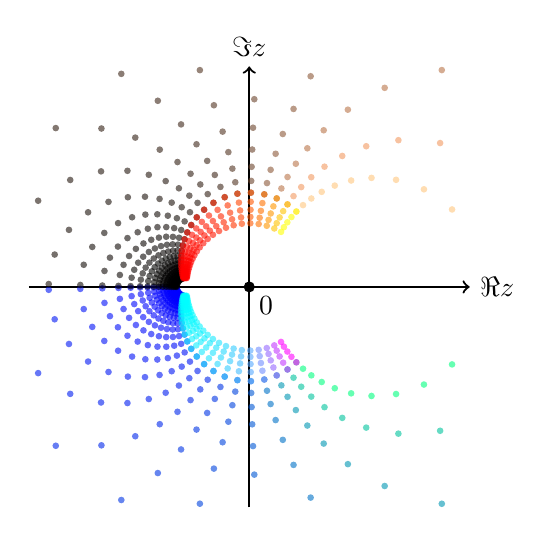
\begin{tikzpicture}[scale=0.8]

\draw[->, thick] (-3.5,0) -- (3.5,0) node[right] {$\Re z$};
\draw[->, thick] (0,-3.5) -- (0,3.5) node[above] {$\Im z$};

\fill (0,0) circle (2.5pt) node[below right] {$0$};

\fill[color={rgb,255:red,0; green,0; blue,255}, opacity=0.60] (-1.1758,-0.0019) circle (1.5pt);
\fill[color={rgb,255:red,0; green,0; blue,255}, opacity=0.60] (-1.2034,-0.0022) circle (1.5pt);
\fill[color={rgb,255:red,0; green,0; blue,255}, opacity=0.60] (-1.2358,-0.0026) circle (1.5pt);
\fill[color={rgb,255:red,0; green,0; blue,255}, opacity=0.60] (-1.2740,-0.0031) circle (1.5pt);
\fill[color={rgb,255:red,0; green,1; blue,254}, opacity=0.60] (-1.3193,-0.0037) circle (1.5pt);
\fill[color={rgb,255:red,0; green,1; blue,254}, opacity=0.60] (-1.3733,-0.0044) circle (1.5pt);
\fill[color={rgb,255:red,0; green,2; blue,254}, opacity=0.60] (-1.4382,-0.0053) circle (1.5pt);
\fill[color={rgb,255:red,0; green,3; blue,253}, opacity=0.60] (-1.5168,-0.0065) circle (1.5pt);
\fill[color={rgb,255:red,0; green,4; blue,253}, opacity=0.60] (-1.6131,-0.0080) circle (1.5pt);
\fill[color={rgb,255:red,0; green,5; blue,252}, opacity=0.60] (-1.7325,-0.0100) circle (1.5pt);
\fill[color={rgb,255:red,0; green,7; blue,251}, opacity=0.60] (-1.8830,-0.0127) circle (1.5pt);
\fill[color={rgb,255:red,0; green,10; blue,250}, opacity=0.60] (-2.0766,-0.0166) circle (1.5pt);
\fill[color={rgb,255:red,0; green,13; blue,248}, opacity=0.60] (-2.3323,-0.0222) circle (1.5pt);
\fill[color={rgb,255:red,0; green,17; blue,246}, opacity=0.60] (-2.6818,-0.0310) circle (1.5pt);
\fill[color={rgb,255:red,0; green,22; blue,244}, opacity=0.60] (-3.1832,-0.0457) circle (1.5pt);
\fill[color={rgb,255:red,0; green,0; blue,255}, opacity=0.60] (-1.1509,-0.0190) circle (1.5pt);
\fill[color={rgb,255:red,0; green,0; blue,255}, opacity=0.60] (-1.1743,-0.0221) circle (1.5pt);
\fill[color={rgb,255:red,0; green,0; blue,255}, opacity=0.60] (-1.2016,-0.0259) circle (1.5pt);
\fill[color={rgb,255:red,0; green,0; blue,255}, opacity=0.60] (-1.2336,-0.0305) circle (1.5pt);
\fill[color={rgb,255:red,0; green,0; blue,255}, opacity=0.60] (-1.2714,-0.0360) circle (1.5pt);
\fill[color={rgb,255:red,0; green,1; blue,254}, opacity=0.60] (-1.3160,-0.0428) circle (1.5pt);
\fill[color={rgb,255:red,0; green,1; blue,254}, opacity=0.60] (-1.3693,-0.0512) circle (1.5pt);
\fill[color={rgb,255:red,0; green,2; blue,254}, opacity=0.60] (-1.4331,-0.0617) circle (1.5pt);
\fill[color={rgb,255:red,0; green,3; blue,253}, opacity=0.60] (-1.5102,-0.0751) circle (1.5pt);
\fill[color={rgb,255:red,0; green,4; blue,253}, opacity=0.60] (-1.6045,-0.0924) circle (1.5pt);
\fill[color={rgb,255:red,0; green,5; blue,252}, opacity=0.60] (-1.7209,-0.1153) circle (1.5pt);
\fill[color={rgb,255:red,0; green,7; blue,251}, opacity=0.60] (-1.8671,-0.1463) circle (1.5pt);
\fill[color={rgb,255:red,0; green,10; blue,250}, opacity=0.60] (-2.0538,-0.1899) circle (1.5pt);
\fill[color={rgb,255:red,0; green,13; blue,248}, opacity=0.60] (-2.2981,-0.2536) circle (1.5pt);
\fill[color={rgb,255:red,0; green,17; blue,246}, opacity=0.60] (-2.6274,-0.3517) circle (1.5pt);
\fill[color={rgb,255:red,0; green,22; blue,244}, opacity=0.60] (-3.0888,-0.5138) circle (1.5pt);
\fill[color={rgb,255:red,0; green,0; blue,255}, opacity=0.60] (-1.1476,-0.0360) circle (1.5pt);
\fill[color={rgb,255:red,0; green,0; blue,255}, opacity=0.60] (-1.1703,-0.0420) circle (1.5pt);
\fill[color={rgb,255:red,0; green,0; blue,255}, opacity=0.60] (-1.1968,-0.0491) circle (1.5pt);
\fill[color={rgb,255:red,0; green,0; blue,255}, opacity=0.60] (-1.2278,-0.0578) circle (1.5pt);
\fill[color={rgb,255:red,0; green,0; blue,255}, opacity=0.60] (-1.2643,-0.0682) circle (1.5pt);
\fill[color={rgb,255:red,0; green,1; blue,254}, opacity=0.60] (-1.3074,-0.0809) circle (1.5pt);
\fill[color={rgb,255:red,0; green,1; blue,254}, opacity=0.60] (-1.3585,-0.0967) circle (1.5pt);
\fill[color={rgb,255:red,0; green,2; blue,254}, opacity=0.60] (-1.4196,-0.1163) circle (1.5pt);
\fill[color={rgb,255:red,0; green,3; blue,253}, opacity=0.60] (-1.4929,-0.1412) circle (1.5pt);
\fill[color={rgb,255:red,0; green,4; blue,253}, opacity=0.60] (-1.5819,-0.1733) circle (1.5pt);
\fill[color={rgb,255:red,0; green,5; blue,252}, opacity=0.60] (-1.6909,-0.2154) circle (1.5pt);
\fill[color={rgb,255:red,0; green,7; blue,251}, opacity=0.60] (-1.8258,-0.2722) circle (1.5pt);
\fill[color={rgb,255:red,0; green,10; blue,250}, opacity=0.60] (-1.9954,-0.3510) circle (1.5pt);
\fill[color={rgb,255:red,0; green,13; blue,248}, opacity=0.60] (-2.2116,-0.4643) circle (1.5pt);
\fill[color={rgb,255:red,0; green,17; blue,246}, opacity=0.60] (-2.4922,-0.6347) circle (1.5pt);
\fill[color={rgb,255:red,0; green,22; blue,244}, opacity=0.60] (-2.8620,-0.9058) circle (1.5pt);
\fill[color={rgb,255:red,0; green,29; blue,240}, opacity=0.60] (-3.3511,-1.3683) circle (1.5pt);
\fill[color={rgb,255:red,0; green,255; blue,127}, opacity=0.60] (3.2196,-1.2299) circle (1.5pt);
\fill[color={rgb,255:red,0; green,0; blue,255}, opacity=0.60] (-1.1422,-0.0524) circle (1.5pt);
\fill[color={rgb,255:red,0; green,0; blue,255}, opacity=0.60] (-1.1639,-0.0611) circle (1.5pt);
\fill[color={rgb,255:red,0; green,0; blue,255}, opacity=0.60] (-1.1891,-0.0715) circle (1.5pt);
\fill[color={rgb,255:red,0; green,0; blue,255}, opacity=0.60] (-1.2186,-0.0839) circle (1.5pt);
\fill[color={rgb,255:red,0; green,0; blue,255}, opacity=0.60] (-1.2531,-0.0989) circle (1.5pt);
\fill[color={rgb,255:red,0; green,1; blue,254}, opacity=0.60] (-1.2937,-0.1172) circle (1.5pt);
\fill[color={rgb,255:red,0; green,1; blue,254}, opacity=0.60] (-1.3416,-0.1397) circle (1.5pt);
\fill[color={rgb,255:red,0; green,2; blue,254}, opacity=0.60] (-1.3983,-0.1676) circle (1.5pt);
\fill[color={rgb,255:red,0; green,3; blue,253}, opacity=0.60] (-1.4659,-0.2028) circle (1.5pt);
\fill[color={rgb,255:red,0; green,4; blue,253}, opacity=0.60] (-1.5468,-0.2479) circle (1.5pt);
\fill[color={rgb,255:red,0; green,5; blue,252}, opacity=0.60] (-1.6445,-0.3066) circle (1.5pt);
\fill[color={rgb,255:red,0; green,7; blue,251}, opacity=0.60] (-1.7630,-0.3846) circle (1.5pt);
\fill[color={rgb,255:red,0; green,10; blue,250}, opacity=0.60] (-1.9077,-0.4910) circle (1.5pt);
\fill[color={rgb,255:red,0; green,13; blue,248}, opacity=0.60] (-2.0849,-0.6404) circle (1.5pt);
\fill[color={rgb,255:red,0; green,17; blue,246}, opacity=0.60] (-2.3010,-0.8574) circle (1.5pt);
\fill[color={rgb,255:red,0; green,22; blue,244}, opacity=0.60] (-2.5586,-1.1847) circle (1.5pt);
\fill[color={rgb,255:red,0; green,29; blue,240}, opacity=0.60] (-2.8421,-1.6978) circle (1.5pt);
\fill[color={rgb,255:red,0; green,39; blue,235}, opacity=0.60] (-3.0715,-2.5216) circle (1.5pt);
\fill[color={rgb,255:red,0; green,150; blue,179}, opacity=0.60] (3.0568,-3.4424) circle (1.5pt);
\fill[color={rgb,255:red,0; green,195; blue,157}, opacity=0.60] (3.0301,-2.2838) circle (1.5pt);
\fill[color={rgb,255:red,0; green,255; blue,127}, opacity=0.60] (2.7731,-1.5499) circle (1.5pt);
\fill[color={rgb,255:red,0; green,0; blue,255}, opacity=0.60] (-1.1349,-0.0679) circle (1.5pt);
\fill[color={rgb,255:red,0; green,0; blue,255}, opacity=0.60] (-1.1552,-0.0791) circle (1.5pt);
\fill[color={rgb,255:red,0; green,0; blue,255}, opacity=0.60] (-1.1788,-0.0925) circle (1.5pt);
\fill[color={rgb,255:red,0; green,0; blue,255}, opacity=0.60] (-1.2062,-0.1084) circle (1.5pt);
\fill[color={rgb,255:red,0; green,0; blue,255}, opacity=0.60] (-1.2381,-0.1275) circle (1.5pt);
\fill[color={rgb,255:red,0; green,1; blue,254}, opacity=0.60] (-1.2754,-0.1508) circle (1.5pt);
\fill[color={rgb,255:red,0; green,1; blue,254}, opacity=0.60] (-1.3190,-0.1792) circle (1.5pt);
\fill[color={rgb,255:red,0; green,2; blue,254}, opacity=0.60] (-1.3701,-0.2144) circle (1.5pt);
\fill[color={rgb,255:red,0; green,3; blue,253}, opacity=0.60] (-1.4303,-0.2583) circle (1.5pt);
\fill[color={rgb,255:red,0; green,4; blue,253}, opacity=0.60] (-1.5012,-0.3140) circle (1.5pt);
\fill[color={rgb,255:red,0; green,5; blue,252}, opacity=0.60] (-1.5850,-0.3856) circle (1.5pt);
\fill[color={rgb,255:red,0; green,7; blue,251}, opacity=0.60] (-1.6837,-0.4794) circle (1.5pt);
\fill[color={rgb,255:red,0; green,10; blue,250}, opacity=0.60] (-1.7995,-0.6045) circle (1.5pt);
\fill[color={rgb,255:red,0; green,13; blue,248}, opacity=0.60] (-1.9332,-0.7751) circle (1.5pt);
\fill[color={rgb,255:red,0; green,17; blue,246}, opacity=0.60] (-2.0823,-1.0127) circle (1.5pt);
\fill[color={rgb,255:red,0; green,22; blue,244}, opacity=0.60] (-2.2343,-1.3504) circle (1.5pt);
\fill[color={rgb,255:red,0; green,29; blue,240}, opacity=0.60] (-2.3527,-1.8345) circle (1.5pt);
\fill[color={rgb,255:red,0; green,39; blue,235}, opacity=0.60] (-2.3466,-2.5146) circle (1.5pt);
\fill[color={rgb,255:red,0; green,51; blue,229}, opacity=0.60] (-2.0312,-3.3825) circle (1.5pt);
\fill[color={rgb,255:red,0; green,150; blue,179}, opacity=0.60] (2.1501,-3.1603) circle (1.5pt);
\fill[color={rgb,255:red,0; green,195; blue,157}, opacity=0.60] (2.3677,-2.3292) circle (1.5pt);
\fill[color={rgb,255:red,0; green,255; blue,127}, opacity=0.60] (2.3306,-1.7002) circle (1.5pt);
\fill[color={rgb,255:red,0; green,0; blue,255}, opacity=0.60] (-1.1259,-0.0824) circle (1.5pt);
\fill[color={rgb,255:red,0; green,0; blue,255}, opacity=0.60] (-1.1445,-0.0959) circle (1.5pt);
\fill[color={rgb,255:red,0; green,0; blue,255}, opacity=0.60] (-1.1661,-0.1118) circle (1.5pt);
\fill[color={rgb,255:red,0; green,0; blue,255}, opacity=0.60] (-1.1910,-0.1308) circle (1.5pt);
\fill[color={rgb,255:red,0; green,0; blue,255}, opacity=0.60] (-1.2198,-0.1536) circle (1.5pt);
\fill[color={rgb,255:red,0; green,1; blue,254}, opacity=0.60] (-1.2531,-0.1811) circle (1.5pt);
\fill[color={rgb,255:red,0; green,1; blue,254}, opacity=0.60] (-1.2916,-0.2146) circle (1.5pt);
\fill[color={rgb,255:red,0; green,2; blue,254}, opacity=0.60] (-1.3363,-0.2556) circle (1.5pt);
\fill[color={rgb,255:red,0; green,3; blue,253}, opacity=0.60] (-1.3880,-0.3065) circle (1.5pt);
\fill[color={rgb,255:red,0; green,4; blue,253}, opacity=0.60] (-1.4476,-0.3702) circle (1.5pt);
\fill[color={rgb,255:red,0; green,5; blue,252}, opacity=0.60] (-1.5159,-0.4510) circle (1.5pt);
\fill[color={rgb,255:red,0; green,7; blue,251}, opacity=0.60] (-1.5935,-0.5547) circle (1.5pt);
\fill[color={rgb,255:red,0; green,10; blue,250}, opacity=0.60] (-1.6795,-0.6898) circle (1.5pt);
\fill[color={rgb,255:red,0; green,13; blue,248}, opacity=0.60] (-1.7711,-0.8681) circle (1.5pt);
\fill[color={rgb,255:red,0; green,17; blue,246}, opacity=0.60] (-1.8598,-1.1059) circle (1.5pt);
\fill[color={rgb,255:red,0; green,22; blue,244}, opacity=0.60] (-1.9269,-1.4239) circle (1.5pt);
\fill[color={rgb,255:red,0; green,29; blue,240}, opacity=0.60] (-1.9337,-1.8434) circle (1.5pt);
\fill[color={rgb,255:red,0; green,39; blue,235}, opacity=0.60] (-1.8092,-2.3703) circle (1.5pt);
\fill[color={rgb,255:red,0; green,51; blue,229}, opacity=0.60] (-1.4514,-2.9549) circle (1.5pt);
\fill[color={rgb,255:red,0; green,67; blue,221}, opacity=0.60] (-0.7839,-3.4413) circle (1.5pt);
\fill[color={rgb,255:red,0; green,113; blue,198}, opacity=0.60] (0.9745,-3.3443) circle (1.5pt);
\fill[color={rgb,255:red,0; green,150; blue,179}, opacity=0.60] (1.5656,-2.8135) circle (1.5pt);
\fill[color={rgb,255:red,0; green,195; blue,157}, opacity=0.60] (1.8568,-2.2333) circle (1.5pt);
\fill[color={rgb,255:red,0; green,255; blue,127}, opacity=0.60] (1.9408,-1.7310) circle (1.5pt);
\fill[color={rgb,255:red,0; green,0; blue,255}, opacity=0.60] (-1.1153,-0.0956) circle (1.5pt);
\fill[color={rgb,255:red,0; green,0; blue,255}, opacity=0.60] (-1.1320,-0.1110) circle (1.5pt);
\fill[color={rgb,255:red,0; green,0; blue,255}, opacity=0.60] (-1.1512,-0.1292) circle (1.5pt);
\fill[color={rgb,255:red,0; green,0; blue,255}, opacity=0.60] (-1.1733,-0.1509) circle (1.5pt);
\fill[color={rgb,255:red,0; green,0; blue,255}, opacity=0.60] (-1.1985,-0.1767) circle (1.5pt);
\fill[color={rgb,255:red,0; green,1; blue,254}, opacity=0.60] (-1.2274,-0.2077) circle (1.5pt);
\fill[color={rgb,255:red,0; green,1; blue,254}, opacity=0.60] (-1.2604,-0.2452) circle (1.5pt);
\fill[color={rgb,255:red,0; green,2; blue,254}, opacity=0.60] (-1.2980,-0.2907) circle (1.5pt);
\fill[color={rgb,255:red,0; green,3; blue,253}, opacity=0.60] (-1.3406,-0.3466) circle (1.5pt);
\fill[color={rgb,255:red,0; green,4; blue,253}, opacity=0.60] (-1.3883,-0.4157) circle (1.5pt);
\fill[color={rgb,255:red,0; green,5; blue,252}, opacity=0.60] (-1.4409,-0.5019) circle (1.5pt);
\fill[color={rgb,255:red,0; green,7; blue,251}, opacity=0.60] (-1.4976,-0.6104) circle (1.5pt);
\fill[color={rgb,255:red,0; green,10; blue,250}, opacity=0.60] (-1.5557,-0.7481) circle (1.5pt);
\fill[color={rgb,255:red,0; green,13; blue,248}, opacity=0.60] (-1.6098,-0.9239) circle (1.5pt);
\fill[color={rgb,255:red,0; green,17; blue,246}, opacity=0.60] (-1.6494,-1.1483) circle (1.5pt);
\fill[color={rgb,255:red,0; green,22; blue,244}, opacity=0.60] (-1.6551,-1.4319) circle (1.5pt);
\fill[color={rgb,255:red,0; green,29; blue,240}, opacity=0.60] (-1.5946,-1.7798) circle (1.5pt);
\fill[color={rgb,255:red,0; green,39; blue,235}, opacity=0.60] (-1.4207,-2.1792) circle (1.5pt);
\fill[color={rgb,255:red,0; green,51; blue,229}, opacity=0.60] (-1.0824,-2.5800) circle (1.5pt);
\fill[color={rgb,255:red,0; green,67; blue,221}, opacity=0.60] (-0.5612,-2.8841) circle (1.5pt);
\fill[color={rgb,255:red,0; green,87; blue,211}, opacity=0.60] (0.0802,-2.9799) circle (1.5pt);
\fill[color={rgb,255:red,0; green,113; blue,198}, opacity=0.60] (0.7032,-2.8254) circle (1.5pt);
\fill[color={rgb,255:red,0; green,150; blue,179}, opacity=0.60] (1.1820,-2.4869) circle (1.5pt);
\fill[color={rgb,255:red,0; green,195; blue,157}, opacity=0.60] (1.4764,-2.0791) circle (1.5pt);
\fill[color={rgb,255:red,0; green,255; blue,127}, opacity=0.60] (1.6177,-1.6893) circle (1.5pt);
\fill[color={rgb,255:red,0; green,0; blue,255}, opacity=0.60] (-1.1033,-0.1073) circle (1.5pt);
\fill[color={rgb,255:red,0; green,0; blue,255}, opacity=0.60] (-1.1179,-0.1244) circle (1.5pt);
\fill[color={rgb,255:red,0; green,0; blue,255}, opacity=0.60] (-1.1346,-0.1445) circle (1.5pt);
\fill[color={rgb,255:red,0; green,0; blue,255}, opacity=0.60] (-1.1535,-0.1683) circle (1.5pt);
\fill[color={rgb,255:red,0; green,0; blue,255}, opacity=0.60] (-1.1750,-0.1966) circle (1.5pt);
\fill[color={rgb,255:red,0; green,1; blue,254}, opacity=0.60] (-1.1992,-0.2303) circle (1.5pt);
\fill[color={rgb,255:red,0; green,1; blue,254}, opacity=0.60] (-1.2263,-0.2706) circle (1.5pt);
\fill[color={rgb,255:red,0; green,2; blue,254}, opacity=0.60] (-1.2566,-0.3193) circle (1.5pt);
\fill[color={rgb,255:red,0; green,3; blue,253}, opacity=0.60] (-1.2898,-0.3784) circle (1.5pt);
\fill[color={rgb,255:red,0; green,4; blue,253}, opacity=0.60] (-1.3257,-0.4504) circle (1.5pt);
\fill[color={rgb,255:red,0; green,5; blue,252}, opacity=0.60] (-1.3633,-0.5388) circle (1.5pt);
\fill[color={rgb,255:red,0; green,7; blue,251}, opacity=0.60] (-1.4006,-0.6477) circle (1.5pt);
\fill[color={rgb,255:red,0; green,10; blue,250}, opacity=0.60] (-1.4340,-0.7824) circle (1.5pt);
\fill[color={rgb,255:red,0; green,13; blue,248}, opacity=0.60] (-1.4571,-0.9488) circle (1.5pt);
\fill[color={rgb,255:red,0; green,17; blue,246}, opacity=0.60] (-1.4593,-1.1527) circle (1.5pt);
\fill[color={rgb,255:red,0; green,22; blue,244}, opacity=0.60] (-1.4238,-1.3976) circle (1.5pt);
\fill[color={rgb,255:red,0; green,29; blue,240}, opacity=0.60] (-1.3267,-1.6801) circle (1.5pt);
\fill[color={rgb,255:red,0; green,39; blue,235}, opacity=0.60] (-1.1391,-1.9825) circle (1.5pt);
\fill[color={rgb,255:red,0; green,51; blue,229}, opacity=0.60] (-0.8373,-2.2646) circle (1.5pt);
\fill[color={rgb,255:red,0; green,67; blue,221}, opacity=0.60] (-0.4228,-2.4656) circle (1.5pt);
\fill[color={rgb,255:red,0; green,87; blue,211}, opacity=0.60] (0.0599,-2.5269) circle (1.5pt);
\fill[color={rgb,255:red,0; green,113; blue,198}, opacity=0.60] (0.5325,-2.4277) circle (1.5pt);
\fill[color={rgb,255:red,0; green,150; blue,179}, opacity=0.60] (0.9219,-2.2008) circle (1.5pt);
\fill[color={rgb,255:red,0; green,195; blue,157}, opacity=0.60] (1.1946,-1.9088) circle (1.5pt);
\fill[color={rgb,255:red,0; green,255; blue,127}, opacity=0.60] (1.3575,-1.6085) circle (1.5pt);
\fill[color={rgb,255:red,0; green,0; blue,255}, opacity=0.60] (-1.0902,-0.1174) circle (1.5pt);
\fill[color={rgb,255:red,0; green,0; blue,255}, opacity=0.60] (-1.1026,-0.1358) circle (1.5pt);
\fill[color={rgb,255:red,0; green,0; blue,255}, opacity=0.60] (-1.1165,-0.1575) circle (1.5pt);
\fill[color={rgb,255:red,0; green,0; blue,255}, opacity=0.60] (-1.1322,-0.1829) circle (1.5pt);
\fill[color={rgb,255:red,0; green,0; blue,255}, opacity=0.60] (-1.1497,-0.2130) circle (1.5pt);
\fill[color={rgb,255:red,0; green,1; blue,254}, opacity=0.60] (-1.1690,-0.2486) circle (1.5pt);
\fill[color={rgb,255:red,0; green,1; blue,254}, opacity=0.60] (-1.1903,-0.2909) circle (1.5pt);
\fill[color={rgb,255:red,0; green,2; blue,254}, opacity=0.60] (-1.2132,-0.3414) circle (1.5pt);
\fill[color={rgb,255:red,0; green,3; blue,253}, opacity=0.60] (-1.2374,-0.4019) circle (1.5pt);
\fill[color={rgb,255:red,0; green,4; blue,253}, opacity=0.60] (-1.2621,-0.4748) circle (1.5pt);
\fill[color={rgb,255:red,0; green,5; blue,252}, opacity=0.60] (-1.2857,-0.5627) circle (1.5pt);
\fill[color={rgb,255:red,0; green,7; blue,251}, opacity=0.60] (-1.3059,-0.6688) circle (1.5pt);
\fill[color={rgb,255:red,0; green,10; blue,250}, opacity=0.60] (-1.3185,-0.7966) circle (1.5pt);
\fill[color={rgb,255:red,0; green,13; blue,248}, opacity=0.60] (-1.3171,-0.9498) circle (1.5pt);
\fill[color={rgb,255:red,0; green,17; blue,246}, opacity=0.60] (-1.2924,-1.1305) circle (1.5pt);
\fill[color={rgb,255:red,0; green,22; blue,244}, opacity=0.60] (-1.2311,-1.3382) circle (1.5pt);
\fill[color={rgb,255:red,0; green,29; blue,240}, opacity=0.60] (-1.1166,-1.5659) circle (1.5pt);
\fill[color={rgb,255:red,0; green,39; blue,235}, opacity=0.60] (-0.9321,-1.7965) circle (1.5pt);
\fill[color={rgb,255:red,0; green,51; blue,229}, opacity=0.60] (-0.6679,-2.0004) circle (1.5pt);
\fill[color={rgb,255:red,0; green,67; blue,221}, opacity=0.60] (-0.3313,-2.1396) circle (1.5pt);
\fill[color={rgb,255:red,0; green,87; blue,211}, opacity=0.60] (0.0467,-2.1810) circle (1.5pt);
\fill[color={rgb,255:red,0; green,113; blue,198}, opacity=0.60] (0.4187,-2.1137) circle (1.5pt);
\fill[color={rgb,255:red,0; green,150; blue,179}, opacity=0.60] (0.7396,-1.9552) circle (1.5pt);
\fill[color={rgb,255:red,0; green,195; blue,157}, opacity=0.60] (0.9842,-1.7414) circle (1.5pt);
\fill[color={rgb,255:red,0; green,255; blue,127}, opacity=0.60] (1.1503,-1.5093) circle (1.5pt);
\fill[color={rgb,255:red,0; green,0; blue,255}, opacity=0.60] (-1.0762,-0.1258) circle (1.5pt);
\fill[color={rgb,255:red,0; green,0; blue,255}, opacity=0.60] (-1.0862,-0.1453) circle (1.5pt);
\fill[color={rgb,255:red,0; green,0; blue,255}, opacity=0.60] (-1.0974,-0.1681) circle (1.5pt);
\fill[color={rgb,255:red,0; green,0; blue,255}, opacity=0.60] (-1.1097,-0.1947) circle (1.5pt);
\fill[color={rgb,255:red,0; green,0; blue,255}, opacity=0.60] (-1.1231,-0.2259) circle (1.5pt);
\fill[color={rgb,255:red,0; green,1; blue,254}, opacity=0.60] (-1.1377,-0.2626) circle (1.5pt);
\fill[color={rgb,255:red,0; green,1; blue,254}, opacity=0.60] (-1.1531,-0.3059) circle (1.5pt);
\fill[color={rgb,255:red,0; green,2; blue,254}, opacity=0.60] (-1.1690,-0.3571) circle (1.5pt);
\fill[color={rgb,255:red,0; green,3; blue,253}, opacity=0.60] (-1.1846,-0.4178) circle (1.5pt);
\fill[color={rgb,255:red,0; green,4; blue,253}, opacity=0.60] (-1.1990,-0.4897) circle (1.5pt);
\fill[color={rgb,255:red,0; green,5; blue,252}, opacity=0.60] (-1.2103,-0.5750) circle (1.5pt);
\fill[color={rgb,255:red,0; green,7; blue,251}, opacity=0.60] (-1.2158,-0.6760) circle (1.5pt);
\fill[color={rgb,255:red,0; green,10; blue,250}, opacity=0.60] (-1.2115,-0.7947) circle (1.5pt);
\fill[color={rgb,255:red,0; green,13; blue,248}, opacity=0.60] (-1.1917,-0.9330) circle (1.5pt);
\fill[color={rgb,255:red,0; green,17; blue,246}, opacity=0.60] (-1.1485,-1.0907) circle (1.5pt);
\fill[color={rgb,255:red,0; green,22; blue,244}, opacity=0.60] (-1.0721,-1.2652) circle (1.5pt);
\fill[color={rgb,255:red,0; green,29; blue,240}, opacity=0.60] (-0.9514,-1.4487) circle (1.5pt);
\fill[color={rgb,255:red,0; green,39; blue,235}, opacity=0.60] (-0.7773,-1.6265) circle (1.5pt);
\fill[color={rgb,255:red,0; green,51; blue,229}, opacity=0.60] (-0.5467,-1.7777) circle (1.5pt);
\fill[color={rgb,255:red,0; green,67; blue,221}, opacity=0.60] (-0.2678,-1.8776) circle (1.5pt);
\fill[color={rgb,255:red,0; green,87; blue,211}, opacity=0.60] (0.0376,-1.9069) circle (1.5pt);
\fill[color={rgb,255:red,0; green,113; blue,198}, opacity=0.60] (0.3392,-1.8592) circle (1.5pt);
\fill[color={rgb,255:red,0; green,150; blue,179}, opacity=0.60] (0.6078,-1.7446) circle (1.5pt);
\fill[color={rgb,255:red,0; green,195; blue,157}, opacity=0.60] (0.8250,-1.5848) circle (1.5pt);
\fill[color={rgb,255:red,0; green,255; blue,127}, opacity=0.60] (0.9855,-1.4038) circle (1.5pt);
\fill[color={rgb,255:red,0; green,0; blue,255}, opacity=0.60] (-1.0615,-0.1325) circle (1.5pt);
\fill[color={rgb,255:red,0; green,0; blue,255}, opacity=0.60] (-1.0691,-0.1527) circle (1.5pt);
\fill[color={rgb,255:red,0; green,0; blue,255}, opacity=0.60] (-1.0775,-0.1762) circle (1.5pt);
\fill[color={rgb,255:red,0; green,0; blue,255}, opacity=0.60] (-1.0864,-0.2035) circle (1.5pt);
\fill[color={rgb,255:red,0; green,0; blue,255}, opacity=0.60] (-1.0959,-0.2354) circle (1.5pt);
\fill[color={rgb,255:red,0; green,1; blue,254}, opacity=0.60] (-1.1058,-0.2725) circle (1.5pt);
\fill[color={rgb,255:red,0; green,1; blue,254}, opacity=0.60] (-1.1156,-0.3160) circle (1.5pt);
\fill[color={rgb,255:red,0; green,2; blue,254}, opacity=0.60] (-1.1248,-0.3669) circle (1.5pt);
\fill[color={rgb,255:red,0; green,3; blue,253}, opacity=0.60] (-1.1326,-0.4265) circle (1.5pt);
\fill[color={rgb,255:red,0; green,4; blue,253}, opacity=0.60] (-1.1378,-0.4961) circle (1.5pt);
\fill[color={rgb,255:red,0; green,5; blue,252}, opacity=0.60] (-1.1383,-0.5774) circle (1.5pt);
\fill[color={rgb,255:red,0; green,7; blue,251}, opacity=0.60] (-1.1317,-0.6718) circle (1.5pt);
\fill[color={rgb,255:red,0; green,10; blue,250}, opacity=0.60] (-1.1142,-0.7804) circle (1.5pt);
\fill[color={rgb,255:red,0; green,13; blue,248}, opacity=0.60] (-1.0809,-0.9035) circle (1.5pt);
\fill[color={rgb,255:red,0; green,17; blue,246}, opacity=0.60] (-1.0256,-1.0399) circle (1.5pt);
\fill[color={rgb,255:red,0; green,22; blue,244}, opacity=0.60] (-0.9412,-1.1860) circle (1.5pt);
\fill[color={rgb,255:red,0; green,29; blue,240}, opacity=0.60] (-0.8208,-1.3343) circle (1.5pt);
\fill[color={rgb,255:red,0; green,39; blue,235}, opacity=0.60] (-0.6595,-1.4733) circle (1.5pt);
\fill[color={rgb,255:red,0; green,51; blue,229}, opacity=0.60] (-0.4573,-1.5878) circle (1.5pt);
\fill[color={rgb,255:red,0; green,67; blue,221}, opacity=0.60] (-0.2220,-1.6618) circle (1.5pt);
\fill[color={rgb,255:red,0; green,87; blue,211}, opacity=0.60] (0.0311,-1.6832) circle (1.5pt);
\fill[color={rgb,255:red,0; green,113; blue,198}, opacity=0.60] (0.2817,-1.6483) circle (1.5pt);
\fill[color={rgb,255:red,0; green,150; blue,179}, opacity=0.60] (0.5101,-1.5631) circle (1.5pt);
\fill[color={rgb,255:red,0; green,195; blue,157}, opacity=0.60] (0.7026,-1.4411) circle (1.5pt);
\fill[color={rgb,255:red,0; green,255; blue,127}, opacity=0.60] (0.8538,-1.2985) circle (1.5pt);
\fill[color={rgb,255:red,0; green,0; blue,255}, opacity=0.60] (-1.0464,-0.1374) circle (1.5pt);
\fill[color={rgb,255:red,0; green,0; blue,255}, opacity=0.60] (-1.0516,-0.1580) circle (1.5pt);
\fill[color={rgb,255:red,0; green,0; blue,255}, opacity=0.60] (-1.0572,-0.1819) circle (1.5pt);
\fill[color={rgb,255:red,0; green,0; blue,255}, opacity=0.60] (-1.0628,-0.2095) circle (1.5pt);
\fill[color={rgb,255:red,0; green,0; blue,255}, opacity=0.60] (-1.0685,-0.2414) circle (1.5pt);
\fill[color={rgb,255:red,0; green,1; blue,254}, opacity=0.60] (-1.0738,-0.2785) circle (1.5pt);
\fill[color={rgb,255:red,0; green,1; blue,254}, opacity=0.60] (-1.0784,-0.3214) circle (1.5pt);
\fill[color={rgb,255:red,0; green,2; blue,254}, opacity=0.60] (-1.0815,-0.3712) circle (1.5pt);
\fill[color={rgb,255:red,0; green,3; blue,253}, opacity=0.60] (-1.0823,-0.4288) circle (1.5pt);
\fill[color={rgb,255:red,0; green,4; blue,253}, opacity=0.60] (-1.0794,-0.4952) circle (1.5pt);
\fill[color={rgb,255:red,0; green,5; blue,252}, opacity=0.60] (-1.0709,-0.5715) circle (1.5pt);
\fill[color={rgb,255:red,0; green,7; blue,251}, opacity=0.60] (-1.0544,-0.6586) circle (1.5pt);
\fill[color={rgb,255:red,0; green,10; blue,250}, opacity=0.60] (-1.0268,-0.7566) circle (1.5pt);
\fill[color={rgb,255:red,0; green,13; blue,248}, opacity=0.60] (-0.9839,-0.8653) circle (1.5pt);
\fill[color={rgb,255:red,0; green,17; blue,246}, opacity=0.60] (-0.9211,-0.9827) circle (1.5pt);
\fill[color={rgb,255:red,0; green,22; blue,244}, opacity=0.60] (-0.8334,-1.1049) circle (1.5pt);
\fill[color={rgb,255:red,0; green,29; blue,240}, opacity=0.60] (-0.7165,-1.2255) circle (1.5pt);
\fill[color={rgb,255:red,0; green,39; blue,235}, opacity=0.60] (-0.5682,-1.3355) circle (1.5pt);
\fill[color={rgb,255:red,0; green,51; blue,229}, opacity=0.60] (-0.3898,-1.4240) circle (1.5pt);
\fill[color={rgb,255:red,0; green,67; blue,221}, opacity=0.60] (-0.1879,-1.4802) circle (1.5pt);
\fill[color={rgb,255:red,0; green,87; blue,211}, opacity=0.60] (0.0263,-1.4963) circle (1.5pt);
\fill[color={rgb,255:red,0; green,113; blue,198}, opacity=0.60] (0.2387,-1.4699) circle (1.5pt);
\fill[color={rgb,255:red,0; green,150; blue,179}, opacity=0.60] (0.4358,-1.4050) circle (1.5pt);
\fill[color={rgb,255:red,0; green,195; blue,157}, opacity=0.60] (0.6072,-1.3103) circle (1.5pt);
\fill[color={rgb,255:red,0; green,255; blue,127}, opacity=0.60] (0.7478,-1.1967) circle (1.5pt);
\fill[color={rgb,255:red,0; green,0; blue,0}, opacity=0.60] (-1.0464,0.1374) circle (1.5pt);
\fill[color={rgb,255:red,0; green,0; blue,0}, opacity=0.60] (-1.0516,0.1580) circle (1.5pt);
\fill[color={rgb,255:red,0; green,0; blue,0}, opacity=0.60] (-1.0572,0.1819) circle (1.5pt);
\fill[color={rgb,255:red,0; green,0; blue,0}, opacity=0.60] (-1.0628,0.2095) circle (1.5pt);
\fill[color={rgb,255:red,0; green,0; blue,0}, opacity=0.60] (-1.0685,0.2414) circle (1.5pt);
\fill[color={rgb,255:red,1; green,0; blue,0}, opacity=0.60] (-1.0738,0.2785) circle (1.5pt);
\fill[color={rgb,255:red,1; green,0; blue,0}, opacity=0.60] (-1.0784,0.3214) circle (1.5pt);
\fill[color={rgb,255:red,2; green,1; blue,0}, opacity=0.60] (-1.0815,0.3712) circle (1.5pt);
\fill[color={rgb,255:red,3; green,2; blue,1}, opacity=0.60] (-1.0823,0.4288) circle (1.5pt);
\fill[color={rgb,255:red,4; green,3; blue,1}, opacity=0.60] (-1.0794,0.4952) circle (1.5pt);
\fill[color={rgb,255:red,6; green,3; blue,2}, opacity=0.60] (-1.0709,0.5715) circle (1.5pt);
\fill[color={rgb,255:red,8; green,5; blue,3}, opacity=0.60] (-1.0544,0.6586) circle (1.5pt);
\fill[color={rgb,255:red,12; green,7; blue,4}, opacity=0.60] (-1.0268,0.7566) circle (1.5pt);
\fill[color={rgb,255:red,16; green,10; blue,6}, opacity=0.60] (-0.9839,0.8653) circle (1.5pt);
\fill[color={rgb,255:red,20; green,13; blue,8}, opacity=0.60] (-0.9211,0.9827) circle (1.5pt);
\fill[color={rgb,255:red,27; green,17; blue,10}, opacity=0.60] (-0.8334,1.1049) circle (1.5pt);
\fill[color={rgb,255:red,35; green,22; blue,14}, opacity=0.60] (-0.7165,1.2255) circle (1.5pt);
\fill[color={rgb,255:red,48; green,30; blue,19}, opacity=0.60] (-0.5682,1.3355) circle (1.5pt);
\fill[color={rgb,255:red,62; green,39; blue,25}, opacity=0.60] (-0.3898,1.4240) circle (1.5pt);
\fill[color={rgb,255:red,82; green,52; blue,33}, opacity=0.60] (-0.1879,1.4802) circle (1.5pt);
\fill[color={rgb,255:red,107; green,67; blue,43}, opacity=0.60] (0.0263,1.4963) circle (1.5pt);
\fill[color={rgb,255:red,140; green,89; blue,56}, opacity=0.60] (0.2387,1.4699) circle (1.5pt);
\fill[color={rgb,255:red,185; green,117; blue,74}, opacity=0.60] (0.4358,1.4050) circle (1.5pt);
\fill[color={rgb,255:red,242; green,153; blue,97}, opacity=0.60] (0.6072,1.3103) circle (1.5pt);
\fill[color={rgb,255:red,255; green,199; blue,126}, opacity=0.60] (0.7478,1.1967) circle (1.5pt);
\fill[color={rgb,255:red,0; green,0; blue,0}, opacity=0.60] (-1.0615,0.1325) circle (1.5pt);
\fill[color={rgb,255:red,0; green,0; blue,0}, opacity=0.60] (-1.0691,0.1527) circle (1.5pt);
\fill[color={rgb,255:red,0; green,0; blue,0}, opacity=0.60] (-1.0775,0.1762) circle (1.5pt);
\fill[color={rgb,255:red,0; green,0; blue,0}, opacity=0.60] (-1.0864,0.2035) circle (1.5pt);
\fill[color={rgb,255:red,0; green,0; blue,0}, opacity=0.60] (-1.0959,0.2354) circle (1.5pt);
\fill[color={rgb,255:red,1; green,0; blue,0}, opacity=0.60] (-1.1058,0.2725) circle (1.5pt);
\fill[color={rgb,255:red,1; green,0; blue,0}, opacity=0.60] (-1.1156,0.3160) circle (1.5pt);
\fill[color={rgb,255:red,2; green,1; blue,0}, opacity=0.60] (-1.1248,0.3669) circle (1.5pt);
\fill[color={rgb,255:red,3; green,2; blue,1}, opacity=0.60] (-1.1326,0.4265) circle (1.5pt);
\fill[color={rgb,255:red,4; green,3; blue,1}, opacity=0.60] (-1.1378,0.4961) circle (1.5pt);
\fill[color={rgb,255:red,6; green,3; blue,2}, opacity=0.60] (-1.1383,0.5774) circle (1.5pt);
\fill[color={rgb,255:red,8; green,5; blue,3}, opacity=0.60] (-1.1317,0.6718) circle (1.5pt);
\fill[color={rgb,255:red,12; green,7; blue,4}, opacity=0.60] (-1.1142,0.7804) circle (1.5pt);
\fill[color={rgb,255:red,16; green,10; blue,6}, opacity=0.60] (-1.0809,0.9035) circle (1.5pt);
\fill[color={rgb,255:red,20; green,13; blue,8}, opacity=0.60] (-1.0256,1.0399) circle (1.5pt);
\fill[color={rgb,255:red,27; green,17; blue,10}, opacity=0.60] (-0.9412,1.1860) circle (1.5pt);
\fill[color={rgb,255:red,35; green,22; blue,14}, opacity=0.60] (-0.8208,1.3343) circle (1.5pt);
\fill[color={rgb,255:red,48; green,30; blue,19}, opacity=0.60] (-0.6595,1.4733) circle (1.5pt);
\fill[color={rgb,255:red,62; green,39; blue,25}, opacity=0.60] (-0.4573,1.5878) circle (1.5pt);
\fill[color={rgb,255:red,82; green,52; blue,33}, opacity=0.60] (-0.2220,1.6618) circle (1.5pt);
\fill[color={rgb,255:red,107; green,67; blue,43}, opacity=0.60] (0.0311,1.6832) circle (1.5pt);
\fill[color={rgb,255:red,140; green,89; blue,56}, opacity=0.60] (0.2817,1.6483) circle (1.5pt);
\fill[color={rgb,255:red,185; green,117; blue,74}, opacity=0.60] (0.5101,1.5631) circle (1.5pt);
\fill[color={rgb,255:red,242; green,153; blue,97}, opacity=0.60] (0.7026,1.4411) circle (1.5pt);
\fill[color={rgb,255:red,255; green,199; blue,126}, opacity=0.60] (0.8538,1.2985) circle (1.5pt);
\fill[color={rgb,255:red,0; green,0; blue,0}, opacity=0.60] (-1.0762,0.1258) circle (1.5pt);
\fill[color={rgb,255:red,0; green,0; blue,0}, opacity=0.60] (-1.0862,0.1453) circle (1.5pt);
\fill[color={rgb,255:red,0; green,0; blue,0}, opacity=0.60] (-1.0974,0.1681) circle (1.5pt);
\fill[color={rgb,255:red,0; green,0; blue,0}, opacity=0.60] (-1.1097,0.1947) circle (1.5pt);
\fill[color={rgb,255:red,0; green,0; blue,0}, opacity=0.60] (-1.1231,0.2259) circle (1.5pt);
\fill[color={rgb,255:red,1; green,0; blue,0}, opacity=0.60] (-1.1377,0.2626) circle (1.5pt);
\fill[color={rgb,255:red,1; green,0; blue,0}, opacity=0.60] (-1.1531,0.3059) circle (1.5pt);
\fill[color={rgb,255:red,2; green,1; blue,0}, opacity=0.60] (-1.1690,0.3571) circle (1.5pt);
\fill[color={rgb,255:red,3; green,2; blue,1}, opacity=0.60] (-1.1846,0.4178) circle (1.5pt);
\fill[color={rgb,255:red,4; green,3; blue,1}, opacity=0.60] (-1.1990,0.4897) circle (1.5pt);
\fill[color={rgb,255:red,6; green,3; blue,2}, opacity=0.60] (-1.2103,0.5750) circle (1.5pt);
\fill[color={rgb,255:red,8; green,5; blue,3}, opacity=0.60] (-1.2158,0.6760) circle (1.5pt);
\fill[color={rgb,255:red,12; green,7; blue,4}, opacity=0.60] (-1.2115,0.7947) circle (1.5pt);
\fill[color={rgb,255:red,16; green,10; blue,6}, opacity=0.60] (-1.1917,0.9330) circle (1.5pt);
\fill[color={rgb,255:red,20; green,13; blue,8}, opacity=0.60] (-1.1485,1.0907) circle (1.5pt);
\fill[color={rgb,255:red,27; green,17; blue,10}, opacity=0.60] (-1.0721,1.2652) circle (1.5pt);
\fill[color={rgb,255:red,35; green,22; blue,14}, opacity=0.60] (-0.9514,1.4487) circle (1.5pt);
\fill[color={rgb,255:red,48; green,30; blue,19}, opacity=0.60] (-0.7773,1.6265) circle (1.5pt);
\fill[color={rgb,255:red,62; green,39; blue,25}, opacity=0.60] (-0.5467,1.7777) circle (1.5pt);
\fill[color={rgb,255:red,82; green,52; blue,33}, opacity=0.60] (-0.2678,1.8776) circle (1.5pt);
\fill[color={rgb,255:red,107; green,67; blue,43}, opacity=0.60] (0.0376,1.9069) circle (1.5pt);
\fill[color={rgb,255:red,140; green,89; blue,56}, opacity=0.60] (0.3392,1.8592) circle (1.5pt);
\fill[color={rgb,255:red,185; green,117; blue,74}, opacity=0.60] (0.6078,1.7446) circle (1.5pt);
\fill[color={rgb,255:red,242; green,153; blue,97}, opacity=0.60] (0.8250,1.5848) circle (1.5pt);
\fill[color={rgb,255:red,255; green,199; blue,126}, opacity=0.60] (0.9855,1.4038) circle (1.5pt);
\fill[color={rgb,255:red,0; green,0; blue,0}, opacity=0.60] (-1.0902,0.1174) circle (1.5pt);
\fill[color={rgb,255:red,0; green,0; blue,0}, opacity=0.60] (-1.1026,0.1358) circle (1.5pt);
\fill[color={rgb,255:red,0; green,0; blue,0}, opacity=0.60] (-1.1165,0.1575) circle (1.5pt);
\fill[color={rgb,255:red,0; green,0; blue,0}, opacity=0.60] (-1.1322,0.1829) circle (1.5pt);
\fill[color={rgb,255:red,0; green,0; blue,0}, opacity=0.60] (-1.1497,0.2130) circle (1.5pt);
\fill[color={rgb,255:red,1; green,0; blue,0}, opacity=0.60] (-1.1690,0.2486) circle (1.5pt);
\fill[color={rgb,255:red,1; green,0; blue,0}, opacity=0.60] (-1.1903,0.2909) circle (1.5pt);
\fill[color={rgb,255:red,2; green,1; blue,0}, opacity=0.60] (-1.2132,0.3414) circle (1.5pt);
\fill[color={rgb,255:red,3; green,2; blue,1}, opacity=0.60] (-1.2374,0.4019) circle (1.5pt);
\fill[color={rgb,255:red,4; green,3; blue,1}, opacity=0.60] (-1.2621,0.4748) circle (1.5pt);
\fill[color={rgb,255:red,6; green,3; blue,2}, opacity=0.60] (-1.2857,0.5627) circle (1.5pt);
\fill[color={rgb,255:red,8; green,5; blue,3}, opacity=0.60] (-1.3059,0.6688) circle (1.5pt);
\fill[color={rgb,255:red,12; green,7; blue,4}, opacity=0.60] (-1.3185,0.7966) circle (1.5pt);
\fill[color={rgb,255:red,16; green,10; blue,6}, opacity=0.60] (-1.3171,0.9498) circle (1.5pt);
\fill[color={rgb,255:red,20; green,13; blue,8}, opacity=0.60] (-1.2924,1.1305) circle (1.5pt);
\fill[color={rgb,255:red,27; green,17; blue,10}, opacity=0.60] (-1.2311,1.3382) circle (1.5pt);
\fill[color={rgb,255:red,35; green,22; blue,14}, opacity=0.60] (-1.1166,1.5659) circle (1.5pt);
\fill[color={rgb,255:red,48; green,30; blue,19}, opacity=0.60] (-0.9321,1.7965) circle (1.5pt);
\fill[color={rgb,255:red,62; green,39; blue,25}, opacity=0.60] (-0.6679,2.0004) circle (1.5pt);
\fill[color={rgb,255:red,82; green,52; blue,33}, opacity=0.60] (-0.3313,2.1396) circle (1.5pt);
\fill[color={rgb,255:red,107; green,67; blue,43}, opacity=0.60] (0.0467,2.1810) circle (1.5pt);
\fill[color={rgb,255:red,140; green,89; blue,56}, opacity=0.60] (0.4187,2.1137) circle (1.5pt);
\fill[color={rgb,255:red,185; green,117; blue,74}, opacity=0.60] (0.7396,1.9552) circle (1.5pt);
\fill[color={rgb,255:red,242; green,153; blue,97}, opacity=0.60] (0.9842,1.7414) circle (1.5pt);
\fill[color={rgb,255:red,255; green,199; blue,126}, opacity=0.60] (1.1503,1.5093) circle (1.5pt);
\fill[color={rgb,255:red,0; green,0; blue,0}, opacity=0.60] (-1.1033,0.1073) circle (1.5pt);
\fill[color={rgb,255:red,0; green,0; blue,0}, opacity=0.60] (-1.1179,0.1244) circle (1.5pt);
\fill[color={rgb,255:red,0; green,0; blue,0}, opacity=0.60] (-1.1346,0.1445) circle (1.5pt);
\fill[color={rgb,255:red,0; green,0; blue,0}, opacity=0.60] (-1.1535,0.1683) circle (1.5pt);
\fill[color={rgb,255:red,0; green,0; blue,0}, opacity=0.60] (-1.1750,0.1966) circle (1.5pt);
\fill[color={rgb,255:red,1; green,0; blue,0}, opacity=0.60] (-1.1992,0.2303) circle (1.5pt);
\fill[color={rgb,255:red,1; green,0; blue,0}, opacity=0.60] (-1.2263,0.2706) circle (1.5pt);
\fill[color={rgb,255:red,2; green,1; blue,0}, opacity=0.60] (-1.2566,0.3193) circle (1.5pt);
\fill[color={rgb,255:red,3; green,2; blue,1}, opacity=0.60] (-1.2898,0.3784) circle (1.5pt);
\fill[color={rgb,255:red,4; green,3; blue,1}, opacity=0.60] (-1.3257,0.4504) circle (1.5pt);
\fill[color={rgb,255:red,6; green,3; blue,2}, opacity=0.60] (-1.3633,0.5388) circle (1.5pt);
\fill[color={rgb,255:red,8; green,5; blue,3}, opacity=0.60] (-1.4006,0.6477) circle (1.5pt);
\fill[color={rgb,255:red,12; green,7; blue,4}, opacity=0.60] (-1.4340,0.7824) circle (1.5pt);
\fill[color={rgb,255:red,16; green,10; blue,6}, opacity=0.60] (-1.4571,0.9488) circle (1.5pt);
\fill[color={rgb,255:red,20; green,13; blue,8}, opacity=0.60] (-1.4593,1.1527) circle (1.5pt);
\fill[color={rgb,255:red,27; green,17; blue,10}, opacity=0.60] (-1.4238,1.3976) circle (1.5pt);
\fill[color={rgb,255:red,35; green,22; blue,14}, opacity=0.60] (-1.3267,1.6801) circle (1.5pt);
\fill[color={rgb,255:red,48; green,30; blue,19}, opacity=0.60] (-1.1391,1.9825) circle (1.5pt);
\fill[color={rgb,255:red,62; green,39; blue,25}, opacity=0.60] (-0.8373,2.2646) circle (1.5pt);
\fill[color={rgb,255:red,82; green,52; blue,33}, opacity=0.60] (-0.4228,2.4656) circle (1.5pt);
\fill[color={rgb,255:red,107; green,67; blue,43}, opacity=0.60] (0.0599,2.5269) circle (1.5pt);
\fill[color={rgb,255:red,140; green,89; blue,56}, opacity=0.60] (0.5325,2.4277) circle (1.5pt);
\fill[color={rgb,255:red,185; green,117; blue,74}, opacity=0.60] (0.9219,2.2008) circle (1.5pt);
\fill[color={rgb,255:red,242; green,153; blue,97}, opacity=0.60] (1.1946,1.9088) circle (1.5pt);
\fill[color={rgb,255:red,255; green,199; blue,126}, opacity=0.60] (1.3575,1.6085) circle (1.5pt);
\fill[color={rgb,255:red,0; green,0; blue,0}, opacity=0.60] (-1.1153,0.0956) circle (1.5pt);
\fill[color={rgb,255:red,0; green,0; blue,0}, opacity=0.60] (-1.1320,0.1110) circle (1.5pt);
\fill[color={rgb,255:red,0; green,0; blue,0}, opacity=0.60] (-1.1512,0.1292) circle (1.5pt);
\fill[color={rgb,255:red,0; green,0; blue,0}, opacity=0.60] (-1.1733,0.1509) circle (1.5pt);
\fill[color={rgb,255:red,0; green,0; blue,0}, opacity=0.60] (-1.1985,0.1767) circle (1.5pt);
\fill[color={rgb,255:red,1; green,0; blue,0}, opacity=0.60] (-1.2274,0.2077) circle (1.5pt);
\fill[color={rgb,255:red,1; green,0; blue,0}, opacity=0.60] (-1.2604,0.2452) circle (1.5pt);
\fill[color={rgb,255:red,2; green,1; blue,0}, opacity=0.60] (-1.2980,0.2907) circle (1.5pt);
\fill[color={rgb,255:red,3; green,2; blue,1}, opacity=0.60] (-1.3406,0.3466) circle (1.5pt);
\fill[color={rgb,255:red,4; green,3; blue,1}, opacity=0.60] (-1.3883,0.4157) circle (1.5pt);
\fill[color={rgb,255:red,6; green,3; blue,2}, opacity=0.60] (-1.4409,0.5019) circle (1.5pt);
\fill[color={rgb,255:red,8; green,5; blue,3}, opacity=0.60] (-1.4976,0.6104) circle (1.5pt);
\fill[color={rgb,255:red,12; green,7; blue,4}, opacity=0.60] (-1.5557,0.7481) circle (1.5pt);
\fill[color={rgb,255:red,16; green,10; blue,6}, opacity=0.60] (-1.6098,0.9239) circle (1.5pt);
\fill[color={rgb,255:red,20; green,13; blue,8}, opacity=0.60] (-1.6494,1.1483) circle (1.5pt);
\fill[color={rgb,255:red,27; green,17; blue,10}, opacity=0.60] (-1.6551,1.4319) circle (1.5pt);
\fill[color={rgb,255:red,35; green,22; blue,14}, opacity=0.60] (-1.5946,1.7798) circle (1.5pt);
\fill[color={rgb,255:red,48; green,30; blue,19}, opacity=0.60] (-1.4207,2.1792) circle (1.5pt);
\fill[color={rgb,255:red,62; green,39; blue,25}, opacity=0.60] (-1.0824,2.5800) circle (1.5pt);
\fill[color={rgb,255:red,82; green,52; blue,33}, opacity=0.60] (-0.5612,2.8841) circle (1.5pt);
\fill[color={rgb,255:red,107; green,67; blue,43}, opacity=0.60] (0.0802,2.9799) circle (1.5pt);
\fill[color={rgb,255:red,140; green,89; blue,56}, opacity=0.60] (0.7032,2.8254) circle (1.5pt);
\fill[color={rgb,255:red,185; green,117; blue,74}, opacity=0.60] (1.1820,2.4869) circle (1.5pt);
\fill[color={rgb,255:red,242; green,153; blue,97}, opacity=0.60] (1.4764,2.0791) circle (1.5pt);
\fill[color={rgb,255:red,255; green,199; blue,126}, opacity=0.60] (1.6177,1.6893) circle (1.5pt);
\fill[color={rgb,255:red,0; green,0; blue,0}, opacity=0.60] (-1.1259,0.0824) circle (1.5pt);
\fill[color={rgb,255:red,0; green,0; blue,0}, opacity=0.60] (-1.1445,0.0959) circle (1.5pt);
\fill[color={rgb,255:red,0; green,0; blue,0}, opacity=0.60] (-1.1661,0.1118) circle (1.5pt);
\fill[color={rgb,255:red,0; green,0; blue,0}, opacity=0.60] (-1.1910,0.1308) circle (1.5pt);
\fill[color={rgb,255:red,0; green,0; blue,0}, opacity=0.60] (-1.2198,0.1536) circle (1.5pt);
\fill[color={rgb,255:red,1; green,0; blue,0}, opacity=0.60] (-1.2531,0.1811) circle (1.5pt);
\fill[color={rgb,255:red,1; green,0; blue,0}, opacity=0.60] (-1.2916,0.2146) circle (1.5pt);
\fill[color={rgb,255:red,2; green,1; blue,0}, opacity=0.60] (-1.3363,0.2556) circle (1.5pt);
\fill[color={rgb,255:red,3; green,2; blue,1}, opacity=0.60] (-1.3880,0.3065) circle (1.5pt);
\fill[color={rgb,255:red,4; green,3; blue,1}, opacity=0.60] (-1.4476,0.3702) circle (1.5pt);
\fill[color={rgb,255:red,6; green,3; blue,2}, opacity=0.60] (-1.5159,0.4510) circle (1.5pt);
\fill[color={rgb,255:red,8; green,5; blue,3}, opacity=0.60] (-1.5935,0.5547) circle (1.5pt);
\fill[color={rgb,255:red,12; green,7; blue,4}, opacity=0.60] (-1.6795,0.6898) circle (1.5pt);
\fill[color={rgb,255:red,16; green,10; blue,6}, opacity=0.60] (-1.7711,0.8681) circle (1.5pt);
\fill[color={rgb,255:red,20; green,13; blue,8}, opacity=0.60] (-1.8598,1.1059) circle (1.5pt);
\fill[color={rgb,255:red,27; green,17; blue,10}, opacity=0.60] (-1.9269,1.4239) circle (1.5pt);
\fill[color={rgb,255:red,35; green,22; blue,14}, opacity=0.60] (-1.9337,1.8434) circle (1.5pt);
\fill[color={rgb,255:red,48; green,30; blue,19}, opacity=0.60] (-1.8092,2.3703) circle (1.5pt);
\fill[color={rgb,255:red,62; green,39; blue,25}, opacity=0.60] (-1.4514,2.9549) circle (1.5pt);
\fill[color={rgb,255:red,82; green,52; blue,33}, opacity=0.60] (-0.7839,3.4413) circle (1.5pt);
\fill[color={rgb,255:red,140; green,89; blue,56}, opacity=0.60] (0.9745,3.3443) circle (1.5pt);
\fill[color={rgb,255:red,185; green,117; blue,74}, opacity=0.60] (1.5656,2.8135) circle (1.5pt);
\fill[color={rgb,255:red,242; green,153; blue,97}, opacity=0.60] (1.8568,2.2333) circle (1.5pt);
\fill[color={rgb,255:red,255; green,199; blue,126}, opacity=0.60] (1.9408,1.7310) circle (1.5pt);
\fill[color={rgb,255:red,0; green,0; blue,0}, opacity=0.60] (-1.1349,0.0679) circle (1.5pt);
\fill[color={rgb,255:red,0; green,0; blue,0}, opacity=0.60] (-1.1552,0.0791) circle (1.5pt);
\fill[color={rgb,255:red,0; green,0; blue,0}, opacity=0.60] (-1.1788,0.0925) circle (1.5pt);
\fill[color={rgb,255:red,0; green,0; blue,0}, opacity=0.60] (-1.2062,0.1084) circle (1.5pt);
\fill[color={rgb,255:red,0; green,0; blue,0}, opacity=0.60] (-1.2381,0.1275) circle (1.5pt);
\fill[color={rgb,255:red,1; green,0; blue,0}, opacity=0.60] (-1.2754,0.1508) circle (1.5pt);
\fill[color={rgb,255:red,1; green,0; blue,0}, opacity=0.60] (-1.3190,0.1792) circle (1.5pt);
\fill[color={rgb,255:red,2; green,1; blue,0}, opacity=0.60] (-1.3701,0.2144) circle (1.5pt);
\fill[color={rgb,255:red,3; green,2; blue,1}, opacity=0.60] (-1.4303,0.2583) circle (1.5pt);
\fill[color={rgb,255:red,4; green,3; blue,1}, opacity=0.60] (-1.5012,0.3140) circle (1.5pt);
\fill[color={rgb,255:red,6; green,3; blue,2}, opacity=0.60] (-1.5850,0.3856) circle (1.5pt);
\fill[color={rgb,255:red,8; green,5; blue,3}, opacity=0.60] (-1.6837,0.4794) circle (1.5pt);
\fill[color={rgb,255:red,12; green,7; blue,4}, opacity=0.60] (-1.7995,0.6045) circle (1.5pt);
\fill[color={rgb,255:red,16; green,10; blue,6}, opacity=0.60] (-1.9332,0.7751) circle (1.5pt);
\fill[color={rgb,255:red,20; green,13; blue,8}, opacity=0.60] (-2.0823,1.0127) circle (1.5pt);
\fill[color={rgb,255:red,27; green,17; blue,10}, opacity=0.60] (-2.2343,1.3504) circle (1.5pt);
\fill[color={rgb,255:red,35; green,22; blue,14}, opacity=0.60] (-2.3527,1.8345) circle (1.5pt);
\fill[color={rgb,255:red,48; green,30; blue,19}, opacity=0.60] (-2.3466,2.5146) circle (1.5pt);
\fill[color={rgb,255:red,62; green,39; blue,25}, opacity=0.60] (-2.0312,3.3825) circle (1.5pt);
\fill[color={rgb,255:red,185; green,117; blue,74}, opacity=0.60] (2.1501,3.1603) circle (1.5pt);
\fill[color={rgb,255:red,242; green,153; blue,97}, opacity=0.60] (2.3677,2.3292) circle (1.5pt);
\fill[color={rgb,255:red,255; green,199; blue,126}, opacity=0.60] (2.3306,1.7002) circle (1.5pt);
\fill[color={rgb,255:red,0; green,0; blue,0}, opacity=0.60] (-1.1422,0.0524) circle (1.5pt);
\fill[color={rgb,255:red,0; green,0; blue,0}, opacity=0.60] (-1.1639,0.0611) circle (1.5pt);
\fill[color={rgb,255:red,0; green,0; blue,0}, opacity=0.60] (-1.1891,0.0715) circle (1.5pt);
\fill[color={rgb,255:red,0; green,0; blue,0}, opacity=0.60] (-1.2186,0.0839) circle (1.5pt);
\fill[color={rgb,255:red,0; green,0; blue,0}, opacity=0.60] (-1.2531,0.0989) circle (1.5pt);
\fill[color={rgb,255:red,1; green,0; blue,0}, opacity=0.60] (-1.2937,0.1172) circle (1.5pt);
\fill[color={rgb,255:red,1; green,0; blue,0}, opacity=0.60] (-1.3416,0.1397) circle (1.5pt);
\fill[color={rgb,255:red,2; green,1; blue,0}, opacity=0.60] (-1.3983,0.1676) circle (1.5pt);
\fill[color={rgb,255:red,3; green,2; blue,1}, opacity=0.60] (-1.4659,0.2028) circle (1.5pt);
\fill[color={rgb,255:red,4; green,3; blue,1}, opacity=0.60] (-1.5468,0.2479) circle (1.5pt);
\fill[color={rgb,255:red,6; green,3; blue,2}, opacity=0.60] (-1.6445,0.3066) circle (1.5pt);
\fill[color={rgb,255:red,8; green,5; blue,3}, opacity=0.60] (-1.7630,0.3846) circle (1.5pt);
\fill[color={rgb,255:red,12; green,7; blue,4}, opacity=0.60] (-1.9077,0.4910) circle (1.5pt);
\fill[color={rgb,255:red,16; green,10; blue,6}, opacity=0.60] (-2.0849,0.6404) circle (1.5pt);
\fill[color={rgb,255:red,20; green,13; blue,8}, opacity=0.60] (-2.3010,0.8574) circle (1.5pt);
\fill[color={rgb,255:red,27; green,17; blue,10}, opacity=0.60] (-2.5586,1.1847) circle (1.5pt);
\fill[color={rgb,255:red,35; green,22; blue,14}, opacity=0.60] (-2.8421,1.6978) circle (1.5pt);
\fill[color={rgb,255:red,48; green,30; blue,19}, opacity=0.60] (-3.0715,2.5216) circle (1.5pt);
\fill[color={rgb,255:red,185; green,117; blue,74}, opacity=0.60] (3.0568,3.4424) circle (1.5pt);
\fill[color={rgb,255:red,242; green,153; blue,97}, opacity=0.60] (3.0301,2.2838) circle (1.5pt);
\fill[color={rgb,255:red,255; green,199; blue,126}, opacity=0.60] (2.7731,1.5499) circle (1.5pt);
\fill[color={rgb,255:red,0; green,0; blue,0}, opacity=0.60] (-1.1476,0.0360) circle (1.5pt);
\fill[color={rgb,255:red,0; green,0; blue,0}, opacity=0.60] (-1.1703,0.0420) circle (1.5pt);
\fill[color={rgb,255:red,0; green,0; blue,0}, opacity=0.60] (-1.1968,0.0491) circle (1.5pt);
\fill[color={rgb,255:red,0; green,0; blue,0}, opacity=0.60] (-1.2278,0.0578) circle (1.5pt);
\fill[color={rgb,255:red,0; green,0; blue,0}, opacity=0.60] (-1.2643,0.0682) circle (1.5pt);
\fill[color={rgb,255:red,1; green,0; blue,0}, opacity=0.60] (-1.3074,0.0809) circle (1.5pt);
\fill[color={rgb,255:red,1; green,0; blue,0}, opacity=0.60] (-1.3585,0.0967) circle (1.5pt);
\fill[color={rgb,255:red,2; green,1; blue,0}, opacity=0.60] (-1.4196,0.1163) circle (1.5pt);
\fill[color={rgb,255:red,3; green,2; blue,1}, opacity=0.60] (-1.4929,0.1412) circle (1.5pt);
\fill[color={rgb,255:red,4; green,3; blue,1}, opacity=0.60] (-1.5819,0.1733) circle (1.5pt);
\fill[color={rgb,255:red,6; green,3; blue,2}, opacity=0.60] (-1.6909,0.2154) circle (1.5pt);
\fill[color={rgb,255:red,8; green,5; blue,3}, opacity=0.60] (-1.8258,0.2722) circle (1.5pt);
\fill[color={rgb,255:red,12; green,7; blue,4}, opacity=0.60] (-1.9954,0.3510) circle (1.5pt);
\fill[color={rgb,255:red,16; green,10; blue,6}, opacity=0.60] (-2.2116,0.4643) circle (1.5pt);
\fill[color={rgb,255:red,20; green,13; blue,8}, opacity=0.60] (-2.4922,0.6347) circle (1.5pt);
\fill[color={rgb,255:red,27; green,17; blue,10}, opacity=0.60] (-2.8620,0.9058) circle (1.5pt);
\fill[color={rgb,255:red,35; green,22; blue,14}, opacity=0.60] (-3.3511,1.3683) circle (1.5pt);
\fill[color={rgb,255:red,255; green,199; blue,126}, opacity=0.60] (3.2196,1.2299) circle (1.5pt);
\fill[color={rgb,255:red,0; green,0; blue,0}, opacity=0.60] (-1.1509,0.0190) circle (1.5pt);
\fill[color={rgb,255:red,0; green,0; blue,0}, opacity=0.60] (-1.1743,0.0221) circle (1.5pt);
\fill[color={rgb,255:red,0; green,0; blue,0}, opacity=0.60] (-1.2016,0.0259) circle (1.5pt);
\fill[color={rgb,255:red,0; green,0; blue,0}, opacity=0.60] (-1.2336,0.0305) circle (1.5pt);
\fill[color={rgb,255:red,0; green,0; blue,0}, opacity=0.60] (-1.2714,0.0360) circle (1.5pt);
\fill[color={rgb,255:red,1; green,0; blue,0}, opacity=0.60] (-1.3160,0.0428) circle (1.5pt);
\fill[color={rgb,255:red,1; green,0; blue,0}, opacity=0.60] (-1.3693,0.0512) circle (1.5pt);
\fill[color={rgb,255:red,2; green,1; blue,0}, opacity=0.60] (-1.4331,0.0617) circle (1.5pt);
\fill[color={rgb,255:red,3; green,2; blue,1}, opacity=0.60] (-1.5102,0.0751) circle (1.5pt);
\fill[color={rgb,255:red,4; green,3; blue,1}, opacity=0.60] (-1.6045,0.0924) circle (1.5pt);
\fill[color={rgb,255:red,6; green,3; blue,2}, opacity=0.60] (-1.7209,0.1153) circle (1.5pt);
\fill[color={rgb,255:red,8; green,5; blue,3}, opacity=0.60] (-1.8671,0.1463) circle (1.5pt);
\fill[color={rgb,255:red,12; green,7; blue,4}, opacity=0.60] (-2.0538,0.1899) circle (1.5pt);
\fill[color={rgb,255:red,16; green,10; blue,6}, opacity=0.60] (-2.2981,0.2536) circle (1.5pt);
\fill[color={rgb,255:red,20; green,13; blue,8}, opacity=0.60] (-2.6274,0.3517) circle (1.5pt);
\fill[color={rgb,255:red,27; green,17; blue,10}, opacity=0.60] (-3.0888,0.5138) circle (1.5pt);
\fill[color={rgb,255:red,0; green,0; blue,0}, opacity=0.60] (-1.1522,0.0016) circle (1.5pt);
\fill[color={rgb,255:red,0; green,0; blue,0}, opacity=0.60] (-1.1758,0.0019) circle (1.5pt);
\fill[color={rgb,255:red,0; green,0; blue,0}, opacity=0.60] (-1.2034,0.0022) circle (1.5pt);
\fill[color={rgb,255:red,0; green,0; blue,0}, opacity=0.60] (-1.2358,0.0026) circle (1.5pt);
\fill[color={rgb,255:red,0; green,0; blue,0}, opacity=0.60] (-1.2740,0.0031) circle (1.5pt);
\fill[color={rgb,255:red,1; green,0; blue,0}, opacity=0.60] (-1.3193,0.0037) circle (1.5pt);
\fill[color={rgb,255:red,1; green,0; blue,0}, opacity=0.60] (-1.3733,0.0044) circle (1.5pt);
\fill[color={rgb,255:red,2; green,1; blue,0}, opacity=0.60] (-1.4382,0.0053) circle (1.5pt);
\fill[color={rgb,255:red,3; green,2; blue,1}, opacity=0.60] (-1.5168,0.0065) circle (1.5pt);
\fill[color={rgb,255:red,4; green,3; blue,1}, opacity=0.60] (-1.6131,0.0080) circle (1.5pt);
\fill[color={rgb,255:red,6; green,3; blue,2}, opacity=0.60] (-1.7325,0.0100) circle (1.5pt);
\fill[color={rgb,255:red,8; green,5; blue,3}, opacity=0.60] (-1.8830,0.0127) circle (1.5pt);
\fill[color={rgb,255:red,12; green,7; blue,4}, opacity=0.60] (-2.0766,0.0166) circle (1.5pt);
\fill[color={rgb,255:red,16; green,10; blue,6}, opacity=0.60] (-2.3323,0.0222) circle (1.5pt);
\fill[color={rgb,255:red,20; green,13; blue,8}, opacity=0.60] (-2.6818,0.0310) circle (1.5pt);
\fill[color={rgb,255:red,27; green,17; blue,10}, opacity=0.60] (-3.1832,0.0457) circle (1.5pt);
\fill[color={rgb,255:red,0; green,255; blue,255}, opacity=0.60] (-1.0464,-0.1374) circle (1.5pt);
\fill[color={rgb,255:red,0; green,255; blue,255}, opacity=0.60] (-1.0516,-0.1580) circle (1.5pt);
\fill[color={rgb,255:red,0; green,255; blue,255}, opacity=0.60] (-1.0572,-0.1819) circle (1.5pt);
\fill[color={rgb,255:red,0; green,255; blue,255}, opacity=0.60] (-1.0628,-0.2095) circle (1.5pt);
\fill[color={rgb,255:red,0; green,255; blue,255}, opacity=0.60] (-1.0685,-0.2414) circle (1.5pt);
\fill[color={rgb,255:red,1; green,254; blue,255}, opacity=0.60] (-1.0738,-0.2785) circle (1.5pt);
\fill[color={rgb,255:red,1; green,254; blue,255}, opacity=0.60] (-1.0784,-0.3214) circle (1.5pt);
\fill[color={rgb,255:red,2; green,253; blue,255}, opacity=0.60] (-1.0815,-0.3712) circle (1.5pt);
\fill[color={rgb,255:red,3; green,252; blue,255}, opacity=0.60] (-1.0823,-0.4288) circle (1.5pt);
\fill[color={rgb,255:red,4; green,251; blue,255}, opacity=0.60] (-1.0794,-0.4952) circle (1.5pt);
\fill[color={rgb,255:red,5; green,250; blue,255}, opacity=0.60] (-1.0709,-0.5715) circle (1.5pt);
\fill[color={rgb,255:red,7; green,248; blue,255}, opacity=0.60] (-1.0544,-0.6586) circle (1.5pt);
\fill[color={rgb,255:red,10; green,245; blue,255}, opacity=0.60] (-1.0268,-0.7566) circle (1.5pt);
\fill[color={rgb,255:red,13; green,242; blue,255}, opacity=0.60] (-0.9839,-0.8653) circle (1.5pt);
\fill[color={rgb,255:red,17; green,238; blue,255}, opacity=0.60] (-0.9211,-0.9827) circle (1.5pt);
\fill[color={rgb,255:red,22; green,233; blue,255}, opacity=0.60] (-0.8334,-1.1049) circle (1.5pt);
\fill[color={rgb,255:red,29; green,226; blue,255}, opacity=0.60] (-0.7165,-1.2255) circle (1.5pt);
\fill[color={rgb,255:red,39; green,216; blue,255}, opacity=0.60] (-0.5682,-1.3355) circle (1.5pt);
\fill[color={rgb,255:red,51; green,204; blue,255}, opacity=0.60] (-0.3898,-1.4240) circle (1.5pt);
\fill[color={rgb,255:red,67; green,188; blue,255}, opacity=0.60] (-0.1879,-1.4802) circle (1.5pt);
\fill[color={rgb,255:red,87; green,168; blue,255}, opacity=0.60] (0.0263,-1.4963) circle (1.5pt);
\fill[color={rgb,255:red,113; green,141; blue,255}, opacity=0.60] (0.2387,-1.4699) circle (1.5pt);
\fill[color={rgb,255:red,150; green,105; blue,255}, opacity=0.60] (0.4358,-1.4050) circle (1.5pt);
\fill[color={rgb,255:red,195; green,59; blue,255}, opacity=0.60] (0.6072,-1.3103) circle (1.5pt);
\fill[color={rgb,255:red,255; green,0; blue,255}, opacity=0.60] (0.7478,-1.1967) circle (1.5pt);
\fill[color={rgb,255:red,0; green,255; blue,255}, opacity=0.60] (-1.0326,-0.1403) circle (1.5pt);
\fill[color={rgb,255:red,0; green,255; blue,255}, opacity=0.60] (-1.0357,-0.1611) circle (1.5pt);
\fill[color={rgb,255:red,0; green,255; blue,255}, opacity=0.60] (-1.0388,-0.1850) circle (1.5pt);
\fill[color={rgb,255:red,0; green,255; blue,255}, opacity=0.60] (-1.0416,-0.2125) circle (1.5pt);
\fill[color={rgb,255:red,0; green,255; blue,255}, opacity=0.60] (-1.0440,-0.2441) circle (1.5pt);
\fill[color={rgb,255:red,1; green,254; blue,255}, opacity=0.60] (-1.0455,-0.2806) circle (1.5pt);
\fill[color={rgb,255:red,1; green,254; blue,255}, opacity=0.60] (-1.0457,-0.3226) circle (1.5pt);
\fill[color={rgb,255:red,2; green,253; blue,255}, opacity=0.60] (-1.0438,-0.3708) circle (1.5pt);
\fill[color={rgb,255:red,3; green,252; blue,255}, opacity=0.60] (-1.0389,-0.4260) circle (1.5pt);
\fill[color={rgb,255:red,4; green,251; blue,255}, opacity=0.60] (-1.0297,-0.4890) circle (1.5pt);
\fill[color={rgb,255:red,5; green,250; blue,255}, opacity=0.60] (-1.0144,-0.5603) circle (1.5pt);
\fill[color={rgb,255:red,7; green,248; blue,255}, opacity=0.60] (-0.9909,-0.6405) circle (1.5pt);
\fill[color={rgb,255:red,10; green,245; blue,255}, opacity=0.60] (-0.9563,-0.7294) circle (1.5pt);
\fill[color={rgb,255:red,13; green,242; blue,255}, opacity=0.60] (-0.9074,-0.8260) circle (1.5pt);
\fill[color={rgb,255:red,17; green,238; blue,255}, opacity=0.60] (-0.8406,-0.9282) circle (1.5pt);
\fill[color={rgb,255:red,22; green,233; blue,255}, opacity=0.60] (-0.7524,-1.0324) circle (1.5pt);
\fill[color={rgb,255:red,29; green,226; blue,255}, opacity=0.60] (-0.6401,-1.1331) circle (1.5pt);
\fill[color={rgb,255:red,39; green,216; blue,255}, opacity=0.60] (-0.5028,-1.2231) circle (1.5pt);
\fill[color={rgb,255:red,51; green,204; blue,255}, opacity=0.60] (-0.3423,-1.2942) circle (1.5pt);
\fill[color={rgb,255:red,67; green,188; blue,255}, opacity=0.60] (-0.1643,-1.3389) circle (1.5pt);
\fill[color={rgb,255:red,87; green,168; blue,255}, opacity=0.60] (0.0229,-1.3516) circle (1.5pt);
\fill[color={rgb,255:red,113; green,141; blue,255}, opacity=0.60] (0.2088,-1.3308) circle (1.5pt);
\fill[color={rgb,255:red,150; green,105; blue,255}, opacity=0.60] (0.3833,-1.2791) circle (1.5pt);
\fill[color={rgb,255:red,195; green,59; blue,255}, opacity=0.60] (0.5385,-1.2026) circle (1.5pt);
\fill[color={rgb,255:red,255; green,0; blue,255}, opacity=0.60] (0.6698,-1.1093) circle (1.5pt);
\fill[color={rgb,255:red,0; green,255; blue,255}, opacity=0.60] (-1.0187,-0.1419) circle (1.5pt);
\fill[color={rgb,255:red,0; green,255; blue,255}, opacity=0.60] (-1.0198,-0.1625) circle (1.5pt);
\fill[color={rgb,255:red,0; green,255; blue,255}, opacity=0.60] (-1.0205,-0.1862) circle (1.5pt);
\fill[color={rgb,255:red,0; green,255; blue,255}, opacity=0.60] (-1.0206,-0.2133) circle (1.5pt);
\fill[color={rgb,255:red,0; green,255; blue,255}, opacity=0.60] (-1.0198,-0.2444) circle (1.5pt);
\fill[color={rgb,255:red,1; green,254; blue,255}, opacity=0.60] (-1.0178,-0.2799) circle (1.5pt);
\fill[color={rgb,255:red,1; green,254; blue,255}, opacity=0.60] (-1.0140,-0.3205) circle (1.5pt);
\fill[color={rgb,255:red,2; green,253; blue,255}, opacity=0.60] (-1.0076,-0.3667) circle (1.5pt);
\fill[color={rgb,255:red,3; green,252; blue,255}, opacity=0.60] (-0.9977,-0.4192) circle (1.5pt);
\fill[color={rgb,255:red,4; green,251; blue,255}, opacity=0.60] (-0.9831,-0.4783) circle (1.5pt);
\fill[color={rgb,255:red,5; green,250; blue,255}, opacity=0.60] (-0.9622,-0.5446) circle (1.5pt);
\fill[color={rgb,255:red,7; green,248; blue,255}, opacity=0.60] (-0.9330,-0.6180) circle (1.5pt);
\fill[color={rgb,255:red,10; green,245; blue,255}, opacity=0.60] (-0.8932,-0.6980) circle (1.5pt);
\fill[color={rgb,255:red,13; green,242; blue,255}, opacity=0.60] (-0.8402,-0.7836) circle (1.5pt);
\fill[color={rgb,255:red,17; green,238; blue,255}, opacity=0.60] (-0.7712,-0.8726) circle (1.5pt);
\fill[color={rgb,255:red,22; green,233; blue,255}, opacity=0.60] (-0.6840,-0.9616) circle (1.5pt);
\fill[color={rgb,255:red,29; green,226; blue,255}, opacity=0.60] (-0.5767,-1.0461) circle (1.5pt);
\fill[color={rgb,255:red,39; green,216; blue,255}, opacity=0.60] (-0.4495,-1.1204) circle (1.5pt);
\fill[color={rgb,255:red,51; green,204; blue,255}, opacity=0.60] (-0.3042,-1.1784) circle (1.5pt);
\fill[color={rgb,255:red,67; green,188; blue,255}, opacity=0.60] (-0.1454,-1.2143) circle (1.5pt);
\fill[color={rgb,255:red,87; green,168; blue,255}, opacity=0.60] (0.0203,-1.2245) circle (1.5pt);
\fill[color={rgb,255:red,113; green,141; blue,255}, opacity=0.60] (0.1850,-1.2078) circle (1.5pt);
\fill[color={rgb,255:red,150; green,105; blue,255}, opacity=0.60] (0.3410,-1.1661) circle (1.5pt);
\fill[color={rgb,255:red,195; green,59; blue,255}, opacity=0.60] (0.4822,-1.1036) circle (1.5pt);
\fill[color={rgb,255:red,255; green,0; blue,255}, opacity=0.60] (0.6047,-1.0263) circle (1.5pt);
\fill[color={rgb,255:red,0; green,255; blue,255}, opacity=0.60] (-1.0050,-0.1420) circle (1.5pt);
\fill[color={rgb,255:red,0; green,255; blue,255}, opacity=0.60] (-1.0040,-0.1624) circle (1.5pt);
\fill[color={rgb,255:red,0; green,255; blue,255}, opacity=0.60] (-1.0025,-0.1856) circle (1.5pt);
\fill[color={rgb,255:red,0; green,255; blue,255}, opacity=0.60] (-1.0000,-0.2121) circle (1.5pt);
\fill[color={rgb,255:red,0; green,255; blue,255}, opacity=0.60] (-0.9963,-0.2423) circle (1.5pt);
\fill[color={rgb,255:red,1; green,254; blue,255}, opacity=0.60] (-0.9910,-0.2766) circle (1.5pt);
\fill[color={rgb,255:red,1; green,254; blue,255}, opacity=0.60] (-0.9836,-0.3155) circle (1.5pt);
\fill[color={rgb,255:red,2; green,253; blue,255}, opacity=0.60] (-0.9732,-0.3595) circle (1.5pt);
\fill[color={rgb,255:red,3; green,252; blue,255}, opacity=0.60] (-0.9589,-0.4089) circle (1.5pt);
\fill[color={rgb,255:red,4; green,251; blue,255}, opacity=0.60] (-0.9397,-0.4641) circle (1.5pt);
\fill[color={rgb,255:red,5; green,250; blue,255}, opacity=0.60] (-0.9141,-0.5251) circle (1.5pt);
\fill[color={rgb,255:red,7; green,248; blue,255}, opacity=0.60] (-0.8805,-0.5919) circle (1.5pt);
\fill[color={rgb,255:red,10; green,245; blue,255}, opacity=0.60] (-0.8368,-0.6637) circle (1.5pt);
\fill[color={rgb,255:red,13; green,242; blue,255}, opacity=0.60] (-0.7811,-0.7394) circle (1.5pt);
\fill[color={rgb,255:red,17; green,238; blue,255}, opacity=0.60] (-0.7114,-0.8168) circle (1.5pt);
\fill[color={rgb,255:red,22; green,233; blue,255}, opacity=0.60] (-0.6259,-0.8931) circle (1.5pt);
\fill[color={rgb,255:red,29; green,226; blue,255}, opacity=0.60] (-0.5239,-0.9644) circle (1.5pt);
\fill[color={rgb,255:red,39; green,216; blue,255}, opacity=0.60] (-0.4056,-1.0262) circle (1.5pt);
\fill[color={rgb,255:red,51; green,204; blue,255}, opacity=0.60] (-0.2731,-1.0739) circle (1.5pt);
\fill[color={rgb,255:red,67; green,188; blue,255}, opacity=0.60] (-0.1301,-1.1032) circle (1.5pt);
\fill[color={rgb,255:red,87; green,168; blue,255}, opacity=0.60] (0.0181,-1.1115) circle (1.5pt);
\fill[color={rgb,255:red,113; green,141; blue,255}, opacity=0.60] (0.1657,-1.0979) circle (1.5pt);
\fill[color={rgb,255:red,150; green,105; blue,255}, opacity=0.60] (0.3065,-1.0638) circle (1.5pt);
\fill[color={rgb,255:red,195; green,59; blue,255}, opacity=0.60] (0.4358,-1.0123) circle (1.5pt);
\fill[color={rgb,255:red,255; green,0; blue,255}, opacity=0.60] (0.5503,-0.9478) circle (1.5pt);
\fill[color={rgb,255:red,0; green,255; blue,255}, opacity=0.60] (-0.9914,-0.1409) circle (1.5pt);
\fill[color={rgb,255:red,0; green,255; blue,255}, opacity=0.60] (-0.9886,-0.1608) circle (1.5pt);
\fill[color={rgb,255:red,0; green,255; blue,255}, opacity=0.60] (-0.9849,-0.1834) circle (1.5pt);
\fill[color={rgb,255:red,0; green,255; blue,255}, opacity=0.60] (-0.9800,-0.2090) circle (1.5pt);
\fill[color={rgb,255:red,0; green,255; blue,255}, opacity=0.60] (-0.9737,-0.2381) circle (1.5pt);
\fill[color={rgb,255:red,1; green,254; blue,255}, opacity=0.60] (-0.9654,-0.2710) circle (1.5pt);
\fill[color={rgb,255:red,1; green,254; blue,255}, opacity=0.60] (-0.9546,-0.3080) circle (1.5pt);
\fill[color={rgb,255:red,2; green,253; blue,255}, opacity=0.60] (-0.9407,-0.3494) circle (1.5pt);
\fill[color={rgb,255:red,3; green,252; blue,255}, opacity=0.60] (-0.9227,-0.3956) circle (1.5pt);
\fill[color={rgb,255:red,4; green,251; blue,255}, opacity=0.60] (-0.8996,-0.4467) circle (1.5pt);
\fill[color={rgb,255:red,5; green,250; blue,255}, opacity=0.60] (-0.8703,-0.5027) circle (1.5pt);
\fill[color={rgb,255:red,7; green,248; blue,255}, opacity=0.60] (-0.8331,-0.5632) circle (1.5pt);
\fill[color={rgb,255:red,10; green,245; blue,255}, opacity=0.60] (-0.7867,-0.6274) circle (1.5pt);
\fill[color={rgb,255:red,13; green,242; blue,255}, opacity=0.60] (-0.7293,-0.6942) circle (1.5pt);
\fill[color={rgb,255:red,17; green,238; blue,255}, opacity=0.60] (-0.6596,-0.7617) circle (1.5pt);
\fill[color={rgb,255:red,22; green,233; blue,255}, opacity=0.60] (-0.5765,-0.8272) circle (1.5pt);
\fill[color={rgb,255:red,29; green,226; blue,255}, opacity=0.60] (-0.4795,-0.8876) circle (1.5pt);
\fill[color={rgb,255:red,39; green,216; blue,255}, opacity=0.60] (-0.3692,-0.9394) circle (1.5pt);
\fill[color={rgb,255:red,51; green,204; blue,255}, opacity=0.60] (-0.2476,-0.9789) circle (1.5pt);
\fill[color={rgb,255:red,67; green,188; blue,255}, opacity=0.60] (-0.1177,-1.0031) circle (1.5pt);
\fill[color={rgb,255:red,87; green,168; blue,255}, opacity=0.60] (0.0164,-1.0099) circle (1.5pt);
\fill[color={rgb,255:red,113; green,141; blue,255}, opacity=0.60] (0.1499,-0.9988) circle (1.5pt);
\fill[color={rgb,255:red,150; green,105; blue,255}, opacity=0.60] (0.2781,-0.9706) circle (1.5pt);
\fill[color={rgb,255:red,195; green,59; blue,255}, opacity=0.60] (0.3972,-0.9278) circle (1.5pt);
\fill[color={rgb,255:red,255; green,0; blue,255}, opacity=0.60] (0.5044,-0.8735) circle (1.5pt);
\fill[color={rgb,255:red,255; green,0; blue,0}, opacity=0.60] (-0.9914,0.1409) circle (1.5pt);
\fill[color={rgb,255:red,255; green,0; blue,0}, opacity=0.60] (-0.9886,0.1608) circle (1.5pt);
\fill[color={rgb,255:red,255; green,0; blue,0}, opacity=0.60] (-0.9849,0.1834) circle (1.5pt);
\fill[color={rgb,255:red,255; green,0; blue,0}, opacity=0.60] (-0.9800,0.2090) circle (1.5pt);
\fill[color={rgb,255:red,255; green,0; blue,0}, opacity=0.60] (-0.9737,0.2381) circle (1.5pt);
\fill[color={rgb,255:red,255; green,1; blue,0}, opacity=0.60] (-0.9654,0.2710) circle (1.5pt);
\fill[color={rgb,255:red,255; green,1; blue,0}, opacity=0.60] (-0.9546,0.3080) circle (1.5pt);
\fill[color={rgb,255:red,255; green,2; blue,0}, opacity=0.60] (-0.9407,0.3494) circle (1.5pt);
\fill[color={rgb,255:red,255; green,3; blue,0}, opacity=0.60] (-0.9227,0.3956) circle (1.5pt);
\fill[color={rgb,255:red,255; green,4; blue,0}, opacity=0.60] (-0.8996,0.4467) circle (1.5pt);
\fill[color={rgb,255:red,255; green,5; blue,0}, opacity=0.60] (-0.8703,0.5027) circle (1.5pt);
\fill[color={rgb,255:red,255; green,7; blue,0}, opacity=0.60] (-0.8331,0.5632) circle (1.5pt);
\fill[color={rgb,255:red,255; green,10; blue,0}, opacity=0.60] (-0.7867,0.6274) circle (1.5pt);
\fill[color={rgb,255:red,255; green,13; blue,0}, opacity=0.60] (-0.7293,0.6942) circle (1.5pt);
\fill[color={rgb,255:red,255; green,17; blue,0}, opacity=0.60] (-0.6596,0.7617) circle (1.5pt);
\fill[color={rgb,255:red,255; green,22; blue,0}, opacity=0.60] (-0.5765,0.8272) circle (1.5pt);
\fill[color={rgb,255:red,255; green,29; blue,0}, opacity=0.60] (-0.4795,0.8876) circle (1.5pt);
\fill[color={rgb,255:red,255; green,39; blue,0}, opacity=0.60] (-0.3692,0.9394) circle (1.5pt);
\fill[color={rgb,255:red,255; green,51; blue,0}, opacity=0.60] (-0.2476,0.9789) circle (1.5pt);
\fill[color={rgb,255:red,255; green,67; blue,0}, opacity=0.60] (-0.1177,1.0031) circle (1.5pt);
\fill[color={rgb,255:red,255; green,87; blue,0}, opacity=0.60] (0.0164,1.0099) circle (1.5pt);
\fill[color={rgb,255:red,255; green,113; blue,0}, opacity=0.60] (0.1499,0.9988) circle (1.5pt);
\fill[color={rgb,255:red,255; green,150; blue,0}, opacity=0.60] (0.2781,0.9706) circle (1.5pt);
\fill[color={rgb,255:red,255; green,195; blue,0}, opacity=0.60] (0.3972,0.9278) circle (1.5pt);
\fill[color={rgb,255:red,255; green,255; blue,0}, opacity=0.60] (0.5044,0.8735) circle (1.5pt);
\fill[color={rgb,255:red,255; green,0; blue,0}, opacity=0.60] (-1.0050,0.1420) circle (1.5pt);
\fill[color={rgb,255:red,255; green,0; blue,0}, opacity=0.60] (-1.0040,0.1624) circle (1.5pt);
\fill[color={rgb,255:red,255; green,0; blue,0}, opacity=0.60] (-1.0025,0.1856) circle (1.5pt);
\fill[color={rgb,255:red,255; green,0; blue,0}, opacity=0.60] (-1.0000,0.2121) circle (1.5pt);
\fill[color={rgb,255:red,255; green,0; blue,0}, opacity=0.60] (-0.9963,0.2423) circle (1.5pt);
\fill[color={rgb,255:red,255; green,1; blue,0}, opacity=0.60] (-0.9910,0.2766) circle (1.5pt);
\fill[color={rgb,255:red,255; green,1; blue,0}, opacity=0.60] (-0.9836,0.3155) circle (1.5pt);
\fill[color={rgb,255:red,255; green,2; blue,0}, opacity=0.60] (-0.9732,0.3595) circle (1.5pt);
\fill[color={rgb,255:red,255; green,3; blue,0}, opacity=0.60] (-0.9589,0.4089) circle (1.5pt);
\fill[color={rgb,255:red,255; green,4; blue,0}, opacity=0.60] (-0.9397,0.4641) circle (1.5pt);
\fill[color={rgb,255:red,255; green,5; blue,0}, opacity=0.60] (-0.9141,0.5251) circle (1.5pt);
\fill[color={rgb,255:red,255; green,7; blue,0}, opacity=0.60] (-0.8805,0.5919) circle (1.5pt);
\fill[color={rgb,255:red,255; green,10; blue,0}, opacity=0.60] (-0.8368,0.6637) circle (1.5pt);
\fill[color={rgb,255:red,255; green,13; blue,0}, opacity=0.60] (-0.7811,0.7394) circle (1.5pt);
\fill[color={rgb,255:red,255; green,17; blue,0}, opacity=0.60] (-0.7114,0.8168) circle (1.5pt);
\fill[color={rgb,255:red,255; green,22; blue,0}, opacity=0.60] (-0.6259,0.8931) circle (1.5pt);
\fill[color={rgb,255:red,255; green,29; blue,0}, opacity=0.60] (-0.5239,0.9644) circle (1.5pt);
\fill[color={rgb,255:red,255; green,39; blue,0}, opacity=0.60] (-0.4056,1.0262) circle (1.5pt);
\fill[color={rgb,255:red,255; green,51; blue,0}, opacity=0.60] (-0.2731,1.0739) circle (1.5pt);
\fill[color={rgb,255:red,255; green,67; blue,0}, opacity=0.60] (-0.1301,1.1032) circle (1.5pt);
\fill[color={rgb,255:red,255; green,87; blue,0}, opacity=0.60] (0.0181,1.1115) circle (1.5pt);
\fill[color={rgb,255:red,255; green,113; blue,0}, opacity=0.60] (0.1657,1.0979) circle (1.5pt);
\fill[color={rgb,255:red,255; green,150; blue,0}, opacity=0.60] (0.3065,1.0638) circle (1.5pt);
\fill[color={rgb,255:red,255; green,195; blue,0}, opacity=0.60] (0.4358,1.0123) circle (1.5pt);
\fill[color={rgb,255:red,255; green,255; blue,0}, opacity=0.60] (0.5503,0.9478) circle (1.5pt);
\fill[color={rgb,255:red,255; green,0; blue,0}, opacity=0.60] (-1.0187,0.1419) circle (1.5pt);
\fill[color={rgb,255:red,255; green,0; blue,0}, opacity=0.60] (-1.0198,0.1625) circle (1.5pt);
\fill[color={rgb,255:red,255; green,0; blue,0}, opacity=0.60] (-1.0205,0.1862) circle (1.5pt);
\fill[color={rgb,255:red,255; green,0; blue,0}, opacity=0.60] (-1.0206,0.2133) circle (1.5pt);
\fill[color={rgb,255:red,255; green,0; blue,0}, opacity=0.60] (-1.0198,0.2444) circle (1.5pt);
\fill[color={rgb,255:red,255; green,1; blue,0}, opacity=0.60] (-1.0178,0.2799) circle (1.5pt);
\fill[color={rgb,255:red,255; green,1; blue,0}, opacity=0.60] (-1.0140,0.3205) circle (1.5pt);
\fill[color={rgb,255:red,255; green,2; blue,0}, opacity=0.60] (-1.0076,0.3667) circle (1.5pt);
\fill[color={rgb,255:red,255; green,3; blue,0}, opacity=0.60] (-0.9977,0.4192) circle (1.5pt);
\fill[color={rgb,255:red,255; green,4; blue,0}, opacity=0.60] (-0.9831,0.4783) circle (1.5pt);
\fill[color={rgb,255:red,255; green,5; blue,0}, opacity=0.60] (-0.9622,0.5446) circle (1.5pt);
\fill[color={rgb,255:red,255; green,7; blue,0}, opacity=0.60] (-0.9330,0.6180) circle (1.5pt);
\fill[color={rgb,255:red,255; green,10; blue,0}, opacity=0.60] (-0.8932,0.6980) circle (1.5pt);
\fill[color={rgb,255:red,255; green,13; blue,0}, opacity=0.60] (-0.8402,0.7836) circle (1.5pt);
\fill[color={rgb,255:red,255; green,17; blue,0}, opacity=0.60] (-0.7712,0.8726) circle (1.5pt);
\fill[color={rgb,255:red,255; green,22; blue,0}, opacity=0.60] (-0.6840,0.9616) circle (1.5pt);
\fill[color={rgb,255:red,255; green,29; blue,0}, opacity=0.60] (-0.5767,1.0461) circle (1.5pt);
\fill[color={rgb,255:red,255; green,39; blue,0}, opacity=0.60] (-0.4495,1.1204) circle (1.5pt);
\fill[color={rgb,255:red,255; green,51; blue,0}, opacity=0.60] (-0.3042,1.1784) circle (1.5pt);
\fill[color={rgb,255:red,255; green,67; blue,0}, opacity=0.60] (-0.1454,1.2143) circle (1.5pt);
\fill[color={rgb,255:red,255; green,87; blue,0}, opacity=0.60] (0.0203,1.2245) circle (1.5pt);
\fill[color={rgb,255:red,255; green,113; blue,0}, opacity=0.60] (0.1850,1.2078) circle (1.5pt);
\fill[color={rgb,255:red,255; green,150; blue,0}, opacity=0.60] (0.3410,1.1661) circle (1.5pt);
\fill[color={rgb,255:red,255; green,195; blue,0}, opacity=0.60] (0.4822,1.1036) circle (1.5pt);
\fill[color={rgb,255:red,255; green,255; blue,0}, opacity=0.60] (0.6047,1.0263) circle (1.5pt);
\fill[color={rgb,255:red,255; green,0; blue,0}, opacity=0.60] (-1.0326,0.1403) circle (1.5pt);
\fill[color={rgb,255:red,255; green,0; blue,0}, opacity=0.60] (-1.0357,0.1611) circle (1.5pt);
\fill[color={rgb,255:red,255; green,0; blue,0}, opacity=0.60] (-1.0388,0.1850) circle (1.5pt);
\fill[color={rgb,255:red,255; green,0; blue,0}, opacity=0.60] (-1.0416,0.2125) circle (1.5pt);
\fill[color={rgb,255:red,255; green,0; blue,0}, opacity=0.60] (-1.0440,0.2441) circle (1.5pt);
\fill[color={rgb,255:red,255; green,1; blue,0}, opacity=0.60] (-1.0455,0.2806) circle (1.5pt);
\fill[color={rgb,255:red,255; green,1; blue,0}, opacity=0.60] (-1.0457,0.3226) circle (1.5pt);
\fill[color={rgb,255:red,255; green,2; blue,0}, opacity=0.60] (-1.0438,0.3708) circle (1.5pt);
\fill[color={rgb,255:red,255; green,3; blue,0}, opacity=0.60] (-1.0389,0.4260) circle (1.5pt);
\fill[color={rgb,255:red,255; green,4; blue,0}, opacity=0.60] (-1.0297,0.4890) circle (1.5pt);
\fill[color={rgb,255:red,255; green,5; blue,0}, opacity=0.60] (-1.0144,0.5603) circle (1.5pt);
\fill[color={rgb,255:red,255; green,7; blue,0}, opacity=0.60] (-0.9909,0.6405) circle (1.5pt);
\fill[color={rgb,255:red,255; green,10; blue,0}, opacity=0.60] (-0.9563,0.7294) circle (1.5pt);
\fill[color={rgb,255:red,255; green,13; blue,0}, opacity=0.60] (-0.9074,0.8260) circle (1.5pt);
\fill[color={rgb,255:red,255; green,17; blue,0}, opacity=0.60] (-0.8406,0.9282) circle (1.5pt);
\fill[color={rgb,255:red,255; green,22; blue,0}, opacity=0.60] (-0.7524,1.0324) circle (1.5pt);
\fill[color={rgb,255:red,255; green,29; blue,0}, opacity=0.60] (-0.6401,1.1331) circle (1.5pt);
\fill[color={rgb,255:red,255; green,39; blue,0}, opacity=0.60] (-0.5028,1.2231) circle (1.5pt);
\fill[color={rgb,255:red,255; green,51; blue,0}, opacity=0.60] (-0.3423,1.2942) circle (1.5pt);
\fill[color={rgb,255:red,255; green,67; blue,0}, opacity=0.60] (-0.1643,1.3389) circle (1.5pt);
\fill[color={rgb,255:red,255; green,87; blue,0}, opacity=0.60] (0.0229,1.3516) circle (1.5pt);
\fill[color={rgb,255:red,255; green,113; blue,0}, opacity=0.60] (0.2088,1.3308) circle (1.5pt);
\fill[color={rgb,255:red,255; green,150; blue,0}, opacity=0.60] (0.3833,1.2791) circle (1.5pt);
\fill[color={rgb,255:red,255; green,195; blue,0}, opacity=0.60] (0.5385,1.2026) circle (1.5pt);
\fill[color={rgb,255:red,255; green,255; blue,0}, opacity=0.60] (0.6698,1.1093) circle (1.5pt);
\fill[color={rgb,255:red,255; green,0; blue,0}, opacity=0.60] (-1.0464,0.1374) circle (1.5pt);
\fill[color={rgb,255:red,255; green,0; blue,0}, opacity=0.60] (-1.0516,0.1580) circle (1.5pt);
\fill[color={rgb,255:red,255; green,0; blue,0}, opacity=0.60] (-1.0572,0.1819) circle (1.5pt);
\fill[color={rgb,255:red,255; green,0; blue,0}, opacity=0.60] (-1.0628,0.2095) circle (1.5pt);
\fill[color={rgb,255:red,255; green,0; blue,0}, opacity=0.60] (-1.0685,0.2414) circle (1.5pt);
\fill[color={rgb,255:red,255; green,1; blue,0}, opacity=0.60] (-1.0738,0.2785) circle (1.5pt);
\fill[color={rgb,255:red,255; green,1; blue,0}, opacity=0.60] (-1.0784,0.3214) circle (1.5pt);
\fill[color={rgb,255:red,255; green,2; blue,0}, opacity=0.60] (-1.0815,0.3712) circle (1.5pt);
\fill[color={rgb,255:red,255; green,3; blue,0}, opacity=0.60] (-1.0823,0.4288) circle (1.5pt);
\fill[color={rgb,255:red,255; green,4; blue,0}, opacity=0.60] (-1.0794,0.4952) circle (1.5pt);
\fill[color={rgb,255:red,255; green,5; blue,0}, opacity=0.60] (-1.0709,0.5715) circle (1.5pt);
\fill[color={rgb,255:red,255; green,7; blue,0}, opacity=0.60] (-1.0544,0.6586) circle (1.5pt);
\fill[color={rgb,255:red,255; green,10; blue,0}, opacity=0.60] (-1.0268,0.7566) circle (1.5pt);
\fill[color={rgb,255:red,255; green,13; blue,0}, opacity=0.60] (-0.9839,0.8653) circle (1.5pt);
\fill[color={rgb,255:red,255; green,17; blue,0}, opacity=0.60] (-0.9211,0.9827) circle (1.5pt);
\fill[color={rgb,255:red,255; green,22; blue,0}, opacity=0.60] (-0.8334,1.1049) circle (1.5pt);
\fill[color={rgb,255:red,255; green,29; blue,0}, opacity=0.60] (-0.7165,1.2255) circle (1.5pt);
\fill[color={rgb,255:red,255; green,39; blue,0}, opacity=0.60] (-0.5682,1.3355) circle (1.5pt);
\fill[color={rgb,255:red,255; green,51; blue,0}, opacity=0.60] (-0.3898,1.4240) circle (1.5pt);
\fill[color={rgb,255:red,255; green,67; blue,0}, opacity=0.60] (-0.1879,1.4802) circle (1.5pt);
\fill[color={rgb,255:red,255; green,87; blue,0}, opacity=0.60] (0.0263,1.4963) circle (1.5pt);
\fill[color={rgb,255:red,255; green,113; blue,0}, opacity=0.60] (0.2387,1.4699) circle (1.5pt);
\fill[color={rgb,255:red,255; green,150; blue,0}, opacity=0.60] (0.4358,1.4050) circle (1.5pt);
\fill[color={rgb,255:red,255; green,195; blue,0}, opacity=0.60] (0.6072,1.3103) circle (1.5pt);
\fill[color={rgb,255:red,255; green,255; blue,0}, opacity=0.60] (0.7478,1.1967) circle (1.5pt);

\end{tikzpicture} & 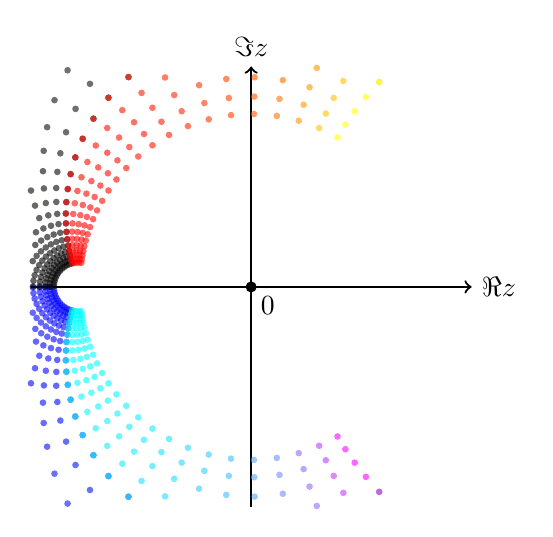
\begin{tikzpicture}[scale=0.8]

\draw[->, thick] (-3.5,0) -- (3.5,0) node[right] {$\Re z$};
\draw[->, thick] (0,-3.5) -- (0,3.5) node[above] {$\Im z$};

\fill (0,0) circle (2.5pt) node[below right] {$0$};

\fill[color={rgb,255:red,0; green,0; blue,255}, opacity=0.60] (-3.1961,-0.0052) circle (1.5pt);
\fill[color={rgb,255:red,0; green,0; blue,255}, opacity=0.60] (-3.2711,-0.0061) circle (1.5pt);
\fill[color={rgb,255:red,0; green,0; blue,255}, opacity=0.60] (-3.3592,-0.0072) circle (1.5pt);
\fill[color={rgb,255:red,0; green,0; blue,255}, opacity=0.60] (-3.4631,-0.0085) circle (1.5pt);
\fill[color={rgb,255:red,0; green,0; blue,255}, opacity=0.60] (-3.1285,-0.0515) circle (1.5pt);
\fill[color={rgb,255:red,0; green,0; blue,255}, opacity=0.60] (-3.1920,-0.0602) circle (1.5pt);
\fill[color={rgb,255:red,0; green,0; blue,255}, opacity=0.60] (-3.2662,-0.0705) circle (1.5pt);
\fill[color={rgb,255:red,0; green,0; blue,255}, opacity=0.60] (-3.3533,-0.0829) circle (1.5pt);
\fill[color={rgb,255:red,0; green,0; blue,255}, opacity=0.60] (-3.4559,-0.0980) circle (1.5pt);
\fill[color={rgb,255:red,0; green,0; blue,255}, opacity=0.60] (-3.1194,-0.0978) circle (1.5pt);
\fill[color={rgb,255:red,0; green,0; blue,255}, opacity=0.60] (-3.1811,-0.1141) circle (1.5pt);
\fill[color={rgb,255:red,0; green,0; blue,255}, opacity=0.60] (-3.2532,-0.1336) circle (1.5pt);
\fill[color={rgb,255:red,0; green,0; blue,255}, opacity=0.60] (-3.3376,-0.1570) circle (1.5pt);
\fill[color={rgb,255:red,0; green,0; blue,255}, opacity=0.60] (-3.4368,-0.1854) circle (1.5pt);
\fill[color={rgb,255:red,0; green,0; blue,255}, opacity=0.60] (-3.1048,-0.1424) circle (1.5pt);
\fill[color={rgb,255:red,0; green,0; blue,255}, opacity=0.60] (-3.1637,-0.1660) circle (1.5pt);
\fill[color={rgb,255:red,0; green,0; blue,255}, opacity=0.60] (-3.2324,-0.1942) circle (1.5pt);
\fill[color={rgb,255:red,0; green,0; blue,255}, opacity=0.60] (-3.3126,-0.2280) circle (1.5pt);
\fill[color={rgb,255:red,0; green,0; blue,255}, opacity=0.60] (-3.4064,-0.2688) circle (1.5pt);
\fill[color={rgb,255:red,0; green,0; blue,255}, opacity=0.60] (-3.0850,-0.1847) circle (1.5pt);
\fill[color={rgb,255:red,0; green,0; blue,255}, opacity=0.60] (-3.1402,-0.2151) circle (1.5pt);
\fill[color={rgb,255:red,0; green,0; blue,255}, opacity=0.60] (-3.2044,-0.2513) circle (1.5pt);
\fill[color={rgb,255:red,0; green,0; blue,255}, opacity=0.60] (-3.2789,-0.2946) circle (1.5pt);
\fill[color={rgb,255:red,0; green,0; blue,255}, opacity=0.60] (-3.3656,-0.3467) circle (1.5pt);
\fill[color={rgb,255:red,0; green,1; blue,254}, opacity=0.60] (-3.4669,-0.4099) circle (1.5pt);
\fill[color={rgb,255:red,0; green,0; blue,255}, opacity=0.60] (-3.0604,-0.2240) circle (1.5pt);
\fill[color={rgb,255:red,0; green,0; blue,255}, opacity=0.60] (-3.1112,-0.2606) circle (1.5pt);
\fill[color={rgb,255:red,0; green,0; blue,255}, opacity=0.60] (-3.1697,-0.3039) circle (1.5pt);
\fill[color={rgb,255:red,0; green,0; blue,255}, opacity=0.60] (-3.2374,-0.3556) circle (1.5pt);
\fill[color={rgb,255:red,0; green,0; blue,255}, opacity=0.60] (-3.3157,-0.4176) circle (1.5pt);
\fill[color={rgb,255:red,0; green,1; blue,254}, opacity=0.60] (-3.4062,-0.4923) circle (1.5pt);
\fill[color={rgb,255:red,0; green,0; blue,255}, opacity=0.60] (-3.0316,-0.2598) circle (1.5pt);
\fill[color={rgb,255:red,0; green,0; blue,255}, opacity=0.60] (-3.0771,-0.3017) circle (1.5pt);
\fill[color={rgb,255:red,0; green,0; blue,255}, opacity=0.60] (-3.1294,-0.3513) circle (1.5pt);
\fill[color={rgb,255:red,0; green,0; blue,255}, opacity=0.60] (-3.1893,-0.4102) circle (1.5pt);
\fill[color={rgb,255:red,0; green,0; blue,255}, opacity=0.60] (-3.2579,-0.4804) circle (1.5pt);
\fill[color={rgb,255:red,0; green,1; blue,254}, opacity=0.60] (-3.3365,-0.5646) circle (1.5pt);
\fill[color={rgb,255:red,0; green,1; blue,254}, opacity=0.60] (-3.4262,-0.6664) circle (1.5pt);
\fill[color={rgb,255:red,0; green,0; blue,255}, opacity=0.60] (-2.9991,-0.2916) circle (1.5pt);
\fill[color={rgb,255:red,0; green,0; blue,255}, opacity=0.60] (-3.0389,-0.3381) circle (1.5pt);
\fill[color={rgb,255:red,0; green,0; blue,255}, opacity=0.60] (-3.0842,-0.3929) circle (1.5pt);
\fill[color={rgb,255:red,0; green,0; blue,255}, opacity=0.60] (-3.1356,-0.4575) circle (1.5pt);
\fill[color={rgb,255:red,0; green,0; blue,255}, opacity=0.60] (-3.1939,-0.5343) circle (1.5pt);
\fill[color={rgb,255:red,0; green,1; blue,254}, opacity=0.60] (-3.2597,-0.6259) circle (1.5pt);
\fill[color={rgb,255:red,0; green,1; blue,254}, opacity=0.60] (-3.3335,-0.7357) circle (1.5pt);
\fill[color={rgb,255:red,0; green,2; blue,254}, opacity=0.60] (-3.4157,-0.8680) circle (1.5pt);
\fill[color={rgb,255:red,0; green,0; blue,255}, opacity=0.60] (-2.9635,-0.3191) circle (1.5pt);
\fill[color={rgb,255:red,0; green,0; blue,255}, opacity=0.60] (-2.9971,-0.3693) circle (1.5pt);
\fill[color={rgb,255:red,0; green,0; blue,255}, opacity=0.60] (-3.0350,-0.4281) circle (1.5pt);
\fill[color={rgb,255:red,0; green,0; blue,255}, opacity=0.60] (-3.0776,-0.4973) circle (1.5pt);
\fill[color={rgb,255:red,0; green,0; blue,255}, opacity=0.60] (-3.1251,-0.5790) circle (1.5pt);
\fill[color={rgb,255:red,0; green,1; blue,254}, opacity=0.60] (-3.1777,-0.6757) circle (1.5pt);
\fill[color={rgb,255:red,0; green,1; blue,254}, opacity=0.60] (-3.2355,-0.7907) circle (1.5pt);
\fill[color={rgb,255:red,0; green,2; blue,254}, opacity=0.60] (-3.2978,-0.9280) circle (1.5pt);
\fill[color={rgb,255:red,0; green,3; blue,253}, opacity=0.60] (-3.3636,-1.0926) circle (1.5pt);
\fill[color={rgb,255:red,0; green,4; blue,253}, opacity=0.60] (-3.4307,-1.2906) circle (1.5pt);
\fill[color={rgb,255:red,0; green,5; blue,252}, opacity=0.60] (-3.4950,-1.5295) circle (1.5pt);
\fill[color={rgb,255:red,0; green,0; blue,255}, opacity=0.60] (-2.9254,-0.3420) circle (1.5pt);
\fill[color={rgb,255:red,0; green,0; blue,255}, opacity=0.60] (-2.9527,-0.3950) circle (1.5pt);
\fill[color={rgb,255:red,0; green,0; blue,255}, opacity=0.60] (-2.9830,-0.4568) circle (1.5pt);
\fill[color={rgb,255:red,0; green,0; blue,255}, opacity=0.60] (-3.0164,-0.5292) circle (1.5pt);
\fill[color={rgb,255:red,0; green,0; blue,255}, opacity=0.60] (-3.0530,-0.6141) circle (1.5pt);
\fill[color={rgb,255:red,0; green,1; blue,254}, opacity=0.60] (-3.0925,-0.7139) circle (1.5pt);
\fill[color={rgb,255:red,0; green,1; blue,254}, opacity=0.60] (-3.1344,-0.8316) circle (1.5pt);
\fill[color={rgb,255:red,0; green,2; blue,254}, opacity=0.60] (-3.1776,-0.9708) circle (1.5pt);
\fill[color={rgb,255:red,0; green,3; blue,253}, opacity=0.60] (-3.2202,-1.1356) circle (1.5pt);
\fill[color={rgb,255:red,0; green,4; blue,253}, opacity=0.60] (-3.2592,-1.3312) circle (1.5pt);
\fill[color={rgb,255:red,0; green,5; blue,252}, opacity=0.60] (-3.2898,-1.5631) circle (1.5pt);
\fill[color={rgb,255:red,0; green,7; blue,251}, opacity=0.60] (-3.3048,-1.8375) circle (1.5pt);
\fill[color={rgb,255:red,0; green,10; blue,250}, opacity=0.60] (-3.2932,-2.1603) circle (1.5pt);
\fill[color={rgb,255:red,0; green,13; blue,248}, opacity=0.60] (-3.2393,-2.5360) circle (1.5pt);
\fill[color={rgb,255:red,0; green,17; blue,246}, opacity=0.60] (-3.1219,-2.9649) circle (1.5pt);
\fill[color={rgb,255:red,0; green,22; blue,244}, opacity=0.60] (-2.9142,-3.4392) circle (1.5pt);
\fill[color={rgb,255:red,0; green,0; blue,255}, opacity=0.60] (-2.8855,-0.3601) circle (1.5pt);
\fill[color={rgb,255:red,0; green,0; blue,255}, opacity=0.60] (-2.9062,-0.4151) circle (1.5pt);
\fill[color={rgb,255:red,0; green,0; blue,255}, opacity=0.60] (-2.9289,-0.4789) circle (1.5pt);
\fill[color={rgb,255:red,0; green,0; blue,255}, opacity=0.60] (-2.9532,-0.5532) circle (1.5pt);
\fill[color={rgb,255:red,0; green,0; blue,255}, opacity=0.60] (-2.9791,-0.6398) circle (1.5pt);
\fill[color={rgb,255:red,0; green,1; blue,254}, opacity=0.60] (-3.0058,-0.7408) circle (1.5pt);
\fill[color={rgb,255:red,0; green,1; blue,254}, opacity=0.60] (-3.0324,-0.8590) circle (1.5pt);
\fill[color={rgb,255:red,0; green,2; blue,254}, opacity=0.60] (-3.0576,-0.9974) circle (1.5pt);
\fill[color={rgb,255:red,0; green,3; blue,253}, opacity=0.60] (-3.0788,-1.1593) circle (1.5pt);
\fill[color={rgb,255:red,0; green,4; blue,253}, opacity=0.60] (-3.0928,-1.3487) circle (1.5pt);
\fill[color={rgb,255:red,0; green,5; blue,252}, opacity=0.60] (-3.0943,-1.5697) circle (1.5pt);
\fill[color={rgb,255:red,0; green,7; blue,251}, opacity=0.60] (-3.0763,-1.8262) circle (1.5pt);
\fill[color={rgb,255:red,0; green,10; blue,250}, opacity=0.60] (-3.0287,-2.1213) circle (1.5pt);
\fill[color={rgb,255:red,0; green,13; blue,248}, opacity=0.60] (-2.9381,-2.4559) circle (1.5pt);
\fill[color={rgb,255:red,0; green,17; blue,246}, opacity=0.60] (-2.7878,-2.8268) circle (1.5pt);
\fill[color={rgb,255:red,0; green,22; blue,244}, opacity=0.60] (-2.5585,-3.2238) circle (1.5pt);
\fill[color={rgb,255:red,0; green,0; blue,255}, opacity=0.60] (-2.8444,-0.3735) circle (1.5pt);
\fill[color={rgb,255:red,0; green,0; blue,255}, opacity=0.60] (-2.8586,-0.4295) circle (1.5pt);
\fill[color={rgb,255:red,0; green,0; blue,255}, opacity=0.60] (-2.8737,-0.4944) circle (1.5pt);
\fill[color={rgb,255:red,0; green,0; blue,255}, opacity=0.60] (-2.8891,-0.5694) circle (1.5pt);
\fill[color={rgb,255:red,0; green,0; blue,255}, opacity=0.60] (-2.9045,-0.6562) circle (1.5pt);
\fill[color={rgb,255:red,0; green,1; blue,254}, opacity=0.60] (-2.9190,-0.7570) circle (1.5pt);
\fill[color={rgb,255:red,0; green,1; blue,254}, opacity=0.60] (-2.9314,-0.8737) circle (1.5pt);
\fill[color={rgb,255:red,0; green,2; blue,254}, opacity=0.60] (-2.9399,-1.0090) circle (1.5pt);
\fill[color={rgb,255:red,0; green,3; blue,253}, opacity=0.60] (-2.9420,-1.1655) circle (1.5pt);
\fill[color={rgb,255:red,0; green,4; blue,253}, opacity=0.60] (-2.9340,-1.3461) circle (1.5pt);
\fill[color={rgb,255:red,0; green,5; blue,252}, opacity=0.60] (-2.9110,-1.5536) circle (1.5pt);
\fill[color={rgb,255:red,0; green,7; blue,251}, opacity=0.60] (-2.8663,-1.7902) circle (1.5pt);
\fill[color={rgb,255:red,0; green,10; blue,250}, opacity=0.60] (-2.7911,-2.0568) circle (1.5pt);
\fill[color={rgb,255:red,0; green,13; blue,248}, opacity=0.60] (-2.6746,-2.3521) circle (1.5pt);
\fill[color={rgb,255:red,0; green,17; blue,246}, opacity=0.60] (-2.5038,-2.6711) circle (1.5pt);
\fill[color={rgb,255:red,0; green,22; blue,244}, opacity=0.60] (-2.2654,-3.0033) circle (1.5pt);
\fill[color={rgb,255:red,0; green,29; blue,240}, opacity=0.60] (-1.9477,-3.3312) circle (1.5pt);
\fill[color={rgb,255:red,0; green,255; blue,127}, opacity=0.60] (2.0329,-3.2530) circle (1.5pt);
\fill[color={rgb,255:red,0; green,0; blue,0}, opacity=0.60] (-2.8444,0.3735) circle (1.5pt);
\fill[color={rgb,255:red,0; green,0; blue,0}, opacity=0.60] (-2.8586,0.4295) circle (1.5pt);
\fill[color={rgb,255:red,0; green,0; blue,0}, opacity=0.60] (-2.8737,0.4944) circle (1.5pt);
\fill[color={rgb,255:red,0; green,0; blue,0}, opacity=0.60] (-2.8891,0.5694) circle (1.5pt);
\fill[color={rgb,255:red,0; green,0; blue,0}, opacity=0.60] (-2.9045,0.6562) circle (1.5pt);
\fill[color={rgb,255:red,1; green,0; blue,0}, opacity=0.60] (-2.9190,0.7570) circle (1.5pt);
\fill[color={rgb,255:red,1; green,0; blue,0}, opacity=0.60] (-2.9314,0.8737) circle (1.5pt);
\fill[color={rgb,255:red,2; green,1; blue,0}, opacity=0.60] (-2.9399,1.0090) circle (1.5pt);
\fill[color={rgb,255:red,3; green,2; blue,1}, opacity=0.60] (-2.9420,1.1655) circle (1.5pt);
\fill[color={rgb,255:red,4; green,3; blue,1}, opacity=0.60] (-2.9340,1.3461) circle (1.5pt);
\fill[color={rgb,255:red,6; green,3; blue,2}, opacity=0.60] (-2.9110,1.5536) circle (1.5pt);
\fill[color={rgb,255:red,8; green,5; blue,3}, opacity=0.60] (-2.8663,1.7902) circle (1.5pt);
\fill[color={rgb,255:red,12; green,7; blue,4}, opacity=0.60] (-2.7911,2.0568) circle (1.5pt);
\fill[color={rgb,255:red,16; green,10; blue,6}, opacity=0.60] (-2.6746,2.3521) circle (1.5pt);
\fill[color={rgb,255:red,20; green,13; blue,8}, opacity=0.60] (-2.5038,2.6711) circle (1.5pt);
\fill[color={rgb,255:red,27; green,17; blue,10}, opacity=0.60] (-2.2654,3.0033) circle (1.5pt);
\fill[color={rgb,255:red,35; green,22; blue,14}, opacity=0.60] (-1.9477,3.3312) circle (1.5pt);
\fill[color={rgb,255:red,255; green,199; blue,126}, opacity=0.60] (2.0329,3.2530) circle (1.5pt);
\fill[color={rgb,255:red,0; green,0; blue,0}, opacity=0.60] (-2.8855,0.3601) circle (1.5pt);
\fill[color={rgb,255:red,0; green,0; blue,0}, opacity=0.60] (-2.9062,0.4151) circle (1.5pt);
\fill[color={rgb,255:red,0; green,0; blue,0}, opacity=0.60] (-2.9289,0.4789) circle (1.5pt);
\fill[color={rgb,255:red,0; green,0; blue,0}, opacity=0.60] (-2.9532,0.5532) circle (1.5pt);
\fill[color={rgb,255:red,0; green,0; blue,0}, opacity=0.60] (-2.9791,0.6398) circle (1.5pt);
\fill[color={rgb,255:red,1; green,0; blue,0}, opacity=0.60] (-3.0058,0.7408) circle (1.5pt);
\fill[color={rgb,255:red,1; green,0; blue,0}, opacity=0.60] (-3.0324,0.8590) circle (1.5pt);
\fill[color={rgb,255:red,2; green,1; blue,0}, opacity=0.60] (-3.0576,0.9974) circle (1.5pt);
\fill[color={rgb,255:red,3; green,2; blue,1}, opacity=0.60] (-3.0788,1.1593) circle (1.5pt);
\fill[color={rgb,255:red,4; green,3; blue,1}, opacity=0.60] (-3.0928,1.3487) circle (1.5pt);
\fill[color={rgb,255:red,6; green,3; blue,2}, opacity=0.60] (-3.0943,1.5697) circle (1.5pt);
\fill[color={rgb,255:red,8; green,5; blue,3}, opacity=0.60] (-3.0763,1.8262) circle (1.5pt);
\fill[color={rgb,255:red,12; green,7; blue,4}, opacity=0.60] (-3.0287,2.1213) circle (1.5pt);
\fill[color={rgb,255:red,16; green,10; blue,6}, opacity=0.60] (-2.9381,2.4559) circle (1.5pt);
\fill[color={rgb,255:red,20; green,13; blue,8}, opacity=0.60] (-2.7878,2.8268) circle (1.5pt);
\fill[color={rgb,255:red,27; green,17; blue,10}, opacity=0.60] (-2.5585,3.2238) circle (1.5pt);
\fill[color={rgb,255:red,0; green,0; blue,0}, opacity=0.60] (-2.9254,0.3420) circle (1.5pt);
\fill[color={rgb,255:red,0; green,0; blue,0}, opacity=0.60] (-2.9527,0.3950) circle (1.5pt);
\fill[color={rgb,255:red,0; green,0; blue,0}, opacity=0.60] (-2.9830,0.4568) circle (1.5pt);
\fill[color={rgb,255:red,0; green,0; blue,0}, opacity=0.60] (-3.0164,0.5292) circle (1.5pt);
\fill[color={rgb,255:red,0; green,0; blue,0}, opacity=0.60] (-3.0530,0.6141) circle (1.5pt);
\fill[color={rgb,255:red,1; green,0; blue,0}, opacity=0.60] (-3.0925,0.7139) circle (1.5pt);
\fill[color={rgb,255:red,1; green,0; blue,0}, opacity=0.60] (-3.1344,0.8316) circle (1.5pt);
\fill[color={rgb,255:red,2; green,1; blue,0}, opacity=0.60] (-3.1776,0.9708) circle (1.5pt);
\fill[color={rgb,255:red,3; green,2; blue,1}, opacity=0.60] (-3.2202,1.1356) circle (1.5pt);
\fill[color={rgb,255:red,4; green,3; blue,1}, opacity=0.60] (-3.2592,1.3312) circle (1.5pt);
\fill[color={rgb,255:red,6; green,3; blue,2}, opacity=0.60] (-3.2898,1.5631) circle (1.5pt);
\fill[color={rgb,255:red,8; green,5; blue,3}, opacity=0.60] (-3.3048,1.8375) circle (1.5pt);
\fill[color={rgb,255:red,12; green,7; blue,4}, opacity=0.60] (-3.2932,2.1603) circle (1.5pt);
\fill[color={rgb,255:red,16; green,10; blue,6}, opacity=0.60] (-3.2393,2.5360) circle (1.5pt);
\fill[color={rgb,255:red,20; green,13; blue,8}, opacity=0.60] (-3.1219,2.9649) circle (1.5pt);
\fill[color={rgb,255:red,27; green,17; blue,10}, opacity=0.60] (-2.9142,3.4392) circle (1.5pt);
\fill[color={rgb,255:red,0; green,0; blue,0}, opacity=0.60] (-2.9635,0.3191) circle (1.5pt);
\fill[color={rgb,255:red,0; green,0; blue,0}, opacity=0.60] (-2.9971,0.3693) circle (1.5pt);
\fill[color={rgb,255:red,0; green,0; blue,0}, opacity=0.60] (-3.0350,0.4281) circle (1.5pt);
\fill[color={rgb,255:red,0; green,0; blue,0}, opacity=0.60] (-3.0776,0.4973) circle (1.5pt);
\fill[color={rgb,255:red,0; green,0; blue,0}, opacity=0.60] (-3.1251,0.5790) circle (1.5pt);
\fill[color={rgb,255:red,1; green,0; blue,0}, opacity=0.60] (-3.1777,0.6757) circle (1.5pt);
\fill[color={rgb,255:red,1; green,0; blue,0}, opacity=0.60] (-3.2355,0.7907) circle (1.5pt);
\fill[color={rgb,255:red,2; green,1; blue,0}, opacity=0.60] (-3.2978,0.9280) circle (1.5pt);
\fill[color={rgb,255:red,3; green,2; blue,1}, opacity=0.60] (-3.3636,1.0926) circle (1.5pt);
\fill[color={rgb,255:red,4; green,3; blue,1}, opacity=0.60] (-3.4307,1.2906) circle (1.5pt);
\fill[color={rgb,255:red,6; green,3; blue,2}, opacity=0.60] (-3.4950,1.5295) circle (1.5pt);
\fill[color={rgb,255:red,0; green,0; blue,0}, opacity=0.60] (-2.9991,0.2916) circle (1.5pt);
\fill[color={rgb,255:red,0; green,0; blue,0}, opacity=0.60] (-3.0389,0.3381) circle (1.5pt);
\fill[color={rgb,255:red,0; green,0; blue,0}, opacity=0.60] (-3.0842,0.3929) circle (1.5pt);
\fill[color={rgb,255:red,0; green,0; blue,0}, opacity=0.60] (-3.1356,0.4575) circle (1.5pt);
\fill[color={rgb,255:red,0; green,0; blue,0}, opacity=0.60] (-3.1939,0.5343) circle (1.5pt);
\fill[color={rgb,255:red,1; green,0; blue,0}, opacity=0.60] (-3.2597,0.6259) circle (1.5pt);
\fill[color={rgb,255:red,1; green,0; blue,0}, opacity=0.60] (-3.3335,0.7357) circle (1.5pt);
\fill[color={rgb,255:red,2; green,1; blue,0}, opacity=0.60] (-3.4157,0.8680) circle (1.5pt);
\fill[color={rgb,255:red,0; green,0; blue,0}, opacity=0.60] (-3.0316,0.2598) circle (1.5pt);
\fill[color={rgb,255:red,0; green,0; blue,0}, opacity=0.60] (-3.0771,0.3017) circle (1.5pt);
\fill[color={rgb,255:red,0; green,0; blue,0}, opacity=0.60] (-3.1294,0.3513) circle (1.5pt);
\fill[color={rgb,255:red,0; green,0; blue,0}, opacity=0.60] (-3.1893,0.4102) circle (1.5pt);
\fill[color={rgb,255:red,0; green,0; blue,0}, opacity=0.60] (-3.2579,0.4804) circle (1.5pt);
\fill[color={rgb,255:red,1; green,0; blue,0}, opacity=0.60] (-3.3365,0.5646) circle (1.5pt);
\fill[color={rgb,255:red,1; green,0; blue,0}, opacity=0.60] (-3.4262,0.6664) circle (1.5pt);
\fill[color={rgb,255:red,0; green,0; blue,0}, opacity=0.60] (-3.0604,0.2240) circle (1.5pt);
\fill[color={rgb,255:red,0; green,0; blue,0}, opacity=0.60] (-3.1112,0.2606) circle (1.5pt);
\fill[color={rgb,255:red,0; green,0; blue,0}, opacity=0.60] (-3.1697,0.3039) circle (1.5pt);
\fill[color={rgb,255:red,0; green,0; blue,0}, opacity=0.60] (-3.2374,0.3556) circle (1.5pt);
\fill[color={rgb,255:red,0; green,0; blue,0}, opacity=0.60] (-3.3157,0.4176) circle (1.5pt);
\fill[color={rgb,255:red,1; green,0; blue,0}, opacity=0.60] (-3.4062,0.4923) circle (1.5pt);
\fill[color={rgb,255:red,0; green,0; blue,0}, opacity=0.60] (-3.0850,0.1847) circle (1.5pt);
\fill[color={rgb,255:red,0; green,0; blue,0}, opacity=0.60] (-3.1402,0.2151) circle (1.5pt);
\fill[color={rgb,255:red,0; green,0; blue,0}, opacity=0.60] (-3.2044,0.2513) circle (1.5pt);
\fill[color={rgb,255:red,0; green,0; blue,0}, opacity=0.60] (-3.2789,0.2946) circle (1.5pt);
\fill[color={rgb,255:red,0; green,0; blue,0}, opacity=0.60] (-3.3656,0.3467) circle (1.5pt);
\fill[color={rgb,255:red,1; green,0; blue,0}, opacity=0.60] (-3.4669,0.4099) circle (1.5pt);
\fill[color={rgb,255:red,0; green,0; blue,0}, opacity=0.60] (-3.1048,0.1424) circle (1.5pt);
\fill[color={rgb,255:red,0; green,0; blue,0}, opacity=0.60] (-3.1637,0.1660) circle (1.5pt);
\fill[color={rgb,255:red,0; green,0; blue,0}, opacity=0.60] (-3.2324,0.1942) circle (1.5pt);
\fill[color={rgb,255:red,0; green,0; blue,0}, opacity=0.60] (-3.3126,0.2280) circle (1.5pt);
\fill[color={rgb,255:red,0; green,0; blue,0}, opacity=0.60] (-3.4064,0.2688) circle (1.5pt);
\fill[color={rgb,255:red,0; green,0; blue,0}, opacity=0.60] (-3.1194,0.0978) circle (1.5pt);
\fill[color={rgb,255:red,0; green,0; blue,0}, opacity=0.60] (-3.1811,0.1141) circle (1.5pt);
\fill[color={rgb,255:red,0; green,0; blue,0}, opacity=0.60] (-3.2532,0.1336) circle (1.5pt);
\fill[color={rgb,255:red,0; green,0; blue,0}, opacity=0.60] (-3.3376,0.1570) circle (1.5pt);
\fill[color={rgb,255:red,0; green,0; blue,0}, opacity=0.60] (-3.4368,0.1854) circle (1.5pt);
\fill[color={rgb,255:red,0; green,0; blue,0}, opacity=0.60] (-3.1285,0.0515) circle (1.5pt);
\fill[color={rgb,255:red,0; green,0; blue,0}, opacity=0.60] (-3.1920,0.0602) circle (1.5pt);
\fill[color={rgb,255:red,0; green,0; blue,0}, opacity=0.60] (-3.2662,0.0705) circle (1.5pt);
\fill[color={rgb,255:red,0; green,0; blue,0}, opacity=0.60] (-3.3533,0.0829) circle (1.5pt);
\fill[color={rgb,255:red,0; green,0; blue,0}, opacity=0.60] (-3.4559,0.0980) circle (1.5pt);
\fill[color={rgb,255:red,0; green,0; blue,0}, opacity=0.60] (-3.1319,0.0045) circle (1.5pt);
\fill[color={rgb,255:red,0; green,0; blue,0}, opacity=0.60] (-3.1961,0.0052) circle (1.5pt);
\fill[color={rgb,255:red,0; green,0; blue,0}, opacity=0.60] (-3.2711,0.0061) circle (1.5pt);
\fill[color={rgb,255:red,0; green,0; blue,0}, opacity=0.60] (-3.3592,0.0072) circle (1.5pt);
\fill[color={rgb,255:red,0; green,0; blue,0}, opacity=0.60] (-3.4631,0.0085) circle (1.5pt);
\fill[color={rgb,255:red,0; green,255; blue,255}, opacity=0.60] (-2.8444,-0.3735) circle (1.5pt);
\fill[color={rgb,255:red,0; green,255; blue,255}, opacity=0.60] (-2.8586,-0.4295) circle (1.5pt);
\fill[color={rgb,255:red,0; green,255; blue,255}, opacity=0.60] (-2.8737,-0.4944) circle (1.5pt);
\fill[color={rgb,255:red,0; green,255; blue,255}, opacity=0.60] (-2.8891,-0.5694) circle (1.5pt);
\fill[color={rgb,255:red,0; green,255; blue,255}, opacity=0.60] (-2.9045,-0.6562) circle (1.5pt);
\fill[color={rgb,255:red,1; green,254; blue,255}, opacity=0.60] (-2.9190,-0.7570) circle (1.5pt);
\fill[color={rgb,255:red,1; green,254; blue,255}, opacity=0.60] (-2.9314,-0.8737) circle (1.5pt);
\fill[color={rgb,255:red,2; green,253; blue,255}, opacity=0.60] (-2.9399,-1.0090) circle (1.5pt);
\fill[color={rgb,255:red,3; green,252; blue,255}, opacity=0.60] (-2.9420,-1.1655) circle (1.5pt);
\fill[color={rgb,255:red,4; green,251; blue,255}, opacity=0.60] (-2.9340,-1.3461) circle (1.5pt);
\fill[color={rgb,255:red,5; green,250; blue,255}, opacity=0.60] (-2.9110,-1.5536) circle (1.5pt);
\fill[color={rgb,255:red,7; green,248; blue,255}, opacity=0.60] (-2.8663,-1.7902) circle (1.5pt);
\fill[color={rgb,255:red,10; green,245; blue,255}, opacity=0.60] (-2.7911,-2.0568) circle (1.5pt);
\fill[color={rgb,255:red,13; green,242; blue,255}, opacity=0.60] (-2.6746,-2.3521) circle (1.5pt);
\fill[color={rgb,255:red,17; green,238; blue,255}, opacity=0.60] (-2.5038,-2.6711) circle (1.5pt);
\fill[color={rgb,255:red,22; green,233; blue,255}, opacity=0.60] (-2.2654,-3.0033) circle (1.5pt);
\fill[color={rgb,255:red,29; green,226; blue,255}, opacity=0.60] (-1.9477,-3.3312) circle (1.5pt);
\fill[color={rgb,255:red,255; green,0; blue,255}, opacity=0.60] (2.0329,-3.2530) circle (1.5pt);
\fill[color={rgb,255:red,0; green,255; blue,255}, opacity=0.60] (-2.8068,-0.3815) circle (1.5pt);
\fill[color={rgb,255:red,0; green,255; blue,255}, opacity=0.60] (-2.8153,-0.4378) circle (1.5pt);
\fill[color={rgb,255:red,0; green,255; blue,255}, opacity=0.60] (-2.8236,-0.5027) circle (1.5pt);
\fill[color={rgb,255:red,0; green,255; blue,255}, opacity=0.60] (-2.8313,-0.5775) circle (1.5pt);
\fill[color={rgb,255:red,0; green,255; blue,255}, opacity=0.60] (-2.8378,-0.6636) circle (1.5pt);
\fill[color={rgb,255:red,1; green,254; blue,255}, opacity=0.60] (-2.8419,-0.7628) circle (1.5pt);
\fill[color={rgb,255:red,1; green,254; blue,255}, opacity=0.60] (-2.8424,-0.8768) circle (1.5pt);
\fill[color={rgb,255:red,2; green,253; blue,255}, opacity=0.60] (-2.8373,-1.0078) circle (1.5pt);
\fill[color={rgb,255:red,3; green,252; blue,255}, opacity=0.60] (-2.8240,-1.1579) circle (1.5pt);
\fill[color={rgb,255:red,4; green,251; blue,255}, opacity=0.60] (-2.7990,-1.3291) circle (1.5pt);
\fill[color={rgb,255:red,5; green,250; blue,255}, opacity=0.60] (-2.7575,-1.5232) circle (1.5pt);
\fill[color={rgb,255:red,7; green,248; blue,255}, opacity=0.60] (-2.6935,-1.7411) circle (1.5pt);
\fill[color={rgb,255:red,10; green,245; blue,255}, opacity=0.60] (-2.5995,-1.9826) circle (1.5pt);
\fill[color={rgb,255:red,13; green,242; blue,255}, opacity=0.60] (-2.4666,-2.2452) circle (1.5pt);
\fill[color={rgb,255:red,17; green,238; blue,255}, opacity=0.60] (-2.2851,-2.5231) circle (1.5pt);
\fill[color={rgb,255:red,22; green,233; blue,255}, opacity=0.60] (-2.0453,-2.8064) circle (1.5pt);
\fill[color={rgb,255:red,29; green,226; blue,255}, opacity=0.60] (-1.7400,-3.0801) circle (1.5pt);
\fill[color={rgb,255:red,39; green,216; blue,255}, opacity=0.60] (-1.3666,-3.3247) circle (1.5pt);
\fill[color={rgb,255:red,150; green,105; blue,255}, opacity=0.60] (1.0419,-3.4769) circle (1.5pt);
\fill[color={rgb,255:red,195; green,59; blue,255}, opacity=0.60] (1.4637,-3.2690) circle (1.5pt);
\fill[color={rgb,255:red,255; green,0; blue,255}, opacity=0.60] (1.8206,-3.0153) circle (1.5pt);
\fill[color={rgb,255:red,0; green,255; blue,255}, opacity=0.60] (-2.7692,-0.3856) circle (1.5pt);
\fill[color={rgb,255:red,0; green,255; blue,255}, opacity=0.60] (-2.7720,-0.4417) circle (1.5pt);
\fill[color={rgb,255:red,0; green,255; blue,255}, opacity=0.60] (-2.7739,-0.5061) circle (1.5pt);
\fill[color={rgb,255:red,0; green,255; blue,255}, opacity=0.60] (-2.7742,-0.5798) circle (1.5pt);
\fill[color={rgb,255:red,0; green,255; blue,255}, opacity=0.60] (-2.7722,-0.6643) circle (1.5pt);
\fill[color={rgb,255:red,1; green,254; blue,255}, opacity=0.60] (-2.7667,-0.7609) circle (1.5pt);
\fill[color={rgb,255:red,1; green,254; blue,255}, opacity=0.60] (-2.7562,-0.8712) circle (1.5pt);
\fill[color={rgb,255:red,2; green,253; blue,255}, opacity=0.60] (-2.7389,-0.9969) circle (1.5pt);
\fill[color={rgb,255:red,3; green,252; blue,255}, opacity=0.60] (-2.7120,-1.1394) circle (1.5pt);
\fill[color={rgb,255:red,4; green,251; blue,255}, opacity=0.60] (-2.6723,-1.3003) circle (1.5pt);
\fill[color={rgb,255:red,5; green,250; blue,255}, opacity=0.60] (-2.6154,-1.4803) circle (1.5pt);
\fill[color={rgb,255:red,7; green,248; blue,255}, opacity=0.60] (-2.5360,-1.6798) circle (1.5pt);
\fill[color={rgb,255:red,10; green,245; blue,255}, opacity=0.60] (-2.4279,-1.8974) circle (1.5pt);
\fill[color={rgb,255:red,13; green,242; blue,255}, opacity=0.60] (-2.2838,-2.1300) circle (1.5pt);
\fill[color={rgb,255:red,17; green,238; blue,255}, opacity=0.60] (-2.0965,-2.3719) circle (1.5pt);
\fill[color={rgb,255:red,22; green,233; blue,255}, opacity=0.60] (-1.8592,-2.6140) circle (1.5pt);
\fill[color={rgb,255:red,29; green,226; blue,255}, opacity=0.60] (-1.5678,-2.8437) circle (1.5pt);
\fill[color={rgb,255:red,39; green,216; blue,255}, opacity=0.60] (-1.2218,-3.0457) circle (1.5pt);
\fill[color={rgb,255:red,51; green,204; blue,255}, opacity=0.60] (-0.8269,-3.2031) circle (1.5pt);
\fill[color={rgb,255:red,67; green,188; blue,255}, opacity=0.60] (-0.3952,-3.3009) circle (1.5pt);
\fill[color={rgb,255:red,87; green,168; blue,255}, opacity=0.60] (0.0551,-3.3286) circle (1.5pt);
\fill[color={rgb,255:red,113; green,141; blue,255}, opacity=0.60] (0.5028,-3.2832) circle (1.5pt);
\fill[color={rgb,255:red,150; green,105; blue,255}, opacity=0.60] (0.9270,-3.1697) circle (1.5pt);
\fill[color={rgb,255:red,195; green,59; blue,255}, opacity=0.60] (1.3109,-2.9999) circle (1.5pt);
\fill[color={rgb,255:red,255; green,0; blue,255}, opacity=0.60] (1.6439,-2.7897) circle (1.5pt);
\fill[color={rgb,255:red,0; green,255; blue,255}, opacity=0.60] (-2.7318,-0.3861) circle (1.5pt);
\fill[color={rgb,255:red,0; green,255; blue,255}, opacity=0.60] (-2.7292,-0.4414) circle (1.5pt);
\fill[color={rgb,255:red,0; green,255; blue,255}, opacity=0.60] (-2.7250,-0.5046) circle (1.5pt);
\fill[color={rgb,255:red,0; green,255; blue,255}, opacity=0.60] (-2.7183,-0.5766) circle (1.5pt);
\fill[color={rgb,255:red,0; green,255; blue,255}, opacity=0.60] (-2.7083,-0.6586) circle (1.5pt);
\fill[color={rgb,255:red,1; green,254; blue,255}, opacity=0.60] (-2.6939,-0.7519) circle (1.5pt);
\fill[color={rgb,255:red,1; green,254; blue,255}, opacity=0.60] (-2.6736,-0.8577) circle (1.5pt);
\fill[color={rgb,255:red,2; green,253; blue,255}, opacity=0.60] (-2.6453,-0.9772) circle (1.5pt);
\fill[color={rgb,255:red,3; green,252; blue,255}, opacity=0.60] (-2.6066,-1.1115) circle (1.5pt);
\fill[color={rgb,255:red,4; green,251; blue,255}, opacity=0.60] (-2.5544,-1.2615) circle (1.5pt);
\fill[color={rgb,255:red,5; green,250; blue,255}, opacity=0.60] (-2.4849,-1.4275) circle (1.5pt);
\fill[color={rgb,255:red,7; green,248; blue,255}, opacity=0.60] (-2.3934,-1.6089) circle (1.5pt);
\fill[color={rgb,255:red,10; green,245; blue,255}, opacity=0.60] (-2.2747,-1.8042) circle (1.5pt);
\fill[color={rgb,255:red,13; green,242; blue,255}, opacity=0.60] (-2.1233,-2.0099) circle (1.5pt);
\fill[color={rgb,255:red,17; green,238; blue,255}, opacity=0.60] (-1.9337,-2.2204) circle (1.5pt);
\fill[color={rgb,255:red,22; green,233; blue,255}, opacity=0.60] (-1.7014,-2.4278) circle (1.5pt);
\fill[color={rgb,255:red,29; green,226; blue,255}, opacity=0.60] (-1.4241,-2.6216) circle (1.5pt);
\fill[color={rgb,255:red,39; green,216; blue,255}, opacity=0.60] (-1.1026,-2.7896) circle (1.5pt);
\fill[color={rgb,255:red,51; green,204; blue,255}, opacity=0.60] (-0.7425,-2.9191) circle (1.5pt);
\fill[color={rgb,255:red,67; green,188; blue,255}, opacity=0.60] (-0.3538,-2.9989) circle (1.5pt);
\fill[color={rgb,255:red,87; green,168; blue,255}, opacity=0.60] (0.0493,-3.0214) circle (1.5pt);
\fill[color={rgb,255:red,113; green,141; blue,255}, opacity=0.60] (0.4504,-2.9845) circle (1.5pt);
\fill[color={rgb,255:red,150; green,105; blue,255}, opacity=0.60] (0.8333,-2.8918) circle (1.5pt);
\fill[color={rgb,255:red,195; green,59; blue,255}, opacity=0.60] (1.1848,-2.7518) circle (1.5pt);
\fill[color={rgb,255:red,255; green,0; blue,255}, opacity=0.60] (1.4958,-2.5763) circle (1.5pt);
\fill[color={rgb,255:red,0; green,255; blue,255}, opacity=0.60] (-2.6950,-0.3830) circle (1.5pt);
\fill[color={rgb,255:red,0; green,255; blue,255}, opacity=0.60] (-2.6873,-0.4371) circle (1.5pt);
\fill[color={rgb,255:red,0; green,255; blue,255}, opacity=0.60] (-2.6772,-0.4985) circle (1.5pt);
\fill[color={rgb,255:red,0; green,255; blue,255}, opacity=0.60] (-2.6640,-0.5682) circle (1.5pt);
\fill[color={rgb,255:red,0; green,255; blue,255}, opacity=0.60] (-2.6468,-0.6472) circle (1.5pt);
\fill[color={rgb,255:red,1; green,254; blue,255}, opacity=0.60] (-2.6242,-0.7365) circle (1.5pt);
\fill[color={rgb,255:red,1; green,254; blue,255}, opacity=0.60] (-2.5950,-0.8371) circle (1.5pt);
\fill[color={rgb,255:red,2; green,253; blue,255}, opacity=0.60] (-2.5571,-0.9498) circle (1.5pt);
\fill[color={rgb,255:red,3; green,252; blue,255}, opacity=0.60] (-2.5082,-1.0754) circle (1.5pt);
\fill[color={rgb,255:red,4; green,251; blue,255}, opacity=0.60] (-2.4455,-1.2144) circle (1.5pt);
\fill[color={rgb,255:red,5; green,250; blue,255}, opacity=0.60] (-2.3656,-1.3665) circle (1.5pt);
\fill[color={rgb,255:red,7; green,248; blue,255}, opacity=0.60] (-2.2647,-1.5309) circle (1.5pt);
\fill[color={rgb,255:red,10; green,245; blue,255}, opacity=0.60] (-2.1384,-1.7056) circle (1.5pt);
\fill[color={rgb,255:red,13; green,242; blue,255}, opacity=0.60] (-1.9826,-1.8871) circle (1.5pt);
\fill[color={rgb,255:red,17; green,238; blue,255}, opacity=0.60] (-1.7931,-2.0704) circle (1.5pt);
\fill[color={rgb,255:red,22; green,233; blue,255}, opacity=0.60] (-1.5670,-2.2485) circle (1.5pt);
\fill[color={rgb,255:red,29; green,226; blue,255}, opacity=0.60] (-1.3034,-2.4128) circle (1.5pt);
\fill[color={rgb,255:red,39; green,216; blue,255}, opacity=0.60] (-1.0037,-2.5535) circle (1.5pt);
\fill[color={rgb,255:red,51; green,204; blue,255}, opacity=0.60] (-0.6731,-2.6610) circle (1.5pt);
\fill[color={rgb,255:red,67; green,188; blue,255}, opacity=0.60] (-0.3199,-2.7267) circle (1.5pt);
\fill[color={rgb,255:red,87; green,168; blue,255}, opacity=0.60] (0.0446,-2.7452) circle (1.5pt);
\fill[color={rgb,255:red,113; green,141; blue,255}, opacity=0.60] (0.4074,-2.7149) circle (1.5pt);
\fill[color={rgb,255:red,150; green,105; blue,255}, opacity=0.60] (0.7561,-2.6383) circle (1.5pt);
\fill[color={rgb,255:red,195; green,59; blue,255}, opacity=0.60] (1.0798,-2.5219) circle (1.5pt);
\fill[color={rgb,255:red,255; green,0; blue,255}, opacity=0.60] (1.3710,-2.3745) circle (1.5pt);
\fill[color={rgb,255:red,255; green,0; blue,0}, opacity=0.60] (-2.6950,0.3830) circle (1.5pt);
\fill[color={rgb,255:red,255; green,0; blue,0}, opacity=0.60] (-2.6873,0.4371) circle (1.5pt);
\fill[color={rgb,255:red,255; green,0; blue,0}, opacity=0.60] (-2.6772,0.4985) circle (1.5pt);
\fill[color={rgb,255:red,255; green,0; blue,0}, opacity=0.60] (-2.6640,0.5682) circle (1.5pt);
\fill[color={rgb,255:red,255; green,0; blue,0}, opacity=0.60] (-2.6468,0.6472) circle (1.5pt);
\fill[color={rgb,255:red,255; green,1; blue,0}, opacity=0.60] (-2.6242,0.7365) circle (1.5pt);
\fill[color={rgb,255:red,255; green,1; blue,0}, opacity=0.60] (-2.5950,0.8371) circle (1.5pt);
\fill[color={rgb,255:red,255; green,2; blue,0}, opacity=0.60] (-2.5571,0.9498) circle (1.5pt);
\fill[color={rgb,255:red,255; green,3; blue,0}, opacity=0.60] (-2.5082,1.0754) circle (1.5pt);
\fill[color={rgb,255:red,255; green,4; blue,0}, opacity=0.60] (-2.4455,1.2144) circle (1.5pt);
\fill[color={rgb,255:red,255; green,5; blue,0}, opacity=0.60] (-2.3656,1.3665) circle (1.5pt);
\fill[color={rgb,255:red,255; green,7; blue,0}, opacity=0.60] (-2.2647,1.5309) circle (1.5pt);
\fill[color={rgb,255:red,255; green,10; blue,0}, opacity=0.60] (-2.1384,1.7056) circle (1.5pt);
\fill[color={rgb,255:red,255; green,13; blue,0}, opacity=0.60] (-1.9826,1.8871) circle (1.5pt);
\fill[color={rgb,255:red,255; green,17; blue,0}, opacity=0.60] (-1.7931,2.0704) circle (1.5pt);
\fill[color={rgb,255:red,255; green,22; blue,0}, opacity=0.60] (-1.5670,2.2485) circle (1.5pt);
\fill[color={rgb,255:red,255; green,29; blue,0}, opacity=0.60] (-1.3034,2.4128) circle (1.5pt);
\fill[color={rgb,255:red,255; green,39; blue,0}, opacity=0.60] (-1.0037,2.5535) circle (1.5pt);
\fill[color={rgb,255:red,255; green,51; blue,0}, opacity=0.60] (-0.6731,2.6610) circle (1.5pt);
\fill[color={rgb,255:red,255; green,67; blue,0}, opacity=0.60] (-0.3199,2.7267) circle (1.5pt);
\fill[color={rgb,255:red,255; green,87; blue,0}, opacity=0.60] (0.0446,2.7452) circle (1.5pt);
\fill[color={rgb,255:red,255; green,113; blue,0}, opacity=0.60] (0.4074,2.7149) circle (1.5pt);
\fill[color={rgb,255:red,255; green,150; blue,0}, opacity=0.60] (0.7561,2.6383) circle (1.5pt);
\fill[color={rgb,255:red,255; green,195; blue,0}, opacity=0.60] (1.0798,2.5219) circle (1.5pt);
\fill[color={rgb,255:red,255; green,255; blue,0}, opacity=0.60] (1.3710,2.3745) circle (1.5pt);
\fill[color={rgb,255:red,255; green,0; blue,0}, opacity=0.60] (-2.7318,0.3861) circle (1.5pt);
\fill[color={rgb,255:red,255; green,0; blue,0}, opacity=0.60] (-2.7292,0.4414) circle (1.5pt);
\fill[color={rgb,255:red,255; green,0; blue,0}, opacity=0.60] (-2.7250,0.5046) circle (1.5pt);
\fill[color={rgb,255:red,255; green,0; blue,0}, opacity=0.60] (-2.7183,0.5766) circle (1.5pt);
\fill[color={rgb,255:red,255; green,0; blue,0}, opacity=0.60] (-2.7083,0.6586) circle (1.5pt);
\fill[color={rgb,255:red,255; green,1; blue,0}, opacity=0.60] (-2.6939,0.7519) circle (1.5pt);
\fill[color={rgb,255:red,255; green,1; blue,0}, opacity=0.60] (-2.6736,0.8577) circle (1.5pt);
\fill[color={rgb,255:red,255; green,2; blue,0}, opacity=0.60] (-2.6453,0.9772) circle (1.5pt);
\fill[color={rgb,255:red,255; green,3; blue,0}, opacity=0.60] (-2.6066,1.1115) circle (1.5pt);
\fill[color={rgb,255:red,255; green,4; blue,0}, opacity=0.60] (-2.5544,1.2615) circle (1.5pt);
\fill[color={rgb,255:red,255; green,5; blue,0}, opacity=0.60] (-2.4849,1.4275) circle (1.5pt);
\fill[color={rgb,255:red,255; green,7; blue,0}, opacity=0.60] (-2.3934,1.6089) circle (1.5pt);
\fill[color={rgb,255:red,255; green,10; blue,0}, opacity=0.60] (-2.2747,1.8042) circle (1.5pt);
\fill[color={rgb,255:red,255; green,13; blue,0}, opacity=0.60] (-2.1233,2.0099) circle (1.5pt);
\fill[color={rgb,255:red,255; green,17; blue,0}, opacity=0.60] (-1.9337,2.2204) circle (1.5pt);
\fill[color={rgb,255:red,255; green,22; blue,0}, opacity=0.60] (-1.7014,2.4278) circle (1.5pt);
\fill[color={rgb,255:red,255; green,29; blue,0}, opacity=0.60] (-1.4241,2.6216) circle (1.5pt);
\fill[color={rgb,255:red,255; green,39; blue,0}, opacity=0.60] (-1.1026,2.7896) circle (1.5pt);
\fill[color={rgb,255:red,255; green,51; blue,0}, opacity=0.60] (-0.7425,2.9191) circle (1.5pt);
\fill[color={rgb,255:red,255; green,67; blue,0}, opacity=0.60] (-0.3538,2.9989) circle (1.5pt);
\fill[color={rgb,255:red,255; green,87; blue,0}, opacity=0.60] (0.0493,3.0214) circle (1.5pt);
\fill[color={rgb,255:red,255; green,113; blue,0}, opacity=0.60] (0.4504,2.9845) circle (1.5pt);
\fill[color={rgb,255:red,255; green,150; blue,0}, opacity=0.60] (0.8333,2.8918) circle (1.5pt);
\fill[color={rgb,255:red,255; green,195; blue,0}, opacity=0.60] (1.1848,2.7518) circle (1.5pt);
\fill[color={rgb,255:red,255; green,255; blue,0}, opacity=0.60] (1.4958,2.5763) circle (1.5pt);
\fill[color={rgb,255:red,255; green,0; blue,0}, opacity=0.60] (-2.7692,0.3856) circle (1.5pt);
\fill[color={rgb,255:red,255; green,0; blue,0}, opacity=0.60] (-2.7720,0.4417) circle (1.5pt);
\fill[color={rgb,255:red,255; green,0; blue,0}, opacity=0.60] (-2.7739,0.5061) circle (1.5pt);
\fill[color={rgb,255:red,255; green,0; blue,0}, opacity=0.60] (-2.7742,0.5798) circle (1.5pt);
\fill[color={rgb,255:red,255; green,0; blue,0}, opacity=0.60] (-2.7722,0.6643) circle (1.5pt);
\fill[color={rgb,255:red,255; green,1; blue,0}, opacity=0.60] (-2.7667,0.7609) circle (1.5pt);
\fill[color={rgb,255:red,255; green,1; blue,0}, opacity=0.60] (-2.7562,0.8712) circle (1.5pt);
\fill[color={rgb,255:red,255; green,2; blue,0}, opacity=0.60] (-2.7389,0.9969) circle (1.5pt);
\fill[color={rgb,255:red,255; green,3; blue,0}, opacity=0.60] (-2.7120,1.1394) circle (1.5pt);
\fill[color={rgb,255:red,255; green,4; blue,0}, opacity=0.60] (-2.6723,1.3003) circle (1.5pt);
\fill[color={rgb,255:red,255; green,5; blue,0}, opacity=0.60] (-2.6154,1.4803) circle (1.5pt);
\fill[color={rgb,255:red,255; green,7; blue,0}, opacity=0.60] (-2.5360,1.6798) circle (1.5pt);
\fill[color={rgb,255:red,255; green,10; blue,0}, opacity=0.60] (-2.4279,1.8974) circle (1.5pt);
\fill[color={rgb,255:red,255; green,13; blue,0}, opacity=0.60] (-2.2838,2.1300) circle (1.5pt);
\fill[color={rgb,255:red,255; green,17; blue,0}, opacity=0.60] (-2.0965,2.3719) circle (1.5pt);
\fill[color={rgb,255:red,255; green,22; blue,0}, opacity=0.60] (-1.8592,2.6140) circle (1.5pt);
\fill[color={rgb,255:red,255; green,29; blue,0}, opacity=0.60] (-1.5678,2.8437) circle (1.5pt);
\fill[color={rgb,255:red,255; green,39; blue,0}, opacity=0.60] (-1.2218,3.0457) circle (1.5pt);
\fill[color={rgb,255:red,255; green,51; blue,0}, opacity=0.60] (-0.8269,3.2031) circle (1.5pt);
\fill[color={rgb,255:red,255; green,67; blue,0}, opacity=0.60] (-0.3952,3.3009) circle (1.5pt);
\fill[color={rgb,255:red,255; green,87; blue,0}, opacity=0.60] (0.0551,3.3286) circle (1.5pt);
\fill[color={rgb,255:red,255; green,113; blue,0}, opacity=0.60] (0.5028,3.2832) circle (1.5pt);
\fill[color={rgb,255:red,255; green,150; blue,0}, opacity=0.60] (0.9270,3.1697) circle (1.5pt);
\fill[color={rgb,255:red,255; green,195; blue,0}, opacity=0.60] (1.3109,2.9999) circle (1.5pt);
\fill[color={rgb,255:red,255; green,255; blue,0}, opacity=0.60] (1.6439,2.7897) circle (1.5pt);
\fill[color={rgb,255:red,255; green,0; blue,0}, opacity=0.60] (-2.8068,0.3815) circle (1.5pt);
\fill[color={rgb,255:red,255; green,0; blue,0}, opacity=0.60] (-2.8153,0.4378) circle (1.5pt);
\fill[color={rgb,255:red,255; green,0; blue,0}, opacity=0.60] (-2.8236,0.5027) circle (1.5pt);
\fill[color={rgb,255:red,255; green,0; blue,0}, opacity=0.60] (-2.8313,0.5775) circle (1.5pt);
\fill[color={rgb,255:red,255; green,0; blue,0}, opacity=0.60] (-2.8378,0.6636) circle (1.5pt);
\fill[color={rgb,255:red,255; green,1; blue,0}, opacity=0.60] (-2.8419,0.7628) circle (1.5pt);
\fill[color={rgb,255:red,255; green,1; blue,0}, opacity=0.60] (-2.8424,0.8768) circle (1.5pt);
\fill[color={rgb,255:red,255; green,2; blue,0}, opacity=0.60] (-2.8373,1.0078) circle (1.5pt);
\fill[color={rgb,255:red,255; green,3; blue,0}, opacity=0.60] (-2.8240,1.1579) circle (1.5pt);
\fill[color={rgb,255:red,255; green,4; blue,0}, opacity=0.60] (-2.7990,1.3291) circle (1.5pt);
\fill[color={rgb,255:red,255; green,5; blue,0}, opacity=0.60] (-2.7575,1.5232) circle (1.5pt);
\fill[color={rgb,255:red,255; green,7; blue,0}, opacity=0.60] (-2.6935,1.7411) circle (1.5pt);
\fill[color={rgb,255:red,255; green,10; blue,0}, opacity=0.60] (-2.5995,1.9826) circle (1.5pt);
\fill[color={rgb,255:red,255; green,13; blue,0}, opacity=0.60] (-2.4666,2.2452) circle (1.5pt);
\fill[color={rgb,255:red,255; green,17; blue,0}, opacity=0.60] (-2.2851,2.5231) circle (1.5pt);
\fill[color={rgb,255:red,255; green,22; blue,0}, opacity=0.60] (-2.0453,2.8064) circle (1.5pt);
\fill[color={rgb,255:red,255; green,29; blue,0}, opacity=0.60] (-1.7400,3.0801) circle (1.5pt);
\fill[color={rgb,255:red,255; green,39; blue,0}, opacity=0.60] (-1.3666,3.3247) circle (1.5pt);
\fill[color={rgb,255:red,255; green,150; blue,0}, opacity=0.60] (1.0419,3.4769) circle (1.5pt);
\fill[color={rgb,255:red,255; green,195; blue,0}, opacity=0.60] (1.4637,3.2690) circle (1.5pt);
\fill[color={rgb,255:red,255; green,255; blue,0}, opacity=0.60] (1.8206,3.0153) circle (1.5pt);
\fill[color={rgb,255:red,255; green,0; blue,0}, opacity=0.60] (-2.8444,0.3735) circle (1.5pt);
\fill[color={rgb,255:red,255; green,0; blue,0}, opacity=0.60] (-2.8586,0.4295) circle (1.5pt);
\fill[color={rgb,255:red,255; green,0; blue,0}, opacity=0.60] (-2.8737,0.4944) circle (1.5pt);
\fill[color={rgb,255:red,255; green,0; blue,0}, opacity=0.60] (-2.8891,0.5694) circle (1.5pt);
\fill[color={rgb,255:red,255; green,0; blue,0}, opacity=0.60] (-2.9045,0.6562) circle (1.5pt);
\fill[color={rgb,255:red,255; green,1; blue,0}, opacity=0.60] (-2.9190,0.7570) circle (1.5pt);
\fill[color={rgb,255:red,255; green,1; blue,0}, opacity=0.60] (-2.9314,0.8737) circle (1.5pt);
\fill[color={rgb,255:red,255; green,2; blue,0}, opacity=0.60] (-2.9399,1.0090) circle (1.5pt);
\fill[color={rgb,255:red,255; green,3; blue,0}, opacity=0.60] (-2.9420,1.1655) circle (1.5pt);
\fill[color={rgb,255:red,255; green,4; blue,0}, opacity=0.60] (-2.9340,1.3461) circle (1.5pt);
\fill[color={rgb,255:red,255; green,5; blue,0}, opacity=0.60] (-2.9110,1.5536) circle (1.5pt);
\fill[color={rgb,255:red,255; green,7; blue,0}, opacity=0.60] (-2.8663,1.7902) circle (1.5pt);
\fill[color={rgb,255:red,255; green,10; blue,0}, opacity=0.60] (-2.7911,2.0568) circle (1.5pt);
\fill[color={rgb,255:red,255; green,13; blue,0}, opacity=0.60] (-2.6746,2.3521) circle (1.5pt);
\fill[color={rgb,255:red,255; green,17; blue,0}, opacity=0.60] (-2.5038,2.6711) circle (1.5pt);
\fill[color={rgb,255:red,255; green,22; blue,0}, opacity=0.60] (-2.2654,3.0033) circle (1.5pt);
\fill[color={rgb,255:red,255; green,29; blue,0}, opacity=0.60] (-1.9477,3.3312) circle (1.5pt);
\fill[color={rgb,255:red,255; green,255; blue,0}, opacity=0.60] (2.0329,3.2530) circle (1.5pt);

\end{tikzpicture}\\
    Множество \( P_4=\omega_4(P_3) \) & Множество \( P_5=\omega_5(P_4)=Q \) \\
  \end{tabular}
\end{center}